\chapter{Sensitivitätsanalyse}\label{ch:Sensitivity}
In diesem Kapitel wird das in Kapitel \ref{ch:ch2} hergeleitete nichtlineare Modell des Antriebsstrangs auf die Sensitivität verschiedener Parameter und Eingänge untersucht. Damit soll die Relevanz für eine Parameter- und Eingangsschätzung im folgenden Kapitel belegt und unterstrichen werden.
Eine mögliche Definition für eine Sensitivitätsanalyse ist die folgende: \emph{The study of how uncertainty in the output of a model (numerical or otherwise) can be apportioned to different sources of uncertainty in the model input} \cite{Saltelli.2004}.
Für die Analyse gibt es verschiedene Methoden. Dabei ist die OAT(one-at-a-time)-Methode wohl die einfachste. Hier wird pro Simulationsdurchlauf lediglich eine Eingangsgröße geändert während alle anderen auf den nominal Werten gehalten werden. Die Methode liefert aber nur eine sehr beschränkte Aussage über den gesamten Eingangsraum. Jedoch kann sie für die Abschätzung einer ersten Untergruppe an relevanten Eingängen hilfreich sein.    

 Die in der Literatur am häufigsten diskutierten Ansätze basieren auf partiellen Ableitungen der Art $\partial y_i/\partial x_i$ wobei $y$ ein beliebiger Ausgang und $x_i$ ein beliebiger Eingang des Systems ist. Ein Eingang kann hierbei auch ein variierender Parameter sein. Dieses Vorgehen wird vor allem bei relativ einfachen, mathematisch wohlbestimmten und stetigen Modellen verwendet. Der Vorteil dabei ist, dass die Sensitvitätsfunktionen sobald sie einmal berechnet sind leicht an Veränderungen anpassbar sind und auch für ähnliche Systeme verwendet werden können \cite{Karnavas.1993}. Jedoch werden die partiellen Ableitung immer in einem bestimmen Arbeitspunkt berechnet d.h. die Aussagen der Sensitvitätsfunktionen gelten für nichtlineare Systeme nur lokal um diesen den Arbeitspunkt. Des weiteren ist es oft sehr schwer oder gar unmöglich die benötigten Ableitungen für komplexe Modelle zu berechnen.

Eine Alternative zur Berechnung der partiellen Ableitungen sind globale Methoden. Hierbei werden die Modelleingänge stochstisch varriert, woraus sich nach vielen Simulationen eine Strichprobe für die Modellausgänge ergibt. Dieses Methode der mehrfachen Simulation wird auch Monte-Carlo-Methode genannt. Wie der Name schon sagt ist der grundlegende Vorteil dabei, dass durch eine genügend große Stichprobe eine globale Aussage zur Sensitivität gegeben werden kann. Des weiteren erlaubt die Methode auch Aussagen über die verkoppelte Wirkung von Eingangsänderungen ohne spezielles Vorwissen über die Struktur des Modells. Der entscheidende Nachteil liegt je nach Stichprobengröße und Komplexität des Modells in der Rechenzeit.      

Aufgrund stetigen Charakters von \eqref{eq:sys_nl23} werden für diese Arbeit die partiellen Ableitungen für die Sensitivitätsanalyse verwendet.
Hierfür wird zuerst ein idealer Schaltvorgang beschrieben um die Sensitivitätsfunktionen in verschieden Schaltphasen auswerten zu können. Des weiteren werden die Ergebnisse der Sensitivitätsanalyse für die Berechnung der Fisher-Informationsmatrix genutzt. Diese liefert eine Abschätzung für die erreichbare Genauigkeit einer Parameterschätzung.
   
\section{Beschreibung eines Gangwechsels}\label{sec:Gangwechsel}
Bei einem Gangwechsel wird durch die Betätigung von Schaltelementen die Übersetzung des Getriebes geändert. Dies soll zum einen in jedem Fall möglichst ohne für den Fahrer spürbare unerwünschte Beschleunigungen am Getriebeabtrieb passieren. Zum anderen soll der Gangwechsel aber auch so schnell wie möglich und ohne Momentenunterbrechung vollzogen werden. Es besteht also eine Zielkonflikt zwischen den Komfortansprüchen des Fahrers und der Dauer eines Schaltvorgangs. 

Grundsätzlich wird ein Gangwechsel auf zwei Ebenen unterschieden. Zum einen die Richtung der Übersetzung $i_\mathrm{Gang}$. Bei einer Hochschaltung wird $i_\mathrm{Gang}$ kleiner und entsprechend bei einer Rückschaltung größer. Zum anderen die Richtung des Antriebsmoments am Getriebeeingang. Ist dieses positiv spricht man von einer Zugschaltung bei negativem Antriebsmoment von einer Schubschaltung \cite{Fischer.2016}.
In dieser Arbeit werden die Betrachtungen auf eine Zug-Hoch-Schaltung zwischen dem zweitem und dem dritten Gang reduziert. Dies hat zum einen den Grund, dass in diesen Gängen der Drehmomentenwandler überbrückt und die Trennkupplung geschlossen ist, sodass deren Dynamik vernachlässigt werden kann. Zum anderen ist dies eine häufige Schaltung im Fahrzeugbetrieb. Die Erkenntnisse können jedoch auch auf andere Gangwechsel übertragen werden.

Bei dem in dieser Arbeit betrachteten Getriebe wird ein Gangwechsel mittels der Schließung und der simultanen Öffnung einer Bremse bzw. Kupplung realisiert. Bei der Schaltung zwischen dem zweiten und dritten Gang sind dies die Bremse $B_\mathrm{05}$ und die Kupplung $K_\mathrm{38}$. Der Gangwechsel wird in die vier Phasen 2. Gang, Momentenübergabe, Drehzahlsynchronisation und 3. Gang eingeteilt. Die Abbildungen \ref{fig:Gang23_Geschw}-\ref{fig:Gang23_Tandw} zeigen die vier Phasen des Gangwechsels der zur Auswertung der Sensitivitäten im Folgenden verwendet wird.

Im 2. Gang ist die Kupplung $K_\mathrm{38}$ geschlossen und überträgt das volle Antriebsmoment. Die Differenzdrehzahl $\Delta \omega_{38}$ der Wellen 3 und 8 ist somit gleich Null. Die Bremse $B_\mathrm{05}$ ist geöffnet und überträgt kein Drehmoment. Vor dem Gangwechsel wird die Kupplung $K_\mathrm{38}$ durch eine Reduzierung des anliegenden Drucks ins Schleifen gebracht, sodass sich an der Kupplung eine minimale Drehzahldifferenz ergibt. Dadurch wirkt an den Scheiben der Kupplung die Gleitreibung, welche somit der Reaktionskraft an den Kupplungen entspricht. Der Betrag der Geleitreibung kann, wie in \ref{sec:mod_reib} beschrieben, mit dem Reibungskoeffizient und der Normalkraft berechnet werden.

Somit kann während der Momentenübergabe das Drehmoment an $K_\mathrm{38}$ abgesenkt werden, während gleichzeitig $B_\mathrm{05}$ mit Hilfe einer Vorsteuerung derart geschlossenen wird, dass stets das volle Antriebsmoment übertragen wird und $K_\mathrm{38}$ im Schleifen gehalten wird. Die Herleitung einer derartigen Vorsteuerung kann \cite{Weber.2018} entnommen werden.    
  
Wenn $K_\mathrm{38}$ vollständig geöffnet ist d.h. kein Drehmoment mehr übertragen wird beginnt die Drehzahlsynchronisation. Diese kann auf zwei Arten vollzogen werden. Zum einen kann das Drehmoment an $B_\mathrm{05}$ überhöht werden, wodurch die Differenzdrehzahl $\Delta \omega_{05}$ auf Null gebracht wird und die Antriebsdrehzahl abgesenkt wird. Eine weitere Möglichkeit, die sich besonders bei Hybridgetrieben anbietet, ist die Drehzahlsynchronisation mittels einer Absenkung des Antriebsmomentes herzustellen. Mit einer E-Maschine kann die Absetzung dabei schneller und genauer vollzogen werden, als mit einem Verbrennungsmotor. Bei dem in dieser Arbeit betrachteten Gangwechsel werden beide Möglichkeiten gleichzeitig genutzt.

Am Ende der Drehzahlsynchronisation ist $\Delta \omega_{05}=0$ und die Getriebeübersetzung $i_\textrm{Gang}$ in \ref{fig:Gang23_Geschw} liegt auf dem Niveau des dritten Gangs.

\begin{figure}[h]
\centering
\newlength\fheight 
\setlength\fheight{8cm}
\newlength\fwidth 
\setlength\fwidth{13cm}
% This file was created by matlab2tikz.
%
%The latest updates can be retrieved from
%  http://www.mathworks.com/matlabcentral/fileexchange/22022-matlab2tikz-matlab2tikz
%where you can also make suggestions and rate matlab2tikz.
%
\definecolor{mycolor1}{rgb}{0.00000,0.44700,0.74100}%
\definecolor{mycolor2}{rgb}{0.85000,0.32500,0.09800}%
%
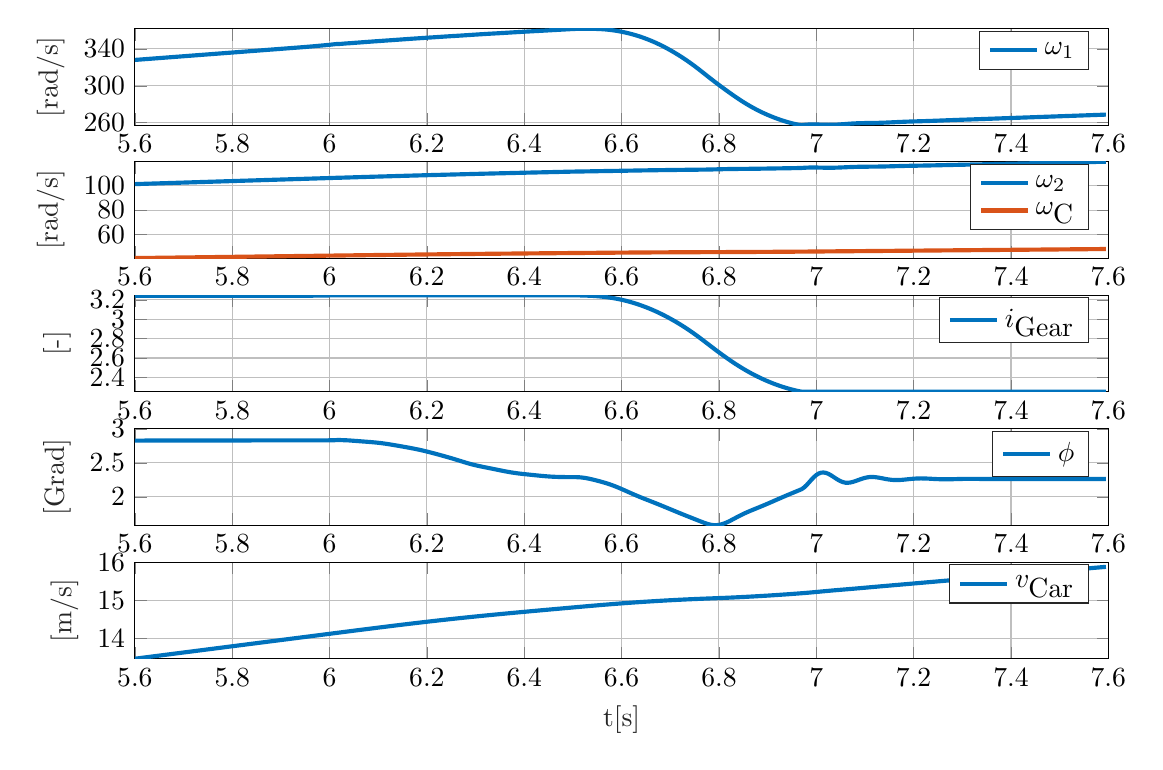
\begin{tikzpicture}

\begin{axis}[%
width=0.951\fwidth,
height=0.153\fheight,
at={(0\fwidth,0.847\fheight)},
scale only axis,
xmin=5.6,
xmax=7.6,
ymin=257.354045623529,
ymax=361.679637623739,
ytick={260,300,340,380},
ylabel style={font=\color{white!15!black}},
ylabel={[rad/s]},
axis background/.style={fill=white},
xmajorgrids,
ymajorgrids,
legend style={legend cell align=left, align=left, draw=white!15!black}
]
\addplot [color=mycolor1, line width=1.5pt]
  table[row sep=crcr]{%
5.6	327.973015972613\\
5.605	328.173196503571\\
5.61	328.373377189262\\
5.615	328.573558029248\\
5.62	328.77373902354\\
5.625	328.9739201717\\
5.63	329.17410147374\\
5.635	329.374282929225\\
5.64	329.574464538165\\
5.645	329.774646300127\\
5.65	329.974828215121\\
5.655	330.175010282715\\
5.66	330.37519250292\\
5.665	330.575374875305\\
5.67	330.775557399881\\
5.675	330.975740076218\\
5.68	331.175922904329\\
5.685	331.376105883782\\
5.69	331.576289014591\\
5.695	331.776472296327\\
5.7	331.976655729004\\
5.705	332.176839398926\\
5.71	332.377023359994\\
5.715	332.577207607051\\
5.72	332.777392092824\\
5.725	332.977576746185\\
5.73	333.177761520152\\
5.735	333.377946401713\\
5.74	333.578131405322\\
5.745	333.778316564264\\
5.75	333.978501911663\\
5.755	334.17868746763\\
5.76	334.378873242654\\
5.765	334.579059229031\\
5.77	334.779245419121\\
5.775	334.97943179968\\
5.78	335.179618366812\\
5.785	335.379805119474\\
5.79	335.579992066947\\
5.795	335.780179219412\\
5.8	335.980366594676\\
5.805	336.180554205209\\
5.81	336.380742070454\\
5.815	336.580930200169\\
5.82	336.781118613834\\
5.825	336.981307319995\\
5.83	337.181496341677\\
5.835	337.381685690897\\
5.84	337.581875399766\\
5.845	337.782065488441\\
5.85	337.982256003904\\
5.855	338.182446978476\\
5.86	338.382638480555\\
5.865	338.582830559391\\
5.87	338.783023314165\\
5.875	338.983216818814\\
5.88	339.183411218523\\
5.885	339.383606625394\\
5.89	339.583803255845\\
5.895	339.784001283118\\
5.9	339.984203437222\\
5.905	340.184423444781\\
5.91	340.384662688598\\
5.915	340.584920777348\\
5.92	340.785202123771\\
5.925	340.985519815592\\
5.93	341.186206389999\\
5.935	341.388354006297\\
5.94	341.592946524018\\
5.945	341.800935890059\\
5.95	342.013107812181\\
5.955	342.229420441504\\
5.96	342.449734053744\\
5.965	342.674934505967\\
5.97	342.905023399682\\
5.975	343.139630633068\\
5.98	343.378425455854\\
5.985	343.621540477615\\
5.99	343.867954470477\\
5.995	344.118352535604\\
6	344.372703897788\\
6.005	344.654072003652\\
6.01	344.966516209916\\
6.015	345.202428225592\\
6.02	345.262347786843\\
6.025	345.405345487616\\
6.03	345.663139985069\\
6.035	345.86931042348\\
6.04	346.023858169042\\
6.045	346.205383312853\\
6.05	346.420380257031\\
6.055	346.623722846069\\
6.06	346.813413472045\\
6.065	347.009737278534\\
6.07	347.213800688502\\
6.075	347.412748145835\\
6.08	347.605348430062\\
6.085	347.796908163182\\
6.09	347.988008802936\\
6.095	348.176093307189\\
6.1	348.360735466807\\
6.105	348.544353852605\\
6.11	348.728266935928\\
6.115	348.912424161481\\
6.12	349.096930333147\\
6.125	349.282631262076\\
6.13	349.469861139519\\
6.135	349.658283107268\\
6.14	349.847220090027\\
6.145	350.036168282051\\
6.15	350.224615339315\\
6.155	350.41184132042\\
6.16	350.597177640185\\
6.165	350.780237527707\\
6.17	350.960903795869\\
6.175	351.139232579521\\
6.18	351.315460282546\\
6.185	351.490023667203\\
6.19	351.663470234058\\
6.195	351.83631933629\\
6.2	352.009009191331\\
6.205	352.181857759664\\
6.21	352.355009170299\\
6.215	352.528398682487\\
6.22	352.701780572469\\
6.225	352.874775957789\\
6.23	353.046923886319\\
6.235	353.217736410717\\
6.24	353.386777509949\\
6.245	353.553718558233\\
6.25	353.718374705874\\
6.255	353.880429491596\\
6.26	354.041002086847\\
6.265	354.202305376821\\
6.27	354.366540001818\\
6.275	354.534641723053\\
6.28	354.705821095555\\
6.285	354.879307220587\\
6.29	355.054412681542\\
6.295	355.229925058381\\
6.3	355.403911945543\\
6.305	355.574658469269\\
6.31	355.741904114917\\
6.315	355.90488633502\\
6.32	356.063719047758\\
6.325	356.218735720006\\
6.33	356.370610140126\\
6.335	356.520388348996\\
6.34	356.669447911039\\
6.345	356.818940320103\\
6.35	356.969749937719\\
6.355	357.122493541639\\
6.36	357.277434235377\\
6.365	357.434356927307\\
6.37	357.592635532387\\
6.375	357.751435122682\\
6.38	357.909824855547\\
6.385	358.06685108315\\
6.39	358.221706286484\\
6.395	358.373874955784\\
6.4	358.523179234926\\
6.405	358.669778566807\\
6.41	358.814130628351\\
6.415	358.956942510867\\
6.42	359.099051843604\\
6.425	359.241298818347\\
6.43	359.384404482048\\
6.435	359.528896021368\\
6.44	359.675029853693\\
6.445	359.822774231398\\
6.45	359.971826637323\\
6.455	360.121680758037\\
6.46	360.271707493666\\
6.465	360.421251790185\\
6.47	360.569731678366\\
6.475	360.716723821903\\
6.48	360.862017644565\\
6.485	361.005639606492\\
6.49	361.14784167151\\
6.495	361.289059269372\\
6.5	361.429841566652\\
6.505	361.541963908227\\
6.51	361.609776061552\\
6.515	361.648421634541\\
6.52	361.669859428241\\
6.525	361.679637623739\\
6.53	361.679557373908\\
6.535	361.667668276279\\
6.54	361.63951111462\\
6.545	361.589004233596\\
6.55	361.51100234488\\
6.555	361.4002673758\\
6.56	361.251659202263\\
6.565	361.061522138762\\
6.57	360.827447907499\\
6.575	360.548123458717\\
6.58	360.22323881264\\
6.585	359.853096907383\\
6.59	359.438356285236\\
6.595	358.979737076568\\
6.6	358.477805196846\\
6.605	357.932795002571\\
6.61	357.344525811013\\
6.615	356.712407266668\\
6.62	356.035492617687\\
6.625	355.312594680318\\
6.63	354.542420530599\\
6.635	353.723715194602\\
6.64	352.855392726343\\
6.645	351.936635720995\\
6.65	350.966954412869\\
6.655	349.946200322662\\
6.66	348.874546816889\\
6.665	347.752423751474\\
6.67	346.580441473408\\
6.675	345.359291968297\\
6.68	344.089657474189\\
6.685	342.7721306054\\
6.69	341.4071534845\\
6.695	339.994983491629\\
6.7	338.535685530385\\
6.705	337.029147201719\\
6.71	335.475115179975\\
6.715	333.873245388733\\
6.72	332.223155302155\\
6.725	330.524474153146\\
6.73	328.77689168388\\
6.735	326.980187747693\\
6.74	325.134248819561\\
6.745	323.239066563037\\
6.75	321.294731529412\\
6.755	319.298439369855\\
6.76	317.262759463327\\
6.765	315.195513677176\\
6.77	313.111049203975\\
6.775	311.024463046329\\
6.78	308.947973351847\\
6.785	306.892958231272\\
6.79	304.864661964201\\
6.795	302.862130393347\\
6.8	300.883847836708\\
6.805	298.927676314899\\
6.81	296.992189418147\\
6.815	295.07672570102\\
6.82	293.182041972211\\
6.825	291.310387845389\\
6.83	289.465405433905\\
6.835	287.651724793431\\
6.84	285.874546537157\\
6.845	284.139068939194\\
6.85	282.450083471727\\
6.855	280.811524975373\\
6.86	279.226308696731\\
6.865	277.696148626036\\
6.87	276.221686650797\\
6.875	274.802555770197\\
6.88	273.437704078713\\
6.885	272.12557378135\\
6.89	270.864463934088\\
6.895	269.652682042429\\
6.9	268.488819107188\\
6.905	267.371785690578\\
6.91	266.300949687745\\
6.915	265.276046067966\\
6.92	264.297202295732\\
6.925	263.364768502307\\
6.93	262.479295064637\\
6.935	261.641348353161\\
6.94	260.851503415411\\
6.945	260.110194292244\\
6.95	259.417756304875\\
6.955	258.77432782773\\
6.96	258.179942889167\\
6.965	257.634472783561\\
6.97	257.354045623529\\
6.975	257.6646046711\\
6.98	257.903029942911\\
6.985	258.064783741053\\
6.99	258.141902522297\\
6.995	258.145997000496\\
7	258.103737849351\\
7.005	258.021335486802\\
7.01	257.925505249587\\
7.015	257.835165164343\\
7.02	257.766399541142\\
7.025	257.73087162692\\
7.03	257.738248881135\\
7.035	257.793174080001\\
7.04	257.894781899613\\
7.045	258.040477496337\\
7.05	258.21755673364\\
7.055	258.41433640153\\
7.06	258.620342801915\\
7.065	258.821672656543\\
7.07	259.011795814309\\
7.075	259.176839380176\\
7.08	259.31636097511\\
7.085	259.431120391346\\
7.09	259.519689621202\\
7.095	259.587291871016\\
7.1	259.639671663221\\
7.105	259.679762592514\\
7.11	259.713571589958\\
7.115	259.74814750626\\
7.12	259.791616257467\\
7.125	259.84664746329\\
7.13	259.914453615949\\
7.135	259.996656549938\\
7.14	260.091701537962\\
7.145	260.198941643773\\
7.15	260.315505245924\\
7.155	260.438631583401\\
7.16	260.564762565458\\
7.165	260.69002824374\\
7.17	260.812210189362\\
7.175	260.928923306729\\
7.18	261.038416097178\\
7.185	261.140171785139\\
7.19	261.234353827565\\
7.195	261.32168017479\\
7.2	261.403895198407\\
7.205	261.482869309665\\
7.21	261.560083457766\\
7.215	261.637101122048\\
7.22	261.715859598331\\
7.225	261.797604011416\\
7.23	261.883237558214\\
7.235	261.973155149336\\
7.24	262.067038856012\\
7.245	262.164687254383\\
7.25	262.265118623285\\
7.255	262.36726509506\\
7.26	262.470245621921\\
7.265	262.573187511688\\
7.27	262.675383659262\\
7.275	262.776133623499\\
7.28	262.874967284262\\
7.285	262.971583336586\\
7.29	263.066080777457\\
7.295	263.15879538407\\
7.3	263.249938851468\\
7.305	263.339978157013\\
7.31	263.42944027341\\
7.315	263.518876463882\\
7.32	263.60864789009\\
7.325	263.699278212111\\
7.33	263.790892127959\\
7.335	263.883521679553\\
7.34	263.977241506976\\
7.345	264.07189149822\\
7.35	264.167375686094\\
7.355	264.263463078194\\
7.36	264.359894256678\\
7.365	264.456397986991\\
7.37	264.552755758444\\
7.375	264.648736536723\\
7.38	264.744199017935\\
7.385	264.839102168345\\
7.39	264.933369224665\\
7.395	265.027121862653\\
7.4	265.120463901962\\
7.405	265.21348092786\\
7.41	265.306313184156\\
7.415	265.399081626459\\
7.42	265.491923552198\\
7.425	265.584939621357\\
7.43	265.67820278439\\
7.435	265.771753283947\\
7.44	265.865599802397\\
7.445	265.959721790524\\
7.45	266.054075696227\\
7.455	266.148601119166\\
7.46	266.243229135219\\
7.465	266.337889275918\\
7.47	266.432515821557\\
7.475	266.527055322531\\
7.48	266.621468228581\\
7.485	266.715731309006\\
7.49	266.80983769707\\
7.495	266.903795887061\\
7.5	266.997626644955\\
7.505	267.091359964407\\
7.51	267.185030795659\\
7.515	267.278675455565\\
7.52	267.37232826575\\
7.525	267.466017705013\\
7.53	267.559765227779\\
7.535	267.653584081963\\
7.54	267.747478983114\\
7.545	267.841446671469\\
7.55	267.935477348545\\
7.555	268.029556188752\\
7.56	268.123665514973\\
7.565	268.217786660489\\
7.57	268.311901749767\\
7.575	268.405995637223\\
7.58	268.500056427535\\
7.585	268.594077211152\\
7.59	268.688054694745\\
7.595	268.781989973118\\
};
\addlegendentry{$\omega_1$}

\end{axis}

\begin{axis}[%
width=0.951\fwidth,
height=0.153\fheight,
at={(0\fwidth,0.636\fheight)},
scale only axis,
xmin=5.6,
xmax=7.6,
ymin=40.9411242903612,
ymax=119.339202965924,
ylabel style={font=\color{white!15!black}},
ylabel={[rad/s]},
axis background/.style={fill=white},
xmajorgrids,
ymajorgrids,
legend style={legend cell align=left, align=left, draw=white!15!black}
]
\addplot [color=mycolor1, line width=1.5pt]
  table[row sep=crcr]{%
5.6	101.125007147652\\
5.605	101.186729473195\\
5.61	101.248451846443\\
5.615	101.31017426726\\
5.62	101.37189673565\\
5.625	101.433619251479\\
5.63	101.495341814749\\
5.635	101.557064425326\\
5.64	101.618787083214\\
5.645	101.680509788279\\
5.65	101.742232540525\\
5.655	101.803955339817\\
5.66	101.86567818616\\
5.665	101.927401079421\\
5.67	101.989124019602\\
5.675	102.050847006571\\
5.68	102.112570040333\\
5.685	102.174293120754\\
5.69	102.236016247838\\
5.695	102.297739421453\\
5.7	102.359462641603\\
5.705	102.421185908074\\
5.71	102.482909220071\\
5.715	102.544632578056\\
5.72	102.606355982476\\
5.725	102.668079433622\\
5.73	102.729802931708\\
5.735	102.791526476543\\
5.74	102.853250067852\\
5.745	102.914973705119\\
5.75	102.97669738799\\
5.755	103.03842111609\\
5.76	103.100144889331\\
5.765	103.161868707638\\
5.77	103.223592571168\\
5.775	103.285316479997\\
5.78	103.347040434327\\
5.785	103.408764434193\\
5.79	103.470488479705\\
5.795	103.532212570776\\
5.8	103.593936707401\\
5.805	103.655660889398\\
5.81	103.717385116688\\
5.815	103.779109389052\\
5.82	103.840833706395\\
5.825	103.902558068505\\
5.83	103.964282475313\\
5.835	104.026006926642\\
5.84	104.087731422463\\
5.845	104.149455962642\\
5.85	104.211180547183\\
5.855	104.272905175977\\
5.86	104.334629849031\\
5.865	104.396354566232\\
5.87	104.458079327552\\
5.875	104.519804132832\\
5.88	104.581528981973\\
5.885	104.643253874739\\
5.89	104.704978810926\\
5.895	104.766703790199\\
5.9	104.828428789337\\
5.905	104.890153768952\\
5.91	104.95187873951\\
5.915	105.013603726045\\
5.92	105.075328734922\\
5.925	105.137053737031\\
5.93	105.198776796748\\
5.935	105.260494084285\\
5.94	105.322202949905\\
5.945	105.38390226131\\
5.95	105.44559332003\\
5.955	105.507282739061\\
5.96	105.568975336429\\
5.965	105.630673398631\\
5.97	105.692380724001\\
5.975	105.754101294427\\
5.98	105.815836390854\\
5.985	105.877585390569\\
5.99	105.939344141712\\
5.995	106.001104189957\\
6	106.062860845193\\
6.005	106.129724102794\\
6.01	106.202810983133\\
6.015	106.26554771556\\
6.02	106.304124860576\\
6.025	106.35523051389\\
6.03	106.422768108335\\
6.035	106.482963772158\\
6.04	106.536272943804\\
6.045	106.594060195641\\
6.05	106.656998434327\\
6.055	106.718547792258\\
6.06	106.778401050756\\
6.065	106.839320773136\\
6.07	106.901245990124\\
6.075	106.962177626277\\
6.08	107.021846026197\\
6.085	107.080944342386\\
6.09	107.139527533129\\
6.095	107.197258170539\\
6.1	107.254170534149\\
6.105	107.31072698077\\
6.11	107.367233040934\\
6.115	107.423804362989\\
6.12	107.480558325796\\
6.125	107.53767845392\\
6.13	107.595225256735\\
6.135	107.653125596235\\
6.14	107.711211970049\\
6.145	107.769316364396\\
6.15	107.827260194229\\
6.155	107.884825900539\\
6.16	107.941823104253\\
6.165	107.998129570897\\
6.17	108.053697064356\\
6.175	108.108541736444\\
6.18	108.162740510035\\
6.185	108.216424850021\\
6.19	108.269757872043\\
6.195	108.322899954839\\
6.2	108.375988624147\\
6.205	108.429122074188\\
6.21	108.482344928085\\
6.215	108.535639622339\\
6.22	108.588933148184\\
6.225	108.642110258357\\
6.23	108.69502976777\\
6.235	108.74754220948\\
6.24	108.799513515842\\
6.245	108.850841606493\\
6.25	108.901468159609\\
6.255	108.951375608022\\
6.26	109.001035747863\\
6.265	109.051007140532\\
6.27	109.101812941741\\
6.275	109.153705059323\\
6.28	109.206575669072\\
6.285	109.260214173136\\
6.29	109.314345058035\\
6.295	109.368578008481\\
6.3	109.422359958746\\
6.305	109.475168523129\\
6.31	109.52692868278\\
6.315	109.57739308811\\
6.32	109.626560194387\\
6.325	109.674538785646\\
6.33	109.721557141208\\
6.335	109.767932117531\\
6.34	109.814065393667\\
6.345	109.860310608902\\
6.35	109.906955643148\\
6.355	109.954194906623\\
6.36	110.002101832767\\
6.365	110.050614480975\\
6.37	110.09955153244\\
6.375	110.148659120263\\
6.38	110.197647434745\\
6.385	110.246223874464\\
6.39	110.294142529277\\
6.395	110.341242069495\\
6.4	110.387462315614\\
6.405	110.432849215471\\
6.41	110.477541974148\\
6.415	110.521755198931\\
6.42	110.565743529142\\
6.425	110.609765435687\\
6.43	110.654044191643\\
6.435	110.698743417552\\
6.44	110.743943978421\\
6.445	110.789639170895\\
6.45	110.835739077627\\
6.455	110.882090122234\\
6.46	110.92850011738\\
6.465	110.974768276795\\
6.47	111.020715345303\\
6.475	111.066209744819\\
6.48	111.111184650463\\
6.485	111.155645950741\\
6.49	111.199668919346\\
6.495	111.243385484008\\
6.5	111.286963148873\\
6.505	111.326476010501\\
6.51	111.3599364749\\
6.515	111.390154293476\\
6.52	111.419741233839\\
6.525	111.450311102238\\
6.53	111.482819532196\\
6.535	111.517448126501\\
6.54	111.553821817973\\
6.545	111.591274978874\\
6.55	111.629008619738\\
6.555	111.66634434016\\
6.56	111.702695430614\\
6.565	111.737726454786\\
6.57	111.77136417231\\
6.575	111.803764304814\\
6.58	111.835280627755\\
6.585	111.866367169053\\
6.59	111.897506753115\\
6.595	111.929134794622\\
6.6	111.961585527127\\
6.605	111.995044905989\\
6.61	112.029537502262\\
6.615	112.064935705314\\
6.62	112.100982428715\\
6.625	112.137332485927\\
6.63	112.173598099124\\
6.635	112.209396106882\\
6.64	112.244390766456\\
6.645	112.278325915668\\
6.65	112.311044339041\\
6.655	112.342492821579\\
6.66	112.372716829559\\
6.665	112.40184096554\\
6.67	112.430046083051\\
6.675	112.457539308418\\
6.68	112.484526275687\\
6.685	112.511186790495\\
6.69	112.537656214437\\
6.695	112.564014854442\\
6.7	112.59028534479\\
6.705	112.61643693141\\
6.71	112.6423961464\\
6.715	112.66806167188\\
6.72	112.693319901151\\
6.725	112.71805984268\\
6.73	112.742187753337\\
6.735	112.765636049422\\
6.74	112.788368367548\\
6.745	112.810379316502\\
6.75	112.831692773247\\
6.755	112.852423364193\\
6.76	112.873411817625\\
6.765	112.896199019225\\
6.77	112.922640853486\\
6.775	112.954375334299\\
6.78	112.992271088282\\
6.785	113.036795927066\\
6.79	113.086522659965\\
6.795	113.139059378772\\
6.8	113.192160745349\\
6.805	113.243695590131\\
6.81	113.291841553258\\
6.815	113.335258816879\\
6.82	113.373207856742\\
6.825	113.405570999167\\
6.83	113.432786581897\\
6.835	113.455735661682\\
6.84	113.475582577112\\
6.845	113.493614378466\\
6.85	113.51108386661\\
6.855	113.529084806782\\
6.86	113.548464650577\\
6.865	113.56977803994\\
6.87	113.59328597027\\
6.875	113.618982794927\\
6.88	113.646656018657\\
6.885	113.675951438021\\
6.89	113.706449751767\\
6.895	113.737729119123\\
6.9	113.769421665048\\
6.905	113.801247000694\\
6.91	113.833032493383\\
6.915	113.864712523507\\
6.92	113.896317391505\\
6.925	113.927949611462\\
6.93	113.959758215272\\
6.935	113.991909459852\\
6.94	114.024563860449\\
6.945	114.057855122089\\
6.95	114.091880039321\\
6.955	114.126691072802\\
6.96	114.162300090754\\
6.965	114.198682134972\\
6.97	114.266609097247\\
6.975	114.401900087165\\
6.98	114.507622908556\\
6.985	114.579462774693\\
6.99	114.613846427011\\
6.995	114.615897406591\\
7	114.597422027448\\
7.005	114.561160589861\\
7.01	114.518935121215\\
7.015	114.479101496988\\
7.02	114.448792203667\\
7.025	114.433172888353\\
7.03	114.4365256406\\
7.035	114.460911746963\\
7.04	114.505954627114\\
7.045	114.57051412835\\
7.05	114.648967566754\\
7.055	114.736156322101\\
7.06	114.827482859476\\
7.065	114.916746058485\\
7.07	115.000946450715\\
7.075	115.074141246801\\
7.08	115.136049335774\\
7.085	115.187003642974\\
7.09	115.226368949758\\
7.095	115.256453731438\\
7.1	115.279798546699\\
7.105	115.297699312311\\
7.11	115.3128128689\\
7.115	115.328253991684\\
7.12	115.34762648973\\
7.125	115.372105573629\\
7.13	115.402235295555\\
7.135	115.438734311803\\
7.14	115.480915961417\\
7.145	115.528495210596\\
7.15	115.5802029189\\
7.155	115.634818364004\\
7.16	115.690767821117\\
7.165	115.746337703065\\
7.17	115.800546519914\\
7.175	115.85233856845\\
7.18	115.900938094332\\
7.185	115.946115329721\\
7.19	115.987941577259\\
7.195	116.026733535567\\
7.2	116.063262328393\\
7.205	116.098355301459\\
7.21	116.132667512697\\
7.215	116.166890038329\\
7.22	116.201880464872\\
7.225	116.238190512207\\
7.23	116.276220274566\\
7.235	116.316145046464\\
7.24	116.357824805545\\
7.245	116.401170872887\\
7.25	116.445749208164\\
7.255	116.491087545986\\
7.26	116.536795988522\\
7.265	116.582488364397\\
7.27	116.627851686549\\
7.275	116.672576016059\\
7.28	116.716453104724\\
7.285	116.759349345762\\
7.29	116.801308236162\\
7.295	116.842478121671\\
7.3	116.882952452087\\
7.305	116.922937688485\\
7.31	116.962666886091\\
7.315	117.002384126038\\
7.32	117.042248323005\\
7.325	117.082493462558\\
7.33	117.123172294924\\
7.335	117.164300512469\\
7.34	117.205911430366\\
7.345	117.247933920366\\
7.35	117.290325672709\\
7.355	117.332984614103\\
7.36	117.375795975168\\
7.365	117.418639740572\\
7.37	117.461419154829\\
7.375	117.504032039408\\
7.38	117.546415789631\\
7.385	117.588552165856\\
7.39	117.630407123191\\
7.395	117.672034422968\\
7.4	117.713479957661\\
7.405	117.754781543203\\
7.41	117.796001220426\\
7.415	117.837192486132\\
7.42	117.878416030506\\
7.425	117.919716546843\\
7.43	117.961126271494\\
7.435	118.002663068984\\
7.44	118.044330828333\\
7.445	118.086120488222\\
7.45	118.128012808234\\
7.455	118.169981085287\\
7.46	118.211994835101\\
7.465	118.254022880697\\
7.47	118.296036116832\\
7.475	118.338010910015\\
7.48	118.379929741004\\
7.485	118.421782311651\\
7.49	118.463565563134\\
7.495	118.505283234351\\
7.5	118.546944496705\\
7.505	118.588562608483\\
7.51	118.630153025712\\
7.515	118.671731813984\\
7.52	118.713314139188\\
7.525	118.75491265078\\
7.53	118.796536831272\\
7.535	118.838192538558\\
7.54	118.879881884831\\
7.545	118.921603436346\\
7.55	118.96335286398\\
7.555	119.005123614811\\
7.56	119.046907871546\\
7.565	119.088697376176\\
7.57	119.130484212864\\
7.575	119.172261684971\\
7.58	119.214024524552\\
7.585	119.255769669299\\
7.59	119.297495656703\\
7.595	119.339202965924\\
};
\addlegendentry{$\omega_2$}

\addplot [color=mycolor2, line width=1.5pt]
  table[row sep=crcr]{%
5.6	40.9411242903612\\
5.605	40.9661130055681\\
5.61	40.9911017400735\\
5.615	41.0160904938306\\
5.62	41.0410792668329\\
5.625	41.0660680590339\\
5.63	41.0910568704269\\
5.635	41.1160457009657\\
5.64	41.1410345506436\\
5.645	41.1660234194145\\
5.65	41.1910123072718\\
5.655	41.2160012141695\\
5.66	41.2409901401011\\
5.665	41.2659790850206\\
5.67	41.2909680489216\\
5.675	41.3159570317583\\
5.68	41.3409460335243\\
5.685	41.3659350541739\\
5.69	41.3909240937008\\
5.695	41.4159131520595\\
5.7	41.4409022292435\\
5.705	41.4658913253713\\
5.71	41.4908804401125\\
5.715	41.5158695735735\\
5.72	41.5408587257498\\
5.725	41.5658478965957\\
5.73	41.5908370861058\\
5.735	41.6158262942373\\
5.74	41.6408155209869\\
5.745	41.6658047663126\\
5.75	41.6907940302103\\
5.755	41.7157833126364\\
5.76	41.7407726135845\\
5.765	41.7657619330088\\
5.77	41.7907512709015\\
5.775	41.8157406272159\\
5.78	41.840730001944\\
5.785	41.8657193950399\\
5.79	41.8907088064963\\
5.795	41.9156982362685\\
5.8	41.9406876843503\\
5.805	41.9656771506982\\
5.81	41.9906666353064\\
5.815	42.0156561381318\\
5.82	42.0406456591687\\
5.825	42.0656351983738\\
5.83	42.0906247557408\\
5.835	42.1156143312256\\
5.84	42.1406039248211\\
5.845	42.1655935364824\\
5.85	42.1905831662016\\
5.855	42.215572813933\\
5.86	42.2405624796678\\
5.865	42.2655521633599\\
5.87	42.2905418649998\\
5.875	42.3155315845406\\
5.88	42.3405213219719\\
5.885	42.3655110772456\\
5.89	42.3905008503493\\
5.895	42.4154906412326\\
5.9	42.4404804484467\\
5.905	42.4654702718395\\
5.91	42.4904601125349\\
5.915	42.5154499702278\\
5.92	42.5404398445983\\
5.925	42.5654297352734\\
5.93	42.59041964069\\
5.935	42.6154095491356\\
5.94	42.640399436242\\
5.945	42.6653892613233\\
5.95	42.6903789679894\\
5.955	42.7153684943565\\
5.96	42.7403577872581\\
5.965	42.765346804387\\
5.97	42.7903355188569\\
5.975	42.8153239259309\\
5.98	42.840312048524\\
5.985	42.8652999207335\\
5.99	42.8902876372471\\
5.995	42.9152752590089\\
6	42.9402628475297\\
6.005	42.9652542352751\\
6.01	42.9902689040836\\
6.015	43.0153250690856\\
6.02	43.0403820478348\\
6.025	43.0654002350553\\
6.03	43.0903922301533\\
6.035	43.1153709622979\\
6.04	43.1403189186165\\
6.045	43.1652223312713\\
6.05	43.1900859698959\\
6.055	43.2149147790135\\
6.06	43.2397051497686\\
6.065	43.2644550906679\\
6.07	43.2891665079372\\
6.075	43.3138406637853\\
6.08	43.3384754745209\\
6.085	43.3630678316204\\
6.09	43.3876145561358\\
6.095	43.412111443738\\
6.1	43.4365524762989\\
6.105	43.4609314890439\\
6.11	43.4852428664018\\
6.115	43.5094810351788\\
6.12	43.5336411012665\\
6.125	43.5577190639003\\
6.13	43.5817122533054\\
6.135	43.6056189454089\\
6.14	43.6294378866308\\
6.145	43.6531683840006\\
6.15	43.676809843469\\
6.155	43.7003613982746\\
6.16	43.7238216351673\\
6.165	43.7471883308505\\
6.17	43.7704584239108\\
6.175	43.7936280126664\\
6.18	43.816692534301\\
6.185	43.8396470099513\\
6.19	43.862486316969\\
6.195	43.8852055146739\\
6.2	43.9078000981977\\
6.205	43.9302661810867\\
6.21	43.952600578795\\
6.215	43.974800816927\\
6.22	43.9968649977123\\
6.225	44.0187916059883\\
6.23	44.0405792840095\\
6.235	44.0622265881143\\
6.24	44.0837317454525\\
6.245	44.1050924950499\\
6.25	44.1263059965551\\
6.255	44.1473541320612\\
6.26	44.1682413956052\\
6.265	44.188990988516\\
6.27	44.2095853467352\\
6.275	44.2300248505961\\
6.28	44.250314078508\\
6.285	44.2704597564578\\
6.29	44.2904697046318\\
6.295	44.3103520935165\\
6.3	44.3301093421615\\
6.305	44.3497489298223\\
6.31	44.3692960201456\\
6.315	44.3887415334117\\
6.32	44.4080873533404\\
6.325	44.4273341876994\\
6.33	44.4464814128407\\
6.335	44.4655278358783\\
6.34	44.4844721116632\\
6.345	44.503313554719\\
6.35	44.5220525646704\\
6.355	44.5406909241674\\
6.36	44.5592320672781\\
6.365	44.5776808355189\\
6.37	44.5960431949066\\
6.375	44.6143257335168\\
6.38	44.6325351727676\\
6.385	44.650677838504\\
6.39	44.6687591807301\\
6.395	44.6867834838203\\
6.4	44.7047537696405\\
6.405	44.7226718197495\\
6.41	44.740538453099\\
6.415	44.7583538607979\\
6.42	44.7761180505916\\
6.425	44.7938312785727\\
6.43	44.8114944694323\\
6.435	44.8291094460848\\
6.44	44.8466791061615\\
6.445	44.8642073614784\\
6.45	44.8816989945291\\
6.455	44.8991593567883\\
6.46	44.9165940210365\\
6.465	44.9340084126451\\
6.47	44.9514074788455\\
6.475	44.9687954380736\\
6.48	44.98617565278\\
6.485	45.0035506190236\\
6.49	45.0209220901195\\
6.495	45.0382912967647\\
6.5	45.0556592326757\\
6.505	45.0730237872153\\
6.51	45.0903700604269\\
6.515	45.1076749342648\\
6.52	45.1249163040754\\
6.525	45.1420746576751\\
6.53	45.1591333156477\\
6.535	45.1760803333087\\
6.54	45.1929074877429\\
6.545	45.209606723452\\
6.55	45.2261772135695\\
6.555	45.2426141035564\\
6.56	45.2589101678486\\
6.565	45.275057657124\\
6.57	45.2910470772889\\
6.575	45.3068675019391\\
6.58	45.3225070743761\\
6.585	45.3379539996635\\
6.59	45.3531973866107\\
6.595	45.3682280427852\\
6.6	45.3830389895028\\
6.605	45.3976259685769\\
6.61	45.4119874133372\\
6.615	45.4261242049074\\
6.62	45.4400392703979\\
6.625	45.4537369442244\\
6.63	45.46722230167\\
6.635	45.4805004879603\\
6.64	45.4935761134689\\
6.645	45.5064528047892\\
6.65	45.519132929978\\
6.655	45.5316175174647\\
6.66	45.5439063147434\\
6.665	45.555998035159\\
6.67	45.5678906499513\\
6.675	45.5795817738044\\
6.68	45.5910690225104\\
6.685	45.6023503270298\\
6.69	45.6134241742035\\
6.695	45.624289745094\\
6.7	45.6349469510514\\
6.705	45.6453963816173\\
6.71	45.6556391709919\\
6.715	45.6656768110274\\
6.72	45.6755109550731\\
6.725	45.6851432305566\\
6.73	45.6945750538637\\
6.735	45.7038075176153\\
6.74	45.7128413260738\\
6.745	45.7216767970093\\
6.75	45.7303138818124\\
6.755	45.7387369587049\\
6.76	45.746976865704\\
6.765	45.7550227321265\\
6.77	45.7628844420224\\
6.775	45.7705825241749\\
6.78	45.7781474199802\\
6.785	45.7856176179394\\
6.79	45.793058602672\\
6.795	45.800535191317\\
6.8	45.8081050697241\\
6.805	45.8158197396308\\
6.81	45.8237251377708\\
6.815	45.8318570495616\\
6.82	45.8402407673786\\
6.825	45.8488908482278\\
6.83	45.8578125190732\\
6.835	45.8670030259277\\
6.84	45.8764542076791\\
6.845	45.8861543812258\\
6.85	45.8960908906542\\
6.855	45.9062515330852\\
6.86	45.9166262523683\\
6.865	45.9272075907856\\
6.87	45.9379913019808\\
6.875	45.9489758701538\\
6.88	45.9601623288739\\
6.885	45.9715532552354\\
6.89	45.9831523078709\\
6.895	45.9949631797664\\
6.9	46.0069893040462\\
6.905	46.0192330958139\\
6.91	46.0316960413844\\
6.915	46.0443783180349\\
6.92	46.0572792377091\\
6.925	46.0703971375588\\
6.93	46.083730002421\\
6.935	46.0972754378438\\
6.94	46.1110312769479\\
6.945	46.1249954770933\\
6.95	46.1391665900231\\
6.955	46.1535435122805\\
6.96	46.1681257988004\\
6.965	46.1829132859708\\
6.97	46.1979119135764\\
6.975	46.2133046709661\\
6.98	46.2292295290931\\
6.985	46.2457367346182\\
6.99	46.2628693147068\\
6.995	46.2805301684145\\
7	46.2985213178138\\
7.005	46.3167932129136\\
7.01	46.335153149845\\
7.015	46.3534646402439\\
7.02	46.3716124058533\\
7.025	46.3895129099247\\
7.03	46.4070967355262\\
7.035	46.4243310860751\\
7.04	46.4412230279886\\
7.045	46.4577918581975\\
7.05	46.4741308174776\\
7.055	46.4903251246984\\
7.06	46.5064503265645\\
7.065	46.5226089496622\\
7.07	46.5388515958738\\
7.075	46.5552742763651\\
7.08	46.5718823517847\\
7.085	46.5886703382331\\
7.09	46.605648592878\\
7.095	46.6227791053669\\
7.1	46.6400200688761\\
7.105	46.657350043983\\
7.11	46.6747252606248\\
7.115	46.6920943873386\\
7.12	46.7093979850213\\
7.125	46.7266169047055\\
7.13	46.7437422016576\\
7.135	46.7607620386893\\
7.14	46.7776877951033\\
7.145	46.7945241559011\\
7.15	46.811292059058\\
7.155	46.828011605638\\
7.16	46.8447086797363\\
7.165	46.8614115449014\\
7.17	46.8781363995385\\
7.175	46.894900580142\\
7.18	46.9117168294387\\
7.185	46.9285889246781\\
7.19	46.9455156732095\\
7.195	46.9624918231687\\
7.2	46.9795046822432\\
7.205	46.996540667782\\
7.21	47.0135889930251\\
7.215	47.0306382048572\\
7.22	47.04767416927\\
7.225	47.0646878394685\\
7.23	47.0816726247932\\
7.235	47.0986256434948\\
7.24	47.1155492375393\\
7.245	47.132444829532\\
7.25	47.1493195908924\\
7.255	47.166181327328\\
7.26	47.1830364879446\\
7.265	47.1998913926714\\
7.27	47.2167512380131\\
7.275	47.2336210869098\\
7.28	47.2505043628191\\
7.285	47.2674032412752\\
7.29	47.2843170186298\\
7.295	47.3012432876379\\
7.3	47.3181804683423\\
7.305	47.3351251559328\\
7.31	47.3520734842045\\
7.315	47.3690214589187\\
7.32	47.3859665237685\\
7.325	47.4029046861749\\
7.33	47.4198351810921\\
7.335	47.4367577685003\\
7.34	47.4536718637671\\
7.345	47.4705786833251\\
7.35	47.4874788884416\\
7.355	47.5043741617505\\
7.36	47.5212663902731\\
7.365	47.5381575452234\\
7.37	47.5550492588191\\
7.375	47.5719431540244\\
7.38	47.5888402752424\\
7.385	47.6057409505847\\
7.39	47.6226456710918\\
7.395	47.6395536097902\\
7.4	47.6564640388938\\
7.405	47.6733762923031\\
7.41	47.690289387053\\
7.415	47.7072024023386\\
7.42	47.7241143216818\\
7.425	47.7410244376314\\
7.43	47.7579322156263\\
7.435	47.7748373621179\\
7.44	47.7917398131076\\
7.445	47.8086397187543\\
7.45	47.8255373959065\\
7.455	47.8424332850009\\
7.46	47.8593278877788\\
7.465	47.876221718052\\
7.47	47.8931152470475\\
7.475	47.910008878472\\
7.48	47.9269028937679\\
7.485	47.943797461812\\
7.49	47.9606926320692\\
7.495	47.977588342909\\
7.5	47.9944844424579\\
7.505	48.0113807124252\\
7.51	48.0282768975796\\
7.515	48.0451727335552\\
7.52	48.0620679625051\\
7.525	48.0789623908453\\
7.53	48.0958558558242\\
7.535	48.1127482608206\\
7.54	48.1296395705433\\
7.545	48.1465298090518\\
7.55	48.1634190472506\\
7.555	48.1803073934423\\
7.56	48.1971949758907\\
7.565	48.2140819309038\\
7.57	48.2309683806183\\
7.575	48.2478544502185\\
7.58	48.2647402151191\\
7.585	48.2816257339652\\
7.59	48.298511025996\\
7.595	48.315396083398\\
};
\addlegendentry{$\omega_\textrm{C}$}

\end{axis}

\begin{axis}[%
width=0.951\fwidth,
height=0.153\fheight,
at={(0\fwidth,0.424\fheight)},
scale only axis,
xmin=5.6,
xmax=7.6,
ymin=2.25222440445841,
ymax=3.24848867433114,
ylabel style={font=\color{white!15!black}},
ylabel={[-]},
axis background/.style={fill=white},
xmajorgrids,
ymajorgrids,
legend style={legend cell align=left, align=left, draw=white!15!black}
]
\addplot [color=mycolor1, line width=1.5pt]
  table[row sep=crcr]{%
5.6	3.24324343921916\\
5.605	3.24324343925461\\
5.61	3.24324343929017\\
5.615	3.24324343932583\\
5.62	3.24324343936161\\
5.625	3.24324343939748\\
5.63	3.24324343943347\\
5.635	3.24324343946955\\
5.64	3.24324343950574\\
5.645	3.24324343954203\\
5.65	3.24324343957844\\
5.655	3.24324343961493\\
5.66	3.24324343965155\\
5.665	3.24324343968826\\
5.67	3.24324343972508\\
5.675	3.243243439762\\
5.68	3.24324343979904\\
5.685	3.24324343983617\\
5.69	3.24324343987341\\
5.695	3.24324343991075\\
5.7	3.24324343994821\\
5.705	3.24324344083522\\
5.71	3.24324344312134\\
5.715	3.24324344673913\\
5.72	3.24324345121134\\
5.725	3.24324345583444\\
5.73	3.24324346014406\\
5.735	3.24324346402026\\
5.74	3.24324346761296\\
5.745	3.24324347126234\\
5.75	3.24324347530118\\
5.755	3.24324347993571\\
5.76	3.2432434852694\\
5.765	3.24324349122864\\
5.77	3.2432434977334\\
5.775	3.24324350465204\\
5.78	3.24324351193981\\
5.785	3.24324351958485\\
5.79	3.24324352767282\\
5.795	3.2432435363039\\
5.8	3.24324354564927\\
5.805	3.24324355583357\\
5.81	3.24324356704526\\
5.815	3.24324357938339\\
5.82	3.2432435930365\\
5.825	3.2432436080911\\
5.83	3.24324362476838\\
5.835	3.2432436431864\\
5.84	3.24324366365155\\
5.845	3.24324368635781\\
5.85	3.24324371175201\\
5.855	3.24324374014266\\
5.86	3.2432437721798\\
5.865	3.24324380833226\\
5.87	3.24324384954308\\
5.875	3.24324389651562\\
5.88	3.24324395063099\\
5.885	3.24324401295517\\
5.89	3.24324408554686\\
5.895	3.24324417005192\\
5.9	3.24324429321034\\
5.905	3.24324458703843\\
5.91	3.24324506408723\\
5.915	3.24324571953411\\
5.92	3.24324659486419\\
5.925	3.24324781507065\\
5.93	3.24325260025784\\
5.935	3.24327143793319\\
5.94	3.24331372641808\\
5.945	3.2433884925093\\
5.95	3.24350309049107\\
5.955	3.24365685056927\\
5.96	3.24384823251735\\
5.965	3.2440854865402\\
5.97	3.24436843082497\\
5.975	3.24469336350125\\
5.98	3.24505704597477\\
5.985	3.24546068188124\\
5.99	3.24589468866727\\
5.995	3.24636573519964\\
6	3.24687361017376\\
6.005	3.24747920450476\\
6.01	3.24818630520713\\
6.015	3.24848867433114\\
6.02	3.24787347847201\\
6.025	3.24765734434195\\
6.03	3.24801869119957\\
6.035	3.24811874285861\\
6.04	3.2479440908503\\
6.045	3.2478862581783\\
6.05	3.24798546126662\\
6.055	3.248017612841\\
6.06	3.24797346709838\\
6.065	3.24795903575031\\
6.07	3.24798647080857\\
6.075	3.24799621563135\\
6.08	3.24798498004767\\
6.085	3.24798133131063\\
6.09	3.24798901782848\\
6.095	3.247994391361\\
6.1	3.24799244385459\\
6.105	3.24799173073409\\
6.11	3.24799528737947\\
6.115	3.24799913976694\\
6.12	3.24800071539413\\
6.125	3.24800234005184\\
6.13	3.24800529303825\\
6.135	3.24800864973209\\
6.14	3.24801117442916\\
6.145	3.24801325730311\\
6.15	3.24801552694982\\
6.155	3.24801785974491\\
6.16	3.24801979026767\\
6.165	3.24802141408783\\
6.17	3.2480230971351\\
6.175	3.24802487333108\\
6.18	3.24802661827851\\
6.185	3.24802842225048\\
6.19	3.24803044862876\\
6.195	3.24803268268274\\
6.2	3.24803504595575\\
6.205	3.24803752924145\\
6.21	3.24804012490586\\
6.215	3.24804276189045\\
6.22	3.24804536104208\\
6.225	3.24804788050077\\
6.23	3.24805029853357\\
6.235	3.2480525925847\\
6.24	3.24805475769424\\
6.245	3.24805682106131\\
6.25	3.24805882495042\\
6.255	3.24805838858578\\
6.26	3.24805172407537\\
6.265	3.24804249556693\\
6.27	3.24803530250268\\
6.275	3.24803121919105\\
6.28	3.24802621932234\\
6.285	3.24801950926289\\
6.29	3.24801298944838\\
6.295	3.2480071655575\\
6.3	3.24800079325227\\
6.305	3.24799370730492\\
6.31	3.24798575467448\\
6.315	3.24797730904989\\
6.32	3.24796945572673\\
6.325	3.24796201255262\\
6.33	3.2479543621632\\
6.335	3.24794665865856\\
6.34	3.24793956614239\\
6.345	3.24793311016898\\
6.35	3.24792682909669\\
6.355	3.24792058952292\\
6.36	3.24791461510922\\
6.365	3.24790877918357\\
6.37	3.24790274397281\\
6.375	3.24789641544415\\
6.38	3.24788988864292\\
6.385	3.24788313376496\\
6.39	3.24787607094724\\
6.395	3.24786877720728\\
6.4	3.24786141210363\\
6.405	3.24785406801366\\
6.41	3.24784679507364\\
6.415	3.24783968427546\\
6.42	3.24783283123271\\
6.425	3.24782624213434\\
6.43	3.24781987958456\\
6.435	3.24781370521286\\
6.44	3.24780766272669\\
6.445	3.24780166199807\\
6.45	3.2477956084653\\
6.455	3.2477894343536\\
6.46	3.24778309552949\\
6.465	3.24777656567137\\
6.47	3.2477698468876\\
6.475	3.24776297535201\\
6.48	3.24775600926023\\
6.485	3.24774901462469\\
6.49	3.24774205877766\\
6.495	3.24773520418712\\
6.5	3.24772849703115\\
6.505	3.24758293682201\\
6.51	3.24721607705888\\
6.515	3.24668211412758\\
6.52	3.24601238006106\\
6.525	3.2452097625098\\
6.53	3.24426273834468\\
6.535	3.24314871217298\\
6.54	3.24183882919512\\
6.545	3.24029817117916\\
6.55	3.23850410224784\\
6.555	3.2364296468316\\
6.56	3.23404603451722\\
6.565	3.2313304878712\\
6.57	3.22826379170999\\
6.575	3.22482991248617\\
6.58	3.22101609430076\\
6.585	3.21681221991925\\
6.59	3.21221059087835\\
6.595	3.20720550315391\\
6.6	3.20179286055206\\
6.605	3.19596992262495\\
6.61	3.18973490186725\\
6.615	3.18308670791261\\
6.62	3.17602473148787\\
6.625	3.16854866085662\\
6.63	3.1606583593521\\
6.635	3.15235379092204\\
6.64	3.14363497647309\\
6.645	3.13450198736783\\
6.65	3.12495495414841\\
6.655	3.11499408223423\\
6.66	3.10461966801109\\
6.665	3.09383210065117\\
6.67	3.08263185463245\\
6.675	3.0710194629205\\
6.68	3.05899548023932\\
6.685	3.04656043886259\\
6.69	3.03371480239431\\
6.695	3.02045892669412\\
6.7	3.00679303275298\\
6.705	2.99271719462222\\
6.71	2.97823134678315\\
6.715	2.9633353093538\\
6.72	2.94802882365667\\
6.725	2.93231159775511\\
6.73	2.91618335811607\\
6.735	2.89964389155209\\
6.74	2.88269307842129\\
6.745	2.86533090768319\\
6.75	2.84755748701833\\
6.755	2.82934499633586\\
6.76	2.81078381838891\\
6.765	2.79190545311007\\
6.77	2.77279247843866\\
6.775	2.75354064086338\\
6.78	2.73423987655282\\
6.785	2.7149828134662\\
6.79	2.69585318208859\\
6.795	2.67690161166543\\
6.8	2.65816860333298\\
6.805	2.63968492689273\\
6.81	2.62147905220988\\
6.815	2.60357393437279\\
6.82	2.58599053087282\\
6.825	2.56874847751111\\
6.83	2.55186718193611\\
6.835	2.53536520754834\\
6.84	2.51926044391877\\
6.845	2.50356877340851\\
6.85	2.48830399508512\\
6.855	2.47347651443938\\
6.86	2.45909365270587\\
6.865	2.44515885668436\\
6.87	2.43167264941248\\
6.875	2.41863242400429\\
6.88	2.40603387427277\\
6.885	2.3938710900495\\
6.89	2.3821380803412\\
6.895	2.37082878417599\\
6.9	2.35993833121219\\
6.905	2.34946270570257\\
6.91	2.33939959126737\\
6.915	2.32974764691212\\
6.92	2.32050700451747\\
6.925	2.31167829668209\\
6.93	2.30326300419845\\
6.935	2.2952624409306\\
6.94	2.28767815095227\\
6.945	2.28051100920509\\
6.95	2.27376178055326\\
6.955	2.26743039156946\\
6.96	2.26151665378084\\
6.965	2.25601966648846\\
6.97	2.25222440445841\\
6.975	2.25227556950348\\
6.98	2.25227826228538\\
6.985	2.25227782965353\\
6.99	2.25227501361879\\
6.995	2.25227043404584\\
7	2.25226478295062\\
7.005	2.25225839331831\\
7.01	2.25225204003671\\
7.015	2.25224658293746\\
7.02	2.25224220000884\\
7.025	2.25223914640885\\
7.03	2.25223762639029\\
7.035	2.25223764292478\\
7.04	2.25223904502993\\
7.045	2.25224159513906\\
7.05	2.2522449369925\\
7.055	2.25224850374175\\
7.06	2.25225125868525\\
7.065	2.25225375355495\\
7.07	2.25225794924489\\
7.075	2.25225960039376\\
7.08	2.25226036911218\\
7.085	2.25226034349726\\
7.09	2.2522595477634\\
7.095	2.25225819003495\\
7.1	2.25225646588931\\
7.105	2.25225450413464\\
7.11	2.25225250454369\\
7.115	2.25225075830066\\
7.12	2.25224934542192\\
7.125	2.2522484631041\\
7.13	2.25224799979208\\
7.135	2.25224798331277\\
7.14	2.25224834227035\\
7.145	2.25224903318838\\
7.15	2.25224994135529\\
7.155	2.25225096790114\\
7.16	2.25225199445774\\
7.165	2.25225293013168\\
7.17	2.25225370714905\\
7.175	2.25225426202823\\
7.18	2.25225455798053\\
7.185	2.25225460156663\\
7.19	2.25225441778841\\
7.195	2.2522540470786\\
7.2	2.25225355512394\\
7.205	2.25225300247108\\
7.21	2.25225243731846\\
7.215	2.25225191993795\\
7.22	2.25225150015922\\
7.225	2.25225119952226\\
7.23	2.25225103585086\\
7.235	2.25225100990657\\
7.24	2.25225109951973\\
7.245	2.25225128998636\\
7.25	2.25225154551968\\
7.255	2.25225182992208\\
7.26	2.25225211827321\\
7.265	2.25225238537519\\
7.27	2.25225261256834\\
7.275	2.25225277949918\\
7.28	2.2522528768793\\
7.285	2.25225290146009\\
7.29	2.2522528621474\\
7.295	2.25225277325971\\
7.3	2.25225264530667\\
7.305	2.25225249521717\\
7.31	2.25225234074015\\
7.315	2.25225219496392\\
7.32	2.25225208561102\\
7.325	2.25225198416568\\
7.33	2.25225194092008\\
7.335	2.25225192763789\\
7.34	2.25225194092544\\
7.345	2.25225198149398\\
7.35	2.2522520435593\\
7.355	2.25225211774277\\
7.36	2.25225219612232\\
7.365	2.2522522707748\\
7.37	2.25225233665642\\
7.375	2.25225238609655\\
7.38	2.25225241654105\\
7.385	2.25225242840644\\
7.39	2.25225242098505\\
7.395	2.25225239932559\\
7.4	2.25225236733568\\
7.405	2.25225232854392\\
7.41	2.25225228730558\\
7.415	2.25225224758892\\
7.42	2.25225221454869\\
7.425	2.25225218817292\\
7.43	2.25225217138836\\
7.435	2.25225216424631\\
7.44	2.25225216608694\\
7.445	2.25225217570807\\
7.45	2.25225219125741\\
7.455	2.25225221054303\\
7.46	2.25225223131217\\
7.465	2.25225225144872\\
7.47	2.25225226953862\\
7.475	2.25225228371634\\
7.48	2.25225229320465\\
7.485	2.25225229769882\\
7.49	2.25225229739415\\
7.495	2.2522522929146\\
7.5	2.25225228518965\\
7.505	2.25225227534128\\
7.51	2.25225226454652\\
7.515	2.25225225392783\\
7.52	2.25225224486837\\
7.525	2.25225223727412\\
7.53	2.25225223196361\\
7.535	2.25225222939268\\
7.54	2.25225222920816\\
7.545	2.25225223115019\\
7.55	2.25225223481131\\
7.555	2.25225223962873\\
7.56	2.2522522450082\\
7.565	2.25225225038147\\
7.57	2.2522522553534\\
7.575	2.2522522593953\\
7.58	2.25225226225156\\
7.585	2.25225226381897\\
7.59	2.25225226410399\\
7.595	2.25225226323881\\
};
\addlegendentry{$i_\textrm{Gear}$}

\end{axis}

\begin{axis}[%
width=0.951\fwidth,
height=0.153\fheight,
at={(0\fwidth,0.212\fheight)},
scale only axis,
xmin=5.6,
xmax=7.6,
ymin=1.58531110732429,
ymax=3,
ylabel style={font=\color{white!15!black}},
ylabel={[Grad]},
axis background/.style={fill=white},
xmajorgrids,
ymajorgrids,
legend style={legend cell align=left, align=left, draw=white!15!black}
]
\addplot [color=mycolor1, line width=1.5pt]
  table[row sep=crcr]{%
5.6	2.82688128661976\\
5.605	2.8269311920849\\
5.61	2.82698112064424\\
5.615	2.82703107227512\\
5.62	2.82708104700658\\
5.625	2.82713104481597\\
5.63	2.82718106573231\\
5.635	2.82723110973291\\
5.64	2.82728117684678\\
5.645	2.82733126705122\\
5.65	2.82738138037524\\
5.655	2.82743151679611\\
5.66	2.82748167634282\\
5.665	2.82753185899264\\
5.67	2.82758206477455\\
5.675	2.82763229366579\\
5.68	2.82768254569535\\
5.685	2.82773282084045\\
5.69	2.82778311913005\\
5.695	2.82783344054137\\
5.7	2.82788378510337\\
5.705	2.82793415296014\\
5.71	2.82798454368708\\
5.715	2.82803495740815\\
5.72	2.82808539415625\\
5.725	2.82813585396247\\
5.73	2.82818633694306\\
5.735	2.82823684316546\\
5.74	2.82828737272458\\
5.745	2.82833792562025\\
5.75	2.82838850185983\\
5.755	2.82843910136527\\
5.76	2.82848972409244\\
5.765	2.82854036994769\\
5.77	2.82859103890265\\
5.775	2.82864173090116\\
5.78	2.828692445962\\
5.785	2.82874318407423\\
5.79	2.82879394529253\\
5.795	2.82884472962862\\
5.8	2.82889553714538\\
5.805	2.82894636785091\\
5.81	2.8289972217945\\
5.815	2.82904809896521\\
5.82	2.82909899939003\\
5.825	2.82914992303645\\
5.83	2.8292008699116\\
5.835	2.82925183996779\\
5.84	2.82930283320087\\
5.845	2.82935384955805\\
5.85	2.82940488903321\\
5.855	2.82945595157663\\
5.86	2.82950703718501\\
5.865	2.82955814581362\\
5.87	2.82960927745869\\
5.875	2.82966043207387\\
5.88	2.82971160964269\\
5.885	2.82976281010268\\
5.89	2.82981403340481\\
5.895	2.82986527945026\\
5.9	2.82991654574127\\
5.905	2.82996782718412\\
5.91	2.83001911881865\\
5.915	2.83007041618863\\
5.92	2.83012171692473\\
5.925	2.83017301754359\\
5.93	2.83022422520648\\
5.935	2.83027487847604\\
5.94	2.83032418244685\\
5.945	2.83037107733388\\
5.95	2.83041452093071\\
5.955	2.83045392779097\\
5.96	2.83048949951525\\
5.965	2.83052180796589\\
5.97	2.83055178200518\\
5.975	2.83058081325293\\
5.98	2.83061064157805\\
5.985	2.83064328264485\\
5.99	2.83067981347256\\
5.995	2.83072092016332\\
6	2.830766533315\\
6.005	2.83102888855923\\
6.01	2.8322981133318\\
6.015	2.83467119921359\\
6.02	2.83537067853412\\
6.025	2.83387898449406\\
6.03	2.83227687091176\\
6.035	2.83109196008071\\
6.04	2.82921961024398\\
6.045	2.82657130536816\\
6.05	2.82385961049464\\
6.055	2.82128645044\\
6.06	2.81862108055566\\
6.065	2.81584554835182\\
6.07	2.81312605192534\\
6.075	2.81047194702894\\
6.08	2.80774010035301\\
6.085	2.80484046940505\\
6.09	2.80172918264428\\
6.095	2.79834249273456\\
6.1	2.79458889879586\\
6.105	2.79041970031987\\
6.11	2.78583163204409\\
6.115	2.78084595272148\\
6.12	2.77549822259381\\
6.125	2.76984617178432\\
6.13	2.76395929623096\\
6.135	2.75790326196901\\
6.14	2.75173986961634\\
6.145	2.74550486289986\\
6.15	2.73921484851253\\
6.155	2.7328653650343\\
6.16	2.72642727889102\\
6.165	2.71985321525862\\
6.17	2.71308692362588\\
6.175	2.70607108466422\\
6.18	2.6987553430884\\
6.185	2.69110254827221\\
6.19	2.68309463356847\\
6.195	2.67473386051782\\
6.2	2.66604162831154\\
6.205	2.65705415336644\\
6.21	2.64781700880104\\
6.215	2.63837826065462\\
6.22	2.62878110223117\\
6.225	2.61905816061673\\
6.23	2.60922808374762\\
6.235	2.59929190811542\\
6.24	2.58923492590064\\
6.245	2.57902910883754\\
6.25	2.56863777942157\\
6.255	2.55799819038071\\
6.26	2.54711416291252\\
6.265	2.53606902392399\\
6.27	2.52494166518803\\
6.275	2.51389069460991\\
6.28	2.5030831252023\\
6.285	2.49266625365958\\
6.29	2.48275106071055\\
6.295	2.47340698822001\\
6.3	2.46468568673258\\
6.305	2.4565343694193\\
6.31	2.44877411565144\\
6.315	2.44135392803033\\
6.32	2.43415714526206\\
6.325	2.42706356092888\\
6.33	2.41997684927539\\
6.335	2.41283536706945\\
6.34	2.4056136434685\\
6.345	2.39833361497097\\
6.35	2.39105540967951\\
6.355	2.38386580413258\\
6.36	2.37686835890149\\
6.365	2.37016537762936\\
6.37	2.36384292390103\\
6.375	2.3579596722363\\
6.38	2.3525418286059\\
6.385	2.34757769429305\\
6.39	2.34302289216526\\
6.395	2.33880774542132\\
6.4	2.33484873954631\\
6.405	2.33106079829052\\
6.41	2.32736929289255\\
6.415	2.32372052512884\\
6.42	2.32008725629819\\
6.425	2.31647367470024\\
6.43	2.31291175552163\\
6.435	2.30945530280361\\
6.44	2.30617216474957\\
6.445	2.30313339682237\\
6.45	2.3004030759996\\
6.455	2.29802948863795\\
6.46	2.29603898187458\\
6.465	2.29443331862352\\
6.47	2.29319038157821\\
6.475	2.29226848481932\\
6.48	2.29161326609114\\
6.485	2.29116595428468\\
6.49	2.29087200023204\\
6.495	2.29068872112638\\
6.5	2.29059023109022\\
6.505	2.29039694949884\\
6.51	2.289445815145\\
6.515	2.28717963000758\\
6.52	2.283430126409\\
6.525	2.27822802990346\\
6.53	2.2717766687526\\
6.535	2.26434776637067\\
6.54	2.25620858047311\\
6.545	2.24754629679126\\
6.55	2.23848888419603\\
6.555	2.22906512546571\\
6.56	2.21923054115109\\
6.565	2.20889001454325\\
6.57	2.19792813196293\\
6.575	2.1862364884427\\
6.58	2.1737409178464\\
6.585	2.16041793054724\\
6.59	2.14630299049169\\
6.595	2.13148800826664\\
6.6	2.11611106123257\\
6.605	2.10034430261685\\
6.61	2.0843720927185\\
6.615	2.06837282313947\\
6.62	2.05250161359333\\
6.625	2.03687722109597\\
6.63	2.02157442828547\\
6.635	2.00662077543336\\
6.64	1.99200065527206\\
6.645	1.97766257738125\\
6.65	1.96353015821771\\
6.655	1.94951438620214\\
6.66	1.93552575066057\\
6.665	1.92148495215737\\
6.67	1.90733127919101\\
6.675	1.89302743013555\\
6.68	1.87856098048007\\
6.685	1.86394266292422\\
6.69	1.84920221644368\\
6.695	1.83438225736314\\
6.7	1.81953149087807\\
6.705	1.8046980065592\\
6.71	1.78992338868693\\
6.715	1.77523857470974\\
6.72	1.76066185420987\\
6.725	1.74619733078177\\
6.73	1.73183682751342\\
6.735	1.71756239477067\\
6.74	1.70334980761936\\
6.745	1.68917234219307\\
6.75	1.67500421468179\\
6.755	1.6608260943711\\
6.76	1.64667243531639\\
6.765	1.6327136895397\\
6.77	1.61931734814433\\
6.775	1.60707298495134\\
6.78	1.59667737331083\\
6.785	1.58916568097451\\
6.79	1.58531110732429\\
6.795	1.58534178161728\\
6.8	1.58936611864043\\
6.805	1.59721432358272\\
6.81	1.6085457785513\\
6.815	1.62279952631299\\
6.82	1.639298157779\\
6.825	1.65731875984123\\
6.83	1.67616698000928\\
6.835	1.69523295340918\\
6.84	1.71403401913531\\
6.845	1.73223587431004\\
6.85	1.74965508256201\\
6.855	1.76624608522123\\
6.86	1.78207431393461\\
6.865	1.79728430322955\\
6.87	1.8120633961448\\
6.875	1.82660971541091\\
6.88	1.84110419160805\\
6.885	1.85569139815339\\
6.89	1.87046844450158\\
6.895	1.88548209375775\\
6.9	1.90073314871766\\
6.905	1.91618528305564\\
6.91	1.93177746656718\\
6.915	1.94743653625466\\
6.92	1.9630893578514\\
6.925	1.97867232862547\\
6.93	1.99413799118253\\
6.935	2.00945836866494\\
6.94	2.02462501967006\\
6.945	2.03964688453884\\
6.95	2.05454600636893\\
6.955	2.06935274023219\\
6.96	2.08410050412783\\
6.965	2.0988213711235\\
6.97	2.11407723832474\\
6.975	2.13890808969122\\
6.98	2.17272705839395\\
6.985	2.21215197198468\\
6.99	2.25277674954303\\
6.995	2.28981283253273\\
7	2.32144374530172\\
7.005	2.34359500322319\\
7.01	2.35611683966071\\
7.015	2.35856927781651\\
7.02	2.35210075777708\\
7.025	2.33818202325097\\
7.03	2.31844851001286\\
7.035	2.29535789259604\\
7.04	2.27145003070049\\
7.045	2.2492316953609\\
7.05	2.23071140369214\\
7.055	2.21694220204376\\
7.06	2.20891233557419\\
7.065	2.20806071011891\\
7.07	2.21166690305424\\
7.075	2.22020749952623\\
7.08	2.23153053177969\\
7.085	2.24431783114511\\
7.09	2.25729721049138\\
7.095	2.26927747873563\\
7.1	2.27958016466054\\
7.105	2.2873041450256\\
7.11	2.29197104076354\\
7.115	2.29320331522252\\
7.12	2.29103401919975\\
7.125	2.28664773224489\\
7.13	2.28072062945237\\
7.135	2.27389904763829\\
7.14	2.26687676706486\\
7.145	2.26030076956256\\
7.15	2.25468843136862\\
7.155	2.25048757260599\\
7.16	2.24809728513153\\
7.165	2.24741343790364\\
7.17	2.24815160013664\\
7.175	2.25021297920567\\
7.18	2.25328108680218\\
7.185	2.25692064496929\\
7.19	2.26071643279133\\
7.195	2.26426393787943\\
7.2	2.26725460674057\\
7.205	2.26955637549425\\
7.21	2.27106573761809\\
7.215	2.27162008032129\\
7.22	2.27125232405328\\
7.225	2.27015469442039\\
7.23	2.26851064927161\\
7.235	2.26655081518133\\
7.24	2.26450462518581\\
7.245	2.26259068331691\\
7.25	2.2609827050196\\
7.255	2.25977531347101\\
7.26	2.25899794374567\\
7.265	2.25870244771019\\
7.27	2.25882389223426\\
7.275	2.25933334161476\\
7.28	2.2601374181786\\
7.285	2.26112565332097\\
7.29	2.26217256758325\\
7.295	2.26318337643793\\
7.3	2.2640671015649\\
7.305	2.26475299801857\\
7.31	2.26518674665914\\
7.315	2.26536893031896\\
7.32	2.26533383663284\\
7.325	2.26506988146367\\
7.33	2.26466231007634\\
7.335	2.26416462882631\\
7.34	2.2636283218636\\
7.345	2.26310301103073\\
7.35	2.26263603573707\\
7.355	2.26226486411199\\
7.36	2.26201450581294\\
7.365	2.26189611720039\\
7.37	2.26189714192174\\
7.375	2.26201531326275\\
7.38	2.2622209136343\\
7.385	2.2624811394393\\
7.39	2.26276557464389\\
7.395	2.26304144066899\\
7.4	2.26328912169748\\
7.405	2.26348685189504\\
7.41	2.26362707755344\\
7.415	2.26369946943327\\
7.42	2.26370334024299\\
7.425	2.26365006937653\\
7.43	2.2635511821889\\
7.435	2.26342155112133\\
7.44	2.26327703858685\\
7.445	2.26313297723845\\
7.45	2.26300276166785\\
7.455	2.26289684554669\\
7.46	2.26282216093924\\
7.465	2.26278184620387\\
7.47	2.26277596923171\\
7.475	2.26280000700455\\
7.48	2.26284847002526\\
7.485	2.26291391422845\\
7.49	2.26298822292163\\
7.495	2.26306343195092\\
7.5	2.26313247988955\\
7.505	2.26318974837535\\
7.51	2.26323139443705\\
7.515	2.26325551868424\\
7.52	2.26326181992233\\
7.525	2.26325240567808\\
7.53	2.26322993537544\\
7.535	2.26319814104602\\
7.54	2.26316116618184\\
7.545	2.26312313817597\\
7.55	2.263087770584\\
7.555	2.26305807287044\\
7.56	2.26303616225243\\
7.565	2.26302316264748\\
7.57	2.26301936886625\\
7.575	2.26302381390884\\
7.58	2.26303526922492\\
7.585	2.26305175250375\\
7.59	2.26307121702558\\
7.595	2.26309153149441\\
};
\addlegendentry{$\phi$}

\end{axis}

\begin{axis}[%
width=0.951\fwidth,
height=0.153\fheight,
at={(0\fwidth,0\fheight)},
scale only axis,
xmin=5.6,
xmax=7.6,
xlabel style={font=\color{white!15!black}},
xlabel={t[s]},
ymin=13.4573475542417,
ymax=16,
ylabel style={font=\color{white!15!black}},
ylabel={[m/s]},
axis background/.style={fill=white},
xmajorgrids,
ymajorgrids,
legend style={legend cell align=left, align=left, draw=white!15!black}
]
\addplot [color=mycolor1, line width=1.5pt]
  table[row sep=crcr]{%
5.6	13.4573475542417\\
5.605	13.4655613449302\\
5.61	13.4737751419621\\
5.615	13.4819889453221\\
5.62	13.490202755008\\
5.625	13.4984165710044\\
5.63	13.5066303933093\\
5.635	13.5148442219074\\
5.64	13.5230580567966\\
5.645	13.5312718979615\\
5.65	13.5394857454002\\
5.655	13.5476995990975\\
5.66	13.5559134590512\\
5.665	13.5641273252463\\
5.67	13.5723411976805\\
5.675	13.580555076339\\
5.68	13.5887689612194\\
5.685	13.596982852307\\
5.69	13.6051967495995\\
5.695	13.6134106530819\\
5.7	13.6216245627523\\
5.705	13.6298384786496\\
5.71	13.638052400665\\
5.715	13.6462663288336\\
5.72	13.654480263154\\
5.725	13.662694203611\\
5.73	13.670908150203\\
5.735	13.6791221029158\\
5.74	13.6873360617484\\
5.745	13.695550026687\\
5.75	13.7037639977301\\
5.755	13.7119779748636\\
5.76	13.7201919580852\\
5.765	13.72840594738\\
5.77	13.7366199427453\\
5.775	13.7448339441659\\
5.78	13.753047951639\\
5.785	13.7612619651496\\
5.79	13.7694759846953\\
5.795	13.7776900102615\\
5.8	13.785904041846\\
5.805	13.7941180794345\\
5.81	13.8023321230252\\
5.815	13.8105461726039\\
5.82	13.8187602281688\\
5.825	13.8269742897055\\
5.83	13.835188357212\\
5.835	13.8434024306739\\
5.84	13.8516165100887\\
5.845	13.8598305954418\\
5.85	13.8680446867305\\
5.855	13.8762587839398\\
5.86	13.8844728870668\\
5.865	13.8926869960964\\
5.87	13.9009011110254\\
5.875	13.9091152318385\\
5.88	13.9173293585322\\
5.885	13.9255434910906\\
5.89	13.9337576295098\\
5.895	13.9419717737732\\
5.9	13.9501859234044\\
5.905	13.9584000783536\\
5.91	13.9666142389902\\
5.915	13.9748284052139\\
5.92	13.9830425769195\\
5.925	13.9912567539844\\
5.93	13.9994709358948\\
5.935	14.0076851188009\\
5.94	14.0158992946927\\
5.945	14.024113450197\\
5.95	14.0323275667781\\
5.955	14.040541624095\\
5.96	14.0487556046717\\
5.965	14.056969494602\\
5.97	14.0651832850483\\
5.975	14.0733969744535\\
5.98	14.0816105703498\\
5.985	14.0898240839451\\
5.99	14.0980375463631\\
5.995	14.1062509776362\\
6	14.114464397983\\
6.005	14.1226790671349\\
6.01	14.1309013887723\\
6.015	14.1391373502084\\
6.02	14.1473735791233\\
6.025	14.1555970572627\\
6.03	14.1638119260514\\
6.035	14.1720224353073\\
6.04	14.1802228285493\\
6.045	14.1884085802889\\
6.05	14.1965812583048\\
6.055	14.2047424878617\\
6.06	14.2128910827289\\
6.065	14.2210263883025\\
6.07	14.229149031159\\
6.075	14.2372594261862\\
6.08	14.245356888475\\
6.085	14.2534403962536\\
6.09	14.2615089046018\\
6.095	14.2695610315567\\
6.1	14.2775947989595\\
6.105	14.2856081804487\\
6.11	14.2935993301863\\
6.115	14.3015664162633\\
6.12	14.3095078299863\\
6.125	14.317422256304\\
6.13	14.3253088176615\\
6.135	14.3331669473559\\
6.14	14.3409962333356\\
6.145	14.348796447821\\
6.15	14.3565673955483\\
6.155	14.3643087916129\\
6.16	14.3720201714795\\
6.165	14.3797008043506\\
6.17	14.3873496839395\\
6.175	14.3949655277635\\
6.18	14.4025468360247\\
6.185	14.410091972171\\
6.19	14.4175992523877\\
6.195	14.4250670526733\\
6.2	14.4324938922776\\
6.205	14.4398784937232\\
6.21	14.4472198102499\\
6.215	14.4545170285239\\
6.22	14.461769524748\\
6.225	14.4689768008883\\
6.23	14.4761384106539\\
6.235	14.4832538795132\\
6.24	14.4903226247302\\
6.245	14.4973439031229\\
6.25	14.5043167810677\\
6.255	14.5112353032085\\
6.26	14.5181009467354\\
6.265	14.5249213379252\\
6.27	14.5316907034719\\
6.275	14.5384091683909\\
6.28	14.5450782376056\\
6.285	14.5517001219477\\
6.29	14.5582773919125\\
6.295	14.5648127331389\\
6.3	14.5713069407685\\
6.305	14.5777624732326\\
6.31	14.5841876018218\\
6.315	14.5905793420324\\
6.32	14.596938313043\\
6.325	14.6032647474968\\
6.33	14.6095584404007\\
6.335	14.6158189996532\\
6.34	14.6220459831037\\
6.345	14.6282391654361\\
6.35	14.6343986780071\\
6.355	14.6405251067738\\
6.36	14.6466195805143\\
6.365	14.6526836906351\\
6.37	14.6587193981658\\
6.375	14.664728868607\\
6.38	14.6707143112887\\
6.385	14.6766778055163\\
6.39	14.682621142706\\
6.395	14.6885457311317\\
6.4	14.6944525640808\\
6.405	14.7003422271517\\
6.41	14.7062149895336\\
6.415	14.7120709140443\\
6.42	14.7179100032295\\
6.425	14.7237323412668\\
6.43	14.7295382321024\\
6.435	14.7353282749281\\
6.44	14.7411034221953\\
6.445	14.746864959718\\
6.45	14.7526144595017\\
6.455	14.7583536805763\\
6.46	14.7640844547147\\
6.465	14.7698085652365\\
6.47	14.7755276382965\\
6.475	14.7812430604948\\
6.48	14.7869559370688\\
6.485	14.7926670884731\\
6.49	14.7983770910223\\
6.495	14.8040863492466\\
6.5	14.8097951897805\\
6.505	14.8155029188577\\
6.51	14.8212046388623\\
6.515	14.8268927508929\\
6.52	14.8325599891496\\
6.525	14.8381999399778\\
6.53	14.8438071208534\\
6.535	14.8493776055586\\
6.54	14.8549086912211\\
6.545	14.8603977299987\\
6.55	14.8658444501003\\
6.555	14.871247255839\\
6.56	14.8766037721718\\
6.565	14.8819114518967\\
6.57	14.8871671743049\\
6.575	14.8923673478874\\
6.58	14.8975080753474\\
6.585	14.9025854796894\\
6.59	14.9075959809789\\
6.595	14.9125365576635\\
6.6	14.9174049158496\\
6.605	14.9221996558712\\
6.61	14.9269202627639\\
6.615	14.9315670261531\\
6.62	14.9361409081798\\
6.625	14.9406433335666\\
6.63	14.9450759705589\\
6.635	14.9494405103925\\
6.64	14.9537384684972\\
6.645	14.9579710369342\\
6.65	14.9621389940838\\
6.655	14.9662426779906\\
6.66	14.9702820056562\\
6.665	14.9742565541568\\
6.67	14.978165656639\\
6.675	14.9820085290495\\
6.68	14.9857843876992\\
6.685	14.9894925524947\\
6.69	14.9931325260607\\
6.695	14.9967040392124\\
6.7	15.0002070628106\\
6.705	15.0036417906376\\
6.71	15.0070085955051\\
6.715	15.0103079677847\\
6.72	15.0135404509325\\
6.725	15.016706579884\\
6.73	15.019806820205\\
6.735	15.0228415310402\\
6.74	15.0258109438804\\
6.745	15.0287151631769\\
6.75	15.0315541729517\\
6.755	15.0343228383263\\
6.76	15.0370312957569\\
6.765	15.03967597205\\
6.77	15.0422601160928\\
6.775	15.0447904756963\\
6.78	15.0472770569475\\
6.785	15.0497325110167\\
6.79	15.0521783626983\\
6.795	15.0546359173859\\
6.8	15.0571241364183\\
6.805	15.0596599484166\\
6.81	15.0622584527853\\
6.815	15.0649314121909\\
6.82	15.0676871402374\\
6.825	15.0705304218125\\
6.83	15.0734629750194\\
6.835	15.0764838946224\\
6.84	15.0795904980641\\
6.845	15.0827789451089\\
6.85	15.086045075758\\
6.855	15.0893848789251\\
6.86	15.0927950491535\\
6.865	15.0962731350912\\
6.87	15.0998177409611\\
6.875	15.1034283685196\\
6.88	15.1071053575009\\
6.885	15.1108495549959\\
6.89	15.1146621635972\\
6.895	15.1185443971892\\
6.9	15.12249738424\\
6.905	15.126521918594\\
6.91	15.1306184888031\\
6.915	15.1347871531381\\
6.92	15.139027685435\\
6.925	15.1433395391156\\
6.93	15.1477220517958\\
6.935	15.1521744364193\\
6.94	15.1566959807328\\
6.945	15.1612860133206\\
6.95	15.1659440581406\\
6.955	15.1706697524866\\
6.96	15.1754629500657\\
6.965	15.1803235970986\\
6.97	15.1852536459926\\
6.975	15.1903132453466\\
6.98	15.1955477462129\\
6.985	15.200973664669\\
6.99	15.2066051437441\\
6.995	15.2124102663578\\
7	15.2183239571654\\
7.005	15.2243299290847\\
7.01	15.230364840354\\
7.015	15.2363838272482\\
7.02	15.242348997804\\
7.025	15.2482328934923\\
7.03	15.2540126969675\\
7.035	15.2596776279929\\
7.04	15.2652300092999\\
7.045	15.2706761837895\\
7.05	15.2760467997049\\
7.055	15.2813698684883\\
7.06	15.2866702223417\\
7.065	15.2919815617539\\
7.07	15.2973205195637\\
7.075	15.3027186546412\\
7.08	15.3081777290316\\
7.085	15.3136959401772\\
7.09	15.319276692479\\
7.095	15.3249074919341\\
7.1	15.3305745966396\\
7.105	15.3362709594572\\
7.11	15.3419821931674\\
7.115	15.3476914251182\\
7.12	15.3533791176765\\
7.125	15.3590389765767\\
7.13	15.3646680616849\\
7.135	15.3702624821172\\
7.14	15.3758259782505\\
7.145	15.3813600900447\\
7.15	15.3868716998124\\
7.155	15.3923674147732\\
7.16	15.3978557430293\\
7.165	15.4033459748091\\
7.17	15.4088434345283\\
7.175	15.4143538206927\\
7.18	15.4198813218365\\
7.185	15.4254271795417\\
7.19	15.430991001784\\
7.195	15.4365710622756\\
7.2	15.4421631890533\\
7.205	15.4477629175\\
7.21	15.4533667020073\\
7.215	15.4589707779366\\
7.22	15.464570499439\\
7.225	15.4701628928333\\
7.23	15.4757457917695\\
7.235	15.4813182490167\\
7.24	15.4868810343792\\
7.245	15.4924346154672\\
7.25	15.4979813495263\\
7.255	15.5035238022927\\
7.26	15.5090640935874\\
7.265	15.5146043007711\\
7.27	15.5201461319349\\
7.275	15.5256912512673\\
7.28	15.5312407840586\\
7.285	15.5367954454071\\
7.29	15.5423550040236\\
7.295	15.5479186686466\\
7.3	15.5534859199441\\
7.305	15.5590556387551\\
7.31	15.564626554258\\
7.315	15.5701973535466\\
7.32	15.5757671963627\\
7.325	15.5813347703457\\
7.33	15.586899824025\\
7.335	15.592462278506\\
7.34	15.5980219416202\\
7.345	15.603579213209\\
7.35	15.6091343106307\\
7.355	15.6146877869674\\
7.36	15.6202402624828\\
7.365	15.6257923851149\\
7.37	15.6313446913738\\
7.375	15.6368977147278\\
7.38	15.6424517984722\\
7.385	15.6480070504572\\
7.39	15.6535636320879\\
7.395	15.659121271538\\
7.4	15.6646797295844\\
7.405	15.67023878728\\
7.41	15.6757981215243\\
7.415	15.6813574296487\\
7.42	15.6869163775368\\
7.425	15.6924747326495\\
7.43	15.6980323192764\\
7.435	15.7035890409281\\
7.44	15.7091448765685\\
7.445	15.7146998755545\\
7.45	15.7202541420345\\
7.455	15.7258078207798\\
7.46	15.7313610767129\\
7.465	15.7369140787237\\
7.47	15.7424669817045\\
7.475	15.7480199183537\\
7.48	15.7535729811815\\
7.485	15.7591262256976\\
7.49	15.7646796681611\\
7.495	15.7702332883142\\
7.5	15.7757870362359\\
7.505	15.7813408401742\\
7.51	15.7868946162344\\
7.515	15.7924482775196\\
7.52	15.7980017392754\\
7.525	15.8035549378708\\
7.53	15.8091078198094\\
7.535	15.8146603533317\\
7.54	15.8202125268376\\
7.545	15.8257643482353\\
7.55	15.8313158408313\\
7.555	15.8368670402245\\
7.56	15.8424179885753\\
7.565	15.8479687306881\\
7.57	15.8535193067092\\
7.575	15.8590697577868\\
7.58	15.8646201087096\\
7.585	15.8701703787544\\
7.59	15.8757205742449\\
7.595	15.8812706926129\\
};
\addlegendentry{$v_\textrm{Car}$}

\end{axis}
\end{tikzpicture}%
\caption{Zeitlicher Verlauf der Drehzahlen und Verdrehung der Seitenwellen beim Gangwechsel}
\label{fig:Gang23_Geschw}
\end{figure}

\begin{figure}[h]
\centering
\newlength\aheight 
\setlength\aheight{8cm}
\newlength\awidth 
\setlength\awidth{13cm}
% This file was created by matlab2tikz.
%
%The latest updates can be retrieved from
%  http://www.mathworks.com/matlabcentral/fileexchange/22022-matlab2tikz-matlab2tikz
%where you can also make suggestions and rate matlab2tikz.
%
\definecolor{mycolor1}{rgb}{0.00000,0.44700,0.74100}%
\definecolor{mycolor2}{rgb}{0.85000,0.32500,0.09800}%
%
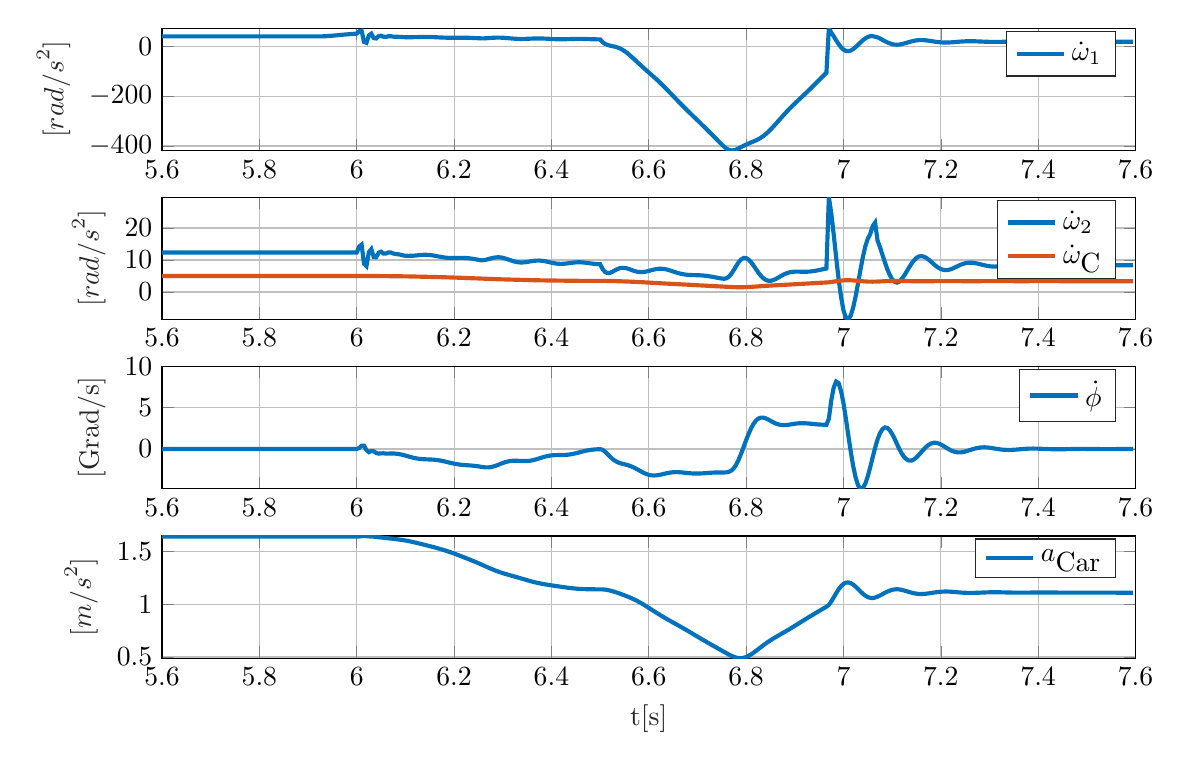
\begin{tikzpicture}

\begin{axis}[%
width=0.951\awidth,
height=0.194\aheight,
at={(0\awidth,0.806\aheight)},
scale only axis,
xmin=5.6,
xmax=7.6,
ymin=-417.664429354826,
ymax=72.7935981722241,
ylabel style={font=\color{white!15!black}},
ylabel={$\text{[rad/s}^\text{2}\text{]}$},
axis background/.style={fill=white},
xmajorgrids,
ymajorgrids,
legend style={legend cell align=left, align=left, draw=white!15!black}
]
\addplot [color=mycolor1, line width=1.5pt]
  table[row sep=crcr]{%
5.6	40.0360858533288\\
5.605	40.0361167967789\\
5.61	40.0361477133084\\
5.615	40.03617857401\\
5.62	40.0362094052232\\
5.625	40.0362401793584\\
5.63	40.0362709254895\\
5.635	40.0363016146811\\
5.64	40.0363322760286\\
5.645	40.0363628819075\\
5.65	40.0363934574151\\
5.655	40.0364239789503\\
5.66	40.0364544702514\\
5.665	40.0364849090093\\
5.67	40.0365153177049\\
5.675	40.0365456699484\\
5.68	40.0365759949108\\
5.685	40.0366062649342\\
5.69	40.0366365051229\\
5.695	40.0366666932176\\
5.7	40.0366968502741\\
5.705	40.0367725377863\\
5.71	40.0368389815492\\
5.715	40.0368886915464\\
5.72	40.0369193437496\\
5.725	40.0369377436488\\
5.73	40.0369543093394\\
5.735	40.036976489991\\
5.74	40.0370079553001\\
5.745	40.037047946015\\
5.75	40.0370926799768\\
5.755	40.0371385365792\\
5.76	40.0371821969765\\
5.765	40.0372226340834\\
5.77	40.0372601222993\\
5.775	40.0372961629141\\
5.78	40.0373325359807\\
5.785	40.0373708980486\\
5.79	40.0374122057864\\
5.795	40.0374570921719\\
5.8	40.0375053228833\\
5.805	40.0375568897206\\
5.81	40.0376112023581\\
5.815	40.0376683843832\\
5.82	40.0377282321123\\
5.825	40.0377914265074\\
5.83	40.0378583497105\\
5.835	40.0379302821816\\
5.84	40.0380080800697\\
5.845	40.0380935843313\\
5.85	40.038188058351\\
5.855	40.0382939944229\\
5.86	40.0384132169747\\
5.865	40.0385492177053\\
5.87	40.0387048051699\\
5.875	40.0388851210481\\
5.88	40.0390947114709\\
5.885	40.0393414483438\\
5.89	40.0396328332936\\
5.895	40.0399812167225\\
5.9	40.0419891033533\\
5.905	40.0459799738722\\
5.91	40.0496862898839\\
5.915	40.0536638093024\\
5.92	40.0592679568223\\
5.925	40.0685653831155\\
5.93	40.232866151909\\
5.935	40.6353960123335\\
5.94	41.2281492874086\\
5.945	41.9938412863546\\
5.95	42.8921612973889\\
5.955	43.6199502756565\\
5.96	44.5416408480299\\
5.965	45.5368451993716\\
5.97	46.4829310754561\\
5.975	47.3429215077385\\
5.98	48.1735020725965\\
5.985	48.9403023026508\\
5.99	49.5943567930395\\
5.995	50.4968568911064\\
6	51.2419538044049\\
6.005	60.3548929307732\\
6.01	62.6430650601239\\
6.015	18.1040280415948\\
6.02	14.3207707231346\\
6.025	44.09814406618\\
6.03	50.9879267682384\\
6.035	33.0794596566776\\
6.04	31.7251417269782\\
6.045	40.831678793929\\
6.05	42.9097522193509\\
6.055	38.5510416260345\\
6.06	38.0764487106552\\
6.065	40.4692599804846\\
6.07	40.6097100777422\\
6.075	38.938438145849\\
6.08	38.2665563727247\\
6.085	38.3469495379708\\
6.09	38.0198773761417\\
6.095	37.1887431247787\\
6.1	36.7279010615086\\
6.105	36.7323304976569\\
6.11	36.8232294671168\\
6.115	36.8416603227803\\
6.12	36.99004465219\\
6.125	37.2957784027737\\
6.13	37.5899689829282\\
6.135	37.7581516608303\\
6.14	37.8086532555277\\
6.145	37.7644903631247\\
6.15	37.5949025159786\\
6.155	37.2752736600746\\
6.16	36.8463522011887\\
6.165	36.3727497932095\\
6.17	35.8951811947805\\
6.175	35.443555279128\\
6.18	35.0613112954622\\
6.185	34.7826396534103\\
6.19	34.6134263180862\\
6.195	34.5409618504778\\
6.2	34.5459773316727\\
6.205	34.5988357823936\\
6.21	34.6595867212722\\
6.215	34.6880700183987\\
6.22	34.6524726989589\\
6.225	34.5308311427872\\
6.23	34.311798451696\\
6.235	33.998351279928\\
6.24	33.606822538989\\
6.245	33.1631580430518\\
6.25	32.6982601079238\\
6.255	32.2219357723467\\
6.26	32.0996475444554\\
6.265	32.475898056796\\
6.27	33.2433752879054\\
6.275	33.9623832864166\\
6.28	34.4852943926882\\
6.285	34.8975650980135\\
6.29	35.1264544107583\\
6.295	35.0319798230813\\
6.3	34.5763711157459\\
6.305	33.868350298903\\
6.31	33.024719619115\\
6.315	32.1722262435617\\
6.32	31.3671831407275\\
6.325	30.649947515688\\
6.33	30.1130854580637\\
6.335	29.8355419155659\\
6.34	29.8203075831594\\
6.345	30.0069257611115\\
6.35	30.3400355033562\\
6.355	30.7674791733117\\
6.36	31.2019947410255\\
6.365	31.5457554109754\\
6.37	31.7382124307706\\
6.375	31.7512524943599\\
6.38	31.572075906294\\
6.385	31.2107842812372\\
6.39	30.7135585698787\\
6.395	30.1470536770896\\
6.4	29.5794433203569\\
6.405	29.0745378604326\\
6.41	28.6893151528192\\
6.415	28.4630285978042\\
6.42	28.4091285415751\\
6.425	28.5141566900316\\
6.43	28.7465228196674\\
6.435	29.0590015339313\\
6.44	29.3939089648807\\
6.445	29.6936890451346\\
6.45	29.9102206775099\\
6.455	30.0101718597564\\
6.46	29.9783423290311\\
6.465	29.8196131926887\\
6.47	29.5579629080018\\
6.475	29.2316371226142\\
6.48	28.886690462414\\
6.485	28.5704180052266\\
6.49	28.3247489381814\\
6.495	28.1802495018807\\
6.5	28.1483029334591\\
6.505	17.5089482304227\\
6.51	10.1809140219622\\
6.515	5.72760532039593\\
6.52	2.97464603943853\\
6.525	0.988400792000554\\
6.53	-1.07678086005585\\
6.535	-3.81385455884178\\
6.54	-7.58445316186751\\
6.545	-12.5500704588089\\
6.55	-18.6503604950521\\
6.555	-25.7897830894559\\
6.56	-33.7760151701105\\
6.565	-42.3651991174332\\
6.57	-51.3176811741372\\
6.575	-60.422510448769\\
6.58	-69.521006628096\\
6.585	-78.5129843848206\\
6.59	-87.3583181207979\\
6.595	-96.0687468223414\\
6.6	-104.695106841566\\
6.605	-113.314657289094\\
6.61	-122.012267370453\\
6.615	-130.866702664061\\
6.62	-139.938773974937\\
6.625	-149.263745096454\\
6.63	-158.84823564019\\
6.635	-168.670571506867\\
6.64	-178.685968677258\\
6.645	-188.833451432688\\
6.65	-199.044484763492\\
6.655	-209.25152549\\
6.66	-219.395781753006\\
6.665	-229.432868692206\\
6.67	-239.336670853\\
6.675	-249.100094184509\\
6.68	-258.733668638872\\
6.685	-268.262170673927\\
6.69	-277.719992440156\\
6.695	-287.145771714393\\
6.7	-296.577226883947\\
6.705	-306.046656127542\\
6.71	-315.577579989834\\
6.715	-325.183051566266\\
6.72	-334.86557558142\\
6.725	-344.617360755384\\
6.73	-354.423074826757\\
6.735	-364.262551881089\\
6.74	-374.1138859636\\
6.745	-383.956266528427\\
6.75	-393.772425804402\\
6.755	-403.123231549089\\
6.76	-410.800481912981\\
6.765	-415.751950579352\\
6.77	-417.664429354826\\
6.775	-416.777017183334\\
6.78	-413.66710297143\\
6.785	-409.047512448918\\
6.79	-403.89660669851\\
6.795	-398.827568654643\\
6.8	-394.101514661699\\
6.805	-389.769483302399\\
6.81	-385.717587676769\\
6.815	-381.712185595134\\
6.82	-377.453348804041\\
6.825	-372.641609107635\\
6.83	-367.019324904296\\
6.835	-360.415252910424\\
6.84	-352.753570030764\\
6.845	-344.064978655367\\
6.85	-334.46553345199\\
6.855	-324.142091420937\\
6.86	-313.316897657585\\
6.865	-302.224534872852\\
6.87	-291.080195016906\\
6.875	-280.063803774385\\
6.88	-269.3028967871\\
6.885	-258.871403800544\\
6.89	-248.788136160247\\
6.895	-239.028698382228\\
6.9	-229.533284382815\\
6.905	-220.224737068881\\
6.91	-211.017188005327\\
6.915	-201.832744044196\\
6.92	-192.604832083184\\
6.925	-183.289008086685\\
6.93	-173.859179979382\\
6.935	-164.31208397128\\
6.94	-154.65826646365\\
6.945	-144.922696006766\\
6.95	-135.134027199155\\
6.955	-125.324677451451\\
6.96	-115.521426023419\\
6.965	-105.747386552451\\
6.97	72.7935981722241\\
6.975	55.4490355286459\\
6.98	40.3570579372353\\
6.985	24.2915230077808\\
6.99	9.11408473507417\\
6.995	-3.42662584658651\\
7	-13.0239592951734\\
7.005	-18.1872441341329\\
7.01	-19.3404925384138\\
7.015	-16.6889527009767\\
7.02	-11.0105208144504\\
7.025	-3.11424705176506\\
7.03	6.16826053337161\\
7.035	15.7868979706506\\
7.04	24.7814786364631\\
7.045	32.2320760275818\\
7.05	37.6297770458922\\
7.055	40.820264080916\\
7.06	41.1003733350938\\
7.065	38.6224766006298\\
7.07	36.3589383896286\\
7.075	31.6231175099223\\
7.08	26.3440358639844\\
7.085	21.0085465382988\\
7.09	16.1380069003845\\
7.095	12.0808811153089\\
7.1	8.98184173512114\\
7.105	7.12468202868895\\
7.11	6.570887215061\\
7.115	7.30649642987423\\
7.12	9.18947793882977\\
7.125	11.6844788889662\\
7.13	14.5015608044958\\
7.135	17.3660884339009\\
7.14	20.0452529890494\\
7.145	22.3027628559804\\
7.15	23.9988607268995\\
7.155	25.0182774083109\\
7.16	25.2800916870647\\
7.165	24.908770080892\\
7.17	24.047335752355\\
7.175	22.7926186412323\\
7.18	21.2994658683349\\
7.185	19.7453832864745\\
7.19	18.2866230370118\\
7.195	17.0638693081657\\
7.2	16.1596419223441\\
7.205	15.5866686300489\\
7.21	15.3541465873902\\
7.215	15.4927795470353\\
7.22	15.9493759444849\\
7.225	16.6247882334145\\
7.23	17.4305507466018\\
7.235	18.2694993052992\\
7.24	19.0598426359936\\
7.245	19.7227029140721\\
7.25	20.2105493199646\\
7.255	20.5094778051407\\
7.26	20.6258603028903\\
7.265	20.5588528465663\\
7.27	20.3456201130802\\
7.275	20.0134490611162\\
7.28	19.6074093382443\\
7.285	19.1760056778217\\
7.29	18.7655090159797\\
7.295	18.4053853975552\\
7.3	18.1262643595601\\
7.305	17.9456802877935\\
7.31	17.8738179413238\\
7.315	17.8971908869612\\
7.32	17.9976064794883\\
7.325	18.1709601378841\\
7.33	18.3802663883963\\
7.335	18.6004949816797\\
7.34	18.8130589256284\\
7.345	19.0027360176271\\
7.35	19.1527671815719\\
7.355	19.253572122846\\
7.36	19.300857531026\\
7.365	19.2962946978867\\
7.37	19.2481357620555\\
7.375	19.1629406436358\\
7.38	19.0547511583149\\
7.385	18.936991237992\\
7.39	18.822901784833\\
7.395	18.7226011257744\\
7.4	18.6415171781358\\
7.405	18.5862060385378\\
7.41	18.5567338275052\\
7.415	18.5545577016108\\
7.42	18.5772426668011\\
7.425	18.6180595837293\\
7.43	18.6713560392215\\
7.435	18.7304984658882\\
7.44	18.789212925478\\
7.445	18.8420475645623\\
7.45	18.8847491838125\\
7.455	18.9145409240724\\
7.46	18.9301745007437\\
7.465	18.9318667103923\\
7.47	18.9210288489207\\
7.475	18.9003926657898\\
7.48	18.8729044860584\\
7.485	18.8419085545726\\
7.49	18.8106628173421\\
7.495	18.7820526054459\\
7.5	18.7583641781635\\
7.505	18.7411401537771\\
7.51	18.7311399972217\\
7.515	18.7283477126188\\
7.52	18.7322717407003\\
7.525	18.7412421016728\\
7.53	18.7540427779343\\
7.535	18.7689298997312\\
7.54	18.7841732475995\\
7.545	18.7982669270957\\
7.55	18.8099898515226\\
7.555	18.8184878094577\\
7.56	18.8233100219747\\
7.565	18.8244024405326\\
7.57	18.8220401929987\\
7.575	18.8168807852129\\
7.58	18.809644979756\\
7.585	18.8012411545069\\
7.59	18.7925202258166\\
7.595	18.7842792731393\\
};
\addlegendentry{$\dot{\omega}_1$}

\end{axis}

\begin{axis}[%
width=0.951\awidth,
height=0.194\aheight,
at={(0\awidth,0.538\aheight)},
scale only axis,
xmin=5.6,
xmax=7.6,
ymin=-8.5245297968645,
ymax=29.6692322538102,
ylabel style={font=\color{white!15!black}},
ylabel={$\text{[rad/s}^\text{2}\text{]}$},
axis background/.style={fill=white},
xmajorgrids,
ymajorgrids,
legend style={legend cell align=left, align=left, draw=white!15!black}
]
\addplot [color=mycolor1, line width=1.5pt]
  table[row sep=crcr]{%
5.6	12.3444588354187\\
5.605	12.3444683767812\\
5.61	12.3444779079146\\
5.615	12.3444874224415\\
5.62	12.3444969272841\\
5.625	12.344506415765\\
5.63	12.3445158941058\\
5.635	12.3445253565951\\
5.64	12.3445348090881\\
5.645	12.3445442450884\\
5.65	12.3445536715308\\
5.655	12.3445630817832\\
5.66	12.3445724822413\\
5.665	12.344581866344\\
5.67	12.3445912408806\\
5.675	12.3446005995129\\
5.68	12.3446099481989\\
5.685	12.3446192807314\\
5.69	12.3446286041335\\
5.695	12.344637911011\\
5.7	12.3446472086207\\
5.705	12.3446543387417\\
5.71	12.3446628475904\\
5.715	12.3446726798875\\
5.72	12.3446831894189\\
5.725	12.3446936725295\\
5.73	12.3447036253528\\
5.735	12.3447128954458\\
5.74	12.3447216500326\\
5.745	12.34473016027\\
5.75	12.3447387057213\\
5.755	12.3447474622026\\
5.76	12.3447564499493\\
5.765	12.3447656387661\\
5.77	12.3447748977787\\
5.775	12.3447841475872\\
5.78	12.3447933013786\\
5.785	12.3448023457959\\
5.79	12.3448112709584\\
5.795	12.3448201235533\\
5.8	12.3448289077278\\
5.805	12.344837683605\\
5.81	12.3448464160001\\
5.815	12.3448551611837\\
5.82	12.3448638376203\\
5.825	12.344872506259\\
5.83	12.3448810540604\\
5.835	12.3448895637202\\
5.84	12.3448978957367\\
5.845	12.3449061665133\\
5.85	12.3449141936326\\
5.855	12.3449221385972\\
5.86	12.34492974358\\
5.865	12.3449372290052\\
5.87	12.3449442178817\\
5.875	12.3449510132168\\
5.88	12.3449570555795\\
5.885	12.3449627696727\\
5.89	12.3449673185223\\
5.895	12.3449713083546\\
5.9	12.3449980614541\\
5.905	12.3449940346036\\
5.91	12.3449950609765\\
5.915	12.3449998648175\\
5.92	12.3450028418229\\
5.925	12.3449956584336\\
5.93	12.3442033394522\\
5.935	12.3427046475599\\
5.94	12.3408099046856\\
5.945	12.3389536315308\\
5.95	12.3375953442664\\
5.955	12.3381881296618\\
5.96	12.3389396264756\\
5.965	12.3403753866623\\
5.97	12.3428967070286\\
5.975	12.34546044325\\
5.98	12.3483961178699\\
5.985	12.3494930806846\\
5.99	12.3487623763267\\
5.995	12.3523653839411\\
6	12.3500959337398\\
6.005	14.1829961148815\\
6.01	14.8048461703502\\
6.015	8.8613618363288\\
6.02	8.10737840965794\\
6.025	12.4661903562728\\
6.03	13.3903772475223\\
6.035	10.9127039291207\\
6.04	10.8590356972772\\
6.045	12.2497623763502\\
6.05	12.5975677383449\\
6.055	12.0364211581391\\
6.06	12.0111451566081\\
6.065	12.3511702828064\\
6.07	12.3334891947288\\
6.075	12.0317617925393\\
6.08	11.8575348822242\\
6.085	11.779912850584\\
6.09	11.643602697206\\
6.095	11.4480747450771\\
6.1	11.3277245654908\\
6.105	11.2982907081869\\
6.11	11.3058848713163\\
6.115	11.325951052886\\
6.12	11.3816045713693\\
6.125	11.4674283715794\\
6.13	11.5500470870547\\
6.135	11.6051833466754\\
6.14	11.626532219123\\
6.145	11.6130209008161\\
6.15	11.5587473257056\\
6.155	11.4618781672189\\
6.16	11.3329120727631\\
6.165	11.1877133529169\\
6.17	11.0396656468656\\
6.175	10.9006126319537\\
6.18	10.7830643711704\\
6.185	10.6961736130106\\
6.19	10.6424328604062\\
6.195	10.6190452740238\\
6.2	10.6198073249943\\
6.205	10.6352263857289\\
6.21	10.6533441844658\\
6.215	10.6621207474586\\
6.22	10.6515785970951\\
6.225	10.6147185386772\\
6.23	10.5480223057002\\
6.235	10.4523885315057\\
6.24	10.3326340068152\\
6.245	10.1965713985874\\
6.25	10.0536816108024\\
6.255	9.9394237897468\\
6.26	9.93999491671912\\
6.265	10.0599507177844\\
6.27	10.2692538141096\\
6.275	10.4827591320868\\
6.28	10.6589150579725\\
6.285	10.7911836712155\\
6.29	10.8554914525525\\
6.295	10.8249600591776\\
6.3	10.6909234959626\\
6.305	10.4769902517946\\
6.31	10.2250859099536\\
6.315	9.96125615002302\\
6.32	9.70793888091475\\
6.325	9.48715378686711\\
6.33	9.32407605769367\\
6.335	9.23660105894578\\
6.34	9.22663514882743\\
6.345	9.28142592350923\\
6.35	9.38399056148728\\
6.355	9.51446349703019\\
6.36	9.64636180980688\\
6.365	9.75258198283609\\
6.37	9.81391532233602\\
6.375	9.8196584328989\\
6.38	9.76571605443132\\
6.385	9.65646314613832\\
6.39	9.50543543033882\\
6.395	9.33206615277322\\
6.4	9.15741097341606\\
6.405	9.00169484425714\\
6.41	8.88237866115696\\
6.415	8.81127918955008\\
6.42	8.79282303441005\\
6.425	8.82351850884106\\
6.43	8.89369495117353\\
6.435	8.98880357013422\\
6.44	9.09133340474682\\
6.445	9.18372925804988\\
6.45	9.2510597551136\\
6.455	9.28286342275078\\
6.46	9.27433797177764\\
6.465	9.22684012213131\\
6.47	9.14751766899917\\
6.475	9.04793981137345\\
6.48	8.94219260609998\\
6.485	8.84481298940864\\
6.49	8.76871579272256\\
6.495	8.72338032138578\\
6.5	8.71424852556947\\
6.505	7.21850891292888\\
6.51	6.2697045073578\\
6.515	5.90558780000902\\
6.52	5.96550103331992\\
6.525	6.29169538754059\\
6.53	6.71957381954871\\
6.535	7.12119050471028\\
6.54	7.4109245185341\\
6.545	7.54706683078621\\
6.55	7.53211260974285\\
6.555	7.38445004645882\\
6.56	7.14452337599232\\
6.565	6.86416984393691\\
6.57	6.59417780503418\\
6.575	6.37773307889938\\
6.58	6.24409142288823\\
6.585	6.2069021622392\\
6.59	6.26389551672401\\
6.595	6.39930174327583\\
6.6	6.58755705307522\\
6.605	6.79711070465373\\
6.61	6.99582082947791\\
6.615	7.15489559346952\\
6.62	7.25228647627955\\
6.625	7.27474851280658\\
6.63	7.21857111135523\\
6.635	7.08929136446886\\
6.64	6.8999365506379\\
6.645	6.66879076312352\\
6.65	6.41666103563739\\
6.655	6.16419848306214\\
6.66	5.92948392771814\\
6.665	5.72626796174336\\
6.67	5.56277561143725\\
6.675	5.44145848760354\\
6.68	5.35940688170058\\
6.685	5.30936326546589\\
6.69	5.28111589360469\\
6.695	5.26311638848983\\
6.7	5.24403527138156\\
6.705	5.2141193059897\\
6.71	5.16620486221655\\
6.715	5.09623472995281\\
6.72	5.00328873551007\\
6.725	4.88952282903574\\
6.73	4.75935577352902\\
6.735	4.61867125015397\\
6.74	4.47390233151236\\
6.745	4.33119267979555\\
6.75	4.19567152622949\\
6.755	4.13235974844974\\
6.76	4.3077500482068\\
6.765	4.85220678592214\\
6.77	5.7654401157979\\
6.775	6.94149274281699\\
6.78	8.21678725450056\\
6.785	9.37608590325453\\
6.79	10.2074714488926\\
6.795	10.6181687403769\\
6.8	10.5818953127932\\
6.805	10.1325545340223\\
6.81	9.34417434728584\\
6.815	8.32636232975119\\
6.82	7.20387863460337\\
6.825	6.09866937432525\\
6.83	5.11637136931404\\
6.835	4.33496904161711\\
6.84	3.80073398238164\\
6.845	3.52632627127605\\
6.85	3.49566677148096\\
6.855	3.6691973141028\\
6.86	3.993262679292\\
6.865	4.40772274689698\\
6.87	4.85472110295905\\
6.875	5.28427445595798\\
6.88	5.65913871022212\\
6.885	5.95626441087461\\
6.89	6.1672128856485\\
6.895	6.29585985196354\\
6.9	6.35593587255835\\
6.905	6.3668858001447\\
6.91	6.35085115329957\\
6.915	6.3287777762871\\
6.92	6.31863537082199\\
6.925	6.33306440958313\\
6.93	6.37948731638926\\
6.935	6.45948011390556\\
6.94	6.57038233959429\\
6.945	6.7057614869027\\
6.95	6.85760819362486\\
6.955	7.01699843293409\\
6.96	7.17601999477392\\
6.965	7.32795805653541\\
6.97	29.6692322538102\\
6.975	24.5528073362093\\
6.98	17.9109918879772\\
6.985	10.8026592285232\\
6.99	4.08266603754282\\
6.995	-1.46569734414061\\
7	-5.71970214842713\\
7.005	-8.00838738765106\\
7.01	-8.5245297968645\\
7.015	-7.36400038753845\\
7.02	-4.85308975885573\\
7.025	-1.35835041081191\\
7.03	2.74639739664053\\
7.035	7.00672489733824\\
7.04	10.9884304861698\\
7.045	14.318142390197\\
7.05	16.6642355437953\\
7.055	18.1001931741162\\
7.06	20.5777464011639\\
7.065	21.6655312753091\\
7.07	16.1200928717917\\
7.075	14.0263373527714\\
7.08	11.6911712284732\\
7.085	9.33081959175706\\
7.09	7.17565299014541\\
7.095	5.37990180292763\\
7.1	4.00726697109303\\
7.105	3.18410446235339\\
7.11	2.93742952012008\\
7.115	3.24717871414532\\
7.12	4.12953322045405\\
7.125	5.19650380090934\\
7.13	6.43493815767988\\
7.135	7.70538620777506\\
7.14	8.89522055801172\\
7.145	9.89365592759805\\
7.15	10.6457826045248\\
7.155	11.0987866647356\\
7.16	11.2155369806887\\
7.165	11.0432573093481\\
7.17	10.6698416920908\\
7.175	10.1152719980673\\
7.18	9.45493281626887\\
7.185	8.76745842307128\\
7.19	8.12196137520959\\
7.195	7.58070041178416\\
7.2	7.18030646763236\\
7.205	6.92634427326902\\
7.21	6.82297433391113\\
7.215	6.88329728651979\\
7.22	7.08429820438414\\
7.225	7.38326319371708\\
7.23	7.73964247535696\\
7.235	8.1102117055857\\
7.24	8.46105848971592\\
7.245	8.75474021696073\\
7.25	8.97074542082964\\
7.255	9.10366193822529\\
7.26	9.15524363006398\\
7.265	9.12422733785797\\
7.27	9.03131148452167\\
7.275	8.88450663073263\\
7.28	8.70494989577674\\
7.285	8.51412910217641\\
7.29	8.33249134242897\\
7.295	8.17310124372352\\
7.3	8.04950902381688\\
7.305	7.96950362517646\\
7.31	7.93756549922909\\
7.315	7.95590906922962\\
7.32	7.98855629589252\\
7.325	8.07947308613029\\
7.33	8.16277155623493\\
7.335	8.25615847869267\\
7.34	8.35247779343399\\
7.345	8.4368578114063\\
7.35	8.50304376057466\\
7.355	8.54786997565134\\
7.36	8.56886856008668\\
7.365	8.56644253926652\\
7.37	8.54554356885183\\
7.375	8.50789666870196\\
7.38	8.46005645008654\\
7.385	8.4079684443991\\
7.39	8.35749194242908\\
7.395	8.31310315857672\\
7.4	8.27720029149714\\
7.405	8.25270007861582\\
7.41	8.23962418096289\\
7.415	8.23868010082106\\
7.42	8.24804540357718\\
7.425	8.26659650314559\\
7.43	8.29017168870996\\
7.435	8.31627656807541\\
7.44	8.34230142362048\\
7.445	8.36572118157437\\
7.45	8.38465221826755\\
7.455	8.39787297024895\\
7.46	8.40482685407051\\
7.465	8.40575098520958\\
7.47	8.4007673030078\\
7.475	8.39164006131796\\
7.48	8.37948687177686\\
7.485	8.36577748017407\\
7.49	8.35195354346843\\
7.495	8.33929192553387\\
7.5	8.32880484599673\\
7.505	8.32117577626195\\
7.51	8.31674157418547\\
7.515	8.31549629623805\\
7.52	8.3168413384642\\
7.525	8.3210289975118\\
7.53	8.32688865089403\\
7.535	8.33340254158065\\
7.54	8.34013727326146\\
7.545	8.34639568288821\\
7.55	8.35159227266558\\
7.555	8.35535993904296\\
7.56	8.35750327783217\\
7.565	8.35803028306054\\
7.57	8.35693809393933\\
7.575	8.35465589452906\\
7.58	8.35145661180104\\
7.585	8.34773904679787\\
7.59	8.34388033050072\\
7.595	8.34023293779182\\
};
\addlegendentry{$\dot{\omega}_2$}

\addplot [color=mycolor2, line width=1.5pt]
  table[row sep=crcr]{%
5.6	4.99774050300873\\
5.605	4.99774436418014\\
5.61	4.99774822005694\\
5.615	4.99775207056964\\
5.62	4.99775591580554\\
5.625	4.99775975569511\\
5.63	4.9977635903256\\
5.635	4.9977674196274\\
5.64	4.99777124368777\\
5.645	4.99777506243702\\
5.65	4.99777887596238\\
5.655	4.99778268419413\\
5.66	4.99778648721948\\
5.665	4.99779028496863\\
5.67	4.99779407752882\\
5.675	4.99779786483016\\
5.68	4.99780164695987\\
5.685	4.99780542384805\\
5.69	4.99780919558184\\
5.695	4.9978129620913\\
5.7	4.99781672346361\\
5.705	4.99782047993657\\
5.71	4.99782423033098\\
5.715	4.99782797505723\\
5.72	4.99783171435639\\
5.725	4.99783544844636\\
5.73	4.99783917772615\\
5.735	4.99784290235644\\
5.74	4.99784662251659\\
5.745	4.99785033807247\\
5.75	4.99785404893247\\
5.755	4.99785775479194\\
5.76	4.99786145550339\\
5.765	4.99786515081759\\
5.77	4.99786884071231\\
5.775	4.9978725250923\\
5.78	4.9978762040824\\
5.785	4.99787987770012\\
5.79	4.99788354613933\\
5.795	4.99788720944145\\
5.8	4.99789086778475\\
5.805	4.99789452116845\\
5.81	4.99789816970918\\
5.815	4.99790181333974\\
5.82	4.99790545210924\\
5.825	4.99790908589318\\
5.83	4.99791271469319\\
5.835	4.9979163383548\\
5.84	4.99791995686182\\
5.845	4.99792357005976\\
5.85	4.99792717793828\\
5.855	4.99793078036022\\
5.86	4.99793437732552\\
5.865	4.99793796870897\\
5.87	4.9979415544989\\
5.875	4.99794513455144\\
5.88	4.99794870879685\\
5.885	4.99795227702232\\
5.89	4.9979558390345\\
5.895	4.99795939448818\\
5.9	4.9979629300282\\
5.905	4.99796641874142\\
5.91	4.99796984923823\\
5.915	4.99797321741982\\
5.92	4.99797651898027\\
5.925	4.99797973502694\\
5.93	4.99798197887247\\
5.935	4.99798072592283\\
5.94	4.99797291168771\\
5.945	4.99795523614734\\
5.95	4.99792525100562\\
5.955	4.9978835142187\\
5.96	4.997832196419\\
5.965	4.99777367393949\\
5.97	4.99771180023199\\
5.975	4.99765176528473\\
5.98	4.99759883465355\\
5.985	4.9975584187722\\
5.99	4.99753210740251\\
5.995	4.9975190274204\\
6	4.99751741287588\\
6.005	4.99977639561069\\
6.01	5.00685362198219\\
6.015	5.01362702794096\\
6.02	5.0078761661919\\
6.025	5.00009133597546\\
6.03	4.99735133800362\\
6.035	4.99340664937259\\
6.04	4.9853283058232\\
6.045	4.97656793500899\\
6.05	4.96933390220487\\
6.055	4.96206481411845\\
6.06	4.95401823297508\\
6.065	4.94604207957095\\
6.07	4.93858006904639\\
6.075	4.93100859316804\\
6.08	4.92284131954094\\
6.085	4.91405376092315\\
6.09	4.90454356255745\\
6.095	4.89402624023015\\
6.1	4.88226174835254\\
6.105	4.86926884551148\\
6.11	4.85514208425963\\
6.115	4.83998298062429\\
6.12	4.82393308117649\\
6.125	4.80721671158169\\
6.13	4.79005012241079\\
6.135	4.77259471116174\\
6.14	4.75497005519955\\
6.145	4.73722220332332\\
6.15	4.71934014624177\\
6.155	4.70124149559751\\
6.16	4.68278408969681\\
6.165	4.66379749509135\\
6.17	4.64411113485623\\
6.175	4.62357301589524\\
6.18	4.60207088734504\\
6.185	4.57954748309131\\
6.19	4.55600932394165\\
6.195	4.53151877609335\\
6.2	4.50618398657522\\
6.205	4.48014129895679\\
6.21	4.45353528556462\\
6.215	4.42649673918224\\
6.22	4.39912435874352\\
6.225	4.37147326103143\\
6.23	4.34355090285911\\
6.235	4.31531284393891\\
6.24	4.28667585307695\\
6.245	4.2575302021046\\
6.25	4.22775663027701\\
6.255	4.1971884920865\\
6.26	4.16598596625721\\
6.265	4.13454475113008\\
6.27	4.10326955843197\\
6.275	4.07268563693346\\
6.28	4.04322161896892\\
6.285	4.01521588091507\\
6.29	3.98888323227646\\
6.295	3.96428471230602\\
6.3	3.94138340386602\\
6.305	3.91985603372114\\
6.31	3.89915729959542\\
6.315	3.87907156362929\\
6.32	3.85927037326069\\
6.325	3.83945211119474\\
6.33	3.81942183611667\\
6.335	3.79911085808592\\
6.34	3.77857935219684\\
6.345	3.75800402125431\\
6.35	3.73764621501273\\
6.355	3.71781039763425\\
6.36	3.6988074023068\\
6.365	3.68089947525348\\
6.37	3.66426377095242\\
6.375	3.64897675965497\\
6.38	3.63501228870667\\
6.385	3.6222375573656\\
6.39	3.61044418719348\\
6.395	3.59938139891513\\
6.4	3.58879353988988\\
6.405	3.57845603097584\\
6.41	3.56820456863425\\
6.415	3.5579583927722\\
6.42	3.54772391972407\\
6.425	3.537596544927\\
6.43	3.52773745177536\\
6.435	3.51834881859275\\
6.44	3.50964439598866\\
6.445	3.50181767096956\\
6.45	3.49501489513242\\
6.455	3.48931701720363\\
6.46	3.48473088828519\\
6.465	3.48119189849735\\
6.47	3.47857599213195\\
6.475	3.47672041967086\\
6.48	3.47544866761355\\
6.485	3.47459618355126\\
6.49	3.47403334611672\\
6.495	3.47368254546691\\
6.5	3.47352490849553\\
6.505	3.4717855642655\\
6.51	3.46597618545572\\
6.515	3.455468199411\\
6.52	3.44065623214126\\
6.525	3.42216574862908\\
6.53	3.40088928818346\\
6.535	3.37765574465768\\
6.54	3.35309785277773\\
6.545	3.32752986525616\\
6.55	3.30105122203202\\
6.555	3.27352621726011\\
6.56	3.24464582091836\\
6.565	3.21404128413653\\
6.57	3.18137356541213\\
6.575	3.14639869701559\\
6.58	3.10903354168806\\
6.585	3.06936924607156\\
6.59	3.02767053100919\\
6.595	2.98434330336112\\
6.6	2.93988802528569\\
6.605	2.89485018873535\\
6.61	2.84975489419771\\
6.615	2.80505917627652\\
6.62	2.76111128077592\\
6.625	2.71812797875858\\
6.63	2.67618857556491\\
6.635	2.63524162892292\\
6.64	2.59513078591181\\
6.645	2.55562590966536\\
6.65	2.51646033752059\\
6.655	2.47736690568093\\
6.66	2.4381101136566\\
6.665	2.39850955064197\\
6.67	2.35845567152161\\
6.675	2.3179132489012\\
6.68	2.27691617906193\\
6.685	2.23555451795476\\
6.69	2.19395663064224\\
6.695	2.15226848666149\\
6.7	2.1106337863747\\
6.705	2.06917663352773\\
6.71	2.02798862740612\\
6.715	1.98712224919342\\
6.72	1.94659047139259\\
6.725	1.9063674421966\\
6.73	1.86639871571268\\
6.735	1.82661125197817\\
6.74	1.78692489772278\\
6.745	1.74726287101909\\
6.75	1.70756081470081\\
6.755	1.66781445576045\\
6.76	1.62836814201842\\
6.765	1.59020766590382\\
6.77	1.55495562345558\\
6.775	1.5247767193652\\
6.78	1.50187791663144\\
6.785	1.48927646563348\\
6.79	1.48861980656842\\
6.795	1.4997176694874\\
6.8	1.52209813620012\\
6.805	1.55455287343866\\
6.81	1.59550027968291\\
6.815	1.64290701917578\\
6.82	1.69461720077496\\
6.825	1.74855808940493\\
6.83	1.80292484502514\\
6.835	1.85629915573517\\
6.84	1.90771494142812\\
6.845	1.95666391228893\\
6.85	2.00304958990867\\
6.855	2.04710931433761\\
6.86	2.08930931777422\\
6.865	2.13024004572175\\
6.87	2.17051383479636\\
6.875	2.21068444477467\\
6.88	2.25118834165616\\
6.885	2.2923130244665\\
6.89	2.33419118298582\\
6.895	2.37681378051216\\
6.9	2.42006090195833\\
6.905	2.4637379552978\\
6.91	2.50761694497598\\
6.915	2.55147171311129\\
6.92	2.59510801036282\\
6.925	2.63838248067999\\
6.93	2.68121232555464\\
6.935	2.72357515155301\\
6.94	2.76550118040468\\
6.945	2.80706046867573\\
6.95	2.84834727712483\\
6.955	2.88946445798955\\
6.96	2.93050972854744\\
6.965	2.97156486406472\\
6.97	3.02418384111007\\
6.975	3.12513824709721\\
6.98	3.24121673916359\\
6.985	3.36151475356012\\
6.99	3.47250920090417\\
6.995	3.56254235662688\\
7	3.63052296574211\\
7.005	3.66597951538666\\
7.01	3.67248522535902\\
7.015	3.65163099149097\\
7.02	3.60903811192541\\
7.025	3.55056578412548\\
7.03	3.48223588418768\\
7.035	3.41162069950523\\
7.04	3.34569911465573\\
7.045	3.29109974525714\\
7.05	3.25154258345566\\
7.055	3.2282311932586\\
7.06	3.22237772033957\\
7.065	3.23591309871437\\
7.07	3.26021099205686\\
7.075	3.29459875499386\\
7.08	3.33295938771922\\
7.085	3.37171698507129\\
7.09	3.40709731328294\\
7.095	3.43654716800074\\
7.1	3.45902637618643\\
7.105	3.47245138177278\\
7.11	3.47638121487997\\
7.115	3.47081179650203\\
7.12	3.45705317272751\\
7.125	3.43881678804104\\
7.13	3.41817844211513\\
7.135	3.39718944511834\\
7.14	3.37755903431342\\
7.145	3.36100124837129\\
7.15	3.34853497197067\\
7.155	3.34100085337289\\
7.16	3.33898396148756\\
7.165	3.34161398081509\\
7.17	3.34776343285465\\
7.175	3.35679927072179\\
7.18	3.36757387459566\\
7.185	3.37879167088034\\
7.19	3.3893149295533\\
7.195	3.3981188022177\\
7.2	3.40460043004209\\
7.205	3.40866975644353\\
7.21	3.41025846000335\\
7.215	3.40914506102021\\
7.22	3.40571140674779\\
7.225	3.40068172448694\\
7.23	3.3947045169197\\
7.235	3.38848431906217\\
7.24	3.38261577592996\\
7.245	3.37768063707495\\
7.25	3.37401832390186\\
7.255	3.37173403135153\\
7.26	3.37077837777156\\
7.265	3.37116601977747\\
7.27	3.37260949508052\\
7.275	3.37492316316901\\
7.28	3.37777539424334\\
7.285	3.38081196787804\\
7.29	3.38369646347143\\
7.295	3.38621375123364\\
7.3	3.38814086773256\\
7.305	3.38934961474969\\
7.31	3.38976675867709\\
7.315	3.38947636930948\\
7.32	3.38862802525639\\
7.325	3.38726847417007\\
7.33	3.38565397879967\\
7.335	3.38393954235875\\
7.34	3.3822805072778\\
7.345	3.3807916547748\\
7.35	3.37959118058613\\
7.355	3.37874943920619\\
7.36	3.37829763954948\\
7.365	3.37822645699167\\
7.37	3.37846803859457\\
7.375	3.37898157044269\\
7.38	3.37966273849398\\
7.385	3.38041357028267\\
7.39	3.38113751304896\\
7.395	3.3817609641463\\
7.4	3.38224451793701\\
7.405	3.38254008186518\\
7.41	3.38264744821368\\
7.415	3.38255581999517\\
7.42	3.38228379122669\\
7.425	3.38187827866218\\
7.43	3.38138242511405\\
7.435	3.38084388007251\\
7.44	3.38030834212185\\
7.445	3.37981565169834\\
7.45	3.37939678821506\\
7.455	3.37907198034638\\
7.46	3.37885032627345\\
7.465	3.37873007441848\\
7.47	3.37870158844862\\
7.475	3.37874421647922\\
7.48	3.37883668535739\\
7.485	3.3789546872587\\
7.49	3.37907447814287\\
7.495	3.37917503662714\\
7.5	3.37923970318919\\
7.505	3.37925723614578\\
7.51	3.37922210463508\\
7.515	3.37913442135041\\
7.52	3.3789984736617\\
7.525	3.37882442022357\\
7.53	3.37862291127029\\
7.535	3.378406368577\\
7.54	3.37818710007768\\
7.545	3.37797616993643\\
7.55	3.37778250686347\\
7.555	3.37761231753484\\
7.56	3.3774688855642\\
7.565	3.3773525656776\\
7.57	3.37726151516498\\
7.575	3.37719075384055\\
7.58	3.37713507353881\\
7.585	3.3770878863407\\
7.59	3.37704297512759\\
7.595	3.37699453811944\\
};
\addlegendentry{$\dot{\omega}_\textrm{C}$}

\end{axis}

\begin{axis}[%
width=0.951\awidth,
height=0.194\aheight,
at={(0\awidth,0.269\aheight)},
scale only axis,
xmin=5.6,
xmax=7.6,
ymin=-4.80602648435305,
ymax=10,
ylabel style={font=\color{white!15!black}},
ylabel={[Grad/s]},
axis background/.style={fill=white},
xmajorgrids,
ymajorgrids,
legend style={legend cell align=left, align=left, draw=white!15!black}
]
\addplot [color=mycolor1, line width=1.5pt]
  table[row sep=crcr]{%
5.6	0.00997805907192193\\
5.605	0.00998267479221076\\
5.61	0.00998729137638912\\
5.615	0.00999190837826337\\
5.62	0.00999652624036316\\
5.625	0.0100011445160877\\
5.63	0.0100057636491881\\
5.635	0.0100103831918421\\
5.64	0.010015003589022\\
5.645	0.010019624393313\\
5.65	0.0100242460480589\\
5.655	0.0100288681078802\\
5.66	0.0100334910161208\\
5.665	0.0100381143257729\\
5.67	0.0100427384826229\\
5.675	0.0100473630376276\\
5.68	0.0100519884369804\\
5.685	0.0100566142332664\\
5.69	0.0100612408698296\\
5.695	0.0100658679004762\\
5.7	0.0100704957701786\\
5.705	0.0100751127179071\\
5.71	0.0100797192578429\\
5.715	0.0100843199874905\\
5.72	0.0100889255633874\\
5.725	0.0100935453389089\\
5.73	0.0100981845918419\\
5.735	0.0101028413139079\\
5.74	0.0101075093504028\\
5.745	0.010112179144803\\
5.75	0.0101168426876067\\
5.755	0.0101214938045684\\
5.76	0.0101261307915216\\
5.765	0.0101307545567309\\
5.77	0.0101353691900334\\
5.775	0.0101399791093976\\
5.78	0.0101445894932754\\
5.785	0.0101492037670989\\
5.79	0.0101538248673595\\
5.795	0.01015845340106\\
5.8	0.0101630895408152\\
5.805	0.0101677316068852\\
5.81	0.010172378088074\\
5.815	0.0101770263585157\\
5.82	0.0101816745426498\\
5.825	0.0101863202336361\\
5.83	0.0101909621360476\\
5.835	0.010195598735024\\
5.84	0.0102002297134259\\
5.845	0.010204854578242\\
5.85	0.0102094738249263\\
5.855	0.0102140875845686\\
5.86	0.0102186965203526\\
5.865	0.0102233006216935\\
5.87	0.0102278998120544\\
5.875	0.0102324930769148\\
5.88	0.0102370787243212\\
5.885	0.010241654033958\\
5.89	0.0102462149957819\\
5.895	0.0102507566902635\\
5.9	0.0102548235150054\\
5.905	0.0102575104948252\\
5.91	0.0102589960314622\\
5.915	0.0102598782849655\\
5.92	0.0102603232316397\\
5.925	0.0102596770170226\\
5.93	0.0102131291422773\\
5.935	0.0100325123322707\\
5.94	0.00965775773767991\\
5.945	0.00906493094012458\\
5.95	0.00828745398048707\\
5.955	0.00748227209672486\\
5.96	0.00676419363011078\\
5.965	0.00618868173519425\\
5.97	0.0058453855776593\\
5.975	0.00582694315423883\\
5.98	0.00616175513564854\\
5.985	0.00683342306397022\\
5.99	0.00774021238387407\\
5.995	0.00868251904197424\\
6	0.0095480237296792\\
6.005	0.128652028333608\\
6.01	0.390789460740816\\
6.015	0.410460351487334\\
6.02	-0.130337403657198\\
6.025	-0.378292871956385\\
6.03	-0.24358129562627\\
6.035	-0.278418163535254\\
6.04	-0.471235405863656\\
6.045	-0.557623927445629\\
6.05	-0.522247813245464\\
6.055	-0.517093526430907\\
6.06	-0.549080745685414\\
6.065	-0.554013092087065\\
6.07	-0.533414068609328\\
6.075	-0.533727891561406\\
6.08	-0.561090281999428\\
6.085	-0.599244303506264\\
6.09	-0.646732966477252\\
6.095	-0.711142584574544\\
6.1	-0.791333173394636\\
6.105	-0.876226378107225\\
6.11	-0.958413158706575\\
6.115	-1.03489153792473\\
6.12	-1.10265830508462\\
6.125	-1.15722707414395\\
6.13	-1.19704126217929\\
6.135	-1.22369864541988\\
6.14	-1.24101289657318\\
6.145	-1.25284167187481\\
6.15	-1.26329351354253\\
6.155	-1.277365404789\\
6.16	-1.29939253318601\\
6.165	-1.33208294621614\\
6.17	-1.37638015517611\\
6.175	-1.43168594182696\\
6.18	-1.49595452133987\\
6.185	-1.56585107795317\\
6.19	-1.63729836552945\\
6.195	-1.70629305096146\\
6.2	-1.76938688490024\\
6.205	-1.82407941084081\\
6.21	-1.8691530597685\\
6.215	-1.90487347404034\\
6.22	-1.93282547973806\\
6.225	-1.95559561743318\\
6.23	-1.97638111820834\\
6.235	-1.99856640191276\\
6.24	-2.02515981495647\\
6.245	-2.05839973770648\\
6.25	-2.09947630222683\\
6.255	-2.14775892874594\\
6.26	-2.19256100661448\\
6.265	-2.22225510849218\\
6.27	-2.22369941662016\\
6.275	-2.19107229912621\\
6.28	-2.12713724226603\\
6.285	-2.03716478598189\\
6.29	-1.92799398970364\\
6.295	-1.80914700353327\\
6.3	-1.69359171298278\\
6.305	-1.59387425752341\\
6.31	-1.51317659557245\\
6.315	-1.45671618476708\\
6.32	-1.42463678689134\\
6.325	-1.41445552656215\\
6.33	-1.42084135079885\\
6.335	-1.43637589703596\\
6.34	-1.45166447675184\\
6.345	-1.45846456051942\\
6.35	-1.45012118934326\\
6.355	-1.42222683144932\\
6.36	-1.37327483310181\\
6.365	-1.30497940859928\\
6.37	-1.22188837842286\\
6.375	-1.13026807862893\\
6.38	-1.03722623859728\\
6.385	-0.94991268175271\\
6.39	-0.874343967209421\\
6.395	-0.814507883383882\\
6.4	-0.771973534672659\\
6.405	-0.74577715994564\\
6.41	-0.732736587086461\\
6.415	-0.727884591035896\\
6.42	-0.725314830769992\\
6.425	-0.719046314538945\\
6.43	-0.703952830896461\\
6.435	-0.676343373161175\\
6.44	-0.634508164320508\\
6.445	-0.578826830480031\\
6.45	-0.511659171469951\\
6.455	-0.436874265213457\\
6.46	-0.359249515101095\\
6.465	-0.283753345184468\\
6.47	-0.214827334476\\
6.475	-0.155765355209652\\
6.48	-0.108310176403463\\
6.485	-0.0724682179813087\\
6.49	-0.0465938383522673\\
6.495	-0.027697266955889\\
6.5	-0.0119499008815756\\
6.505	-0.0902987034024683\\
6.51	-0.307995535484971\\
6.515	-0.598538949346855\\
6.52	-0.900078125354767\\
6.525	-1.17406016371771\\
6.53	-1.39736188704198\\
6.535	-1.56508633501725\\
6.54	-1.68546267961621\\
6.545	-1.77346972301702\\
6.55	-1.84759398573192\\
6.555	-1.92329395472023\\
6.56	-2.0137653440416\\
6.565	-2.12634515635942\\
6.57	-2.26218835288642\\
6.575	-2.41705667328517\\
6.58	-2.58206436557465\\
6.585	-2.74600369300936\\
6.59	-2.89705071699352\\
6.595	-3.02457857843903\\
6.6	-3.12043432216184\\
6.605	-3.18006042661084\\
6.61	-3.20279716146241\\
6.615	-3.1916551533919\\
6.62	-3.15276566301097\\
6.625	-3.09438421290144\\
6.63	-3.02579675035619\\
6.635	-2.9561861448989\\
6.64	-2.89360466578828\\
6.645	-2.8442022114674\\
6.65	-2.81176133747476\\
6.655	-2.79757537924836\\
6.66	-2.80057520298706\\
6.665	-2.81779672408199\\
6.67	-2.84492850315334\\
6.675	-2.87702923029166\\
6.68	-2.90919227489502\\
6.685	-2.93712819745124\\
6.69	-2.95761036175546\\
6.695	-2.96872899271852\\
6.7	-2.96995397106463\\
6.705	-2.96203246717098\\
6.71	-2.94673367670739\\
6.715	-2.92649331414794\\
6.72	-2.90404140672994\\
6.725	-2.88204583337051\\
6.73	-2.86276227560866\\
6.735	-2.84782105295932\\
6.74	-2.83810602620616\\
6.745	-2.83376046043866\\
6.75	-2.83422770446011\\
6.755	-2.83595374512069\\
6.76	-2.82120337248369\\
6.765	-2.75361032270931\\
6.77	-2.59069056658719\\
6.775	-2.2956238459457\\
6.78	-1.85000507773462\\
6.785	-1.24518781768041\\
6.79	-0.518030132182188\\
6.795	0.272269920479622\\
6.8	1.0703228125395\\
6.805	1.82374167070824\\
6.81	2.48762183031218\\
6.815	3.02883362293378\\
6.82	3.42877340078312\\
6.825	3.6838774711281\\
6.83	3.80401432774147\\
6.835	3.80977934684604\\
6.84	3.72864890589217\\
6.845	3.5911476803001\\
6.85	3.42706161113956\\
6.855	3.26246158518006\\
6.86	3.11758183398102\\
6.865	3.00571550050506\\
6.87	2.93316010769444\\
6.875	2.89987152122345\\
6.88	2.90086133922803\\
6.885	2.92776556419871\\
6.89	2.97064817831644\\
6.895	3.01951228712604\\
6.9	3.06562771044299\\
6.905	3.10235198499964\\
6.91	3.12559544755572\\
6.915	3.13382578440813\\
6.92	3.12778528759871\\
6.925	3.10994721693386\\
6.93	3.08388407666877\\
6.935	3.05358966592844\\
6.94	3.02291155726865\\
6.945	2.99506829700147\\
6.95	2.97238817546672\\
6.955	2.95615132876706\\
6.96	2.94665856049367\\
6.965	2.94334029760872\\
6.97	3.65966169218054\\
6.975	5.91602235846493\\
6.98	7.45601279516172\\
6.985	8.1766653888356\\
6.99	7.99262715800486\\
6.995	7.02831067827909\\
7	5.56892644150393\\
7.005	3.68087929943239\\
7.01	1.64944206048156\\
7.015	-0.323736566444773\\
7.02	-2.06660167516203\\
7.025	-3.45454114175947\\
7.03	-4.38424744269714\\
7.035	-4.80602648435305\\
7.04	-4.72901855293459\\
7.045	-4.1807770292758\\
7.05	-3.29707177011146\\
7.055	-2.20244827767777\\
7.06	-1.00788256808443\\
7.065	0.136905662928806\\
7.07	1.1594394565715\\
7.075	1.91636484335472\\
7.08	2.40085384184045\\
7.085	2.62094341618513\\
7.09	2.56130518596717\\
7.095	2.27766592830057\\
7.1	1.8313535039068\\
7.105	1.2536572572937\\
7.11	0.608714888530917\\
7.115	-0.028280107514011\\
7.12	-0.570325744688409\\
7.125	-0.989063893534218\\
7.13	-1.27136185882929\\
7.135	-1.39987098533529\\
7.14	-1.39117150800851\\
7.145	-1.25214369316502\\
7.15	-1.0134270327806\\
7.155	-0.704489928202159\\
7.16	-0.363320606433029\\
7.165	-0.0312879688891392\\
7.17	0.267912584206545\\
7.175	0.508798943879421\\
7.18	0.672646086737277\\
7.185	0.753907743182969\\
7.19	0.754306231050538\\
7.195	0.681488813973599\\
7.2	0.554070212480165\\
7.205	0.392020322316774\\
7.21	0.211152343277127\\
7.215	0.0281531588438702\\
7.22	-0.136274258916251\\
7.225	-0.268813501797483\\
7.23	-0.359806098206851\\
7.235	-0.405020686703819\\
7.24	-0.407839504719784\\
7.245	-0.370401117383495\\
7.25	-0.30318470778919\\
7.255	-0.217592495341654\\
7.26	-0.12303831860145\\
7.265	-0.0288421735166104\\
7.27	0.0574379439456937\\
7.275	0.128322397296035\\
7.28	0.178784371599282\\
7.285	0.205599985284508\\
7.29	0.209818539781227\\
7.295	0.195019087683528\\
7.3	0.163459878202701\\
7.305	0.120125202377476\\
7.31	0.0706426830377966\\
7.315	0.0209030431607193\\
7.32	-0.0252609600200841\\
7.325	-0.0621928821277183\\
7.33	-0.0886252595980717\\
7.335	-0.104180329638013\\
7.34	-0.1080517941387\\
7.345	-0.101959288201336\\
7.35	-0.0869221452977494\\
7.355	-0.0654045338627601\\
7.36	-0.0401768399559746\\
7.365	-0.0141359620710127\\
7.37	0.0103801753781521\\
7.375	0.0309083814953469\\
7.38	0.0459365962108611\\
7.385	0.0550229211539843\\
7.39	0.0573494936034331\\
7.395	0.0542107795676441\\
7.4	0.0467130308254802\\
7.405	0.0357716158597016\\
7.41	0.0228819952193415\\
7.415	0.00933787490418154\\
7.42	-0.00339469486594426\\
7.425	-0.0142384444224819\\
7.43	-0.0224149696039793\\
7.435	-0.0274930538169023\\
7.44	-0.0293788178787526\\
7.445	-0.0282910576953981\\
7.45	-0.0246942410135635\\
7.455	-0.0192330255878362\\
7.46	-0.0126432929453119\\
7.465	-0.00567768447890844\\
7.47	0.000961655712830593\\
7.475	0.00670337863059841\\
7.48	0.0111249706591998\\
7.485	0.0139778731674726\\
7.49	0.0151882974712281\\
7.495	0.0148465047908978\\
7.5	0.0131739428276011\\
7.505	0.0104906668410007\\
7.51	0.00716982892443167\\
7.515	0.00359924438446519\\
7.52	0.000145484886643072\\
7.525	-0.00288693269238004\\
7.53	-0.00526872071752363\\
7.535	-0.00685845950862028\\
7.54	-0.00760513119031848\\
7.545	-0.00754337239718282\\
7.55	-0.00677766689494312\\
7.555	-0.00546622594760716\\
7.56	-0.00379773369506227\\
7.565	-0.001971558367984\\
7.57	-0.000178318917975055\\
7.575	0.00141947233693703\\
7.58	0.00269529571331311\\
7.585	0.00357475570277926\\
7.59	0.00402282465449793\\
7.595	0.00405106517059632\\
};
\addlegendentry{$\dot{\phi}$}

\end{axis}

\begin{axis}[%
width=0.951\awidth,
height=0.194\aheight,
at={(0\awidth,0\aheight)},
scale only axis,
xmin=5.6,
xmax=7.6,
xlabel style={font=\color{white!15!black}},
xlabel={t[s]},
ymin=0.48930933041904,
ymax=1.64797920408419,
ylabel style={font=\color{white!15!black}},
ylabel={$\text{[m/s}^\text{2}\text{]}$},
axis background/.style={fill=white},
xmajorgrids,
ymajorgrids,
legend style={legend cell align=left, align=left, draw=white!15!black}
]
\addplot [color=mycolor1, line width=1.5pt]
  table[row sep=crcr]{%
5.6	1.64275730333897\\
5.605	1.64275857250601\\
5.61	1.64275983993272\\
5.615	1.64276110559624\\
5.62	1.64276236952528\\
5.625	1.64276363169698\\
5.63	1.64276489214003\\
5.635	1.64276615083153\\
5.64	1.64276740780017\\
5.645	1.64276866302305\\
5.65	1.64276991652883\\
5.655	1.64277116829461\\
5.66	1.64277241834904\\
5.665	1.64277366666919\\
5.67	1.64277491328372\\
5.675	1.64277615816967\\
5.68	1.64277740135571\\
5.685	1.64277864281885\\
5.69	1.64277988258775\\
5.695	1.64278112063941\\
5.7	1.64278235700249\\
5.705	1.64278359175515\\
5.71	1.64278482450979\\
5.715	1.64278605540131\\
5.72	1.64278728450894\\
5.725	1.64278851190432\\
5.73	1.64278973771859\\
5.735	1.64279096200456\\
5.74	1.6427921848212\\
5.745	1.64279340612442\\
5.75	1.6427946258841\\
5.755	1.64279584400011\\
5.76	1.64279706042397\\
5.765	1.64279827507374\\
5.77	1.64279948794214\\
5.775	1.64280069899784\\
5.78	1.64280190828189\\
5.785	1.64280311580003\\
5.79	1.642804321616\\
5.795	1.6428055257434\\
5.8	1.64280672824085\\
5.805	1.64280792910807\\
5.81	1.64280912838341\\
5.815	1.64281032604477\\
5.82	1.64281152210831\\
5.825	1.64281271653309\\
5.83	1.64281390931965\\
5.835	1.64281510041722\\
5.84	1.64281628982048\\
5.845	1.64281747747864\\
5.85	1.64281866338831\\
5.855	1.64281984750441\\
5.86	1.6428210298269\\
5.865	1.64282221031464\\
5.87	1.64282338896379\\
5.875	1.64282456572706\\
5.88	1.64282574058152\\
5.885	1.64282691345724\\
5.89	1.64282808429064\\
5.895	1.64282925296826\\
5.9	1.64283041510027\\
5.905	1.6428315618403\\
5.91	1.64283268944461\\
5.915	1.6428337965659\\
5.92	1.64283488178882\\
5.925	1.64283593890336\\
5.93	1.64283667645538\\
5.935	1.64283626461083\\
5.94	1.64283369607175\\
5.945	1.64282788612163\\
5.95	1.64281803000555\\
5.955	1.64280431112369\\
5.96	1.64278744296293\\
5.965	1.64276820662391\\
5.97	1.64274786873626\\
5.975	1.64272813524909\\
5.98	1.64271073695062\\
5.985	1.64269745225042\\
5.99	1.6426888037032\\
5.995	1.64268450431309\\
6	1.6426839736123\\
6.005	1.64342650123723\\
6.01	1.64575278554555\\
6.015	1.64797920408419\\
6.02	1.64608889582728\\
6.025	1.64353002213513\\
6.03	1.64262938480179\\
6.035	1.64133276564877\\
6.04	1.63867741412409\\
6.045	1.63579788023746\\
6.05	1.63342005365474\\
6.055	1.63103070440073\\
6.06	1.62838579317891\\
6.065	1.62576403155497\\
6.07	1.62331126869555\\
6.075	1.62082252457433\\
6.08	1.61813794173311\\
6.085	1.61524947121544\\
6.09	1.61212346901263\\
6.095	1.60866642516365\\
6.1	1.60479943668348\\
6.105	1.60052866951962\\
6.11	1.59588520309614\\
6.115	1.5909024057312\\
6.12	1.58562680378271\\
6.125	1.5801321330969\\
6.13	1.57448947523643\\
6.135	1.56875188155886\\
6.14	1.56295865714409\\
6.145	1.55712493823238\\
6.15	1.55124710606967\\
6.155	1.5452980796029\\
6.16	1.53923113028334\\
6.165	1.53299023663653\\
6.17	1.52651933002724\\
6.175	1.51976845032477\\
6.18	1.51270070067031\\
6.185	1.50529725769211\\
6.19	1.49756026477962\\
6.195	1.48951022170189\\
6.2	1.48118267638727\\
6.205	1.4726224449671\\
6.21	1.46387704836509\\
6.215	1.4549894781692\\
6.22	1.445992176719\\
6.225	1.43690326090103\\
6.23	1.42772518176979\\
6.235	1.41844333180272\\
6.24	1.40903035290639\\
6.245	1.39945017743178\\
6.25	1.38966360437205\\
6.255	1.37961585734883\\
6.26	1.36935958710874\\
6.265	1.35902485969646\\
6.27	1.34874470385659\\
6.275	1.33869176886003\\
6.28	1.32900694615508\\
6.285	1.31980146005678\\
6.29	1.31114591844927\\
6.295	1.30306038493499\\
6.3	1.29553272485076\\
6.305	1.28845667828414\\
6.31	1.28165300437702\\
6.315	1.27505082296495\\
6.32	1.26854217169079\\
6.325	1.26202790894971\\
6.33	1.25544395753155\\
6.335	1.24876773905284\\
6.34	1.2420190330671\\
6.345	1.23525592178629\\
6.35	1.22856431087468\\
6.355	1.22204427770238\\
6.36	1.21579799313824\\
6.365	1.20991165751582\\
6.37	1.20444350151206\\
6.375	1.19941866089859\\
6.38	1.19482853929788\\
6.385	1.19062948510607\\
6.39	1.1867530043305\\
6.395	1.1831166658234\\
6.4	1.1796364365618\\
6.405	1.17623849738176\\
6.41	1.17286884171008\\
6.415	1.16950092370422\\
6.42	1.1661368524133\\
6.425	1.1628079843175\\
6.43	1.15956730039856\\
6.435	1.15648125667144\\
6.44	1.15362011296147\\
6.445	1.15104746844769\\
6.45	1.14881139603003\\
6.455	1.14693850355483\\
6.46	1.14543104297934\\
6.465	1.14426777703608\\
6.47	1.14340792861377\\
6.475	1.14279800194581\\
6.48	1.14237997704457\\
6.485	1.1420997655333\\
6.49	1.14191476086857\\
6.495	1.14179945269497\\
6.5	1.14174763742248\\
6.505	1.14117591497407\\
6.51	1.13926637215929\\
6.515	1.1358123971464\\
6.52	1.13094370350483\\
6.525	1.12486588157438\\
6.53	1.1178723090259\\
6.535	1.11023544326898\\
6.54	1.10216326420804\\
6.545	1.0937590667097\\
6.55	1.08505553668192\\
6.555	1.0760080676134\\
6.56	1.06651508133587\\
6.565	1.05645537009568\\
6.57	1.04571749095097\\
6.575	1.03422125170902\\
6.58	1.02193932515287\\
6.585	1.00890167118372\\
6.59	0.99519530354272\\
6.595	0.9809536438148\\
6.6	0.966341193911406\\
6.605	0.951537257037311\\
6.61	0.936714433722787\\
6.615	0.922022951242092\\
6.62	0.907577277991046\\
6.625	0.893448666617946\\
6.63	0.879663184788185\\
6.635	0.866203923426963\\
6.64	0.853019489329213\\
6.645	0.840034236507003\\
6.65	0.827160512943018\\
6.655	0.81431050189732\\
6.66	0.801406794358925\\
6.665	0.788390089296016\\
6.67	0.775224379229153\\
6.675	0.761898084913826\\
6.68	0.748422348057657\\
6.685	0.734826770051729\\
6.69	0.721153544492104\\
6.695	0.707450651565631\\
6.7	0.693765325581363\\
6.705	0.680138359440564\\
6.71	0.666599861828393\\
6.715	0.653167083309876\\
6.72	0.639844287946744\\
6.725	0.626622978250022\\
6.73	0.613485257854757\\
6.735	0.600407118525223\\
6.74	0.587362213881478\\
6.745	0.574325305703976\\
6.75	0.561275239792157\\
6.755	0.548210611608459\\
6.76	0.535244608281456\\
6.765	0.522701259782585\\
6.77	0.51111391342985\\
6.775	0.501194107655343\\
6.78	0.493667271196755\\
6.785	0.489525174253725\\
6.79	0.48930933041904\\
6.795	0.492957197960507\\
6.8	0.500313657368978\\
6.805	0.510981529499286\\
6.81	0.524440941931771\\
6.815	0.540023537203078\\
6.82	0.55702067389473\\
6.825	0.574751043987402\\
6.83	0.592621396559763\\
6.835	0.610165532490151\\
6.84	0.627065901247424\\
6.845	0.643155427969371\\
6.85	0.65840240020298\\
6.855	0.672884831622771\\
6.86	0.686755972752387\\
6.865	0.700209903028738\\
6.87	0.713447897497563\\
6.875	0.726651976997433\\
6.88	0.739965607902381\\
6.885	0.753483291142138\\
6.89	0.767248641847441\\
6.895	0.781258689654346\\
6.9	0.795474018473703\\
6.905	0.809830665906386\\
6.91	0.824253689813604\\
6.915	0.838668752099683\\
6.92	0.85301200300626\\
6.925	0.867236321399513\\
6.93	0.881314491409809\\
6.935	0.895239152315473\\
6.94	0.909020237999018\\
6.945	0.922680776053714\\
6.95	0.93625174999093\\
6.955	0.949766967341165\\
6.96	0.963258547773545\\
6.965	0.976753370818073\\
6.97	0.99404922857288\\
6.975	1.02723294182085\\
6.98	1.06538794216307\\
6.985	1.10492989949521\\
6.99	1.1414137743372\\
6.995	1.17100767262326\\
7	1.19335289883943\\
7.005	1.20500746670759\\
7.01	1.20714589357551\\
7.015	1.20029110690308\\
7.02	1.18629082738988\\
7.025	1.16707097324204\\
7.03	1.14461093513249\\
7.035	1.12139972392737\\
7.04	1.09973129898734\\
7.045	1.08178448626602\\
7.05	1.06878204718187\\
7.055	1.0611195932241\\
7.06	1.05919555667562\\
7.065	1.06364463554741\\
7.07	1.07163135308909\\
7.075	1.08293461076648\\
7.08	1.09554375074331\\
7.085	1.10828337299293\\
7.09	1.1199128868761\\
7.095	1.12959305412184\\
7.1	1.13698196985248\\
7.105	1.14139476918871\\
7.11	1.14268650533105\\
7.115	1.14085583751022\\
7.12	1.13633337787553\\
7.125	1.13033907822909\\
7.13	1.12355525392324\\
7.135	1.1166561706104\\
7.14	1.11020365457882\\
7.145	1.10476111033964\\
7.15	1.10066344528676\\
7.155	1.09818698050367\\
7.16	1.09752402814096\\
7.165	1.09838851549392\\
7.17	1.10040984037932\\
7.175	1.10337992028625\\
7.18	1.10692153257959\\
7.185	1.11060882221837\\
7.19	1.11406781734417\\
7.195	1.11696165028896\\
7.2	1.11909216135484\\
7.205	1.12042974894299\\
7.21	1.1209519558031\\
7.215	1.12058598155734\\
7.22	1.119457339398\\
7.225	1.11780408283886\\
7.23	1.11583937471151\\
7.235	1.11379479567574\\
7.24	1.11186580554818\\
7.245	1.11024362540654\\
7.25	1.10903982306654\\
7.255	1.10828897610525\\
7.26	1.10797485277351\\
7.265	1.10810227070085\\
7.27	1.10857674103297\\
7.275	1.10933724373365\\
7.28	1.11027477208779\\
7.285	1.11127289384151\\
7.29	1.11222102754306\\
7.295	1.1130484600305\\
7.3	1.11368190322369\\
7.305	1.11407921836822\\
7.31	1.11421633357716\\
7.315	1.11412088259203\\
7.32	1.11384203190178\\
7.325	1.1133951474597\\
7.33	1.11286446283145\\
7.335	1.11230092757332\\
7.34	1.11175560274221\\
7.345	1.11126621692448\\
7.35	1.11087162105866\\
7.355	1.11059494066707\\
7.36	1.11044643411991\\
7.365	1.11042303641316\\
7.37	1.11050244428603\\
7.375	1.11067124220451\\
7.38	1.11089514214297\\
7.385	1.11114194055191\\
7.39	1.11137990053919\\
7.395	1.11158482891489\\
7.4	1.11174377304589\\
7.405	1.11184092490909\\
7.41	1.11187621622784\\
7.415	1.11184609803241\\
7.42	1.11175668217621\\
7.425	1.11162339019626\\
7.43	1.11146040313499\\
7.435	1.11128338337984\\
7.44	1.11110735205545\\
7.445	1.11094540471324\\
7.45	1.11080772428629\\
7.455	1.11070095993986\\
7.46	1.11062810224608\\
7.465	1.11058857546135\\
7.47	1.11057921212306\\
7.475	1.11059322395672\\
7.48	1.11062361847697\\
7.485	1.11066240570193\\
7.49	1.11070178096556\\
7.495	1.11073483453934\\
7.5	1.11075609043829\\
7.505	1.11076185352112\\
7.51	1.11075030579355\\
7.515	1.11072148429788\\
7.52	1.1106767982926\\
7.525	1.11061958692749\\
7.53	1.11055335093454\\
7.535	1.11048217335126\\
7.54	1.11041009979553\\
7.545	1.1103407670581\\
7.55	1.11027711000602\\
7.555	1.1102211687737\\
7.56	1.11017402268495\\
7.565	1.11013578833823\\
7.57	1.11010586003473\\
7.575	1.11008260078739\\
7.58	1.11006429867221\\
7.585	1.11004878824019\\
7.59	1.11003402592444\\
7.595	1.11001810467986\\
};
\addlegendentry{$a_\textrm{Car}$}

\end{axis}
\end{tikzpicture}%
\caption{Zeitlicher Verlauf der Beschleunigungen und Verdrehungsgeschwindigkeit der Seitenwellen  beim Gangwechsel}
\label{fig:Gang23_Besch}
\end{figure}

\begin{figure}[h]
\centering
\newlength\bheight 
\setlength\bheight{16cm}
\newlength\bwidth 
\setlength\bwidth{13cm}
% This file was created by matlab2tikz.
%
%The latest updates can be retrieved from
%  http://www.mathworks.com/matlabcentral/fileexchange/22022-matlab2tikz-matlab2tikz
%where you can also make suggestions and rate matlab2tikz.
%
\definecolor{mycolor1}{rgb}{0.00000,0.44700,0.74100}%
\definecolor{mycolor2}{rgb}{0.85000,0.32500,0.09800}%
%
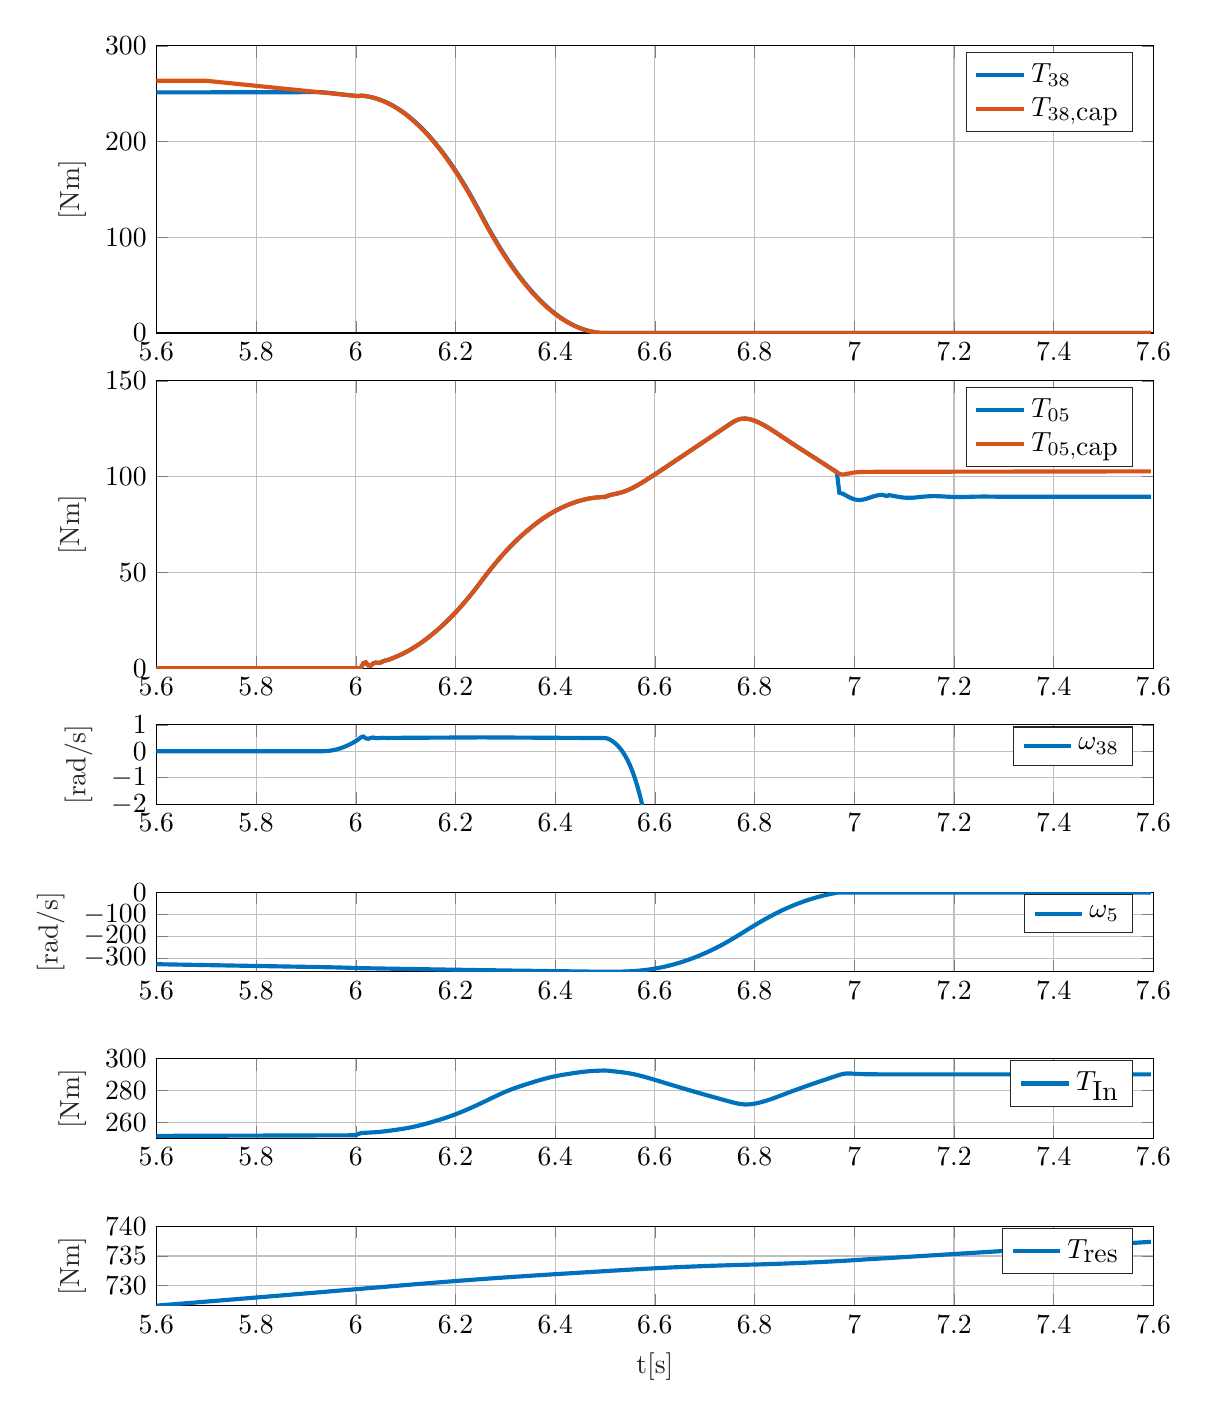
\begin{tikzpicture}

\begin{axis}[%
width=0.974\bwidth,
height=0.228\bheight,
at={(0\bwidth,0.772\bheight)},
scale only axis,
xmin=5.6,
xmax=7.6,
ymin=0,
ymax=300,
ylabel style={font=\color{white!15!black}},
ylabel={[Nm]},
axis background/.style={fill=white},
xmajorgrids,
ymajorgrids,
legend style={legend cell align=left, align=left, draw=white!15!black}
]
\addplot [color=mycolor1, line width=1.5pt]
  table[row sep=crcr]{%
5.6	251.324196937571\\
5.605	251.328551978443\\
5.61	251.33290902851\\
5.615	251.337268082622\\
5.62	251.341629146506\\
5.625	251.345992215012\\
5.63	251.350357293865\\
5.635	251.354724377912\\
5.64	251.359093472863\\
5.645	251.363464573576\\
5.65	251.367837685763\\
5.655	251.372212804266\\
5.66	251.376589934811\\
5.665	251.38096907223\\
5.67	251.385350222247\\
5.675	251.389733379721\\
5.68	251.394118550343\\
5.685	251.398505728966\\
5.69	251.402894921311\\
5.695	251.407286122193\\
5.7	251.411679337349\\
5.705	251.416062910737\\
5.71	251.420448640354\\
5.715	251.424839501019\\
5.72	251.429237905621\\
5.725	251.433642936822\\
5.73	251.43805188699\\
5.735	251.44246224286\\
5.74	251.446872226069\\
5.745	251.451281418915\\
5.75	251.455690607773\\
5.755	251.460100739669\\
5.76	251.464513084839\\
5.765	251.46892813986\\
5.77	251.473346189598\\
5.775	251.477766875941\\
5.78	251.482189783152\\
5.785	251.486614294736\\
5.79	251.491040084976\\
5.795	251.495466751604\\
5.8	251.499894367646\\
5.805	251.504322740688\\
5.81	251.508752176545\\
5.815	251.513182465594\\
5.82	251.517613896696\\
5.825	251.522046067573\\
5.83	251.526479142127\\
5.835	251.530912463331\\
5.84	251.535346091906\\
5.845	251.539779094508\\
5.85	251.54421148146\\
5.855	251.54864197792\\
5.86	251.553070556517\\
5.865	251.557495442153\\
5.87	251.561916518511\\
5.875	251.566331224249\\
5.88	251.570739232882\\
5.885	251.575136730134\\
5.89	251.579522967702\\
5.895	251.583892124382\\
5.9	251.587597690766\\
5.905	251.590655911881\\
5.91	251.593827451309\\
5.915	251.596912102685\\
5.92	251.599424356877\\
5.925	251.600626352389\\
5.93	251.546773355117\\
5.935	251.407267763264\\
5.94	251.200277998441\\
5.945	250.932248443384\\
5.95	250.617986110781\\
5.955	250.366732540807\\
5.96	250.046928719455\\
5.965	249.701923339615\\
5.97	249.375011920781\\
5.975	249.081076198104\\
5.98	248.796192446428\\
5.985	248.536640639005\\
5.99	248.320516814436\\
5.995	247.994706011143\\
6	247.738789781753\\
6.005	247.472310914202\\
6.01	247.861288594238\\
6.015	247.814492592787\\
6.02	247.493158181057\\
6.025	247.069550794376\\
6.03	246.546149568244\\
6.035	245.923855168622\\
6.04	245.202094174683\\
6.045	244.38086110607\\
6.05	243.460147884481\\
6.055	242.441088965125\\
6.06	241.322198550205\\
6.065	240.104022659404\\
6.07	238.786565847269\\
6.075	237.369828186045\\
6.08	235.853809679764\\
6.085	234.238510328337\\
6.09	232.523930131708\\
6.095	230.710069089877\\
6.1	228.796927202845\\
6.105	226.784504470611\\
6.11	224.672800893176\\
6.115	222.46181647054\\
6.12	220.151551202701\\
6.125	217.742005089662\\
6.13	215.233178131421\\
6.135	212.625070327978\\
6.14	209.917681679333\\
6.145	207.111012185487\\
6.15	204.20506184644\\
6.155	201.199830662191\\
6.16	198.095318632741\\
6.165	194.891525758089\\
6.17	191.588452038236\\
6.175	188.186097473181\\
6.18	184.684462062925\\
6.185	181.083545807466\\
6.19	177.383348706807\\
6.195	173.583870760946\\
6.2	169.685111969884\\
6.205	165.68707233362\\
6.21	161.589751852154\\
6.215	157.393150525487\\
6.22	153.097268353619\\
6.225	148.702105336548\\
6.23	144.207661474276\\
6.235	139.613936766803\\
6.24	134.920931214129\\
6.245	130.128644816253\\
6.25	125.237077573175\\
6.255	120.313741733389\\
6.26	115.475705221927\\
6.265	110.734669253283\\
6.27	106.095236064131\\
6.275	101.555121242504\\
6.28	97.1142889599688\\
6.285	92.772737596481\\
6.29	88.5304670810432\\
6.295	84.3874774107753\\
6.3	80.3458706637968\\
6.305	76.4015589709578\\
6.31	72.554050065605\\
6.315	68.8083413910594\\
6.32	65.1617452255521\\
6.325	61.6144367407819\\
6.33	58.1664134304146\\
6.335	54.8176704779849\\
6.34	51.568208412268\\
6.345	48.4180271943729\\
6.35	45.367126821173\\
6.355	42.4155072933716\\
6.36	39.5631686107236\\
6.365	36.8101107732855\\
6.37	34.1563337810477\\
6.375	31.6018376340116\\
6.38	29.1466223321769\\
6.385	26.7906878755438\\
6.39	24.5340342641117\\
6.395	22.3766614978816\\
6.4	20.318569576853\\
6.405	18.3597585010259\\
6.41	16.5002282704004\\
6.415	14.7399788849763\\
6.42	13.0790103447538\\
6.425	11.5173226497328\\
6.43	10.0549157999133\\
6.435	8.69178979529508\\
6.44	7.42794463587862\\
6.445	6.26338032166368\\
6.45	5.19809685265027\\
6.455	4.23209422883836\\
6.46	3.36537245022795\\
6.465	2.59793151681908\\
6.47	1.92977142861171\\
6.475	1.36089218560579\\
6.48	0.891293787801461\\
6.485	0.520976235198662\\
6.49	0.249939527797386\\
6.495	0.0781836655976118\\
6.5	0.00619796574077166\\
6.505	0.00377733821568384\\
6.51	0.00229111249439421\\
6.515	0.00139232751343445\\
6.52	0.000841144742537744\\
6.525	0.000510063906387214\\
6.53	0.000309602632626898\\
6.535	0.000187992886363182\\
6.54	0.000113721276075885\\
6.545	6.90721968009454e-05\\
6.55	4.18091389359936e-05\\
6.555	2.5338412082986e-05\\
6.56	1.53716289893082e-05\\
6.565	9.33263424607713e-06\\
6.57	5.67185547446161e-06\\
6.575	3.43959049472654e-06\\
6.58	2.08687647616106e-06\\
6.585	1.26586554508881e-06\\
6.59	7.68224899232963e-07\\
6.595	4.66583935628181e-07\\
6.6	2.82984645095339e-07\\
6.605	1.71655591560033e-07\\
6.61	1.04144245585539e-07\\
6.615	6.31765821085465e-08\\
6.62	3.83334318055354e-08\\
6.625	2.32627859157583e-08\\
6.63	1.41101534334219e-08\\
6.635	8.55908640195495e-09\\
6.64	5.1915622347523e-09\\
6.645	3.14917878796488e-09\\
6.65	1.9106359430392e-09\\
6.655	1.15902265733439e-09\\
6.66	7.03289725838386e-10\\
6.665	4.26584929568743e-10\\
6.67	2.58747717628157e-10\\
6.675	1.56948179008922e-10\\
6.68	9.52043017842951e-11\\
6.685	5.77466491799525e-11\\
6.69	3.50273315494778e-11\\
6.695	2.12475382682163e-11\\
6.7	1.28878545888591e-11\\
6.705	7.81735734425385e-12\\
6.71	4.74428236386198e-12\\
6.715	2.88162382163649e-12\\
6.72	1.74761807368688e-12\\
6.725	1.06002063464802e-12\\
6.73	6.42970472359502e-13\\
6.735	3.90134003928057e-13\\
6.74	2.36919721078311e-13\\
6.745	1.43755880224925e-13\\
6.75	8.72484366293792e-14\\
6.755	5.38733400988168e-14\\
6.76	3.26258553604051e-14\\
6.765	1.97225059241083e-14\\
6.77	1.1928961410259e-14\\
6.775	7.1918636208744e-15\\
6.78	4.33900587673293e-15\\
6.785	2.67376673220348e-15\\
6.79	1.67767734985315e-15\\
6.795	1.0547396760269e-15\\
6.8	6.63104728857857e-16\\
6.805	4.15877233405719e-16\\
6.81	2.60812638562521e-16\\
6.815	1.63555750292504e-16\\
6.82	1.02571661344003e-16\\
6.825	6.43227335922828e-17\\
6.83	4.03390867212266e-17\\
6.835	2.52966588788089e-17\\
6.84	1.58644395109732e-17\\
6.845	9.94859693740091e-18\\
6.85	6.23912094828646e-18\\
6.855	3.91255546817543e-18\\
6.86	2.45370346556681e-18\\
6.865	1.53871851356257e-18\\
6.87	9.64985411701006e-19\\
6.875	6.05142772604404e-19\\
6.88	3.79506675465632e-19\\
6.885	2.37988801725336e-19\\
6.89	1.49251289166214e-19\\
6.895	9.35955485395556e-20\\
6.9	5.8697115908297e-20\\
6.905	3.68089869897791e-20\\
6.91	2.30842322046219e-20\\
6.915	1.44761320848621e-20\\
6.92	9.07850016531353e-21\\
6.925	5.69313141371051e-21\\
6.93	3.57036632282255e-21\\
6.935	2.23897827843588e-21\\
6.94	1.40414335485163e-21\\
6.945	8.80538910314886e-22\\
6.95	5.52217442891262e-22\\
6.955	3.46295799314397e-22\\
6.96	2.17174480924411e-22\\
6.965	1.36190211719222e-22\\
6.97	8.51929069810571e-23\\
6.975	5.2359114364187e-23\\
6.98	3.18159293854717e-23\\
6.985	1.92960280456334e-23\\
6.99	1.19135905003199e-23\\
6.995	7.45889414681998e-24\\
7	4.51074744488547e-24\\
7.005	2.80583238375492e-24\\
7.01	1.73385087653402e-24\\
7.015	1.0715473388777e-24\\
7.02	6.55327343528648e-25\\
7.025	3.95671222636634e-25\\
7.03	2.39184287265332e-25\\
7.035	1.44360262345688e-25\\
7.04	8.69200087997607e-26\\
7.045	5.35053574122487e-26\\
7.05	3.28739529270217e-26\\
7.055	1.98810539083693e-26\\
7.06	1.19536131164434e-26\\
7.065	7.59808481066392e-27\\
7.07	4.67038506386851e-27\\
7.075	2.9593169737113e-27\\
7.08	1.86953444048416e-27\\
7.085	1.16725298659715e-27\\
7.09	7.34137088759513e-28\\
7.095	4.58071743161787e-28\\
7.1	2.76503170881651e-28\\
7.105	1.66400199194581e-28\\
7.11	1.00747166517643e-28\\
7.115	6.19690288372549e-29\\
7.12	3.94766872718641e-29\\
7.125	2.5036292991524e-29\\
7.13	1.57381097673192e-29\\
7.135	9.89584271611524e-30\\
7.14	6.14417104039723e-30\\
7.145	3.81521703463366e-30\\
7.15	2.34930155895606e-30\\
7.155	1.44624675456793e-30\\
7.16	9.08356944112569e-31\\
7.165	5.71926506980126e-31\\
7.17	3.53713187069668e-31\\
7.175	2.18349371705921e-31\\
7.18	1.35588340230326e-31\\
7.185	8.4267677823394e-32\\
7.19	5.24237729185508e-32\\
7.195	3.28955811650354e-32\\
7.2	2.06655490618733e-32\\
7.205	1.2792001057537e-32\\
7.21	7.75480585827525e-33\\
7.215	4.75209913410728e-33\\
7.22	2.95248378600685e-33\\
7.225	1.83452769735748e-33\\
7.23	1.1445807582281e-33\\
7.235	7.17907733942655e-34\\
7.24	4.4824046335537e-34\\
7.245	2.83325780056943e-34\\
7.25	1.80227228518813e-34\\
7.255	1.14180899676546e-34\\
7.26	7.1637020278124e-35\\
7.265	4.50872225217169e-35\\
7.27	2.80025129967748e-35\\
7.275	1.74032034906484e-35\\
7.28	1.08261993875402e-35\\
7.285	6.79195130209829e-36\\
7.29	4.26643019754435e-36\\
7.295	2.64869836435653e-36\\
7.3	1.64654696753994e-36\\
7.305	1.02507815997883e-36\\
7.31	6.45265988224715e-37\\
7.315	4.06704566967967e-37\\
7.32	2.52126962047223e-37\\
7.325	1.60480646703697e-37\\
7.33	1.01713474759999e-37\\
7.335	6.38636929057005e-38\\
7.34	4.01336669067741e-38\\
7.345	2.49143988238969e-38\\
7.35	1.54734190093586e-38\\
7.355	9.60929262683067e-39\\
7.36	5.97753194284246e-39\\
7.365	3.7307834160735e-39\\
7.37	2.30307946166181e-39\\
7.375	1.43751340482007e-39\\
7.38	9.01664047410467e-40\\
7.385	5.62510647854431e-40\\
7.39	3.57497972302587e-40\\
7.395	2.26334147466429e-40\\
7.4	1.41827778674988e-40\\
7.405	8.90531563365869e-41\\
7.41	5.5302164804545e-41\\
7.415	3.44430029394699e-41\\
7.42	2.16541119216108e-41\\
7.425	1.35804346660464e-41\\
7.43	8.51709965151481e-42\\
7.435	5.34095807161228e-42\\
7.44	3.34961840134291e-42\\
7.445	2.10050002890237e-42\\
7.45	1.31734295602463e-42\\
7.455	8.26087806050638e-43\\
7.46	5.18086616219751e-43\\
7.465	3.24885053037711e-43\\
7.47	2.04590705639284e-43\\
7.475	1.28361986349447e-43\\
7.48	8.05048049106732e-44\\
7.485	5.04835118138288e-44\\
7.49	3.16610808314576e-44\\
7.495	1.98542321302738e-44\\
7.5	1.24517174413782e-44\\
7.505	7.80830223116345e-45\\
7.51	4.89703013618507e-45\\
7.515	3.07086082850443e-45\\
7.52	1.93382114058301e-45\\
7.525	1.21329618603234e-45\\
7.53	7.6094313848874e-46\\
7.535	4.77177504674075e-46\\
7.54	2.99265146255151e-46\\
7.545	1.87665093111623e-46\\
7.55	1.17695446376532e-46\\
7.555	7.38052096721795e-47\\
7.56	4.62874419140202e-47\\
7.565	2.90262237054932e-47\\
7.57	1.82787590085324e-47\\
7.575	1.14682522209735e-47\\
7.58	7.21002223803319e-48\\
7.585	4.52178488311183e-48\\
7.59	2.83588069154112e-48\\
7.595	1.77834245099191e-48\\
};
\addlegendentry{$T_{38}$}

\addplot [color=mycolor2, line width=1.5pt]
  table[row sep=crcr]{%
5.6	263.484196394687\\
5.605	263.484196394687\\
5.61	263.484196394687\\
5.615	263.484196394687\\
5.62	263.484196394687\\
5.625	263.484196394687\\
5.63	263.484196394687\\
5.635	263.484196394687\\
5.64	263.484196394687\\
5.645	263.484196394687\\
5.65	263.484196394687\\
5.655	263.484196394687\\
5.66	263.484196394687\\
5.665	263.484196394687\\
5.67	263.484196394687\\
5.675	263.484196394687\\
5.68	263.484196394687\\
5.685	263.484196394687\\
5.69	263.484196394687\\
5.695	263.484196394687\\
5.7	263.484196394687\\
5.705	263.220712198292\\
5.71	262.957228001897\\
5.715	262.693743805503\\
5.72	262.430259609108\\
5.725	262.166775412713\\
5.73	261.903291216319\\
5.735	261.639807019924\\
5.74	261.376322823529\\
5.745	261.112838627135\\
5.75	260.84935443074\\
5.755	260.585870234345\\
5.76	260.322386037951\\
5.765	260.058901841556\\
5.77	259.795417645161\\
5.775	259.531933448767\\
5.78	259.268449252372\\
5.785	259.004965055977\\
5.79	258.741480859583\\
5.795	258.477996663188\\
5.8	258.214512466793\\
5.805	257.951028270399\\
5.81	257.687544074004\\
5.815	257.424059877609\\
5.82	257.160575681214\\
5.825	256.89709148482\\
5.83	256.633607288425\\
5.835	256.37012309203\\
5.84	256.106638895636\\
5.845	255.843154699241\\
5.85	255.579670502846\\
5.855	255.316186306452\\
5.86	255.052702110057\\
5.865	254.789217913662\\
5.87	254.525733717268\\
5.875	254.262249520873\\
5.88	253.998765324478\\
5.885	253.735281128084\\
5.89	253.471796931689\\
5.895	253.208312735294\\
5.9	252.944828538899\\
5.905	252.681344342505\\
5.91	252.41786014611\\
5.915	252.154375949715\\
5.92	251.890891753321\\
5.925	251.627407556926\\
5.93	251.363923360531\\
5.935	251.100439164137\\
5.94	250.836954967742\\
5.945	250.573470771347\\
5.95	250.309986574953\\
5.955	250.046502378558\\
5.96	249.783018182163\\
5.965	249.519533985769\\
5.97	249.256049789374\\
5.975	248.992565592979\\
5.98	248.729081396584\\
5.985	248.46559720019\\
5.99	248.202113003795\\
5.995	247.9386288074\\
6	247.675144611006\\
6.005	247.411660414611\\
6.01	248.003551313397\\
6.015	247.755349200395\\
6.02	247.407866242191\\
6.025	246.961102438785\\
6.03	246.415057790178\\
6.035	245.769732296369\\
6.04	245.025125957359\\
6.045	244.181238773147\\
6.05	243.238070743734\\
6.055	242.195621869119\\
6.06	241.053892149303\\
6.065	239.812881584285\\
6.07	238.472590174065\\
6.075	237.033017918645\\
6.08	235.494164818022\\
6.085	233.856030872198\\
6.09	232.118616081173\\
6.095	230.281920444946\\
6.1	228.345943963517\\
6.105	226.310686636887\\
6.11	224.176148465056\\
6.115	221.942329448023\\
6.12	219.609229585788\\
6.125	217.176848878352\\
6.13	214.645187325715\\
6.135	212.014244927876\\
6.14	209.284021684835\\
6.145	206.454517596593\\
6.15	203.525732663149\\
6.155	200.497666884504\\
6.16	197.370320260657\\
6.165	194.143692791609\\
6.17	190.817784477359\\
6.175	187.392595317908\\
6.18	183.868125313256\\
6.185	180.244374463401\\
6.19	176.521342768345\\
6.195	172.699030228088\\
6.2	168.777436842629\\
6.205	164.756562611969\\
6.21	160.636407536107\\
6.215	156.416971615044\\
6.22	152.098254848779\\
6.225	147.680257237312\\
6.23	143.162978780644\\
6.235	138.546419478774\\
6.24	133.830579331703\\
6.245	129.015458339431\\
6.25	124.101056501957\\
6.255	119.18665466448\\
6.26	114.371533672206\\
6.265	109.655693525131\\
6.27	105.03913422326\\
6.275	100.52185576659\\
6.28	96.103858155121\\
6.285	91.7851413888538\\
6.29	87.5657054677882\\
6.295	83.4455503919241\\
6.3	79.4246761612615\\
6.305	75.5030827758004\\
6.31	71.6807702355402\\
6.315	67.9577385404821\\
6.32	64.3339876906256\\
6.325	60.8095176859706\\
6.33	57.3843285265171\\
6.335	54.0584202122652\\
6.34	50.8317927432147\\
6.345	47.7044461193658\\
6.35	44.6763803407178\\
6.355	41.7475954072719\\
6.36	38.9180913190275\\
6.365	36.1878680759847\\
6.37	33.5569256781433\\
6.375	31.0252641255035\\
6.38	28.5928834180652\\
6.385	26.2597835558284\\
6.39	24.0259645387927\\
6.395	21.8914263669589\\
6.4	19.8561690403267\\
6.405	17.9201925588959\\
6.41	16.0834969226667\\
6.415	14.3460821316391\\
6.42	12.7079481858129\\
6.425	11.1690950851882\\
6.43	9.72952282976506\\
6.435	8.38923141954318\\
6.44	7.14822085452309\\
6.445	6.00649113470448\\
6.45	4.96404226008743\\
6.455	4.02087423067186\\
6.46	3.1769870464578\\
6.465	2.43238070744528\\
6.47	1.78705521363426\\
6.475	1.2410105650247\\
6.48	0.794246761616723\\
6.485	0.446763803410259\\
6.49	0.198561690405331\\
6.495	0.0496404226019115\\
6.5	0\\
6.505	0\\
6.51	0\\
6.515	0\\
6.52	0\\
6.525	0\\
6.53	0\\
6.535	0\\
6.54	0\\
6.545	0\\
6.55	0\\
6.555	0\\
6.56	0\\
6.565	0\\
6.57	0\\
6.575	0\\
6.58	0\\
6.585	0\\
6.59	0\\
6.595	0\\
6.6	0\\
6.605	0\\
6.61	0\\
6.615	0\\
6.62	0\\
6.625	0\\
6.63	0\\
6.635	0\\
6.64	0\\
6.645	0\\
6.65	0\\
6.655	0\\
6.66	0\\
6.665	0\\
6.67	0\\
6.675	0\\
6.68	0\\
6.685	0\\
6.69	0\\
6.695	0\\
6.7	0\\
6.705	0\\
6.71	0\\
6.715	0\\
6.72	0\\
6.725	0\\
6.73	0\\
6.735	0\\
6.74	0\\
6.745	0\\
6.75	0\\
6.755	0\\
6.76	0\\
6.765	0\\
6.77	0\\
6.775	0\\
6.78	0\\
6.785	0\\
6.79	0\\
6.795	0\\
6.8	0\\
6.805	0\\
6.81	0\\
6.815	0\\
6.82	0\\
6.825	0\\
6.83	0\\
6.835	0\\
6.84	0\\
6.845	0\\
6.85	0\\
6.855	0\\
6.86	0\\
6.865	0\\
6.87	0\\
6.875	0\\
6.88	0\\
6.885	0\\
6.89	0\\
6.895	0\\
6.9	0\\
6.905	0\\
6.91	0\\
6.915	0\\
6.92	0\\
6.925	0\\
6.93	0\\
6.935	0\\
6.94	0\\
6.945	0\\
6.95	0\\
6.955	0\\
6.96	0\\
6.965	0\\
6.97	0\\
6.975	0\\
6.98	0\\
6.985	0\\
6.99	0\\
6.995	0\\
7	0\\
7.005	0\\
7.01	0\\
7.015	0\\
7.02	0\\
7.025	0\\
7.03	0\\
7.035	0\\
7.04	0\\
7.045	0\\
7.05	0\\
7.055	0\\
7.06	0\\
7.065	0\\
7.07	0\\
7.075	0\\
7.08	0\\
7.085	0\\
7.09	0\\
7.095	0\\
7.1	0\\
7.105	0\\
7.11	0\\
7.115	0\\
7.12	0\\
7.125	0\\
7.13	0\\
7.135	0\\
7.14	0\\
7.145	0\\
7.15	0\\
7.155	0\\
7.16	0\\
7.165	0\\
7.17	0\\
7.175	0\\
7.18	0\\
7.185	0\\
7.19	0\\
7.195	0\\
7.2	0\\
7.205	0\\
7.21	0\\
7.215	0\\
7.22	0\\
7.225	0\\
7.23	0\\
7.235	0\\
7.24	0\\
7.245	0\\
7.25	0\\
7.255	0\\
7.26	0\\
7.265	0\\
7.27	0\\
7.275	0\\
7.28	0\\
7.285	0\\
7.29	0\\
7.295	0\\
7.3	0\\
7.305	0\\
7.31	0\\
7.315	0\\
7.32	0\\
7.325	0\\
7.33	0\\
7.335	0\\
7.34	0\\
7.345	0\\
7.35	0\\
7.355	0\\
7.36	0\\
7.365	0\\
7.37	0\\
7.375	0\\
7.38	0\\
7.385	0\\
7.39	0\\
7.395	0\\
7.4	0\\
7.405	0\\
7.41	0\\
7.415	0\\
7.42	0\\
7.425	0\\
7.43	0\\
7.435	0\\
7.44	0\\
7.445	0\\
7.45	0\\
7.455	0\\
7.46	0\\
7.465	0\\
7.47	0\\
7.475	0\\
7.48	0\\
7.485	0\\
7.49	0\\
7.495	0\\
7.5	0\\
7.505	0\\
7.51	0\\
7.515	0\\
7.52	0\\
7.525	0\\
7.53	0\\
7.535	0\\
7.54	0\\
7.545	0\\
7.55	0\\
7.555	0\\
7.56	0\\
7.565	0\\
7.57	0\\
7.575	0\\
7.58	0\\
7.585	0\\
7.59	0\\
7.595	0\\
};
\addlegendentry{$T_{38,\textrm{cap}}$}

\end{axis}

\begin{axis}[%
width=0.974\bwidth,
height=0.228\bheight,
at={(0\bwidth,0.506\bheight)},
scale only axis,
xmin=5.6,
xmax=7.6,
ymin=-0,
ymax=150,
ylabel style={font=\color{white!15!black}},
ylabel={[Nm]},
axis background/.style={fill=white},
xmajorgrids,
ymajorgrids,
legend style={legend cell align=left, align=left, draw=white!15!black}
]
\addplot [color=mycolor1, line width=1.5pt]
  table[row sep=crcr]{%
5.6	-0\\
5.605	-0\\
5.61	-0\\
5.615	-0\\
5.62	-0\\
5.625	-0\\
5.63	-0\\
5.635	-0\\
5.64	-0\\
5.645	-0\\
5.65	-0\\
5.655	-0\\
5.66	-0\\
5.665	-0\\
5.67	-0\\
5.675	-0\\
5.68	-0\\
5.685	-0\\
5.69	-0\\
5.695	-0\\
5.7	-0\\
5.705	-0\\
5.71	-0\\
5.715	-0\\
5.72	-0\\
5.725	-0\\
5.73	-0\\
5.735	-0\\
5.74	-0\\
5.745	-0\\
5.75	-0\\
5.755	-0\\
5.76	-0\\
5.765	-0\\
5.77	-0\\
5.775	-0\\
5.78	-0\\
5.785	-0\\
5.79	-0\\
5.795	-0\\
5.8	-0\\
5.805	-0\\
5.81	-0\\
5.815	-0\\
5.82	-0\\
5.825	-0\\
5.83	-0\\
5.835	-0\\
5.84	-0\\
5.845	-0\\
5.85	-0\\
5.855	-0\\
5.86	-0\\
5.865	-0\\
5.87	-0\\
5.875	-0\\
5.88	-0\\
5.885	-0\\
5.89	-0\\
5.895	-0\\
5.9	-0\\
5.905	-0\\
5.91	-0\\
5.915	-0\\
5.92	-0\\
5.925	-0\\
5.93	-0\\
5.935	-0\\
5.94	-0\\
5.945	-0\\
5.95	-0\\
5.955	-0\\
5.96	-0\\
5.965	-0\\
5.97	-0\\
5.975	-0\\
5.98	-0\\
5.985	-0\\
5.99	-0\\
5.995	-0\\
6	-0\\
6.005	-0\\
6.01	-0\\
6.015	2.590920767312\\
6.02	3.05538537596246\\
6.025	1.53832413661992\\
6.03	1.31339415784597\\
6.035	2.57066398730906\\
6.04	2.94507157469557\\
6.045	2.75275367226818\\
6.05	2.97973896261529\\
6.055	3.60963164989579\\
6.06	4.05029788541533\\
6.065	4.34743857096528\\
6.07	4.79094270680897\\
6.075	5.36321668939836\\
6.08	5.90578383393659\\
6.085	6.43389937709218\\
6.09	7.01781368947509\\
6.095	7.66863455843472\\
6.1	8.34053271228045\\
6.105	9.02968565658785\\
6.11	9.75857054739445\\
6.115	10.5363556590879\\
6.12	11.3498496799844\\
6.125	12.1942277157253\\
6.13	13.0756307124866\\
6.135	13.9973822866917\\
6.14	14.9556698377447\\
6.145	15.9469062358761\\
6.15	16.9716422061934\\
6.155	18.0312632700317\\
6.16	19.1247166588686\\
6.165	20.2505165761907\\
6.17	21.4091290728937\\
6.175	22.6018729539312\\
6.18	23.8290230638769\\
6.185	25.0907410700136\\
6.19	26.3878775546037\\
6.195	27.7213256503196\\
6.2	29.0913219449715\\
6.205	30.4978507575902\\
6.21	31.9409230169137\\
6.215	33.4203438722138\\
6.22	34.9356005780749\\
6.225	36.4860897047462\\
6.23	38.0712824646645\\
6.235	39.6907303931982\\
6.24	41.344056844046\\
6.245	43.0310717339226\\
6.25	44.7518188131861\\
6.255	46.4964364111416\\
6.26	48.2180525945561\\
6.265	49.8987476070888\\
6.27	51.5375385742653\\
6.275	53.1520313778476\\
6.28	54.7428171289908\\
6.285	56.2971158672275\\
6.29	57.8128466101952\\
6.295	59.2941094164566\\
6.3	60.7392764570452\\
6.305	62.1450288902284\\
6.31	63.5147584046801\\
6.315	64.8414899642169\\
6.32	66.1285429177347\\
6.325	67.3801828471616\\
6.33	68.5965801641768\\
6.335	69.7768438390705\\
6.34	70.922679558272\\
6.345	72.037007562478\\
6.35	73.120413163014\\
6.355	74.1716697697835\\
6.36	75.1904657253833\\
6.365	76.1770346208059\\
6.37	77.1301330667036\\
6.375	78.0479013272521\\
6.38	78.9292255040116\\
6.385	79.7736622014681\\
6.39	80.5804755406101\\
6.395	81.3491679622698\\
6.4	82.0800346764271\\
6.405	82.7738873786196\\
6.41	83.4315358411052\\
6.415	84.0538309099942\\
6.42	84.6418044613339\\
6.425	85.1964107135072\\
6.43	85.7181546659497\\
6.435	86.207208334081\\
6.44	86.6634828397309\\
6.445	87.0865831565525\\
6.45	87.4758001773396\\
6.455	87.8302895038469\\
6.46	88.1492416660879\\
6.465	88.4319556412199\\
6.47	88.6779045172028\\
6.475	88.8868302750928\\
6.48	89.0587864840147\\
6.485	89.1941002488993\\
6.49	89.2932980974518\\
6.495	89.3570338908719\\
6.5	89.3859986683963\\
6.505	89.9870475145159\\
6.51	90.3986145664207\\
6.515	90.6988246715875\\
6.52	90.9649801326458\\
6.525	91.2427344826775\\
6.53	91.5631850656054\\
6.535	91.9424062391424\\
6.54	92.3868365489822\\
6.545	92.8974482186568\\
6.55	93.4681159804892\\
6.555	94.094727205531\\
6.56	94.7709175048992\\
6.565	95.4892431186686\\
6.57	96.2425813416954\\
6.575	97.0243587513044\\
6.58	97.8287938669785\\
6.585	98.6509085369639\\
6.59	99.4865523320946\\
6.595	100.332342604943\\
6.6	101.185577092396\\
6.605	102.044189314342\\
6.61	102.906616681497\\
6.615	103.771708844943\\
6.62	104.638645507351\\
6.625	105.506851647521\\
6.63	106.375931414801\\
6.635	107.245616806572\\
6.64	108.115724550577\\
6.645	108.986130539444\\
6.65	109.856753291624\\
6.655	110.72754615558\\
6.66	111.598494888999\\
6.665	112.469616289318\\
6.67	113.34095926129\\
6.675	114.212601326339\\
6.68	115.08464337387\\
6.685	115.95720092634\\
6.69	116.830393039908\\
6.695	117.704329813001\\
6.7	118.579100311776\\
6.705	119.454762781865\\
6.71	120.331337783803\\
6.715	121.208807186144\\
6.72	122.08711631842\\
6.725	122.966179944773\\
6.73	123.845894182364\\
6.735	124.726148504779\\
6.74	125.60683801578\\
6.745	126.487874572352\\
6.75	127.369195950834\\
6.755	128.226633373231\\
6.76	128.992550134274\\
6.765	129.606556587103\\
6.77	130.041857666855\\
6.775	130.292685636092\\
6.78	130.367035435166\\
6.785	130.269891480503\\
6.79	130.030706912973\\
6.795	129.678797689936\\
6.8	129.230279662187\\
6.805	128.69966370634\\
6.81	128.09817080977\\
6.815	127.436474977065\\
6.82	126.723627769675\\
6.825	125.967919535745\\
6.83	125.176670173171\\
6.835	124.356984592847\\
6.84	123.515340838756\\
6.845	122.658056655293\\
6.85	121.790749958544\\
6.855	120.918575521994\\
6.86	120.045727985701\\
6.865	119.175607232311\\
6.87	118.310493006602\\
6.875	117.451778849032\\
6.88	116.599837069429\\
6.885	115.754374343556\\
6.89	114.914406078739\\
6.895	114.078698822457\\
6.9	113.245735393824\\
6.905	112.414166217517\\
6.91	111.582675422001\\
6.915	110.750373379183\\
6.92	109.916537929217\\
6.925	109.080922408207\\
6.93	108.243405029359\\
6.935	107.404230182717\\
6.94	106.563626647753\\
6.945	105.72202344994\\
6.95	104.879690326273\\
6.955	104.036967650201\\
6.96	103.193954077101\\
6.965	102.350771332833\\
6.97	91.5754655690193\\
6.975	91.2653365326729\\
6.98	90.6581435571034\\
6.985	89.9540856688238\\
6.99	89.2525731484024\\
6.995	88.6513191009155\\
7	88.1768584994799\\
7.005	87.9078534155576\\
7.01	87.8291369956371\\
7.015	87.9336452318532\\
7.02	88.1829366388115\\
7.025	88.5394320409388\\
7.03	88.9644732550863\\
7.035	89.4069803425172\\
7.04	89.822335243476\\
7.045	90.1625286635622\\
7.05	90.4197827740645\\
7.055	90.5611255284133\\
7.06	90.2637699980088\\
7.065	89.8815222914729\\
7.07	90.3557898946395\\
7.075	90.1346946489379\\
7.08	89.8882001379367\\
7.085	89.6393844991151\\
7.09	89.4121733804858\\
7.095	89.2229980821237\\
7.1	89.0783709843197\\
7.105	88.9917580820296\\
7.11	88.9659071487479\\
7.115	89.0047112230629\\
7.12	89.0827352114132\\
7.125	89.2039348906615\\
7.13	89.3366038195007\\
7.135	89.4698298806321\\
7.14	89.5940606484423\\
7.145	89.6994666505015\\
7.15	89.7783663588891\\
7.155	89.8256570109023\\
7.16	89.8378672142597\\
7.165	89.8213000240137\\
7.17	89.7803775447598\\
7.175	89.7218292685634\\
7.18	89.6521484723583\\
7.185	89.5796419599635\\
7.19	89.5115837712062\\
7.195	89.4545295407582\\
7.2	89.4123487633379\\
7.205	89.3855942859092\\
7.21	89.3747140769566\\
7.215	89.3811769707591\\
7.22	89.4025481732952\\
7.225	89.4339793892694\\
7.23	89.4714976525622\\
7.235	89.5106855214704\\
7.24	89.5473807664061\\
7.245	89.5781742270756\\
7.25	89.6009074381548\\
7.255	89.6147234314362\\
7.26	89.6201542370854\\
7.265	89.6171228012876\\
7.27	89.6070130426275\\
7.275	89.5914834616039\\
7.28	89.5725056941145\\
7.285	89.5523529536039\\
7.29	89.5331720873332\\
7.295	89.5163429271244\\
7.3	89.5032903595332\\
7.305	89.4948380119248\\
7.31	89.4914462184035\\
7.315	89.4914423718254\\
7.32	89.4982183777922\\
7.325	89.5036843920738\\
7.33	89.5145570075553\\
7.335	89.5255091553868\\
7.34	89.5350748760111\\
7.345	89.5438022675349\\
7.35	89.5508017009974\\
7.355	89.555437028559\\
7.36	89.5576022903967\\
7.365	89.5573690581979\\
7.37	89.5550714615303\\
7.375	89.5510598233359\\
7.38	89.5459746318591\\
7.385	89.5404441102271\\
7.39	89.5350868153758\\
7.395	89.5303725912169\\
7.4	89.5265523272887\\
7.405	89.52393638257\\
7.41	89.522523749737\\
7.415	89.5223761636492\\
7.42	89.523485717833\\
7.425	89.5252781115789\\
7.43	89.5277221913987\\
7.435	89.5304507681166\\
7.44	89.5331442721331\\
7.445	89.5355645397372\\
7.45	89.5375136091042\\
7.455	89.5388606998308\\
7.46	89.539547987703\\
7.465	89.5395657068721\\
7.47	89.5390484616158\\
7.475	89.5380476914895\\
7.48	89.5367272349091\\
7.485	89.5352432714634\\
7.49	89.5337477804103\\
7.495	89.5323752514196\\
7.5	89.5312322847529\\
7.505	89.5303908080535\\
7.51	89.5298861712522\\
7.515	89.5297176636351\\
7.52	89.5299102738033\\
7.525	89.5302656737237\\
7.53	89.5307934017634\\
7.535	89.5314588128177\\
7.54	89.5321328803439\\
7.545	89.5327485107212\\
7.55	89.5332555123323\\
7.555	89.5336125812156\\
7.56	89.5337979837109\\
7.565	89.5338047024008\\
7.57	89.5336625796003\\
7.575	89.5333834535015\\
7.58	89.5330075463159\\
7.585	89.5325770397353\\
7.59	89.5321318556223\\
7.595	89.5317090698277\\
};
\addlegendentry{$T_{05}$}

\addplot [color=mycolor2, line width=1.5pt]
  table[row sep=crcr]{%
5.6	-0\\
5.605	-0\\
5.61	-0\\
5.615	-0\\
5.62	-0\\
5.625	-0\\
5.63	-0\\
5.635	-0\\
5.64	-0\\
5.645	-0\\
5.65	-0\\
5.655	-0\\
5.66	-0\\
5.665	-0\\
5.67	-0\\
5.675	-0\\
5.68	-0\\
5.685	-0\\
5.69	-0\\
5.695	-0\\
5.7	-0\\
5.705	-0\\
5.71	-0\\
5.715	-0\\
5.72	-0\\
5.725	-0\\
5.73	-0\\
5.735	-0\\
5.74	-0\\
5.745	-0\\
5.75	-0\\
5.755	-0\\
5.76	-0\\
5.765	-0\\
5.77	-0\\
5.775	-0\\
5.78	-0\\
5.785	-0\\
5.79	-0\\
5.795	-0\\
5.8	-0\\
5.805	-0\\
5.81	-0\\
5.815	-0\\
5.82	-0\\
5.825	-0\\
5.83	-0\\
5.835	-0\\
5.84	-0\\
5.845	-0\\
5.85	-0\\
5.855	-0\\
5.86	-0\\
5.865	-0\\
5.87	-0\\
5.875	-0\\
5.88	-0\\
5.885	-0\\
5.89	-0\\
5.895	-0\\
5.9	-0\\
5.905	-0\\
5.91	-0\\
5.915	-0\\
5.92	-0\\
5.925	-0\\
5.93	-0\\
5.935	-0\\
5.94	-0\\
5.945	-0\\
5.95	-0\\
5.955	-0\\
5.96	-0\\
5.965	-0\\
5.97	-0\\
5.975	-0\\
5.98	-0\\
5.985	-0\\
5.99	-0\\
5.995	-0\\
6	-0\\
6.005	-0\\
6.01	-0\\
6.015	2.23127228447488\\
6.02	3.03563758185093\\
6.025	1.45929083947103\\
6.03	1.24983114276596\\
6.035	2.47511004907197\\
6.04	2.94640888593676\\
6.045	2.74262304828911\\
6.05	2.95817493984239\\
6.055	3.57789841744123\\
6.06	4.04182730065456\\
6.065	4.34250386348257\\
6.07	4.77513739368296\\
6.075	5.34490598053442\\
6.08	5.89295427837295\\
6.085	6.42246128548053\\
6.09	7.00379623555403\\
6.095	7.65337175651864\\
6.1	8.32673639811236\\
6.105	9.01671798573207\\
6.11	9.74507002746321\\
6.115	10.5224952843225\\
6.12	11.336536719872\\
6.125	12.1814972053767\\
6.13	13.0631627229832\\
6.135	13.9851829626748\\
6.14	14.9440762713592\\
6.145	15.9360754335611\\
6.15	16.9615310428413\\
6.155	18.0218711525982\\
6.16	19.1161560186987\\
6.165	20.2428564353415\\
6.17	21.4023461388718\\
6.175	22.5959542699532\\
6.18	23.8239961231602\\
6.185	25.0866201260764\\
6.19	26.3846532810792\\
6.195	27.7190040290192\\
6.2	29.0899309093295\\
6.205	30.4974199354678\\
6.21	31.9414805128725\\
6.215	33.4219255613521\\
6.22	34.9382478979644\\
6.225	36.4898410972784\\
6.23	38.0761701227951\\
6.235	39.6967824517627\\
6.24	41.3512962817382\\
6.245	43.0395141670295\\
6.25	44.761473471146\\
6.255	46.5077831602961\\
6.26	48.2319628505318\\
6.265	49.9153350467953\\
6.27	51.5562983744503\\
6.275	53.1724958365492\\
6.28	54.7649382700448\\
6.285	56.320847713679\\
6.29	57.8379846901036\\
6.295	59.3204412036571\\
6.3	60.7666660231817\\
6.305	62.1733360722518\\
6.31	63.5438447732294\\
6.315	64.8711997112917\\
6.32	66.1587410049369\\
6.325	67.4107624578419\\
6.33	68.6274331461875\\
6.335	69.8078636451217\\
6.34	70.953794773819\\
6.345	72.0681603661868\\
6.35	73.1515266645481\\
6.355	74.2026585939548\\
6.36	75.2212631352369\\
6.365	76.2075721931431\\
6.37	77.1603194055995\\
6.375	78.0776385958003\\
6.38	78.9584332955382\\
6.385	79.802260941724\\
6.39	80.608382132692\\
6.395	81.3763091499164\\
6.4	82.106358989701\\
6.405	82.7993552109494\\
6.41	83.4561100920204\\
6.415	84.0774824898939\\
6.42	84.6645164732162\\
6.425	85.2181598518157\\
6.43	85.738909625875\\
6.435	86.226929744059\\
6.44	86.6821235931818\\
6.445	87.1040844125255\\
6.45	87.4920919163786\\
6.455	87.845296662029\\
6.46	88.1628890218861\\
6.465	88.4441702355675\\
6.47	88.6886193814804\\
6.475	88.8959891592134\\
6.48	89.0663460094956\\
6.485	89.2000287802644\\
6.49	89.2975735088285\\
6.495	89.3596409918641\\
6.5	89.386924758005\\
6.505	90.0088540836117\\
6.51	90.4145139116018\\
6.515	90.7114864184326\\
6.52	90.9768914989763\\
6.525	91.2556296111595\\
6.53	91.5780055597617\\
6.535	91.959537230123\\
6.54	92.4063087612254\\
6.545	92.9190816899122\\
6.55	93.4916779763713\\
6.555	94.1199765828117\\
6.56	94.7975823945926\\
6.565	95.5170768149966\\
6.57	96.2713695468504\\
6.575	97.0539196781284\\
6.58	97.8589764637861\\
6.585	98.6815889102185\\
6.59	99.5176303347744\\
6.595	100.363738487503\\
6.6	101.217228476945\\
6.605	102.076048244136\\
6.61	102.938647010086\\
6.615	103.803883875669\\
6.62	104.670945858785\\
6.625	105.539263429661\\
6.63	106.408444712132\\
6.635	107.278224467591\\
6.64	108.14842133024\\
6.645	109.018912527111\\
6.65	109.889617591082\\
6.655	110.760490758337\\
6.66	111.631518649465\\
6.665	112.502718938689\\
6.67	113.374141416819\\
6.675	114.245864411834\\
6.68	115.117989458607\\
6.685	115.990632470328\\
6.69	116.863912570489\\
6.695	117.73793957214\\
6.7	118.612801916283\\
6.705	119.488556958702\\
6.71	120.365224198292\\
6.715	121.242784416121\\
6.72	122.121181906167\\
6.725	123.000330672507\\
6.73	123.880126347612\\
6.735	124.760458288537\\
6.74	125.641221828798\\
6.745	126.522329372189\\
6.75	127.403719485533\\
6.755	128.26004255767\\
6.76	129.022379813395\\
6.765	129.630756673226\\
6.77	130.059020067459\\
6.775	130.301990419786\\
6.78	130.368181729591\\
6.785	130.263462382881\\
6.79	130.017903048785\\
6.795	129.660509372475\\
6.8	129.207261194697\\
6.805	128.672580361691\\
6.81	128.067621787117\\
6.815	127.402980394748\\
6.82	126.687637610409\\
6.825	125.929838843339\\
6.83	125.136866782548\\
6.835	124.315807493448\\
6.84	123.473116137768\\
6.845	122.615093857732\\
6.85	121.747329174896\\
6.855	120.874946186028\\
6.86	120.00209543357\\
6.865	119.132131711061\\
6.87	118.267282390669\\
6.875	117.408893539514\\
6.88	116.557290679902\\
6.885	115.712145301086\\
6.89	114.872443325141\\
6.895	114.036936945231\\
6.9	113.204100287882\\
6.905	112.372589290641\\
6.91	111.541095134329\\
6.915	110.708745386902\\
6.92	109.874831143614\\
6.925	109.039124460361\\
6.93	108.201514148843\\
6.935	107.362257512586\\
6.94	106.521586588384\\
6.945	105.679935214076\\
6.95	104.837569177393\\
6.955	103.994827635572\\
6.96	103.151801371001\\
6.965	102.308608920376\\
6.97	101.492713898566\\
6.975	101.165774387776\\
6.98	101.198331499003\\
6.985	101.418631914693\\
6.99	101.702937878314\\
6.995	101.970710309272\\
7	102.186819304515\\
7.005	102.32059550984\\
7.01	102.404748714796\\
7.015	102.456847304751\\
7.02	102.489811237289\\
7.025	102.510735996884\\
7.03	102.523893629088\\
7.035	102.532602480299\\
7.04	102.538792048967\\
7.045	102.543524324192\\
7.05	102.547608799327\\
7.055	102.551352311578\\
7.06	102.554839114643\\
7.065	102.558175812858\\
7.07	102.561437232122\\
7.075	102.564478707302\\
7.08	102.56729341306\\
7.085	102.569885175576\\
7.09	102.572226317979\\
7.095	102.574349993406\\
7.1	102.576298710915\\
7.105	102.578082630819\\
7.11	102.57974730334\\
7.115	102.58135609883\\
7.12	102.582970437843\\
7.125	102.584647992897\\
7.13	102.586410092278\\
7.135	102.588280802857\\
7.14	102.590258304509\\
7.145	102.592350613638\\
7.15	102.59454206464\\
7.155	102.596817156545\\
7.16	102.599152896952\\
7.165	102.601513963455\\
7.17	102.603878278956\\
7.175	102.606221480848\\
7.18	102.608521559167\\
7.185	102.61076554095\\
7.19	102.61294668592\\
7.195	102.615063529132\\
7.2	102.61712532403\\
7.205	102.619145823397\\
7.21	102.621135992973\\
7.215	102.623106874787\\
7.22	102.625076842698\\
7.225	102.627059709282\\
7.23	102.6290663271\\
7.235	102.631104596544\\
7.24	102.633175719329\\
7.245	102.635281946012\\
7.25	102.637418328451\\
7.255	102.639577287794\\
7.26	102.641751958076\\
7.265	102.643935767846\\
7.27	102.646122058612\\
7.275	102.648303908713\\
7.28	102.650475270467\\
7.285	102.652631429934\\
7.29	102.654770688957\\
7.295	102.656894213806\\
7.3	102.659002091032\\
7.305	102.661097027009\\
7.31	102.663182562067\\
7.315	102.665263439445\\
7.32	102.667344850108\\
7.325	102.6694277633\\
7.33	102.671517537717\\
7.335	102.673615811459\\
7.34	102.675722808102\\
7.345	102.677838086939\\
7.35	102.679962040352\\
7.355	102.682093302817\\
7.36	102.684230164017\\
7.365	102.686370501159\\
7.37	102.688512402873\\
7.375	102.69065380187\\
7.38	102.692792837582\\
7.385	102.694928513778\\
7.39	102.69705964301\\
7.395	102.699186553003\\
7.4	102.701309811675\\
7.405	102.703429744473\\
7.41	102.705547399019\\
7.415	102.707663651869\\
7.42	102.709779802126\\
7.425	102.711896772068\\
7.43	102.714015419538\\
7.435	102.716136378047\\
7.44	102.718259989183\\
7.445	102.720386355795\\
7.45	102.722515356043\\
7.455	102.724646671051\\
7.46	102.726779846715\\
7.465	102.728914345608\\
7.47	102.731049662122\\
7.475	102.733185228357\\
7.48	102.735320603752\\
7.485	102.737455441912\\
7.49	102.739589529066\\
7.495	102.7417227848\\
7.5	102.743855254423\\
7.505	102.745987087737\\
7.51	102.74811851238\\
7.515	102.750249802752\\
7.52	102.75238127166\\
7.525	102.754513197498\\
7.53	102.756645759549\\
7.535	102.7587791805\\
7.54	102.760913571772\\
7.545	102.763048971243\\
7.55	102.76518536514\\
7.555	102.767322683881\\
7.56	102.769460817996\\
7.565	102.771599630796\\
7.57	102.773738994222\\
7.575	102.775878747577\\
7.58	102.778018775445\\
7.585	102.78015897174\\
7.59	102.782299275134\\
7.595	102.784439653554\\
};
\addlegendentry{$T_{05,\textrm{cap}}$}

\end{axis}

\begin{axis}[%
width=0.974\bwidth,
height=0.063\bheight,
at={(0\bwidth,0.398\bheight)},
scale only axis,
xmin=5.6,
xmax=7.6,
ymin=-2,
ymax=1,
ylabel style={font=\color{white!15!black}},
ylabel={[rad/s]},
axis background/.style={fill=white},
xmajorgrids,
ymajorgrids,
legend style={legend cell align=left, align=left, draw=white!15!black}
]
\addplot [color=mycolor1, line width=1.5pt]
  table[row sep=crcr]{%
5.6	8.64051042981373e-06\\
5.605	8.64912090037251e-06\\
5.61	8.65774325120583e-06\\
5.615	8.66637560648087e-06\\
5.62	8.67502006940413e-06\\
5.625	8.68367447992568e-06\\
5.63	8.69234105493888e-06\\
5.635	8.70101763439379e-06\\
5.64	8.70970620781009e-06\\
5.645	8.71840495619836e-06\\
5.65	8.72711575539142e-06\\
5.655	8.73583655902621e-06\\
5.66	8.74456964083947e-06\\
5.665	8.75331284078129e-06\\
5.67	8.76206826205816e-06\\
5.675	8.77083402883727e-06\\
5.68	8.77961190326459e-06\\
5.685	8.78840006635073e-06\\
5.69	8.79720045077192e-06\\
5.695	8.80601101016509e-06\\
5.7	8.81483396142357e-06\\
5.705	8.90990941115888e-06\\
5.71	9.14912538974022e-06\\
5.715	9.52548845134515e-06\\
5.72	9.99025337478088e-06\\
5.725	1.04709545212245e-05\\
5.73	1.09197860069798e-05\\
5.735	1.132438347895e-05\\
5.74	1.17001075068401e-05\\
5.745	1.20820709526015e-05\\
5.75	1.2504663288837e-05\\
5.755	1.29891976143881e-05\\
5.76	1.35465480184394e-05\\
5.765	1.41691073736183e-05\\
5.77	1.48487826550081e-05\\
5.775	1.55719518488695e-05\\
5.78	1.63341066468092e-05\\
5.785	1.71340198562575e-05\\
5.79	1.79806885398648e-05\\
5.795	1.88845063462395e-05\\
5.8	1.98634148773635e-05\\
5.805	2.09303639167047e-05\\
5.81	2.21052018787304e-05\\
5.815	2.33982383974762e-05\\
5.82	2.4829445976593e-05\\
5.825	2.64078404939028e-05\\
5.83	2.81569063531606e-05\\
5.835	3.00889563504825e-05\\
5.84	3.22364880958048e-05\\
5.845	3.46197477369969e-05\\
5.85	3.72860820903043e-05\\
5.855	4.02677162014697e-05\\
5.86	4.36335166114077e-05\\
5.865	4.74325047434832e-05\\
5.87	5.17646227535806e-05\\
5.875	5.67034895766483e-05\\
5.88	6.23955492642381e-05\\
5.885	6.89524900963079e-05\\
5.89	7.65927209727124e-05\\
5.895	8.54888699564071e-05\\
5.9	9.83673615451153e-05\\
5.905	0.000129246269978012\\
5.91	0.000179399644935074\\
5.915	0.000248326375242414\\
5.92	0.000340400665720608\\
5.925	0.000468787703766793\\
5.93	0.000967135692235388\\
5.935	0.0029453591543529\\
5.94	0.00739711082218264\\
5.945	0.0152775233300417\\
5.95	0.0273686340287327\\
5.955	0.0436122703458182\\
5.96	0.0638376841957893\\
5.965	0.0889367022927559\\
5.97	0.118895452522281\\
5.975	0.153329709608499\\
5.98	0.191902032999849\\
5.985	0.234751177189594\\
5.99	0.280866956172531\\
5.995	0.330956777847291\\
6	0.385018046524635\\
6.005	0.449199291727609\\
6.01	0.524307505163222\\
6.015	0.556172824529824\\
6.02	0.492541076608916\\
6.025	0.469990706049146\\
6.03	0.508083879623825\\
6.035	0.519051033750088\\
6.04	0.501036697328118\\
6.045	0.495178628410997\\
6.05	0.505847663498685\\
6.055	0.50954641495639\\
6.06	0.505189553948128\\
6.065	0.503924466024955\\
6.07	0.50708374362938\\
6.075	0.508404513612334\\
6.08	0.507511090176081\\
6.085	0.507413431666862\\
6.09	0.508518445483787\\
6.095	0.509387726997545\\
6.1	0.509482897421037\\
6.105	0.509703827749604\\
6.11	0.510373260588779\\
6.115	0.511071547802771\\
6.12	0.511523743544046\\
6.125	0.511974957561335\\
6.13	0.512562325393901\\
6.135	0.513189665349159\\
6.14	0.513727116992015\\
6.145	0.51421705517663\\
6.15	0.514727672662389\\
6.155	0.51524735658279\\
6.16	0.515727194188798\\
6.165	0.516177171310744\\
6.17	0.516635756083929\\
6.175	0.517105773451021\\
6.18	0.517572699106495\\
6.185	0.518044702045358\\
6.19	0.518537934358847\\
6.195	0.519049846381847\\
6.2	0.519571405108252\\
6.205	0.52010140353525\\
6.21	0.520639290593863\\
6.215	0.521178144350074\\
6.22	0.521710420783222\\
6.225	0.522232679736135\\
6.23	0.522743617052186\\
6.235	0.523241659442874\\
6.24	0.523726804646628\\
6.245	0.524202131234404\\
6.25	0.524671961935553\\
6.255	0.524887510443193\\
6.26	0.524432091485494\\
6.265	0.523690904600926\\
6.27	0.523152983711327\\
6.275	0.522937694059578\\
6.28	0.522614753598475\\
6.285	0.522100345573051\\
6.29	0.521602444609073\\
6.295	0.52117955692944\\
6.3	0.520701240966787\\
6.305	0.520152327552239\\
6.31	0.519516693935884\\
6.315	0.518832326081849\\
6.32	0.518216228313179\\
6.325	0.51764707353351\\
6.33	0.517055286840048\\
6.335	0.516454656407916\\
6.34	0.515914321018386\\
6.345	0.515435515020272\\
6.35	0.514967278603649\\
6.355	0.514494982620022\\
6.36	0.514043900850197\\
6.365	0.513602223947998\\
6.37	0.51313559938103\\
6.375	0.512636180605057\\
6.38	0.512116518524238\\
6.385	0.511575224113813\\
6.39	0.511004615736624\\
6.395	0.510413229637322\\
6.4	0.509817814558346\\
6.405	0.509227141198323\\
6.41	0.508644907572489\\
6.415	0.508079048015247\\
6.42	0.507538106947152\\
6.425	0.507021302031831\\
6.43	0.506523625561044\\
6.435	0.506040642220171\\
6.44	0.505566667253277\\
6.445	0.505092916109788\\
6.45	0.504610543076012\\
6.455	0.504113824489878\\
6.46	0.503599583505149\\
6.465	0.503066324053407\\
6.47	0.502515210071238\\
6.475	0.501950579025959\\
6.48	0.501378607924096\\
6.485	0.500805811813166\\
6.49	0.50023846364104\\
6.495	0.499682096896834\\
6.5	0.499140491313824\\
6.505	0.483115643871315\\
6.51	0.442609837087616\\
6.515	0.383435519430236\\
6.52	0.30906750614372\\
6.525	0.219815227208187\\
6.53	0.114381728034743\\
6.535	-0.0097657976307346\\
6.54	-0.155860120722991\\
6.545	-0.327813426350872\\
6.55	-0.528170232547211\\
6.555	-0.759961374081627\\
6.56	-1.02641909343157\\
6.565	-1.33011004877284\\
6.57	-1.67320699175139\\
6.575	-2.05753240642258\\
6.58	-2.48454972558767\\
6.585	-2.95543501699427\\
6.59	-3.47110166445071\\
6.595	-4.03224642446247\\
6.6	-4.63939036797143\\
6.605	-5.29290309242418\\
6.61	-5.99304380634698\\
6.615	-6.73998611706014\\
6.62	-7.53383883993138\\
6.625	-8.37466483248403\\
6.63	-9.26249449086487\\
6.635	-10.1973357282488\\
6.64	-11.179182152746\\
6.645	-12.2080181474549\\
6.65	-13.2838226858672\\
6.655	-14.4065720079902\\
6.66	-15.5762416283285\\
6.665	-16.7928079807702\\
6.67	-18.0562498585327\\
6.675	-19.3665496637298\\
6.68	-20.7236944273282\\
6.685	-22.1276765107102\\
6.69	-23.5784939401681\\
6.695	-25.0761501944186\\
6.7	-26.620653491872\\
6.705	-28.2120156301143\\
6.71	-29.8502504091461\\
6.715	-31.5353718688236\\
6.72	-33.2673926466464\\
6.725	-35.0463222860376\\
6.73	-36.8721660825316\\
6.735	-38.7449244523398\\
6.74	-40.6645928521267\\
6.745	-42.6311623633196\\
6.75	-44.6446204100581\\
6.755	-46.7081389561305\\
6.76	-48.8118848519106\\
6.765	-50.9530656477738\\
6.77	-53.1233812041767\\
6.775	-55.3130641459235\\
6.78	-57.5127167092683\\
6.785	-59.7124735590482\\
6.79	-61.902432812909\\
6.795	-64.0757549761846\\
6.8	-66.2266436249928\\
6.805	-68.3502996221814\\
6.81	-70.4422196621713\\
6.815	-72.4987081345854\\
6.82	-74.5166062143766\\
6.825	-76.4932866770465\\
6.83	-78.4265391147651\\
6.835	-80.314605184572\\
6.84	-82.1560766523082\\
6.845	-83.9499455378649\\
6.85	-85.6954977496135\\
6.855	-87.3923570051292\\
6.86	-89.0403640583235\\
6.865	-90.6396074304048\\
6.87	-92.190291912731\\
6.875	-93.69276358924\\
6.88	-95.1473807025018\\
6.885	-96.5545468149635\\
6.89	-97.9145974418233\\
6.895	-99.2278520372487\\
6.9	-100.494522720422\\
6.905	-101.714787176289\\
6.91	-102.888716658954\\
6.915	-104.016363692815\\
6.92	-105.097700384234\\
6.925	-106.132711018154\\
6.93	-107.121330768749\\
6.935	-108.063534621736\\
6.94	-108.959269943491\\
6.945	-109.808537662444\\
6.95	-110.611317153864\\
6.955	-111.367640393475\\
6.96	-112.077511578236\\
6.965	-112.740977841408\\
6.97	-113.239547625642\\
6.975	-113.372260012583\\
6.98	-113.477162027434\\
6.985	-113.548384828012\\
6.99	-113.582362118031\\
6.995	-113.584199295003\\
7	-113.565634393561\\
7.005	-113.529397633987\\
7.01	-113.487248415561\\
7.015	-113.447500092543\\
7.02	-113.417241423833\\
7.025	-113.401605698601\\
7.03	-113.404846037615\\
7.035	-113.429007394994\\
7.04	-113.473709375478\\
7.045	-113.537816723615\\
7.05	-113.615722267322\\
7.055	-113.702312475884\\
7.06	-113.793099447443\\
7.065	-113.881797676232\\
7.07	-113.965171551907\\
7.075	-114.037785300924\\
7.08	-114.09917221618\\
7.085	-114.1496663078\\
7.09	-114.188639363749\\
7.095	-114.21838878935\\
7.1	-114.241441627921\\
7.105	-114.25908810878\\
7.11	-114.273970671306\\
7.115	-114.289181556322\\
7.12	-114.308317518168\\
7.125	-114.332526553108\\
7.13	-114.362359965892\\
7.135	-114.398529301906\\
7.14	-114.440349371555\\
7.145	-114.487534539441\\
7.15	-114.538822489158\\
7.155	-114.5929982156\\
7.16	-114.64849580578\\
7.165	-114.703609912762\\
7.17	-114.757367701643\\
7.175	-114.80871961416\\
7.18	-114.856895449756\\
7.185	-114.901667797691\\
7.19	-114.943108500899\\
7.195	-114.981533325546\\
7.2	-115.017709566528\\
7.205	-115.052460019151\\
7.21	-115.086436131977\\
7.215	-115.120324563776\\
7.22	-115.154978308431\\
7.225	-115.190945963501\\
7.23	-115.228624765949\\
7.235	-115.268188395722\\
7.24	-115.309497318468\\
7.245	-115.352462634882\\
7.25	-115.396652364223\\
7.255	-115.441596842589\\
7.26	-115.486908188538\\
7.265	-115.532202052632\\
7.27	-115.577167649821\\
7.275	-115.621497071518\\
7.28	-115.664983554578\\
7.285	-115.707494531197\\
7.29	-115.749073535207\\
7.295	-115.789868258216\\
7.3	-115.829971812382\\
7.305	-115.869589608082\\
7.31	-115.908953460505\\
7.315	-115.948306363347\\
7.32	-115.9878041568\\
7.325	-116.027684049931\\
7.33	-116.067992958968\\
7.335	-116.108749296683\\
7.34	-116.14998633833\\
7.345	-116.191632395225\\
7.35	-116.233645384394\\
7.355	-116.275923847012\\
7.36	-116.318353549245\\
7.365	-116.360815093698\\
7.37	-116.403212292002\\
7.375	-116.445443666618\\
7.38	-116.487447055272\\
7.385	-116.529204400974\\
7.39	-116.57068192954\\
7.395	-116.611933162427\\
7.4	-116.653003768069\\
7.405	-116.693931389996\\
7.41	-116.734777722452\\
7.415	-116.77559597179\\
7.42	-116.816446336331\\
7.425	-116.857373487838\\
7.43	-116.898409286148\\
7.435	-116.939571499761\\
7.44	-116.980863974337\\
7.445	-117.022277652166\\
7.45	-117.063793370694\\
7.455	-117.105384555595\\
7.46	-117.147020880428\\
7.465	-117.188671339202\\
7.47	-117.230306944724\\
7.475	-117.27190427669\\
7.48	-117.31344592288\\
7.485	-117.354921662779\\
7.49	-117.39632847436\\
7.495	-117.437670093031\\
7.5	-117.478955652676\\
7.505	-117.52019834669\\
7.51	-117.561413549191\\
7.515	-117.602617235748\\
7.52	-117.643824436918\\
7.525	-117.685047819606\\
7.53	-117.726296760978\\
7.535	-117.76757704767\\
7.54	-117.808890802967\\
7.545	-117.850236588562\\
7.55	-117.891610086649\\
7.555	-117.933004775705\\
7.56	-117.974412878638\\
7.565	-118.01582618177\\
7.57	-118.057236800801\\
7.575	-118.098638097384\\
7.58	-118.14002483526\\
7.585	-118.181393974659\\
7.59	-118.222744066407\\
7.595	-118.26407559181\\
};
\addlegendentry{$\omega_{38}$}

\end{axis}

\begin{axis}[%
width=0.974\bwidth,
height=0.063\bheight,
at={(0\bwidth,0.265\bheight)},
scale only axis,
xmin=5.6,
xmax=7.6,
ymin=-362.639815030646,
ymax=0.00303846793349294,
ylabel style={font=\color{white!15!black}},
ylabel={[rad/s]},
axis background/.style={fill=white},
xmajorgrids,
ymajorgrids,
legend style={legend cell align=left, align=left, draw=white!15!black}
]
\addplot [color=mycolor1, line width=1.5pt]
  table[row sep=crcr]{%
5.6	-327.973033402607\\
5.605	-328.173213952116\\
5.61	-328.373394656385\\
5.615	-328.573575514971\\
5.62	-328.77375652789\\
5.625	-328.9739376947\\
5.63	-329.174119015418\\
5.635	-329.374300489603\\
5.64	-329.57448211727\\
5.645	-329.774663897982\\
5.65	-329.974845831754\\
5.655	-330.175027918148\\
5.66	-330.375210157181\\
5.665	-330.575392548417\\
5.67	-330.775575091871\\
5.675	-330.97575778711\\
5.68	-331.175940634149\\
5.685	-331.376123632555\\
5.69	-331.576306782344\\
5.695	-331.776490083083\\
5.7	-331.976673534791\\
5.705	-332.176857417824\\
5.71	-332.377041921173\\
5.715	-332.577227022984\\
5.72	-332.77741256519\\
5.725	-332.977598311004\\
5.73	-333.177784104477\\
5.735	-333.377969904535\\
5.74	-333.578155760559\\
5.745	-333.778341785997\\
5.75	-333.978528092387\\
5.755	-334.178714748242\\
5.76	-334.37890178901\\
5.765	-334.57908918935\\
5.77	-334.779276923382\\
5.775	-334.97946494659\\
5.78	-335.179653244956\\
5.785	-335.379841814479\\
5.79	-335.580030685062\\
5.795	-335.780219890354\\
5.8	-335.980409489211\\
5.805	-336.180599523265\\
5.81	-336.380790057438\\
5.815	-336.580981124504\\
5.82	-336.781172789797\\
5.825	-336.981365081808\\
5.83	-337.181558077503\\
5.835	-337.381751816207\\
5.84	-337.581946404604\\
5.845	-337.782141908016\\
5.85	-337.982338481959\\
5.855	-338.182536230881\\
5.86	-338.382735380933\\
5.865	-338.58293609127\\
5.87	-338.783138689904\\
5.875	-338.983343415989\\
5.88	-339.183550749887\\
5.885	-339.383761054566\\
5.89	-339.583975046156\\
5.895	-339.784193285939\\
5.9	-339.984424498163\\
5.905	-340.184714680887\\
5.91	-340.385067924126\\
5.915	-340.585482628899\\
5.92	-340.785973103694\\
5.925	-340.986582311013\\
5.93	-341.188387865393\\
5.935	-341.395017519038\\
5.94	-341.609716358683\\
5.945	-341.835605889204\\
5.95	-342.075250774582\\
5.955	-342.328490551467\\
5.96	-342.594758952143\\
5.965	-342.877002325869\\
5.97	-343.175183064409\\
5.975	-343.488055353975\\
5.98	-343.814514771721\\
5.985	-344.155019707303\\
5.99	-344.506247336694\\
5.995	-344.870474023437\\
6	-345.247698578738\\
6.005	-345.674544597034\\
6.01	-346.158084207999\\
6.015	-346.465101057901\\
6.02	-346.38185446768\\
6.025	-346.474045789639\\
6.03	-346.817489961433\\
6.035	-347.048417809116\\
6.04	-347.162410259977\\
6.045	-347.330700704128\\
6.05	-347.569649876276\\
6.055	-347.781312355984\\
6.06	-347.961183005491\\
6.065	-348.154624826716\\
6.07	-348.365767209761\\
6.075	-348.56767083219\\
6.08	-348.758243057093\\
6.085	-348.949561000897\\
6.09	-349.143126898225\\
6.095	-349.333148607387\\
6.1	-349.517984856655\\
6.105	-349.702077321535\\
6.11	-349.887471999195\\
6.115	-350.073175233513\\
6.12	-350.258672690929\\
6.125	-350.445361543132\\
6.13	-350.633885423447\\
6.135	-350.823691885068\\
6.14	-351.013812046408\\
6.145	-351.203837508803\\
6.15	-351.393409512148\\
6.155	-351.58178213245\\
6.16	-351.768176507613\\
6.165	-351.952227894271\\
6.17	-352.133905220685\\
6.175	-352.313270609647\\
6.18	-352.490527382012\\
6.185	-352.666130346187\\
6.19	-352.840663205526\\
6.195	-353.014639597984\\
6.2	-353.188477565302\\
6.205	-353.362492611279\\
6.21	-353.536827971473\\
6.215	-353.711403704986\\
6.22	-353.885957447442\\
6.225	-354.060102831495\\
6.23	-354.233376122532\\
6.235	-354.405285856528\\
6.24	-354.575395902632\\
6.245	-354.743384353949\\
6.25	-354.909075811132\\
6.255	-355.071616628744\\
6.26	-355.231182488477\\
6.265	-355.390839978902\\
6.27	-355.553882078429\\
6.275	-355.721516017562\\
6.28	-355.891985488361\\
6.285	-356.064331692648\\
6.29	-356.238336203417\\
6.295	-356.412918727439\\
6.3	-356.585852870012\\
6.305	-356.755390316067\\
6.31	-356.921236970001\\
6.315	-357.082709225026\\
6.32	-357.240185461744\\
6.325	-357.393950527605\\
6.33	-357.544520783276\\
6.335	-357.692972915716\\
6.34	-357.840839715706\\
6.345	-357.989275692739\\
6.35	-358.139050951422\\
6.355	-358.290749966093\\
6.36	-358.444693529293\\
6.365	-358.600640769907\\
6.37	-358.757888960545\\
6.375	-358.915586002413\\
6.38	-359.072829492973\\
6.385	-359.228662650813\\
6.39	-359.382260316698\\
6.395	-359.533125685442\\
6.4	-359.681117957321\\
6.405	-359.82641565566\\
6.41	-359.969484203039\\
6.415	-360.111048114684\\
6.42	-360.251963994782\\
6.425	-360.393070313249\\
6.43	-360.535077048343\\
6.435	-360.678501811905\\
6.44	-360.823588737258\\
6.445	-360.970286853817\\
6.45	-361.118274238006\\
6.455	-361.267032082338\\
6.46	-361.415924360042\\
6.465	-361.564292684428\\
6.47	-361.711557555137\\
6.475	-361.857305092715\\
6.48	-362.00133821352\\
6.485	-362.143697589307\\
6.49	-362.284648876463\\
6.495	-362.424639617635\\
6.5	-362.564227362197\\
6.505	-362.639815030646\\
6.51	-362.615689735336\\
6.515	-362.519908623265\\
6.52	-362.372354172302\\
6.525	-362.179293206336\\
6.53	-361.939589120509\\
6.535	-361.645540528014\\
6.54	-361.28534433102\\
6.545	-360.844029842608\\
6.55	-360.310669534004\\
6.555	-359.673137664477\\
6.56	-358.918948758126\\
6.565	-358.038613437888\\
6.57	-357.024784588256\\
6.575	-355.872006122316\\
6.58	-354.576640890951\\
6.585	-353.136317778345\\
6.59	-351.549618417167\\
6.595	-349.81567860538\\
6.6	-347.933879512498\\
6.605	-345.903615359204\\
6.61	-343.72411653579\\
6.615	-341.394398580451\\
6.62	-338.913268089344\\
6.625	-336.2793957799\\
6.63	-333.491420415721\\
6.635	-330.548069730749\\
6.64	-327.448272853013\\
6.645	-324.191248228169\\
6.65	-320.776554030073\\
6.655	-317.204095736456\\
6.66	-313.47410215312\\
6.665	-309.587056369279\\
6.67	-305.543616538585\\
6.675	-301.344514245297\\
6.68	-296.990460848984\\
6.685	-292.48206605195\\
6.69	-287.819776295214\\
6.695	-283.003840998162\\
6.7	-278.034306437093\\
6.705	-272.911033537789\\
6.71	-267.633737807163\\
6.715	-262.202043482724\\
6.72	-256.615539537273\\
6.725	-250.873833703235\\
6.73	-244.976603825912\\
6.735	-238.923628889643\\
6.74	-232.714805709046\\
6.745	-226.350146175272\\
6.75	-219.82976933295\\
6.755	-213.143674471064\\
6.76	-206.32678415064\\
6.765	-199.39324808421\\
6.77	-192.376264197581\\
6.775	-185.313122300285\\
6.78	-178.237398326973\\
6.785	-171.182892245856\\
6.79	-164.17735916423\\
6.795	-157.235398015564\\
6.8	-150.368672484039\\
6.805	-143.585956108457\\
6.81	-136.89606048511\\
6.815	-130.306725313217\\
6.82	-123.825887222199\\
6.825	-117.461766162487\\
6.83	-111.223026330355\\
6.835	-105.118291755733\\
6.84	-99.155961092014\\
6.845	-93.3435209978188\\
6.85	-87.6873837628489\\
6.855	-82.192337769573\\
6.86	-76.8616591610028\\
6.865	-71.696860287791\\
6.87	-66.6981176860525\\
6.875	-61.8642782697366\\
6.88	-57.1934766818426\\
6.885	-52.6832387671363\\
6.89	-48.331101861213\\
6.895	-44.1346481041371\\
6.9	-40.0919868981375\\
6.905	-36.2016252216681\\
6.91	-32.462769082586\\
6.915	-28.875033922702\\
6.92	-25.4386103428853\\
6.925	-22.1538838324973\\
6.93	-19.02155175283\\
6.935	-16.0422369841035\\
6.94	-13.2166339475434\\
6.945	-10.5451743890312\\
6.95	-8.02824043521332\\
6.955	-5.66589778223852\\
6.96	-3.45817100419549\\
6.965	-1.40482438339495\\
6.97	0.00303846793349294\\
6.975	0.000138981598865939\\
6.98	0.000127755010453257\\
6.985	0.000142745478342476\\
6.99	0.000137638947990126\\
6.995	0.000115817329515266\\
7	8.48910426611837e-05\\
7.005	4.6316233010657e-05\\
7.01	7.30291344552825e-06\\
7.015	-5.40367907433392e-05\\
7.02	-0.000108788519128211\\
7.025	-0.000150712506410855\\
7.03	-0.000178598544380293\\
7.035	-0.000187160628911442\\
7.04	-0.000177459343149167\\
7.045	-0.000137371219125271\\
7.05	-0.000110919669850773\\
7.055	-4.58788717878633e-05\\
7.06	0.000339487404971806\\
7.065	0.00065846116171997\\
7.07	3.47055608926894e-05\\
7.075	4.49126914645603e-05\\
7.08	4.96532695706264e-05\\
7.085	4.94474718379934e-05\\
7.09	4.45604277956591e-05\\
7.095	3.61971112852189e-05\\
7.1	2.56846544743894e-05\\
7.105	1.37142390030931e-05\\
7.11	1.54261465468153e-06\\
7.115	-2.70394648396177e-05\\
7.12	-2.56691262165987e-05\\
7.125	-4.89483777528221e-05\\
7.13	-5.84230137974373e-05\\
7.135	-5.85676821174275e-05\\
7.14	-5.30017589426279e-05\\
7.145	-4.45095752183988e-05\\
7.15	-3.19620105528884e-05\\
7.155	-1.73528983395954e-05\\
7.16	-3.07780737784924e-06\\
7.165	3.28939268001704e-06\\
7.17	8.95048606253113e-06\\
7.175	1.23585127767001e-05\\
7.18	1.41813932259538e-05\\
7.185	1.44499772432027e-05\\
7.19	1.33204387111618e-05\\
7.195	1.10433959434886e-05\\
7.2	8.01460532784404e-06\\
7.205	4.62052094007959e-06\\
7.21	1.14893055069842e-06\\
7.215	-4.55646500086004e-06\\
7.22	-1.04105113223341e-05\\
7.225	-1.43673055390536e-05\\
7.23	-1.65901490163378e-05\\
7.235	-1.72207694504323e-05\\
7.24	-1.57448589561682e-05\\
7.245	-1.30546670789045e-05\\
7.25	-9.63216393756738e-06\\
7.255	-5.57755925001402e-06\\
7.26	-1.71044212038396e-06\\
7.265	6.84595306665869e-07\\
7.27	2.2433300728153e-06\\
7.275	3.27521456711111e-06\\
7.28	3.87929026146594e-06\\
7.285	4.03081003241823e-06\\
7.29	3.78853110305499e-06\\
7.295	3.23860240314389e-06\\
7.3	2.44709030994272e-06\\
7.305	1.51610493048793e-06\\
7.31	5.61333990845014e-07\\
7.315	8.33165813673986e-07\\
7.32	-4.22493644691713e-06\\
7.325	-4.87850684294244e-08\\
7.33	-3.54320877704595e-06\\
7.335	-5.23510379935033e-06\\
7.34	-4.31109924647899e-06\\
7.345	-3.60159128831583e-06\\
7.35	-2.84699149233347e-06\\
7.355	-1.77586457539292e-06\\
7.36	-7.03136947777239e-07\\
7.365	1.02404783319798e-07\\
7.37	5.4003521654522e-07\\
7.375	8.47654064273229e-07\\
7.38	1.03779211713118e-06\\
7.385	1.1122017440357e-06\\
7.39	1.06560560197977e-06\\
7.395	9.3035146164766e-07\\
7.4	7.31551835997379e-07\\
7.405	4.89323610963766e-07\\
7.41	2.32285628953832e-07\\
7.415	-1.54243480210425e-08\\
7.42	-6.78631067785318e-07\\
7.425	-8.66423761181068e-07\\
7.43	-1.09088909994171e-06\\
7.435	-1.20767776934372e-06\\
7.44	-1.16731825983152e-06\\
7.445	-1.02383955891128e-06\\
7.45	-8.02707972979988e-07\\
7.455	-5.30851139046717e-07\\
7.46	-2.39932433032664e-07\\
7.465	4.0127133615897e-08\\
7.47	1.23301106214058e-07\\
7.475	2.11445012610056e-07\\
7.48	2.70970531346393e-07\\
7.485	2.9920943234174e-07\\
7.49	2.97335418508737e-07\\
7.495	2.69254996965174e-07\\
7.5	2.20778701987001e-07\\
7.505	1.58933971761144e-07\\
7.51	9.11193183128489e-08\\
7.515	2.43676367972512e-08\\
7.52	-1.90006403499865e-07\\
7.525	-2.2770859686716e-07\\
7.53	-2.31513695325702e-07\\
7.535	-2.89755917037837e-07\\
7.54	-2.95410927719786e-07\\
7.545	-2.61439936366514e-07\\
7.55	-2.08644223675947e-07\\
7.555	-1.41052169055911e-07\\
7.56	-6.52439666737337e-08\\
7.565	9.87529347185045e-09\\
7.57	3.37840901920572e-08\\
7.575	5.91196567256702e-08\\
7.58	7.713833838352e-08\\
7.585	8.70772964844946e-08\\
7.59	8.88871909410227e-08\\
7.595	8.3428631114657e-08\\
};
\addlegendentry{$\omega_5$}

\end{axis}

\begin{axis}[%
width=0.974\bwidth,
height=0.063\bheight,
at={(0\bwidth,0.133\bheight)},
scale only axis,
xmin=5.6,
xmax=7.6,
ymin=250,
ymax=300,
ylabel style={font=\color{white!15!black}},
ylabel={[Nm]},
axis background/.style={fill=white},
xmajorgrids,
ymajorgrids,
legend style={legend cell align=left, align=left, draw=white!15!black}
]
\addplot [color=mycolor1, line width=1.5pt]
  table[row sep=crcr]{%
5.6	251.402144498442\\
5.605	251.40649960029\\
5.61	251.410856711353\\
5.615	251.415215826286\\
5.62	251.419576951008\\
5.625	251.42394008017\\
5.63	251.428305219693\\
5.635	251.432672364224\\
5.64	251.437041519685\\
5.645	251.441412680721\\
5.65	251.445785853253\\
5.655	251.450161031923\\
5.66	251.454538222653\\
5.665	251.458917420083\\
5.67	251.463298630135\\
5.675	251.467681847446\\
5.68	251.472067077937\\
5.685	251.476454316243\\
5.69	251.480843568286\\
5.695	251.485234828699\\
5.7	251.489628103402\\
5.705	251.494023398202\\
5.71	251.498420692085\\
5.715	251.50281999908\\
5.72	251.507221326705\\
5.725	251.511624669911\\
5.73	251.516030033757\\
5.735	251.520437410855\\
5.74	251.52484680446\\
5.745	251.529258206534\\
5.75	251.533671621022\\
5.755	251.538087041649\\
5.76	251.542504474659\\
5.765	251.546923916005\\
5.77	251.551345373593\\
5.775	251.555768844207\\
5.78	251.560194335729\\
5.785	251.564621844202\\
5.79	251.569051376335\\
5.795	251.573482926829\\
5.8	251.577916501159\\
5.805	251.582352093064\\
5.81	251.586789707442\\
5.815	251.591229337856\\
5.82	251.595670989399\\
5.825	251.600114656121\\
5.83	251.604560343802\\
5.835	251.609008047271\\
5.84	251.613457773093\\
5.845	251.617909516799\\
5.85	251.622363285533\\
5.855	251.626819075228\\
5.86	251.631276893291\\
5.865	251.635736735764\\
5.87	251.640198610114\\
5.875	251.644662512418\\
5.88	251.649128450295\\
5.885	251.653596420122\\
5.89	251.658066430143\\
5.895	251.662538477683\\
5.9	251.667012430579\\
5.905	251.671488433715\\
5.91	251.675966759567\\
5.915	251.680447560188\\
5.92	251.684931001441\\
5.925	251.689417248529\\
5.93	251.693906988676\\
5.935	251.698404273599\\
5.94	251.702920796324\\
5.945	251.707479447641\\
5.95	251.712113894113\\
5.955	251.716862713389\\
5.96	251.721758326044\\
5.965	251.726819525652\\
5.97	251.732049077372\\
5.975	251.737431818584\\
5.98	251.742931542742\\
5.985	251.748493284844\\
5.99	251.754045258577\\
5.995	251.759528204611\\
6	251.764888124219\\
6.005	252.604862882187\\
6.01	253.084009431638\\
6.015	253.274508879607\\
6.02	253.372584549485\\
6.025	253.445802841117\\
6.03	253.527602860288\\
6.035	253.618170026883\\
6.04	253.720783494014\\
6.045	253.846421374448\\
6.05	253.996958257033\\
6.055	254.166157015021\\
6.06	254.350073110352\\
6.065	254.547101263817\\
6.07	254.754851544221\\
6.075	254.97002319219\\
6.08	255.191204462493\\
6.085	255.419223958153\\
6.09	255.655681175237\\
6.095	255.902678046537\\
6.1	256.163180859927\\
6.105	256.440367749069\\
6.11	256.736959649607\\
6.115	257.055084818235\\
6.12	257.395817825418\\
6.125	257.759169129085\\
6.13	258.144150251067\\
6.135	258.54908875831\\
6.14	258.971417922777\\
6.145	259.4086147069\\
6.15	259.858432870256\\
6.155	260.318896762128\\
6.16	260.788860734996\\
6.165	261.26806764966\\
6.17	261.757142575702\\
6.175	262.257494987112\\
6.18	262.771037620664\\
6.185	263.299904160376\\
6.19	263.846153317037\\
6.195	264.411457992073\\
6.2	264.996880565305\\
6.205	265.60276136347\\
6.21	266.228709243929\\
6.215	266.873668120044\\
6.22	267.536116035134\\
6.225	268.214304487408\\
6.23	268.906500226905\\
6.235	269.611243591199\\
6.24	270.327545042344\\
6.245	271.055001790738\\
6.25	271.793828369056\\
6.255	272.543233720499\\
6.26	273.296811429152\\
6.265	274.051359397658\\
6.27	274.805962873858\\
6.275	275.559205031757\\
6.28	276.308063251458\\
6.285	277.047904911426\\
6.29	277.77350790109\\
6.295	278.479738526895\\
6.3	279.160223876558\\
6.305	279.811359201942\\
6.31	280.436718313038\\
6.315	281.033386571184\\
6.32	281.603627656617\\
6.325	282.151195129736\\
6.33	282.680530428855\\
6.335	283.19598950151\\
6.34	283.701928276691\\
6.345	284.201455742094\\
6.35	284.696339633976\\
6.355	285.186736523932\\
6.36	285.671150320204\\
6.365	286.146851400284\\
6.37	286.61026627038\\
6.375	287.057559030408\\
6.38	287.48514417266\\
6.385	287.890221088735\\
6.39	288.271132162085\\
6.395	288.627545330027\\
6.4	288.960421699421\\
6.405	289.27185661174\\
6.41	289.564690529693\\
6.415	289.842093224836\\
6.42	290.107107070808\\
6.425	290.362202627428\\
6.43	290.608938111642\\
6.435	290.847821314778\\
6.44	291.07823940899\\
6.445	291.298632940256\\
6.45	291.506737010261\\
6.455	291.699951233627\\
6.46	291.875721341093\\
6.465	292.031899362028\\
6.47	292.167032421228\\
6.475	292.280540281362\\
6.48	292.372753196702\\
6.485	292.444828942475\\
6.49	292.498545374931\\
6.495	292.536017700982\\
6.5	292.559386615734\\
6.505	292.48365525051\\
6.51	292.321466329134\\
6.515	292.142964827276\\
6.52	291.970435043072\\
6.525	291.803558308213\\
6.53	291.633235768132\\
6.535	291.448649595843\\
6.54	291.240769937124\\
6.545	291.003267454892\\
6.55	290.734298605375\\
6.555	290.433138327536\\
6.56	290.100515079238\\
6.565	289.738891255485\\
6.57	289.351531887453\\
6.575	288.942081053501\\
6.58	288.514257272664\\
6.585	288.071599599122\\
6.59	287.617343694589\\
6.595	287.154347427198\\
6.6	286.685072385306\\
6.605	286.211558328585\\
6.61	285.735466659387\\
6.615	285.258119581462\\
6.62	284.780540160434\\
6.625	284.303505095673\\
6.63	283.827591129131\\
6.635	283.353215058785\\
6.64	282.880674959654\\
6.645	282.410178877488\\
6.65	281.941868761587\\
6.655	281.4758375589\\
6.66	281.012140039852\\
6.665	280.550800968354\\
6.67	280.091818762208\\
6.675	279.635169108704\\
6.68	279.180807787384\\
6.685	278.728674258903\\
6.69	278.278696216464\\
6.695	277.83079534249\\
6.7	277.384893667729\\
6.705	276.940920060759\\
6.71	276.498816148924\\
6.715	276.058540497409\\
6.72	275.620070574976\\
6.725	275.183404430728\\
6.73	274.74855744046\\
6.735	274.315558415624\\
6.74	273.884444081051\\
6.745	273.455252970734\\
6.75	273.028019524035\\
6.755	272.605402323042\\
6.76	272.200350838062\\
6.765	271.837765188951\\
6.77	271.541687850323\\
6.775	271.330434730902\\
6.78	271.213560776147\\
6.785	271.201791149537\\
6.79	271.288508844451\\
6.795	271.458635784809\\
6.8	271.702567146629\\
6.805	272.010833099273\\
6.81	272.375547585705\\
6.815	272.7887632252\\
6.82	273.243318658725\\
6.825	273.732716328155\\
6.83	274.251160321519\\
6.835	274.793335463321\\
6.84	275.354406936409\\
6.845	275.929865258528\\
6.85	276.515578259121\\
6.855	277.107742664755\\
6.86	277.702982524693\\
6.865	278.298364118863\\
6.87	278.891486090254\\
6.875	279.480487177279\\
6.88	280.064078878926\\
6.885	280.641498380405\\
6.89	281.21247227055\\
6.895	281.7771110786\\
6.9	282.335830933666\\
6.905	282.889221052706\\
6.91	283.437967290694\\
6.915	283.982733648146\\
6.92	284.52412334842\\
6.925	285.06260186514\\
6.93	285.598507907909\\
6.935	286.132021785217\\
6.94	286.663215566858\\
6.945	287.192051087993\\
6.95	287.718446357826\\
6.955	288.242280236515\\
6.96	288.763453388016\\
6.965	289.281881493302\\
6.97	289.79674224585\\
6.975	290.241102241359\\
6.98	290.539389885521\\
6.985	290.686583310431\\
6.99	290.706407631312\\
6.995	290.65075890116\\
7	290.564802252073\\
7.005	290.471992027301\\
7.01	290.391064461742\\
7.015	290.326685932766\\
7.02	290.277629625345\\
7.025	290.241522580183\\
7.03	290.21613650125\\
7.035	290.198651956713\\
7.04	290.186758299134\\
7.045	290.17893814681\\
7.05	290.173536872039\\
7.055	290.169677488098\\
7.06	290.166903968869\\
7.065	290.164946009055\\
7.07	290.163344295045\\
7.075	290.162085210234\\
7.08	290.161057422577\\
7.085	290.160221002885\\
7.09	290.159578386001\\
7.095	290.159102420338\\
7.1	290.158766523416\\
7.105	290.158575484718\\
7.11	290.158509213586\\
7.115	290.15854396042\\
7.12	290.158644462926\\
7.125	290.158765712369\\
7.13	290.158883437365\\
7.135	290.158974134825\\
7.14	290.159025097709\\
7.145	290.159021621628\\
7.15	290.158960345381\\
7.155	290.158839492133\\
7.16	290.158661401966\\
7.165	290.158442536058\\
7.17	290.158197549002\\
7.175	290.157937372067\\
7.18	290.157676587483\\
7.185	290.157428500162\\
7.19	290.157203445362\\
7.195	290.157009459074\\
7.2	290.156848365618\\
7.205	290.156716919236\\
7.21	290.156612514338\\
7.215	290.156533748634\\
7.22	290.156472549331\\
7.225	290.156419352683\\
7.23	290.156366229554\\
7.235	290.15630584201\\
7.24	290.156233480387\\
7.245	290.156144316147\\
7.25	290.156037392373\\
7.255	290.155914092026\\
7.26	290.155776780344\\
7.265	290.155627239986\\
7.27	290.155469520461\\
7.275	290.155306802614\\
7.28	290.155143189098\\
7.285	290.154982634218\\
7.29	290.154828076652\\
7.295	290.15468078891\\
7.3	290.154542386004\\
7.305	290.154413043676\\
7.31	290.154292294347\\
7.315	290.154178148623\\
7.32	290.154068305703\\
7.325	290.153961326555\\
7.33	290.153854663664\\
7.335	290.153746543615\\
7.34	290.153635422541\\
7.345	290.15352072411\\
7.35	290.153401588872\\
7.355	290.153277879112\\
7.36	290.153149876445\\
7.365	290.153018254668\\
7.37	290.152884076603\\
7.375	290.152748186869\\
7.38	290.15261185197\\
7.385	290.152476066726\\
7.39	290.152341887636\\
7.395	290.152209739707\\
7.4	290.152079759736\\
7.405	290.151952206105\\
7.41	290.151826778548\\
7.415	290.151703314057\\
7.42	290.151581323945\\
7.425	290.151460156527\\
7.43	290.151339267041\\
7.435	290.151218132375\\
7.44	290.151096321007\\
7.445	290.150973519771\\
7.45	290.150849544433\\
7.455	290.150724343331\\
7.46	290.15059798312\\
7.465	290.15047063121\\
7.47	290.150342509221\\
7.475	290.150213914132\\
7.48	290.15008512374\\
7.485	290.149956410915\\
7.49	290.149828008846\\
7.495	290.149700092895\\
7.5	290.149572771652\\
7.505	290.149446083932\\
7.51	290.149320005273\\
7.515	290.149194456403\\
7.52	290.149069322162\\
7.525	290.148944440428\\
7.53	290.148819677098\\
7.535	290.148694891102\\
7.54	290.148569958875\\
7.545	290.148444788467\\
7.55	290.148319321456\\
7.555	290.148193534093\\
7.56	290.148067434878\\
7.565	290.147941060602\\
7.57	290.147814464188\\
7.575	290.147687721547\\
7.58	290.14756090451\\
7.585	290.147434088311\\
7.59	290.14730733669\\
7.595	290.147180700304\\
};
\addlegendentry{$T_\textrm{In}$}

\end{axis}

\begin{axis}[%
width=0.974\bwidth,
height=0.063\bheight,
at={(0\bwidth,0\bheight)},
scale only axis,
xmin=5.6,
xmax=7.6,
xlabel style={font=\color{white!15!black}},
xlabel={t[s]},
ymin=726.627505520199,
ymax=740,
ylabel style={font=\color{white!15!black}},
ylabel={[Nm]},
axis background/.style={fill=white},
xmajorgrids,
ymajorgrids,
legend style={legend cell align=left, align=left, draw=white!15!black}
]
\addplot [color=mycolor1, line width=1.5pt]
  table[row sep=crcr]{%
5.6	726.627505520199\\
5.605	726.66139885207\\
5.61	726.695309630751\\
5.615	726.729237856219\\
5.62	726.763183528505\\
5.625	726.797146647588\\
5.63	726.831127213497\\
5.635	726.865125226209\\
5.64	726.899140685757\\
5.645	726.933173592117\\
5.65	726.96722394532\\
5.655	727.001291745342\\
5.66	727.035376992216\\
5.665	727.069479685919\\
5.67	727.10359982648\\
5.675	727.137737413878\\
5.68	727.171892448142\\
5.685	727.206064929251\\
5.69	727.240254857235\\
5.695	727.274462232071\\
5.7	727.30868705379\\
5.705	727.342929322593\\
5.71	727.377189038067\\
5.715	727.411466200398\\
5.72	727.445760809617\\
5.725	727.480072865701\\
5.73	727.514402368683\\
5.735	727.548749318541\\
5.74	727.583113715311\\
5.745	727.617495558974\\
5.75	727.651894849562\\
5.755	727.686311587056\\
5.76	727.720745771483\\
5.765	727.755197402821\\
5.77	727.789666481097\\
5.775	727.824153006285\\
5.78	727.858656978413\\
5.785	727.893178397456\\
5.79	727.927717263441\\
5.795	727.962273576347\\
5.8	727.996847336201\\
5.805	728.031438542983\\
5.81	728.066047196723\\
5.815	728.100673297399\\
5.82	728.135316845041\\
5.825	728.169977839628\\
5.83	728.204656281187\\
5.835	728.239352169698\\
5.84	728.274065505186\\
5.845	728.308796287629\\
5.85	728.343544517051\\
5.855	728.378310193429\\
5.86	728.413093316787\\
5.865	728.447893887098\\
5.87	728.482711904387\\
5.875	728.517547368627\\
5.88	728.552400279839\\
5.885	728.587270637995\\
5.89	728.622158443113\\
5.895	728.657063695162\\
5.9	728.691986392154\\
5.905	728.726926533909\\
5.91	728.761884122034\\
5.915	728.796859156137\\
5.92	728.831851635808\\
5.925	728.866861560557\\
5.93	728.901888928228\\
5.935	728.936933722422\\
5.94	728.971995908946\\
5.945	729.00707543063\\
5.95	729.042172208127\\
5.955	729.077286154212\\
5.96	729.112417193745\\
5.965	729.147565266716\\
5.97	729.182730334705\\
5.975	729.217912390406\\
5.98	729.253111465464\\
5.985	729.288327607351\\
5.99	729.323560949087\\
5.995	729.358811576344\\
6	729.394079575763\\
6.005	729.429370360503\\
6.01	729.464711469544\\
6.015	729.500128705327\\
6.02	729.535564606993\\
6.025	729.570963124448\\
6.03	729.606342016691\\
6.035	729.641719545097\\
6.04	729.677070860058\\
6.045	729.712376373894\\
6.05	729.747642760629\\
6.055	729.782876955906\\
6.06	729.818073762329\\
6.065	729.853230270604\\
6.07	729.88834910669\\
6.075	729.923431986015\\
6.08	729.958475866789\\
6.085	729.993476242706\\
6.09	730.028428498772\\
6.095	730.06332655035\\
6.1	730.098161715728\\
6.105	730.132925087864\\
6.11	730.167608526943\\
6.115	730.202203938778\\
6.12	730.236704184488\\
6.125	730.271103389071\\
6.13	730.30539757019\\
6.135	730.339584091618\\
6.14	730.373660986416\\
6.145	730.407627087556\\
6.15	730.441481368511\\
6.155	730.475222411058\\
6.16	730.508848011906\\
6.165	730.542354802922\\
6.17	730.575738208255\\
6.175	730.608992438601\\
6.18	730.642110745857\\
6.185	730.675085773273\\
6.19	730.707909945636\\
6.195	730.740575937453\\
6.2	730.773077038906\\
6.205	730.805407420226\\
6.21	730.837562254014\\
6.215	730.869537729422\\
6.22	730.901330862023\\
6.225	730.932939215917\\
6.23	730.964360580138\\
6.235	730.995592618039\\
6.24	731.026632515888\\
6.245	731.05747675239\\
6.25	731.088120965474\\
6.255	731.118538705268\\
6.26	731.148736178962\\
6.265	731.178746668512\\
6.27	731.208544516459\\
6.275	731.238130005865\\
6.28	731.267509502813\\
6.285	731.296692497261\\
6.29	731.325690082045\\
6.295	731.354513876994\\
6.3	731.383167178781\\
6.305	731.411660633559\\
6.31	731.440030576389\\
6.315	731.468263670566\\
6.32	731.49636248729\\
6.325	731.524327893712\\
6.33	731.552158823726\\
6.335	731.579853382869\\
6.34	731.607409453462\\
6.345	731.634825875924\\
6.35	731.662103069907\\
6.355	731.689243471044\\
6.36	731.716251925544\\
6.365	731.743135338815\\
6.37	731.769902266454\\
6.375	731.79656218419\\
6.38	731.823124776305\\
6.385	731.849599163879\\
6.39	731.875993202477\\
6.395	731.902313056601\\
6.4	731.928563055136\\
6.405	731.954745720579\\
6.41	731.980862171899\\
6.415	732.006912611703\\
6.42	732.032896974945\\
6.425	732.05881556026\\
6.43	732.084669645822\\
6.435	732.110461827253\\
6.44	732.136196278371\\
6.445	732.161878665085\\
6.45	732.187515937462\\
6.455	732.213115889391\\
6.46	732.238686649917\\
6.465	732.264236142682\\
6.47	732.289771600064\\
6.475	732.315299193934\\
6.48	732.340823847052\\
6.485	732.36634921569\\
6.49	732.391877869266\\
6.495	732.417411612192\\
6.5	732.442951902721\\
6.505	732.468495633688\\
6.51	732.494020871117\\
6.515	732.519493553238\\
6.52	732.544881066186\\
6.525	732.570154573051\\
6.53	732.595289374631\\
6.535	732.620267720397\\
6.54	732.645077326374\\
6.545	732.669706141252\\
6.55	732.694152766171\\
6.555	732.718409857275\\
6.56	732.742466562552\\
6.565	732.76631124491\\
6.57	732.789929677441\\
6.575	732.813305501645\\
6.58	732.836420966833\\
6.585	732.859258395574\\
6.59	732.881801429803\\
6.595	732.904036209596\\
6.6	732.925952139459\\
6.605	732.947542643542\\
6.61	732.968805128603\\
6.615	732.989740628607\\
6.62	733.010353214289\\
6.625	733.030649050553\\
6.63	733.050635411099\\
6.635	733.070319684801\\
6.64	733.089708478618\\
6.645	733.108806950425\\
6.65	733.12761839935\\
6.655	733.14614414304\\
6.66	733.164383602359\\
6.665	733.182334665583\\
6.67	733.199994120405\\
6.675	733.217358225496\\
6.68	733.234423241429\\
6.685	733.251185897528\\
6.69	733.267643750266\\
6.695	733.283795389894\\
6.7	733.299640495192\\
6.705	733.315179757095\\
6.71	733.330414681043\\
6.715	733.345347309471\\
6.72	733.359979930346\\
6.725	733.374314798353\\
6.73	733.388353859199\\
6.735	733.402098581415\\
6.74	733.415549859685\\
6.745	733.428708017086\\
6.75	733.441572834542\\
6.755	733.454120894667\\
6.76	733.466397997429\\
6.765	733.478387815969\\
6.77	733.490104951949\\
6.775	733.501579887061\\
6.78	733.512857902198\\
6.785	733.523996305118\\
6.79	733.5350926975\\
6.795	733.546243740109\\
6.8	733.557535509586\\
6.805	733.56904490518\\
6.81	733.580840567721\\
6.815	733.59297603095\\
6.82	733.605489202277\\
6.825	733.618401990751\\
6.83	733.631722393921\\
6.835	733.645446501722\\
6.84	733.659562330822\\
6.845	733.674052633396\\
6.85	733.688898700723\\
6.855	733.70408249196\\
6.86	733.71958916573\\
6.865	733.735407757885\\
6.87	733.751532101405\\
6.875	733.767960111746\\
6.88	733.784693519804\\
6.885	733.801736370799\\
6.89	733.819094335393\\
6.895	733.83677314399\\
6.9	733.854778146479\\
6.905	733.873113176537\\
6.91	733.891780683736\\
6.915	733.9107811623\\
6.92	733.930113813823\\
6.925	733.949776381617\\
6.93	733.969766082234\\
6.935	733.990079564247\\
6.94	734.010713817829\\
6.945	734.031666019994\\
6.95	734.052934240408\\
6.955	734.074517067732\\
6.96	734.096414081203\\
6.965	734.118625285675\\
6.97	734.141159860539\\
6.975	734.164293118204\\
6.98	734.188233008986\\
6.985	734.213055812316\\
6.99	734.238827065533\\
6.995	734.265401532527\\
7	734.29248194605\\
7.005	734.3199941827\\
7.01	734.347648366681\\
7.015	734.375238946243\\
7.02	734.402592065256\\
7.025	734.429581501783\\
7.03	734.456102170737\\
7.035	734.482104117054\\
7.04	734.507597502972\\
7.045	734.532610980872\\
7.05	734.55728492949\\
7.055	734.581747783855\\
7.06	734.60611351849\\
7.065	734.630537030464\\
7.07	734.655094883247\\
7.075	734.67993241948\\
7.08	734.705057997731\\
7.085	734.730463575529\\
7.09	734.756165086686\\
7.095	734.782105234694\\
7.1	734.808220901086\\
7.105	734.834479754451\\
7.11	734.860815570468\\
7.115	734.887150573888\\
7.12	734.913394591373\\
7.125	734.939518471345\\
7.13	734.965508514744\\
7.135	734.991346614336\\
7.14	735.01704990308\\
7.145	735.042625365605\\
7.15	735.068104696715\\
7.155	735.093518358579\\
7.16	735.118905645364\\
7.165	735.144309519092\\
7.17	735.169754635814\\
7.175	735.195267414121\\
7.18	735.220867310824\\
7.185	735.246560152093\\
7.19	735.272344199776\\
7.195	735.298211527552\\
7.2	735.324142856727\\
7.205	735.35011752695\\
7.21	735.376119116988\\
7.215	735.402130168331\\
7.22	735.428129108676\\
7.225	735.454102106189\\
7.23	735.480039063162\\
7.235	735.505935535856\\
7.24	735.531795058312\\
7.245	735.557619763623\\
7.25	735.583420578684\\
7.255	735.60920941419\\
7.26	735.634996119761\\
7.265	735.660790359433\\
7.27	735.686600089089\\
7.275	735.712433069823\\
7.28	735.738294560556\\
7.285	735.764187914241\\
7.29	735.790112074282\\
7.295	735.81606337042\\
7.3	735.842039396848\\
7.305	735.868034944767\\
7.31	735.894044090778\\
7.315	735.920060707594\\
7.32	735.946080868748\\
7.325	735.97209843644\\
7.33	735.998112225205\\
7.335	736.024121855218\\
7.34	736.050126416299\\
7.345	736.07612776749\\
7.35	736.102126915941\\
7.355	736.128126442036\\
7.36	736.154129244005\\
7.365	736.180138353296\\
7.37	736.206156282844\\
7.375	736.232185534401\\
7.38	736.258227720954\\
7.385	736.284283352989\\
7.39	736.310353192913\\
7.395	736.336435970538\\
7.4	736.362530567193\\
7.405	736.388635958069\\
7.41	736.41475062777\\
7.415	736.440873155064\\
7.42	736.467001969147\\
7.425	736.49313597496\\
7.43	736.519274343426\\
7.435	736.545416617221\\
7.44	736.571562693609\\
7.445	736.59771280116\\
7.45	736.623867426774\\
7.455	736.650027249331\\
7.46	736.676193043499\\
7.465	736.702365603598\\
7.47	736.72854565891\\
7.475	736.754733834924\\
7.48	736.78093056827\\
7.485	736.807136121479\\
7.49	736.833350572093\\
7.495	736.859573825296\\
7.5	736.885805646026\\
7.505	736.912045695774\\
7.51	736.938293578225\\
7.515	736.964548882385\\
7.52	736.990811206896\\
7.525	737.017080249851\\
7.53	737.043355756942\\
7.535	737.069637576458\\
7.54	737.095925651967\\
7.545	737.122220019382\\
7.55	737.148520787621\\
7.555	737.174828124002\\
7.56	737.201142227153\\
7.565	737.227463308486\\
7.57	737.253791557569\\
7.575	737.280127168957\\
7.58	737.306470259782\\
7.585	737.332820921147\\
7.59	737.359179182741\\
7.595	737.38554503204\\
};
\addlegendentry{$T_\textrm{res}$}

\end{axis}
\end{tikzpicture}%
\caption{Zeitlicher Verlauf der übertragenen Drehmomenten und der Differenzgeschwindigkeiten an $K_{38}$ und $B_{05}$, des Eingangsmoments $T_{\textrm{In}}$ und des Widerstandsmoments $T_{\textrm{res}}$ beim Gangswechsel.}
\label{fig:Gang23_Tandw}
\end{figure}

\newpage
\section{Anwendung der Parametersitivitätsanalyse}\label{sec:para_sens}
Wie einleitend erläutert werden die Sensitiviäten in dieser Arbeit mittels partiellen Differentialen berechnet. Nach \cite{Hearne.1985} ist für ein nichtlineares System erster Ordnung
\begin{equation}
\mathrm{d} x_i/\mathrm{d} t = f_i(\pmb{x},\pmb{p},\pmb{u})\quad i=1,2,\,\dots\, ,n 
\end{equation}
mit dem Zustandsvektor $\pmb{x} = [x_1, x_2,\, \dots\, ,x_n]^T$, dem Parametervektor $\pmb{p} = [p_1, p_2,\, \dots\, ,p_m]^T$, dem Eingangsvektor $\pmb{u} = [u_1, u_2,\, \dots\, ,p_l]^T$ und der differenzierbaren Funktion $f_i$ die absolute Parametersensitivitätsfunktion definiert als
\begin{equation}\label{eq:abs_psens}
S_{ij} = \partial x_i/\partial p_j \quad i=1,2,\,\dots\, ,n \quad j=1,2,\,\dots\, ,m.
\end{equation}
Die entsprechende normalisierte Parametersensitivitätsfunktion ist 
\begin{equation}
S_{\mathrm{N},ij} = \frac{\partial x_i}{\partial p_j}\, \frac{p_{j0}}{x_{i0}} = \frac{\partial x_{\mathrm{N},i}}{p_{\mathrm{N},j}}
\end{equation}
mit den normalisierten Zuständen $x_{\mathrm{N},i}$ und Parametern $p_{\mathrm{N},j}$, dem Nominalwert $p_{j0}$ des Parametern $p_{j}$ und dem Nominalwert $x_{i0}$ des  Zustandes $x_{i}$, welcher definiert wird als
\begin{equation}
 x_{i0} = \mathrm{max}\left( \left|x_{i}(t)\right|\right),\quad t_\mathrm{Start}\leq t \leq t_\mathrm{End}
\end{equation}
wobei $t_\mathrm{Start}$ bis $t_\mathrm{End}$ das ausgewertet Zeitfenster ist.
Die normalisierte Parametersensitivitätsfunktion $S_{\mathrm{N},ij}$ kann interpretiert werden, als approximierte prozentuale Änderung des Zustandes $x_i$ für eine $1\%$-ige Änderung des Parameters $p_j$. Das Modell des Antriebsstrangs ist mit \eqref{eq:sys_linex} in der Form
\begin{equation}
\dot{\pmb{x}} = \pmb{f}(t,\pmb{x}(t,\pmb{p}),\pmb{p})+ \pmb{B}(\pmb{p})\pmb{u}(t) 
\end{equation} 
gegeben. Wendet man \eqref{eq:abs_psens} auf diese Gleichung an erhält man
\begin{equation}\label{eq:Sens_eq1}
\partial\dot{\pmb{x}}/\partial p_j = \partial/\partial p_j\left(\pmb{f}(t,\pmb{x}(t,\pmb{p}),\pmb{p})+ \pmb{B}(\pmb{p})\pmb{u}(t)\right)
\end{equation}
und unter Berücksichtigung der Kettenregel
\begin{equation}\label{eq:Sens_eq}
\mathrm{d} \pmb{x}/\mathrm{d} t\,\partial/ \partial p_j = \dot{\pmb{S}}_j= \frac{\partial\pmb{f}(t,\pmb{x}(t,\pmb{p}),\pmb{p})}{\partial \pmb{x}}\,\pmb{S}_j+\frac{\partial\pmb{f}(t,\pmb{x}(t,\pmb{p}),\pmb{p})}{\partial \pmb{p}}+\frac{\partial \pmb{B}(\pmb{p})}{\partial \pmb{p}}\,\pmb{u}(t).
\end{equation}
Die Gleichung \eqref{eq:Sens_eq1} kann auch als implizite Berechnung der Sensitivität der zeitlichen Ableitung von $\pmb{x}$ angesehen werden. Da für die Bewertung des Gangwechsels vor allem die Drehzahlbeschleunigungen betrachtet werden, wird im Folgenden auch der zeitliche Verlauf von $\dot{\pmb{S}}_j$ interpretiert. Dafür werden die Parametersensitivitätsfunktion anhand \eqref{eq:sys_nl23} für $m_\mathrm{veh}$, $k_\mathrm{ss}$, $d_\mathrm{ss}$, $\mu_{38}$ und $\zeta$ gebildet und für den in \ref{sec:Gangwechsel} definierten Schaltvorgang berechnet. Dabei ist der erste Term in \eqref{eq:Sens_eq} unabhängig vom betrachteten Parameter und kann daher pauschal für alle Parameter angegeben werden zu
\begin{equation}
\frac{\partial\pmb{f}(t,\pmb{x}(t,\pmb{p}),\pmb{p})}{\partial \pmb{x}} = \begin{bmatrix} 0 & -0,799\,d_\mathrm{ss} & -1,97\,k_\mathrm{ss} & 1,97\,d_\mathrm{ss} \\  0 & -0,248\,d_\mathrm{ss} & -0,612\,k_\mathrm{ss} & 0,612\,d_\mathrm{ss} \\0 & 0,405 & 0 & -1,0 \\ 0 & \frac{42,6\,d_\mathrm{ss}}{5.69\,m_\mathrm{veh} + 337} & \frac{105\,k_\mathrm{ss}}{569\,m_\mathrm{veh}+337} & -\frac{1052\,d_\mathrm{ss} + 14,7\,\omega_\mathrm{C} + 558\,\partial f_{Roll}/\partial \omega_\mathrm{C}\,m_\mathrm{veh}\,\cos(\zeta)}{56,9\,m_\mathrm{veh} + 3370}\end{bmatrix}
\end{equation}

\subsection{Sensitivität des Zustandes $\pmb{x}$ von $k_\mathrm{ss}$}
Die Sensitivität von \eqref{eq:sys_nl23} zum Parameter $k_\mathrm{ss}$ ergibt sich mit \eqref{eq:Sens_eq} zu 
\begin{align}
\dot{\pmb{S}}_{k_\mathrm{ss}} = \frac{\partial\pmb{f}(t,\pmb{x}(t,\pmb{p}),\pmb{p})}{\partial \pmb{x}} \pmb{S}_{k_\mathrm{ss}} 
+ \begin{bmatrix} -1,97\,\phi \\ -0,612\,\phi \\ 0 \\ \frac{105\,\phi}{5,69\,m_\mathrm{veh} + 337} \end{bmatrix}.
\end{align}

\begin{figure}
\centering
\newlength\kheight 
\setlength\kheight{8cm}
\newlength\kwidth 
\setlength\kwidth{13cm}
% This file was created by matlab2tikz.
%
%The latest updates can be retrieved from
%  http://www.mathworks.com/matlabcentral/fileexchange/22022-matlab2tikz-matlab2tikz
%where you can also make suggestions and rate matlab2tikz.
%
\definecolor{mycolor1}{rgb}{0.00000,0.44700,0.74100}%
\definecolor{mycolor2}{rgb}{0.85000,0.32500,0.09800}%
%
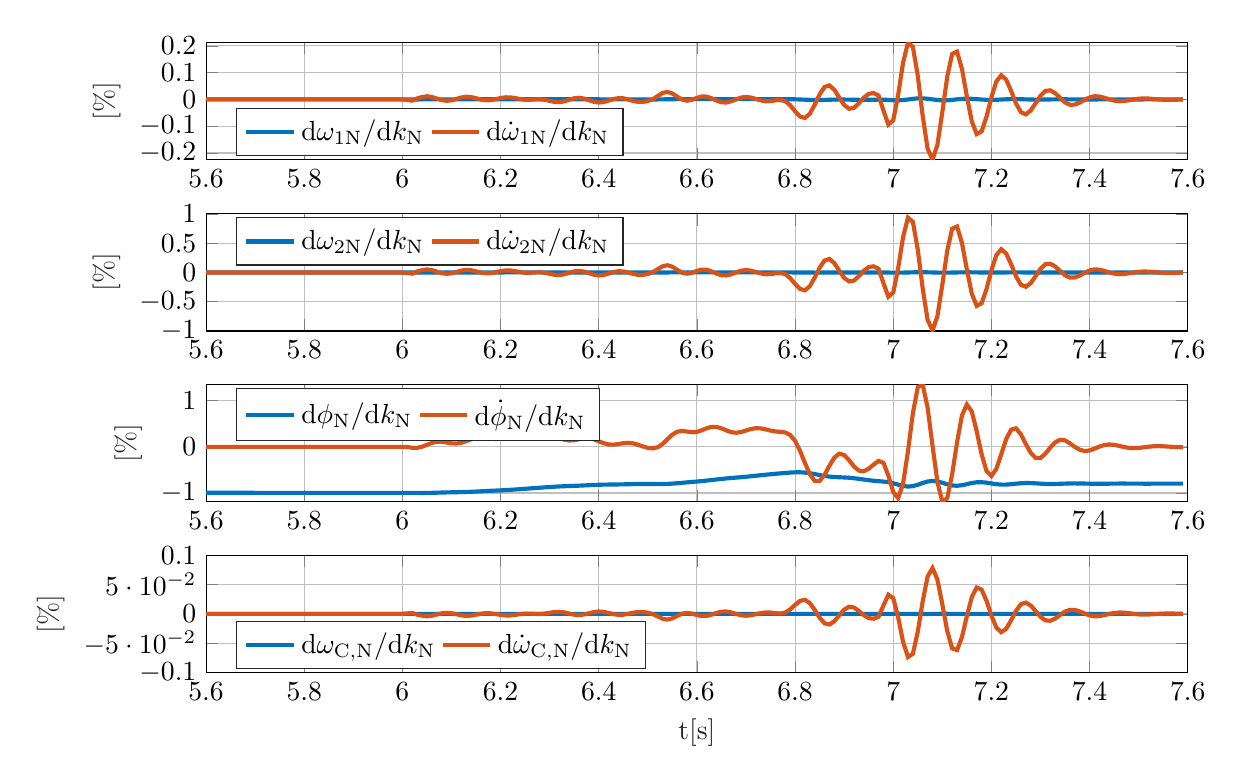
\begin{tikzpicture}

\begin{axis}[%
width=0.959\kwidth,
height=0.186\kheight,
at={(0\kwidth,0.814\kheight)},
scale only axis,
xmin=5.6,
xmax=7.6,
ymin=-0.224972743437563,
ymax=0.21217971045935,
ylabel style={font=\color{white!15!black}},
ylabel={[$\%$]},
axis background/.style={fill=white},
xmajorgrids,
ymajorgrids,
legend style={at={(0.03,0.03)}, anchor=south west, legend columns=2, legend cell align=left, align=left, draw=white!15!black}
]
\addplot [color=mycolor1, line width=1.5pt]
  table[row sep=crcr]{%
5.59	0\\
5.6	-1.41510818410119e-09\\
5.61	-2.83211022599453e-09\\
5.62	-4.25107476242952e-09\\
5.63	-5.67199831434385e-09\\
5.64	-7.09489033096427e-09\\
5.65	-8.51969595583294e-09\\
5.66	-9.94640600789955e-09\\
5.67	-1.13749817160169e-08\\
5.68	-1.28054484793402e-08\\
5.69	-1.42377976534863e-08\\
5.7	-1.56720653815931e-08\\
5.71	-1.71069091886835e-08\\
5.72	-1.85385740825006e-08\\
5.73	-1.99655111610592e-08\\
5.74	-2.13926624578532e-08\\
5.75	-2.28293572385806e-08\\
5.76	-2.42829561286085e-08\\
5.77	-2.5752815584753e-08\\
5.78	-2.72293360056864e-08\\
5.79	-2.86987669717368e-08\\
5.8	-3.015105514597e-08\\
5.81	-3.15852259367868e-08\\
5.82	-3.30102134116213e-08\\
5.83	-3.44394702285766e-08\\
5.84	-3.58842599787627e-08\\
5.85	-3.73476528841186e-08\\
5.86	-3.88240159966859e-08\\
5.87	-4.03018586803586e-08\\
5.88	-4.1770369952081e-08\\
5.89	-4.32230900248886e-08\\
5.9	-4.46608885967909e-08\\
5.91	-4.60879907389399e-08\\
5.92	-4.74884614432284e-08\\
5.93	-4.78457760548227e-08\\
5.94	-2.98893529506199e-08\\
5.95	9.11131624258556e-08\\
5.96	4.52820908434895e-07\\
5.97	1.09380359149309e-06\\
5.98	1.81273420611065e-06\\
5.99	2.21138653925926e-06\\
6	1.91029849737078e-06\\
6.01	-5.90003171112041e-06\\
6.02	-5.87230347430544e-05\\
6.03	-6.24647671892875e-05\\
6.04	1.02810971665611e-05\\
6.05	0.000134599941454043\\
6.06	0.000258825071032956\\
6.07	0.000331855670471403\\
6.08	0.000333379465583556\\
6.09	0.000283268633617921\\
6.1	0.000229009453418834\\
6.11	0.000218084221085593\\
6.12	0.000271458190607325\\
6.13	0.000374332443863165\\
6.14	0.000485844146523988\\
6.15	0.000562960223125676\\
6.16	0.000584154235898837\\
6.17	0.000559350049510993\\
6.18	0.000522702969557048\\
6.19	0.000511708869144276\\
6.2	0.000546837469984502\\
6.21	0.000623967534252785\\
6.22	0.000716180715924012\\
6.23	0.000790365977069462\\
6.24	0.000826223028969101\\
6.25	0.000824839264730356\\
6.26	0.000807977551744242\\
6.27	0.000800004569777659\\
6.28	0.000805098847834069\\
6.29	0.000802741958286084\\
6.3	0.000765651890152413\\
6.31	0.000680601820589695\\
6.32	0.000565174463688821\\
6.33	0.000461970062809105\\
6.34	0.000412631874015853\\
6.35	0.000431190360060187\\
6.36	0.000494277608097409\\
6.37	0.000552832929033487\\
6.38	0.000557227797254742\\
6.39	0.000487993743371917\\
6.4	0.00036505647919851\\
6.41	0.000239365926028247\\
6.42	0.000156300367073396\\
6.43	0.000144343715803345\\
6.44	0.000183024887243903\\
6.45	0.000238143785186935\\
6.46	0.000262820214315627\\
6.47	0.000228722863973761\\
6.48	0.000139755904637312\\
6.49	2.91335553746239e-05\\
6.5	-6.07015075128523e-05\\
6.51	-9.51156669477822e-05\\
6.52	-2.32289398851743e-05\\
6.53	0.000189536317003794\\
6.54	0.000498226796050502\\
6.55	0.000793913146445559\\
6.56	0.000980834223625734\\
6.57	0.00102963735807379\\
6.58	0.000988986419001687\\
6.59	0.000947383420563316\\
6.6	0.000972456844936264\\
6.61	0.00107438971883725\\
6.62	0.00120474303473293\\
6.63	0.00129316359516816\\
6.64	0.00129115075164037\\
6.65	0.00119927099578909\\
6.66	0.00106470096639387\\
6.67	0.00095333727636052\\
6.68	0.000915073487915299\\
6.69	0.000959832706802379\\
6.7	0.00105713812867133\\
6.71	0.00115499803735368\\
6.72	0.00120734880712917\\
6.73	0.00119522031192428\\
6.74	0.00113190804068504\\
6.75	0.00105287235504871\\
6.76	0.000997012833927804\\
6.77	0.000971632732904428\\
6.78	0.000930532902970461\\
6.79	0.000772202778340541\\
6.8	0.000386869398761244\\
6.81	-0.000246591413362375\\
6.82	-0.00103089454613994\\
6.83	-0.00175847817622117\\
6.84	-0.00219336693900351\\
6.85	-0.002197524082868\\
6.86	-0.00180646776112603\\
6.87	-0.00121601059939178\\
6.88	-0.000689912905576455\\
6.89	-0.000437837892161299\\
6.9	-0.000525049595865987\\
6.91	-0.000861594038741148\\
6.92	-0.00125943599179244\\
6.93	-0.001531920397184\\
6.94	-0.00157735034073747\\
6.95	-0.00141187184578622\\
6.96	-0.00114308584434848\\
6.97	-0.000907995527179683\\
6.98	-0.00102458307035628\\
6.99	-0.00184771278295917\\
7	-0.0029143042589184\\
7.01	-0.00330886236596755\\
7.02	-0.00236980842682055\\
7.03	-0.000282555446898104\\
7.04	0.00216965204655618\\
7.05	0.00385986696007608\\
7.06	0.00402314779243527\\
7.07	0.00253199165303286\\
7.08	8.43349131782456e-05\\
7.09	-0.00225773359049925\\
7.1	-0.00354186043499488\\
7.11	-0.00331284195739565\\
7.12	-0.00176971474741092\\
7.13	0.000293372834088028\\
7.14	0.00203549653694648\\
7.15	0.00273727841485548\\
7.16	0.00228792653601669\\
7.17	0.00101100928910936\\
7.18	-0.000471147939066833\\
7.19	-0.0015520535957586\\
7.2	-0.00187882977492344\\
7.21	-0.00142201605459732\\
7.22	-0.000478686662189232\\
7.23	0.000491609324333917\\
7.24	0.00111649381119821\\
7.25	0.00119856577815556\\
7.26	0.00081546335148376\\
7.27	0.000194209350691157\\
7.28	-0.000379777644656552\\
7.29	-0.000711287705148605\\
7.3	-0.000710601020493013\\
7.31	-0.000435226798973733\\
7.32	-4.16683150502939e-05\\
7.33	0.000294135122046647\\
7.34	0.000460308037147069\\
7.35	0.000423250037506446\\
7.36	0.000232363772565022\\
7.37	-2.01363819877364e-06\\
7.38	-0.000186749276278328\\
7.39	-0.000265573798452746\\
7.4	-0.000230060745644579\\
7.41	-0.000114525498299625\\
7.42	1.98828390996805e-05\\
7.43	0.000117373225095179\\
7.44	0.000156043180195133\\
7.45	0.000132926136836801\\
7.46	6.84641656151856e-05\\
7.47	-6.3445518168707e-06\\
7.48	-6.07089610188345e-05\\
7.49	-8.07731976043378e-05\\
7.5	-6.5742095396219e-05\\
7.51	-2.79232021520672e-05\\
7.52	1.26287702168297e-05\\
7.53	4.04975646500683e-05\\
7.54	5.04428314827405e-05\\
7.55	4.12615693519923e-05\\
7.56	2.13554850984906e-05\\
7.57	3.58969770749077e-07\\
7.58	-1.4705852285178e-05\\
7.59	-1.99259078089042e-05\\
};
\addlegendentry{d$\omega_{1\mathrm{N}}/$d$k_\mathrm{N}$}

\addplot [color=mycolor2, line width=1.5pt]
  table[row sep=crcr]{%
5.59	-1.22635341523205e-07\\
5.6	-1.22789333037663e-07\\
5.61	-1.22964392527965e-07\\
5.62	-1.2312644727569e-07\\
5.63	-1.23305636893318e-07\\
5.64	-1.23466370399666e-07\\
5.65	-1.23640508681875e-07\\
5.66	-1.23795693640055e-07\\
5.67	-1.23966562432268e-07\\
5.68	-1.24121654204658e-07\\
5.69	-1.24294638314299e-07\\
5.7	-1.24452089018396e-07\\
5.71	-1.24415449031465e-07\\
5.72	-1.24020363248e-07\\
5.73	-1.23661316403122e-07\\
5.74	-1.23912176542899e-07\\
5.75	-1.25038783422816e-07\\
5.76	-1.26619304940903e-07\\
5.77	-1.27872860153469e-07\\
5.78	-1.28055639420843e-07\\
5.79	-1.27051637084545e-07\\
5.8	-1.25372720691025e-07\\
5.81	-1.23941912128419e-07\\
5.82	-1.23506673253748e-07\\
5.83	-1.24290368408288e-07\\
5.84	-1.25863572845039e-07\\
5.85	-1.27433384653428e-07\\
5.86	-1.28270711558053e-07\\
5.87	-1.28033903835375e-07\\
5.88	-1.26945287470727e-07\\
5.89	-1.25488971960619e-07\\
5.9	-1.24288353598391e-07\\
5.91	-1.2351810848138e-07\\
5.92	-1.12729304016842e-07\\
5.93	1.7031952920919e-07\\
5.94	4.11188391309549e-06\\
5.95	1.91650337144868e-05\\
5.96	4.44981854696812e-05\\
5.97	6.37967529259631e-05\\
5.98	5.49208585717798e-05\\
5.99	9.09915005081205e-06\\
6	-5.55639699437093e-05\\
6.01	-0.00224817285270803\\
6.02	-0.00464371686661228\\
6.03	0.00377941320726706\\
6.04	0.00874552713152787\\
6.05	0.0118117082208911\\
6.06	0.00902747434412924\\
6.07	0.00328536080778647\\
6.08	-0.00270322288181152\\
6.09	-0.00527857558079848\\
6.1	-0.00339104972563535\\
6.11	0.00181461761669281\\
6.12	0.00723937419818908\\
6.13	0.00999028257106491\\
6.14	0.00869558536425857\\
6.15	0.00434510899290308\\
6.16	-0.000529689184230599\\
6.17	-0.00327327302950851\\
6.18	-0.00257355683878237\\
6.19	0.000891180812800641\\
6.2	0.00514046416703627\\
6.21	0.00784686523417278\\
6.22	0.00765960803003514\\
6.23	0.0049379699344998\\
6.24	0.00130364762307132\\
6.25	-0.00121895206071957\\
6.26	-0.0013321244814459\\
6.27	2.18724618319371e-05\\
6.28	0.000590491346923223\\
6.29	-0.00131263944482456\\
6.3	-0.0053359505467878\\
6.31	-0.00920708404986193\\
6.32	-0.0101767805251987\\
6.33	-0.00707911569535224\\
6.34	-0.00125066163546802\\
6.35	0.00416144201110057\\
6.36	0.00609793799610382\\
6.37	0.00327831530212434\\
6.38	-0.00282944338675044\\
6.39	-0.00891017568305275\\
6.4	-0.0116651161983099\\
6.41	-0.00978351012315971\\
6.42	-0.0044308332092262\\
6.43	0.00143577327603107\\
6.44	0.00478619113315388\\
6.45	0.00407259245359891\\
6.46	-0.00023453989757352\\
6.47	-0.00565623330923237\\
6.48	-0.00927162558977278\\
6.49	-0.00926916976871049\\
6.5	-0.0058836726674514\\
6.51	0.00067286975268619\\
6.52	0.0123543404620528\\
6.53	0.0239337538199492\\
6.54	0.0280347052428536\\
6.55	0.0219956311054841\\
6.56	0.0100167107720241\\
6.57	-0.00083073352490328\\
6.58	-0.00484901873393564\\
6.59	-0.00131015510348652\\
6.6	0.00586951604833837\\
6.61	0.0110617959954275\\
6.62	0.0104617285888451\\
6.63	0.00413060532353322\\
6.64	-0.00447267513036478\\
6.65	-0.0107402181191039\\
6.66	-0.0115916186454235\\
6.67	-0.00695301375010392\\
6.68	0.000462431775813528\\
6.69	0.00683535134674297\\
6.7	0.00924999465327533\\
6.71	0.0070246494554386\\
6.72	0.00177343234654852\\
6.73	-0.00367358771930096\\
6.74	-0.00677788069325921\\
6.75	-0.00645962305710979\\
6.76	-0.00348521502443091\\
6.77	-0.00173725903261249\\
6.78	-0.00662446582378797\\
6.79	-0.021789921456322\\
6.8	-0.0442536899709438\\
6.81	-0.0639022209263738\\
6.82	-0.0691957599825655\\
6.83	-0.0534248364495007\\
6.84	-0.0198634653246719\\
6.85	0.0186346765520778\\
6.86	0.0462425843211938\\
6.87	0.0521696088297782\\
6.88	0.0358834113149898\\
6.89	0.00687222193071706\\
6.9	-0.0206713246733927\\
6.91	-0.034847562708523\\
6.92	-0.0313369807015244\\
6.93	-0.0144125590240677\\
6.94	0.00624771860196\\
6.95	0.0208006347167476\\
6.96	0.0237637218859442\\
6.97	0.0143208030714703\\
6.98	-0.0409156929030654\\
6.99	-0.0940027173178763\\
7	-0.0777517209787355\\
7.01	0.0164612027651488\\
7.02	0.13664527684795\\
7.03	0.21217971045935\\
7.04	0.196191359881584\\
7.05	0.0882034651226782\\
7.06	-0.0614856405602748\\
7.07	-0.183579626911399\\
7.08	-0.224972743437563\\
7.09	-0.169133978734577\\
7.1	-0.0477030349936766\\
7.11	0.0844350711488333\\
7.12	0.169301802387234\\
7.13	0.178184726929368\\
7.14	0.114121039019849\\
7.15	0.0114372914320584\\
7.16	-0.0816645663494867\\
7.17	-0.129450641471558\\
7.18	-0.119607979240661\\
7.19	-0.0643936213375556\\
7.2	0.00794929632451692\\
7.21	0.0668848287256736\\
7.22	0.0899202832222946\\
7.23	0.073893944881823\\
7.24	0.0325758000322384\\
7.25	-0.0143352240358005\\
7.26	-0.0472482269714299\\
7.27	-0.0555529875959031\\
7.28	-0.0415905795345556\\
7.29	-0.0143470900716358\\
7.3	0.0138587641958214\\
7.31	0.031939277636061\\
7.32	0.0337323474241667\\
7.33	0.0229899289376286\\
7.34	0.00542724127733901\\
7.35	-0.0110682310885361\\
7.36	-0.0199256701897168\\
7.37	-0.0193791225586498\\
7.38	-0.0119954653569892\\
7.39	-0.00158840162234509\\
7.4	0.00743736737316481\\
7.41	0.0120439632695942\\
7.42	0.0108723738298291\\
7.43	0.00627648115611349\\
7.44	0.000466768160670286\\
7.45	-0.00437185066796705\\
7.46	-0.00672223038917232\\
7.47	-0.00598779683502517\\
7.48	-0.00337980440087624\\
7.49	-0.000111967990074198\\
7.5	0.00255298385531631\\
7.51	0.00374917793787559\\
7.52	0.00321458363374161\\
7.53	0.00174196443204695\\
7.54	1.80958067727146e-06\\
7.55	-0.00135033031896133\\
7.56	-0.00190353074431886\\
7.57	-0.00165798055415354\\
7.58	-0.000914036091115004\\
7.59	5.40671687017413e-06\\
};
\addlegendentry{d$\dot{\omega}_{1\mathrm{N}}/$d$k_\mathrm{N}$}

\end{axis}

\begin{axis}[%
width=0.959\kwidth,
height=0.186\kheight,
at={(0\kwidth,0.542\kheight)},
scale only axis,
xmin=5.6,
xmax=7.6,
ymin=-1,
ymax=1,
ylabel style={font=\color{white!15!black}},
ylabel={[$\%$]},
axis background/.style={fill=white},
xmajorgrids,
ymajorgrids,
legend style={at={(0.03,0.97)}, anchor=north west, legend columns=2, legend cell align=left, align=left, draw=white!15!black}
]
\addplot [color=mycolor1, line width=1.5pt]
  table[row sep=crcr]{%
5.59	0\\
5.6	-1.33015633057107e-09\\
5.61	-2.66209282422508e-09\\
5.62	-3.99587401274102e-09\\
5.63	-5.33149661228769e-09\\
5.64	-6.66896949949222e-09\\
5.65	-8.00824111654206e-09\\
5.66	-9.34930283834446e-09\\
5.67	-1.06921182163087e-08\\
5.68	-1.20367111249155e-08\\
5.69	-1.33830734371033e-08\\
5.7	-1.47312391297255e-08\\
5.71	-1.60799463191955e-08\\
5.72	-1.74256654367211e-08\\
5.73	-1.87669405542499e-08\\
5.74	-2.01084170257764e-08\\
5.75	-2.14588640668393e-08\\
5.76	-2.28252004361773e-08\\
5.77	-2.42068212209605e-08\\
5.78	-2.55947030890185e-08\\
5.79	-2.69759210955074e-08\\
5.8	-2.83410254236334e-08\\
5.81	-2.96890999961061e-08\\
5.82	-3.10285425471641e-08\\
5.83	-3.23719981374439e-08\\
5.84	-3.37300541979671e-08\\
5.85	-3.51055966267237e-08\\
5.86	-3.64933306360821e-08\\
5.87	-3.78824553829616e-08\\
5.88	-3.92628089050065e-08\\
5.89	-4.06283192080911e-08\\
5.9	-4.19798037770963e-08\\
5.91	-4.33212340497476e-08\\
5.92	-4.46376316254021e-08\\
5.93	-4.4973495947995e-08\\
5.94	-2.80950344421438e-08\\
5.95	8.5643451218963e-08\\
5.96	4.25637140860066e-07\\
5.97	1.02814031884011e-06\\
5.98	1.70391205363096e-06\\
5.99	2.07863246987296e-06\\
6	1.79561940630159e-06\\
6.01	-5.54584084559992e-06\\
6.02	-5.51977706543112e-05\\
6.03	-5.87148791204755e-05\\
6.04	9.66390130262211e-06\\
6.05	0.000126519629724644\\
6.06	0.000243287269500737\\
6.07	0.000311933691991007\\
6.08	0.000313366009641946\\
6.09	0.000266263433449914\\
6.1	0.000215261543256064\\
6.11	0.000204992175511245\\
6.12	0.000255161995960361\\
6.13	0.000351860498754404\\
6.14	0.00045667792477025\\
6.15	0.000529164564524863\\
6.16	0.00054908625713436\\
6.17	0.000525771117034574\\
6.18	0.000491324036598753\\
6.19	0.000480989928498157\\
6.2	0.000514009686888929\\
6.21	0.000586509476912091\\
6.22	0.000673186911802139\\
6.23	0.00074291868116743\\
6.24	0.000776623160437857\\
6.25	0.000775322466277559\\
6.26	0.000759472996983132\\
6.27	0.000751978649405423\\
6.28	0.000756767107740533\\
6.29	0.000754551713212825\\
6.3	0.000719688238678575\\
6.31	0.000639743896032505\\
6.32	0.000531245880665005\\
6.33	0.000434237052029055\\
6.34	0.000387860736370007\\
6.35	0.000405305118363346\\
6.36	0.000464605114699754\\
6.37	0.000519645241222021\\
6.38	0.000523776276408957\\
6.39	0.000458698482583818\\
6.4	0.000343141394669434\\
6.41	0.000224996303676501\\
6.42	0.000146917335387067\\
6.43	0.000135678460863445\\
6.44	0.000172037524346685\\
6.45	0.000223847520934082\\
6.46	0.000247042573277865\\
6.47	0.000214992154478387\\
6.48	0.000131366064452263\\
6.49	2.73846016385524e-05\\
6.5	-5.70574778310177e-05\\
6.51	-8.94056846496611e-05\\
6.52	-2.1834465573126e-05\\
6.53	0.000178158056187191\\
6.54	0.000468317212013852\\
6.55	0.000746252900392004\\
6.56	0.000921952718088834\\
6.57	0.000967826106502415\\
6.58	0.000929615528356809\\
6.59	0.000890510043303468\\
6.6	0.000914078252046739\\
6.61	0.00100989188565203\\
6.62	0.00113241982432728\\
6.63	0.00121553231685755\\
6.64	0.00121364030924541\\
6.65	0.00112727628387954\\
6.66	0.00100078476983967\\
6.67	0.000896106469379912\\
6.68	0.000860139734797667\\
6.69	0.000902211965386805\\
6.7	0.000993675942732279\\
6.71	0.0010856611202929\\
6.72	0.0011348691657932\\
6.73	0.00112346876926733\\
6.74	0.0010639572645986\\
6.75	0.000989666253553964\\
6.76	0.000937160100695444\\
6.77	0.000913303621423081\\
6.78	0.000874671097167241\\
6.79	0.000725845847487868\\
6.8	0.000363644809284718\\
6.81	-0.000231788052349322\\
6.82	-0.000969007847388172\\
6.83	-0.00165291313221928\\
6.84	-0.00206169463218205\\
6.85	-0.00206560221576993\\
6.86	-0.00169802181048079\\
6.87	-0.00114301100562374\\
6.88	-0.000648496033317605\\
6.89	-0.000411553600981826\\
6.9	-0.000493529806837052\\
6.91	-0.000809870794351703\\
6.92	-0.00118382947760308\\
6.93	-0.0014399560842565\\
6.94	-0.00148265877436122\\
6.95	-0.00132711429348259\\
6.96	-0.00107446406800422\\
6.97	-0.000853486705662627\\
6.98	-0.000963075260691388\\
6.99	-0.0017367908063854\\
7	-0.00273935259977096\\
7.01	-0.00311022456854624\\
7.02	-0.00222754395434538\\
7.03	-0.000265593055529859\\
7.04	0.00203940338259758\\
7.05	0.00362815121473031\\
7.06	0.0037816299543196\\
7.07	0.0023799909693852\\
7.08	7.92720949092305e-05\\
7.09	-0.0021221972222163\\
7.1	-0.00332923529331734\\
7.11	-0.00311396526115414\\
7.12	-0.00166347514129187\\
7.13	0.000275761051955867\\
7.14	0.00191330148563254\\
7.15	0.00257295395369206\\
7.16	0.00215057758312285\\
7.17	0.000950316297088581\\
7.18	-0.000442863976775874\\
7.19	-0.00145888063927896\\
7.2	-0.00176603976756004\\
7.21	-0.00133664951798332\\
7.22	-0.000449950126806306\\
7.23	0.000462096997222823\\
7.24	0.00104946837964689\\
7.25	0.00112661338728854\\
7.26	0.000766509385533384\\
7.27	0.000182550538931238\\
7.28	-0.000356978837430437\\
7.29	-0.000668587668131151\\
7.3	-0.000667942206530046\\
7.31	-0.000409099279573371\\
7.32	-3.91669184331171e-05\\
7.33	0.000276477545486377\\
7.34	0.000432674756641473\\
7.35	0.000397841425293587\\
7.36	0.000218414454686121\\
7.37	-1.89279852208668e-06\\
7.38	-0.000175538375970664\\
7.39	-0.000249630899420124\\
7.4	-0.000216249768117066\\
7.41	-0.000107650339207808\\
7.42	1.86891895215344e-05\\
7.43	0.000110327024222188\\
7.44	0.000146675539057642\\
7.45	0.000124946259265637\\
7.46	6.43540795985222e-05\\
7.47	-5.9637168161943e-06\\
7.48	-5.706451857294e-05\\
7.49	-7.59242570645237e-05\\
7.5	-6.1795502909978e-05\\
7.51	-2.6246955547581e-05\\
7.52	1.18705985957657e-05\\
7.53	3.8066370651726e-05\\
7.54	4.74146019697137e-05\\
7.55	3.87845094399457e-05\\
7.56	2.00734280784362e-05\\
7.57	3.37376760089678e-07\\
7.58	-1.38230730696614e-05\\
7.59	-1.87297576471503e-05\\
};
\addlegendentry{d$\omega_{2\mathrm{N}}/$d$k_\mathrm{N}$}

\addplot [color=mycolor2, line width=1.5pt]
  table[row sep=crcr]{%
5.59	-5.40347141142244e-07\\
5.6	-5.41025646688087e-07\\
5.61	-5.41796980671062e-07\\
5.62	-5.42511015193301e-07\\
5.63	-5.43300553520013e-07\\
5.64	-5.44008761138775e-07\\
5.65	-5.44776037099686e-07\\
5.66	-5.45459799628658e-07\\
5.67	-5.46212671503091e-07\\
5.68	-5.46896027283931e-07\\
5.69	-5.47658216528372e-07\\
5.7	-5.4835196094029e-07\\
5.71	-5.48190522133603e-07\\
5.72	-5.46449722895727e-07\\
5.73	-5.44867723331306e-07\\
5.74	-5.45973042462408e-07\\
5.75	-5.5093701795275e-07\\
5.76	-5.57901000022743e-07\\
5.77	-5.63424327504302e-07\\
5.78	-5.64229672252622e-07\\
5.79	-5.59805910307943e-07\\
5.8	-5.5240838438999e-07\\
5.81	-5.46104060292499e-07\\
5.82	-5.44186344535575e-07\\
5.83	-5.47639404427252e-07\\
5.84	-5.54571144613313e-07\\
5.85	-5.61487936805512e-07\\
5.86	-5.65177305538001e-07\\
5.87	-5.64133901985975e-07\\
5.88	-5.59337319905791e-07\\
5.89	-5.5292060562378e-07\\
5.9	-5.47630524547968e-07\\
5.91	-5.44236726913246e-07\\
5.92	-4.96699857489174e-07\\
5.93	7.50449819370114e-07\\
5.94	1.81174910917716e-05\\
5.95	8.44436114934479e-05\\
5.96	0.000196064746975298\\
5.97	0.000281096725374478\\
5.98	0.00024198838955349\\
5.99	4.00920292272454e-05\\
6	-0.000244822021244322\\
6.01	-0.00990573968087529\\
6.02	-0.0204608157139387\\
6.03	0.0166525822658743\\
6.04	0.0385339210161533\\
6.05	0.0520439105389991\\
6.06	0.0397762168157874\\
6.07	0.0144757236439628\\
6.08	-0.01191074882625\\
6.09	-0.0232580851273155\\
6.1	-0.0149414026535296\\
6.11	0.00799543936741058\\
6.12	0.0318976168461853\\
6.13	0.0440184740991353\\
6.14	0.0383138711453554\\
6.15	0.0191451108916618\\
6.16	-0.0023338788938941\\
6.17	-0.0144224633331388\\
6.18	-0.0113394235092762\\
6.19	0.00392665765426027\\
6.2	0.0226495484171397\\
6.21	0.0345743007380235\\
6.22	0.0337492213339552\\
6.23	0.0217573326998383\\
6.24	0.00574403964275829\\
6.25	-0.00537086006639248\\
6.26	-0.00586951235525823\\
6.27	9.63728891288343e-05\\
6.28	0.00260178106829535\\
6.29	-0.00578365876966298\\
6.3	-0.023510886630813\\
6.31	-0.0405676003550986\\
6.32	-0.0448402081497231\\
6.33	-0.0311914972038143\\
6.34	-0.00551057654436103\\
6.35	0.0183358504704609\\
6.36	0.0268683016551594\\
6.37	0.0144446802369069\\
6.38	-0.0124668926578134\\
6.39	-0.0392593837795167\\
6.4	-0.0513980071720884\\
6.41	-0.0431074080128938\\
6.42	-0.0195228228501621\\
6.43	0.0063262023184614\\
6.44	0.0210885757164073\\
6.45	0.0179443678554521\\
6.46	-0.00103341305244878\\
6.47	-0.0249220938096688\\
6.48	-0.040851978708026\\
6.49	-0.0408411580435455\\
6.5	-0.0259242209694998\\
6.51	0.00296475095374552\\
6.52	0.0544348182118391\\
6.53	0.105455207610438\\
6.54	0.123524528743937\\
6.55	0.0969155888458278\\
6.56	0.0441349201627145\\
6.57	-0.00366031910400192\\
6.58	-0.0213654022323839\\
6.59	-0.00577271244116281\\
6.6	0.0258618450789914\\
6.61	0.0487397005090691\\
6.62	0.046095726086275\\
6.63	0.0181999800460374\\
6.64	-0.0197071837537471\\
6.65	-0.0473227868913512\\
6.66	-0.051074167470351\\
6.67	-0.0306358757615543\\
6.68	0.0020375340738813\\
6.69	0.0301174400298303\\
6.7	0.0407566700106794\\
6.71	0.0309515119227254\\
6.72	0.00781397175282991\\
6.73	-0.0161863015107628\\
6.74	-0.0298642169148859\\
6.75	-0.0284619327038019\\
6.76	-0.0153563071105916\\
6.77	-0.00765458746402939\\
6.78	-0.0291882512041857\\
6.79	-0.0960092055879843\\
6.8	-0.194987468264346\\
6.81	-0.281561430992162\\
6.82	-0.304885447122861\\
6.83	-0.235396723043087\\
6.84	-0.0875209912926456\\
6.85	0.0821067894044574\\
6.86	0.203750793407515\\
6.87	0.229866028182928\\
6.88	0.158106940451561\\
6.89	0.030279896580396\\
6.9	-0.0910805238248306\\
6.91	-0.153542857831271\\
6.92	-0.138074780522273\\
6.93	-0.063503594777261\\
6.94	0.027528254331423\\
6.95	0.0916502805613007\\
6.96	0.104706024969228\\
6.97	0.0630993062104326\\
6.98	-0.180279822466525\\
6.99	-0.414188102095359\\
7	-0.34258411528606\\
7.01	0.0725301834461671\\
7.02	0.602076721745827\\
7.03	0.93489118278486\\
7.04	0.864444447090542\\
7.05	0.388635848619757\\
7.06	-0.27091366607691\\
7.07	-0.808875524275363\\
7.08	-0.991258936829371\\
7.09	-0.745226134421427\\
7.1	-0.210185727518985\\
7.11	0.372031818518198\\
7.12	0.745965587090069\\
7.13	0.785104898826355\\
7.14	0.502832023471652\\
7.15	0.0503941818547295\\
7.16	-0.359824616881602\\
7.17	-0.570376229921332\\
7.18	-0.527008190089089\\
7.19	-0.283726604611434\\
7.2	0.0350256253392278\\
7.21	0.294703185815156\\
7.22	0.396200370695418\\
7.23	0.325586256016881\\
7.24	0.14353317834382\\
7.25	-0.0631628468400764\\
7.26	-0.208181784687045\\
7.27	-0.244773631599035\\
7.28	-0.183253460048513\\
7.29	-0.063215130125094\\
7.3	0.0610635033053745\\
7.31	0.140728578532917\\
7.32	0.148629075387163\\
7.33	0.101296593392969\\
7.34	0.0239131253692682\\
7.35	-0.0487680543596597\\
7.36	-0.0877950739546039\\
7.37	-0.0853869145686296\\
7.38	-0.0528535681916676\\
7.39	-0.00699870250665374\\
7.4	0.0327700003230763\\
7.41	0.053067256252503\\
7.42	0.0479050820054475\\
7.43	0.0276549858563859\\
7.44	0.00205664074510184\\
7.45	-0.0192629381625944\\
7.46	-0.0296190144942702\\
7.47	-0.0263830054874391\\
7.48	-0.014891854301605\\
7.49	-0.000493345412000799\\
7.5	0.0112487762894961\\
7.51	0.0165193617675469\\
7.52	0.0141638702824215\\
7.53	0.00767532006108939\\
7.54	7.97324596008445e-06\\
7.55	-0.00594972962452983\\
7.56	-0.0083872020805912\\
7.57	-0.00730527625827759\\
7.58	-0.004027360959636\\
7.59	2.38226921791634e-05\\
};
\addlegendentry{d$\dot{\omega}_{2\mathrm{N}}/$d$k_\mathrm{N}$}

\end{axis}

\begin{axis}[%
width=0.959\kwidth,
height=0.186\kheight,
at={(0\kwidth,0.271\kheight)},
scale only axis,
xmin=5.6,
xmax=7.6,
ymin=-1.19110212790179,
ymax=1.34963966404923,
ylabel style={font=\color{white!15!black}},
ylabel={[$\%$]},
axis background/.style={fill=white},
xmajorgrids,
ymajorgrids,
legend style={at={(0.03,0.97)}, anchor=north west, legend columns=2, legend cell align=left, align=left, draw=white!15!black}
]
\addplot [color=mycolor1, line width=1.5pt]
  table[row sep=crcr]{%
5.59	-0.996957250189296\\
5.6	-0.996992415132887\\
5.61	-0.997027612653789\\
5.62	-0.997062842704039\\
5.63	-0.997098105350174\\
5.64	-0.997133400544444\\
5.65	-0.997168728353138\\
5.66	-0.9972040887279\\
5.67	-0.997239481734525\\
5.68	-0.997274907324379\\
5.69	-0.997310365563348\\
5.7	-0.997345856403002\\
5.71	-0.99738138016109\\
5.72	-0.997416936243568\\
5.73	-0.997452524900966\\
5.74	-0.997488146055747\\
5.75	-0.997523799815467\\
5.76	-0.997559486253119\\
5.77	-0.997595205578052\\
5.78	-0.9976309578214\\
5.79	-0.997666743009078\\
5.8	-0.997702560940233\\
5.81	-0.997738411489209\\
5.82	-0.997774294469339\\
5.83	-0.997810209924899\\
5.84	-0.997846157903421\\
5.85	-0.997882138624104\\
5.86	-0.99791815216539\\
5.87	-0.997954198628348\\
5.88	-0.997990277890666\\
5.89	-0.998026389868932\\
5.9	-0.998062534348738\\
5.91	-0.998098711262253\\
5.92	-0.998134918305013\\
5.93	-0.998171151818884\\
5.94	-0.998207351181705\\
5.95	-0.998243011821874\\
5.96	-0.998276497960404\\
5.97	-0.998305205064306\\
5.98	-0.998327239128487\\
5.99	-0.998343640401599\\
6	-0.998359590673015\\
6.01	-0.998395649317884\\
6.02	-0.998712046112471\\
6.03	-0.999403651524948\\
6.04	-0.999725015946947\\
6.05	-0.999091916776899\\
6.06	-0.997237366271996\\
6.07	-0.994421738394149\\
6.08	-0.991249584744953\\
6.09	-0.988339040440126\\
6.1	-0.985964108603792\\
6.11	-0.983929576451251\\
6.12	-0.981695454209934\\
6.13	-0.978698838581562\\
6.14	-0.974647522421155\\
6.15	-0.969674016812481\\
6.16	-0.964229550583132\\
6.17	-0.958820464192846\\
6.18	-0.95373539605055\\
6.19	-0.948893488565245\\
6.2	-0.943951132020963\\
6.21	-0.938466620213011\\
6.22	-0.932151694393709\\
6.23	-0.925028199221373\\
6.24	-0.91737174394931\\
6.25	-0.909562236308145\\
6.26	-0.90186960074121\\
6.27	-0.894298631140645\\
6.28	-0.886735252210645\\
6.29	-0.879142275652205\\
6.3	-0.871714660953681\\
6.31	-0.864864261828715\\
6.32	-0.858990365799808\\
6.33	-0.854191150935665\\
6.34	-0.850140338766964\\
6.35	-0.846233024898436\\
6.36	-0.841913187933786\\
6.37	-0.836968831433961\\
6.38	-0.831693621793434\\
6.39	-0.826724894115298\\
6.4	-0.822697896302445\\
6.41	-0.819883275743391\\
6.42	-0.818078980441621\\
6.43	-0.816751722571552\\
6.44	-0.81526341144587\\
6.45	-0.813305283186384\\
6.46	-0.810934447323017\\
6.47	-0.808597573049074\\
6.48	-0.806859975810304\\
6.49	-0.806100597418332\\
6.5	-0.806324585772554\\
6.51	-0.807166081719864\\
6.52	-0.807871392578058\\
6.53	-0.807224872017038\\
6.54	-0.804046616712797\\
6.55	-0.79789052594003\\
6.56	-0.789421361951509\\
6.57	-0.77983453559961\\
6.58	-0.770272516042628\\
6.59	-0.761170058667731\\
6.6	-0.752179961068685\\
6.61	-0.742571768488342\\
6.62	-0.731809242949415\\
6.63	-0.719957291290234\\
6.64	-0.707674091464958\\
6.65	-0.695859193251901\\
6.66	-0.685167623476578\\
6.67	-0.675692900738956\\
6.68	-0.666952570763296\\
6.69	-0.658172371719321\\
6.7	-0.648682768616073\\
6.71	-0.638225512027677\\
6.72	-0.627029008077227\\
6.73	-0.615640368724157\\
6.74	-0.604630514510092\\
6.75	-0.594327390880039\\
6.76	-0.584725754843209\\
6.77	-0.575471917673743\\
6.78	-0.566472559954361\\
6.79	-0.558355491291683\\
6.8	-0.552816629499457\\
6.81	-0.552085453371148\\
6.82	-0.558142106515459\\
6.83	-0.571543990199635\\
6.84	-0.590629263200606\\
6.85	-0.611841844829126\\
6.86	-0.631121541603439\\
6.87	-0.645549083439301\\
6.88	-0.654478388589162\\
6.89	-0.659603719481022\\
6.9	-0.663959532281686\\
6.91	-0.670447227421086\\
6.92	-0.68057912647565\\
6.93	-0.694010653150908\\
6.94	-0.708982561729515\\
6.95	-0.723328540654963\\
6.96	-0.735509501809746\\
6.97	-0.745192248239003\\
6.98	-0.753895799399296\\
6.99	-0.767095420333517\\
7	-0.789907822044014\\
7.01	-0.820347251133274\\
7.02	-0.848102726883417\\
7.03	-0.861217215016472\\
7.04	-0.852163496651187\\
7.05	-0.822506251685861\\
7.06	-0.783922074139568\\
7.07	-0.75205812871649\\
7.08	-0.739303991391649\\
7.09	-0.750356436379054\\
7.1	-0.778860340279091\\
7.11	-0.812492030380971\\
7.12	-0.837088027767858\\
7.13	-0.84418740780473\\
7.14	-0.832631404294647\\
7.15	-0.808930292598747\\
7.16	-0.784433781426801\\
7.17	-0.768688223080347\\
7.18	-0.766494543462567\\
7.19	-0.776725606063604\\
7.2	-0.793628791344897\\
7.21	-0.80986398843226\\
7.22	-0.818939250546755\\
7.23	-0.818479595668502\\
7.24	-0.810520724090499\\
7.25	-0.799156981441947\\
7.26	-0.789481044015627\\
7.27	-0.784966370466012\\
7.28	-0.786150710902592\\
7.29	-0.791599730437503\\
7.3	-0.798641898616267\\
7.31	-0.804308684455381\\
7.32	-0.806427175275006\\
7.33	-0.805182782656301\\
7.34	-0.801508932293794\\
7.35	-0.797213165773807\\
7.36	-0.794142186865927\\
7.37	-0.793225296419355\\
7.38	-0.794243272640301\\
7.39	-0.796502380300954\\
7.4	-0.798942534961662\\
7.41	-0.800645450499256\\
7.42	-0.800983509743478\\
7.43	-0.800283295967027\\
7.44	-0.798995225590926\\
7.45	-0.797654819604511\\
7.46	-0.796743841486269\\
7.47	-0.796563967274461\\
7.48	-0.79696281116033\\
7.49	-0.797700406062674\\
7.5	-0.798459535898908\\
7.51	-0.798957435741229\\
7.52	-0.79902497673139\\
7.53	-0.798786421895061\\
7.54	-0.798386997242606\\
7.55	-0.797989370732276\\
7.56	-0.797743316344936\\
7.57	-0.797699234079186\\
7.58	-0.797816025848558\\
7.59	-0.798030233392475\\
};
\addlegendentry{d$\phi_\mathrm{N}/$d$k_\mathrm{N}$}

\addplot [color=mycolor2, line width=1.5pt]
  table[row sep=crcr]{%
5.59	-0.00124521060538135\\
5.6	-0.00124636367383817\\
5.61	-0.00124751705169121\\
5.62	-0.00124867076247045\\
5.63	-0.00124982480431969\\
5.64	-0.00125097918088393\\
5.65	-0.00125213387305914\\
5.66	-0.00125328887823842\\
5.67	-0.00125444418271718\\
5.68	-0.00125559979550214\\
5.69	-0.00125675571300826\\
5.7	-0.00125791194785272\\
5.71	-0.0012590680458999\\
5.72	-0.00126022275164612\\
5.73	-0.00126137554180833\\
5.74	-0.00126252807663822\\
5.75	-0.00126368348868064\\
5.76	-0.00126484425038606\\
5.77	-0.00126601014479018\\
5.78	-0.00126717794822738\\
5.79	-0.00126834304193508\\
5.8	-0.00126950205010162\\
5.81	-0.00127065464492794\\
5.82	-0.00127180382757564\\
5.83	-0.00127295411550919\\
5.84	-0.00127410929203664\\
5.85	-0.00127527038746217\\
5.86	-0.00127643551029617\\
5.87	-0.0012776008006486\\
5.88	-0.00127876262817993\\
5.89	-0.00127991882282372\\
5.9	-0.00128106967732731\\
5.91	-0.00128221661015886\\
5.92	-0.00128335429190639\\
5.93	-0.00128414132756805\\
5.94	-0.00127877737158282\\
5.95	-0.00123880528117866\\
5.96	-0.00111799343337162\\
5.97	-0.000903390740406783\\
5.98	-0.000662615537309482\\
5.99	-0.000529412426000284\\
6	-0.000631219714250733\\
6.01	-0.00325501146874343\\
6.02	-0.0209961781283315\\
6.03	-0.0222528395476553\\
6.04	0.00217874500733993\\
6.05	0.0439303100206761\\
6.06	0.0856491382211162\\
6.07	0.110173110219721\\
6.08	0.110680902629155\\
6.09	0.093847296628966\\
6.1	0.0756210098939091\\
6.11	0.0719489364463447\\
6.12	0.0898717704870119\\
6.13	0.124418660446845\\
6.14	0.16186537485166\\
6.15	0.187759242152947\\
6.16	0.19487100129748\\
6.17	0.186534143137578\\
6.18	0.174220147247424\\
6.19	0.170522048390798\\
6.2	0.182314321416091\\
6.21	0.208212373357096\\
6.22	0.239175281493378\\
6.23	0.26408261141792\\
6.24	0.27611672560296\\
6.25	0.275643225542565\\
6.26	0.269971528680208\\
6.27	0.267285274462305\\
6.28	0.268987718076244\\
6.29	0.268187636478066\\
6.3	0.255722469957831\\
6.31	0.227150374063236\\
6.32	0.188376984831529\\
6.33	0.153709845066705\\
6.34	0.137134647746688\\
6.35	0.143362940305891\\
6.36	0.164545947272066\\
6.37	0.184206238804615\\
6.38	0.185676207998357\\
6.39	0.16241796810301\\
6.4	0.121124306297683\\
6.41	0.0789072156543156\\
6.42	0.051006938318475\\
6.43	0.0469893394644301\\
6.44	0.0599784663738735\\
6.45	0.0784877690586944\\
6.46	0.0867724301259812\\
6.47	0.0753177471038582\\
6.48	0.0454355444554813\\
6.49	0.00828133142367217\\
6.5	-0.0218903643511883\\
6.51	-0.0334481056093456\\
6.52	-0.00930446331885534\\
6.53	0.0621523077581373\\
6.54	0.165823240330577\\
6.55	0.265123558842331\\
6.56	0.327892247403441\\
6.57	0.344272371399013\\
6.58	0.33060906085245\\
6.59	0.316626487852106\\
6.6	0.325037548609827\\
6.61	0.359261483217289\\
6.62	0.403029313675928\\
6.63	0.432712739719884\\
6.64	0.43202334280892\\
6.65	0.40115232968493\\
6.66	0.355944831770619\\
6.67	0.318532556103185\\
6.68	0.305671922564643\\
6.69	0.320694822751097\\
6.7	0.353364808072293\\
6.71	0.386220005409636\\
6.72	0.403790025557858\\
6.73	0.399704263551907\\
6.74	0.37842865974093\\
6.75	0.351873047251418\\
6.76	0.333101983899238\\
6.77	0.324567914909334\\
6.78	0.310754594778694\\
6.79	0.257570005591963\\
6.8	0.128148305364871\\
6.81	-0.0846027738620303\\
6.82	-0.34800759214865\\
6.83	-0.592355201288185\\
6.84	-0.738394208776538\\
6.85	-0.739768248638883\\
6.86	-0.608410516913342\\
6.87	-0.410088461597645\\
6.88	-0.233387590885912\\
6.89	-0.148722238427989\\
6.9	-0.178008342807397\\
6.91	-0.291031469219605\\
6.92	-0.424637723215836\\
6.93	-0.516138713083362\\
6.94	-0.531381038623939\\
6.95	-0.475789696897654\\
6.96	-0.385504471614033\\
6.97	-0.306538719174204\\
6.98	-0.345686260059917\\
6.99	-0.622123707873449\\
7	-0.980318444275321\\
7.01	-1.11280032079523\\
7.02	-0.797386765198718\\
7.03	-0.0963621016789262\\
7.04	0.727210240357563\\
7.05	1.29484278400998\\
7.06	1.34963966404923\\
7.07	0.848795239629351\\
7.08	0.0267270891621329\\
7.09	-0.759853524127266\\
7.1	-1.19110212790179\\
7.11	-1.11415010260269\\
7.12	-0.595859683797049\\
7.13	0.0970425857728536\\
7.14	0.682128108715238\\
7.15	0.917798222246297\\
7.16	0.766855176156326\\
7.17	0.337980745405206\\
7.18	-0.15980977110087\\
7.19	-0.522825266470707\\
7.2	-0.632556601901608\\
7.21	-0.479117239691912\\
7.22	-0.162287537893674\\
7.23	0.163588788982103\\
7.24	0.373449426668214\\
7.25	0.401000929738659\\
7.26	0.272323793031988\\
7.27	0.063668143654277\\
7.28	-0.129106610186762\\
7.29	-0.240440064887664\\
7.3	-0.240202369707649\\
7.31	-0.14771138249859\\
7.32	-0.0155315957129218\\
7.33	0.0972473463431912\\
7.34	0.153052675874922\\
7.35	0.14060152389354\\
7.36	0.0764879249976148\\
7.37	-0.00223001324184151\\
7.38	-0.0642735083650856\\
7.39	-0.0907450495485913\\
7.4	-0.0788157206168461\\
7.41	-0.0400114498063924\\
7.42	0.0051299464916632\\
7.43	0.0378712008656061\\
7.44	0.0508567747892466\\
7.45	0.04309091400287\\
7.46	0.021439680271255\\
7.47	-0.00368575955982868\\
7.48	-0.0219442826725312\\
7.49	-0.0286826068838009\\
7.5	-0.0236340153819325\\
7.51	-0.010932345828467\\
7.52	0.0026867738796023\\
7.53	0.0120458730449383\\
7.54	0.015385119571432\\
7.55	0.0123006566703123\\
7.56	0.00561438879724362\\
7.57	-0.00143788548231614\\
7.58	-0.0064978056312354\\
7.59	-0.00825122068595814\\
};
\addlegendentry{d$\dot{\phi}_\mathrm{N}/$d$k_\mathrm{N}$}

\end{axis}

\begin{axis}[%
width=0.959\kwidth,
height=0.186\kheight,
at={(0\kwidth,0\kheight)},
scale only axis,
xmin=5.6,
xmax=7.6,
xlabel style={font=\color{white!15!black}},
xlabel={t[s]},
ymin=-0.1,
ymax=0.1,
ylabel style={font=\color{white!15!black}},
ylabel={[$\%$]},
axis background/.style={fill=white},
xmajorgrids,
ymajorgrids,
legend style={at={(0.03,0.03)}, anchor=south west, legend columns=2, legend cell align=left, align=left, draw=white!15!black}
]
\addplot [color=mycolor1, line width=1.5pt]
  table[row sep=crcr]{%
5.59	0\\
5.6	2.0042029116177e-09\\
5.61	4.007520343197e-09\\
5.62	6.0099558050792e-09\\
5.63	8.01150721347918e-09\\
5.64	1.00121762321082e-08\\
5.65	1.20119591752406e-08\\
5.66	1.40108571295773e-08\\
5.67	1.60088669138391e-08\\
5.68	1.8005990698492e-08\\
5.69	2.00022262436336e-08\\
5.7	2.19975760577721e-08\\
5.71	2.39919887915519e-08\\
5.72	2.59853634491138e-08\\
5.73	2.79776427705821e-08\\
5.74	2.996898238442e-08\\
5.75	3.19596715167759e-08\\
5.76	3.39499410425803e-08\\
5.77	3.59397684747206e-08\\
5.78	3.79288552080001e-08\\
5.79	3.99167700206077e-08\\
5.8	4.19032008282919e-08\\
5.81	4.38881158052977e-08\\
5.82	4.58717957355545e-08\\
5.83	4.78546587992872e-08\\
5.84	4.98370578319294e-08\\
5.85	5.1819086286331e-08\\
5.86	5.38005692923979e-08\\
5.87	5.57811459731573e-08\\
5.88	5.7760480366682e-08\\
5.89	5.97383692432275e-08\\
5.9	6.1714841661185e-08\\
5.91	6.36900279951228e-08\\
5.92	6.56634954803988e-08\\
5.93	6.76035260245392e-08\\
5.94	6.89709387400527e-08\\
5.95	6.71213519060108e-08\\
5.96	5.7761050918681e-08\\
5.97	3.9693404712271e-08\\
5.98	1.92107525313632e-08\\
5.99	8.74511770990162e-09\\
6	2.01302026663308e-08\\
6.01	2.65940236090644e-07\\
6.02	1.91649137219331e-06\\
6.03	2.03329547487426e-06\\
6.04	-2.37218195099188e-07\\
6.05	-4.11531236292886e-06\\
6.06	-7.98682947447374e-06\\
6.07	-1.02568596264297e-05\\
6.08	-1.02929352341138e-05\\
6.09	-8.71744146762796e-06\\
6.1	-7.0140194080432e-06\\
6.11	-6.66478002911165e-06\\
6.12	-8.32277162531584e-06\\
6.13	-1.15241906836625e-05\\
6.14	-1.49921659495088e-05\\
6.15	-1.73833320282604e-05\\
6.16	-1.8026853283192e-05\\
6.17	-1.72341364166996e-05\\
6.18	-1.60725924089913e-05\\
6.19	-1.57128351618209e-05\\
6.2	-1.67930247870392e-05\\
6.21	-1.91831413958755e-05\\
6.22	-2.20417575102401e-05\\
6.23	-2.4335004394082e-05\\
6.24	-2.54298099477725e-05\\
6.25	-2.53612745509539e-05\\
6.26	-2.48097862489234e-05\\
6.27	-2.45362395079642e-05\\
6.28	-2.46707707849299e-05\\
6.29	-2.45725534956105e-05\\
6.3	-2.33902604689595e-05\\
6.31	-2.07121107562365e-05\\
6.32	-1.70883529788356e-05\\
6.33	-1.3849530916416e-05\\
6.34	-1.22950220716811e-05\\
6.35	-1.28611162442375e-05\\
6.36	-1.48164381663853e-05\\
6.37	-1.66283636939616e-05\\
6.38	-1.67480672913129e-05\\
6.39	-1.45695508015386e-05\\
6.4	-1.07169437720459e-05\\
6.41	-6.78204248443047e-06\\
6.42	-4.18122943554634e-06\\
6.43	-3.80233422539874e-06\\
6.44	-5.00418474655153e-06\\
6.45	-6.71790313527583e-06\\
6.46	-7.47976828107954e-06\\
6.47	-6.40645461402622e-06\\
6.48	-3.6215908538981e-06\\
6.49	-1.6348428789788e-07\\
6.5	2.64252297673231e-06\\
6.51	3.71606411307244e-06\\
6.52	1.47063740464462e-06\\
6.53	-5.16979267502355e-06\\
6.54	-1.47979137246825e-05\\
6.55	-2.40109114501961e-05\\
6.56	-2.98205462172859e-05\\
6.57	-3.13138847419126e-05\\
6.58	-3.00139986274053e-05\\
6.59	-2.86858019031274e-05\\
6.6	-2.94400230362581e-05\\
6.61	-3.25924148471906e-05\\
6.62	-3.66287731181928e-05\\
6.63	-3.93524279623526e-05\\
6.64	-3.92508927859308e-05\\
6.65	-3.6344601512389e-05\\
6.66	-3.21087035847221e-05\\
6.67	-2.8601189746626e-05\\
6.68	-2.73785769887944e-05\\
6.69	-2.87483625380833e-05\\
6.7	-3.17568248640743e-05\\
6.71	-3.47796681959983e-05\\
6.72	-3.63791957468498e-05\\
6.73	-3.59647136797053e-05\\
6.74	-3.39531357575544e-05\\
6.75	-3.14527591655336e-05\\
6.76	-2.9678258409287e-05\\
6.77	-2.8856602227903e-05\\
6.78	-2.75448765652009e-05\\
6.79	-2.25752024168184e-05\\
6.8	-1.05249617780828e-05\\
6.81	9.25866131431859e-06\\
6.82	3.37317654860855e-05\\
6.83	5.6411272855279e-05\\
6.84	6.99336459985282e-05\\
6.85	6.99994002572064e-05\\
6.86	5.77300661265586e-05\\
6.87	3.92490786241044e-05\\
6.88	2.27946638683082e-05\\
6.89	1.49086294392044e-05\\
6.9	1.76196281866484e-05\\
6.91	2.81098405793721e-05\\
6.92	4.0502992488532e-05\\
6.93	4.89715996491536e-05\\
6.94	5.03454422266168e-05\\
6.95	4.51353454972122e-05\\
6.96	3.67060072164739e-05\\
6.97	2.93365483267631e-05\\
6.98	3.29517079535635e-05\\
6.99	5.86157727832517e-05\\
7	9.18527509458321e-05\\
7.01	0.000104081232575759\\
7.02	7.46742574334088e-05\\
7.03	9.45833391839681e-06\\
7.04	-6.70855848304743e-05\\
7.05	-0.000119771955045331\\
7.06	-0.000124750431855918\\
7.07	-7.80877330048685e-05\\
7.08	-1.61595067901296e-06\\
7.09	7.14853786992042e-05\\
7.1	0.000111497385727995\\
7.11	0.000104243730762173\\
7.12	5.59832414833221e-05\\
7.13	-8.45970101102456e-06\\
7.14	-6.28225937717779e-05\\
7.15	-8.46620328592284e-05\\
7.16	-7.05534247586332e-05\\
7.17	-3.06300749499761e-05\\
7.18	1.56602889322092e-05\\
7.19	4.93826817684822e-05\\
7.2	5.95358164624721e-05\\
7.21	4.52224410175501e-05\\
7.22	1.57391452444269e-05\\
7.23	-1.45567214070795e-05\\
7.24	-3.40434768695064e-05\\
7.25	-3.65696929672559e-05\\
7.26	-2.45754848134376e-05\\
7.27	-5.16068176659857e-06\\
7.28	1.27604931376951e-05\\
7.29	2.30968054026769e-05\\
7.3	2.30549190832138e-05\\
7.31	1.44398371776291e-05\\
7.32	2.14530632416388e-06\\
7.33	-8.33531701202635e-06\\
7.34	-1.3511475974521e-05\\
7.35	-1.23395659200409e-05\\
7.36	-6.3679802030751e-06\\
7.37	9.54978512622573e-07\\
7.38	6.7217974952013e-06\\
7.39	9.17755086693351e-06\\
7.4	8.06240679146042e-06\\
7.41	4.45076175352113e-06\\
7.42	2.54026008179791e-07\\
7.43	-2.78666920019547e-06\\
7.44	-3.98879413283581e-06\\
7.45	-3.26138136072634e-06\\
7.46	-1.24426213095655e-06\\
7.47	1.09367052376505e-06\\
7.48	2.79139954954344e-06\\
7.49	3.41700584835644e-06\\
7.5	2.94664854958496e-06\\
7.51	1.76552797688195e-06\\
7.52	5.00405514946606e-07\\
7.53	-3.67713750135282e-07\\
7.54	-6.75647348790177e-07\\
7.55	-3.86337765265201e-07\\
7.56	2.37393338751919e-07\\
7.57	8.94542415244916e-07\\
7.58	1.36596331058676e-06\\
7.59	1.5296635733167e-06\\
};
\addlegendentry{d$\omega_{\mathrm{C,N}}/$d$k_\mathrm{N}$}

\addplot [color=mycolor2, line width=1.5pt]
  table[row sep=crcr]{%
5.59	1.93352454694592e-06\\
5.6	1.93266797359595e-06\\
5.61	1.93181842338159e-06\\
5.62	1.93096406377315e-06\\
5.63	1.93011536203342e-06\\
5.64	1.9292599588813e-06\\
5.65	1.92840892194195e-06\\
5.66	1.92755101493448e-06\\
5.67	1.92669826848871e-06\\
5.68	1.92583975700532e-06\\
5.69	1.92498717488519e-06\\
5.7	1.92412891324608e-06\\
5.71	1.92320301850142e-06\\
5.72	1.92215250883586e-06\\
5.73	1.9211144117111e-06\\
5.74	1.9202878538818e-06\\
5.75	1.91976489365436e-06\\
5.76	1.91939885988111e-06\\
5.77	1.91891863081912e-06\\
5.78	1.91806619440541e-06\\
5.79	1.91680164462009e-06\\
5.8	1.9153029872833e-06\\
5.81	1.91389074813745e-06\\
5.82	1.91282422267433e-06\\
5.83	1.91218060736293e-06\\
5.84	1.91181048904711e-06\\
5.85	1.91143847135188e-06\\
5.86	1.91081154667738e-06\\
5.87	1.90981139817034e-06\\
5.88	1.90851551674358e-06\\
5.89	1.90709217554862e-06\\
5.9	1.90575780944311e-06\\
5.91	1.90457295889959e-06\\
5.92	1.89990986055328e-06\\
5.93	1.80073910570724e-06\\
5.94	4.31734850110284e-07\\
5.95	-4.79269594345126e-06\\
5.96	-1.3580057157368e-05\\
5.97	-2.02644485247308e-05\\
5.98	-1.71638135123958e-05\\
5.99	-1.24336599981938e-06\\
6	2.12002247956517e-05\\
6.01	0.000782316868168503\\
6.02	0.00161266922729098\\
6.03	-0.0013121621431416\\
6.04	-0.00303453840216851\\
6.05	-0.004095799341276\\
6.06	-0.00312564727851653\\
6.07	-0.00112984327600832\\
6.08	0.000949584623379698\\
6.09	0.00184243664242322\\
6.1	0.00118554800351037\\
6.11	-0.000622297936123082\\
6.12	-0.00250445481297472\\
6.13	-0.00345682499026744\\
6.14	-0.00300421936805051\\
6.15	-0.00149151233425833\\
6.16	0.000201717145124927\\
6.17	0.00115367019471664\\
6.18	0.000909694816994906\\
6.19	-0.000293662464078869\\
6.2	-0.00176816598417444\\
6.21	-0.00270578549083213\\
6.22	-0.00263823713629187\\
6.23	-0.00169118286762859\\
6.24	-0.00042827706913042\\
6.25	0.000447583466158765\\
6.26	0.000486401698962321\\
6.27	1.60257203653151e-05\\
6.28	-0.000181286302420548\\
6.29	0.000479451510866678\\
6.3	0.0018754121308054\\
6.31	0.00321720871728459\\
6.32	0.00355071266657085\\
6.33	0.00247226178954858\\
6.34	0.000447099521083822\\
6.35	-0.00143161767205702\\
6.36	-0.00210228251031686\\
6.37	-0.00112162558488897\\
6.38	0.000999258095580373\\
6.39	0.00310871927265605\\
6.4	0.0040618928264499\\
6.41	0.00340506193885892\\
6.42	0.00154416732207406\\
6.43	-0.000493205368805673\\
6.44	-0.00165548819136624\\
6.45	-0.00140618358652745\\
6.46	9.00440497069161e-05\\
6.47	0.00197164501288987\\
6.48	0.00322452864568383\\
6.49	0.00322060114681197\\
6.5	0.00204257237624049\\
6.51	-0.000234984969780888\\
6.52	-0.0042890957291508\\
6.53	-0.00830385384934551\\
6.54	-0.00971923068259799\\
6.55	-0.00761409259908084\\
6.56	-0.00344951511026597\\
6.57	0.000318338526001765\\
6.58	0.00171244015144321\\
6.59	0.00048247756696314\\
6.6	-0.00200981031841325\\
6.61	-0.00380988362487898\\
6.62	-0.00359791325976151\\
6.63	-0.00139714245917304\\
6.64	0.00159005751150968\\
6.65	0.00376372261853947\\
6.66	0.00405557298137151\\
6.67	0.0024418002734719\\
6.68	-0.000134122286230032\\
6.69	-0.00234573531839463\\
6.7	-0.00318146631341791\\
6.71	-0.00240605928799933\\
6.72	-0.000581263711230608\\
6.73	0.00130971780391174\\
6.74	0.00238581400139042\\
6.75	0.00227307353053019\\
6.76	0.00123869766894844\\
6.77	0.000631030270252392\\
6.78	0.00232682434580335\\
6.79	0.00758821669223981\\
6.8	0.01537742940632\\
6.81	0.0221821880525325\\
6.82	0.0239983145772684\\
6.83	0.0185019136849484\\
6.84	0.00683640788812296\\
6.85	-0.00653121507542764\\
6.86	-0.0161064077732619\\
6.87	-0.0181478616019043\\
6.88	-0.0124781200001896\\
6.89	-0.00239761180342191\\
6.9	0.00716378735874662\\
6.91	0.0120767276620792\\
6.92	0.0108466327261632\\
6.93	0.00496242299334362\\
6.94	-0.00221260518304138\\
6.95	-0.00726108567162966\\
6.96	-0.00828238230121377\\
6.97	-0.00499694070570989\\
6.98	0.0141793470945341\\
6.99	0.0325894527015003\\
7	0.026916771704315\\
7.01	-0.00580742886144088\\
7.02	-0.0475120172158591\\
7.03	-0.073680833090953\\
7.04	-0.0680603256822\\
7.05	-0.0305166436486081\\
7.06	0.0214638146105102\\
7.07	0.06381598408447\\
7.08	0.0781198163010696\\
7.09	0.0586652166388383\\
7.1	0.0164651245728823\\
7.11	-0.029410137701312\\
7.12	-0.0588345289522895\\
7.13	-0.0618607315531155\\
7.14	-0.0395670484405391\\
7.15	-0.00389283689165606\\
7.16	0.0284218146614533\\
7.17	0.0449783047278656\\
7.18	0.0415188230790577\\
7.19	0.0223164561261973\\
7.2	-0.002812081851259\\
7.21	-0.023263087367468\\
7.22	-0.0312349114827773\\
7.23	-0.0256427158682319\\
7.24	-0.0112783252741941\\
7.25	0.00501269832902049\\
7.26	0.0164300844670153\\
7.27	0.0192961153466895\\
7.28	0.0144317519700928\\
7.29	0.00496272469118654\\
7.3	-0.0048310472798984\\
7.31	-0.0111012551617369\\
7.32	-0.0117126940847725\\
7.33	-0.00797312734820316\\
7.34	-0.00187020044070642\\
7.35	0.00385639457528596\\
7.36	0.006926501886741\\
7.37	0.00673006882274806\\
7.38	0.00416102564756647\\
7.39	0.000545187203948845\\
7.4	-0.00258778076763374\\
7.41	-0.00418402346334507\\
7.42	-0.00377339545706641\\
7.43	-0.00217481149190849\\
7.44	-0.000156431531444667\\
7.45	0.00152300101529545\\
7.46	0.00233727594880507\\
7.47	0.00208012996595721\\
7.48	0.00117301860118913\\
7.49	3.77698800884539e-05\\
7.5	-0.000887141453503182\\
7.51	-0.00130141264656145\\
7.52	-0.00111463183432843\\
7.53	-0.000602506524645585\\
7.54	2.00254387254549e-06\\
7.55	0.000471236858243879\\
7.56	0.000662752648932254\\
7.57	0.000576890593287838\\
7.58	0.000318142723306992\\
7.59	-1.26129617523831e-06\\
};
\addlegendentry{d$\dot{\omega}_{\mathrm{C,N}}/$d$k_\mathrm{N}$}

\end{axis}
\end{tikzpicture}%
\caption{Normierte Sensitivitäten der Zustände und deren Ableitungen von $k_\mathrm{ss}$}
\label{fig:Sens_k}
\end{figure}


\subsection{Sensitivität des Zustandes $\pmb{x}$ von $d_\mathrm{ss}$}
Die Sensitivität von \eqref{eq:sys_nl23} vom Parameter $d_\mathrm{ss}$ ergibt sich mit \eqref{eq:Sens_eq} zu
\begin{align}
\pmb{\dot{S}}_{d_\mathrm{ss}} = \frac{\partial\pmb{f}(t,\pmb{x}(t,\pmb{p}),\pmb{p})}{\partial \pmb{x}} \pmb{S}_{d_\mathrm{ss}} 
+ \begin{bmatrix} 1,97\,\omega_\mathrm{C} - 0,799\,\omega_\mathrm{2}\\
                  0,612\,\omega_\mathrm{C} - 0,248\,\omega_\mathrm{2}\\
                                                       0\\
 \frac{1052\,d_\mathrm{ss}}{56,9\,m_\mathrm{veh} + 3370}\,\omega_\mathrm{C}\end{bmatrix}.
\end{align}

\begin{figure}
\centering
\newlength\dheight 
\setlength\dheight{8cm}
\newlength\dwidth 
\setlength\dwidth{13cm}
% This file was created by matlab2tikz.
%
%The latest updates can be retrieved from
%  http://www.mathworks.com/matlabcentral/fileexchange/22022-matlab2tikz-matlab2tikz
%where you can also make suggestions and rate matlab2tikz.
%
\definecolor{mycolor1}{rgb}{0.00000,0.44700,0.74100}%
\definecolor{mycolor2}{rgb}{0.85000,0.32500,0.09800}%
%
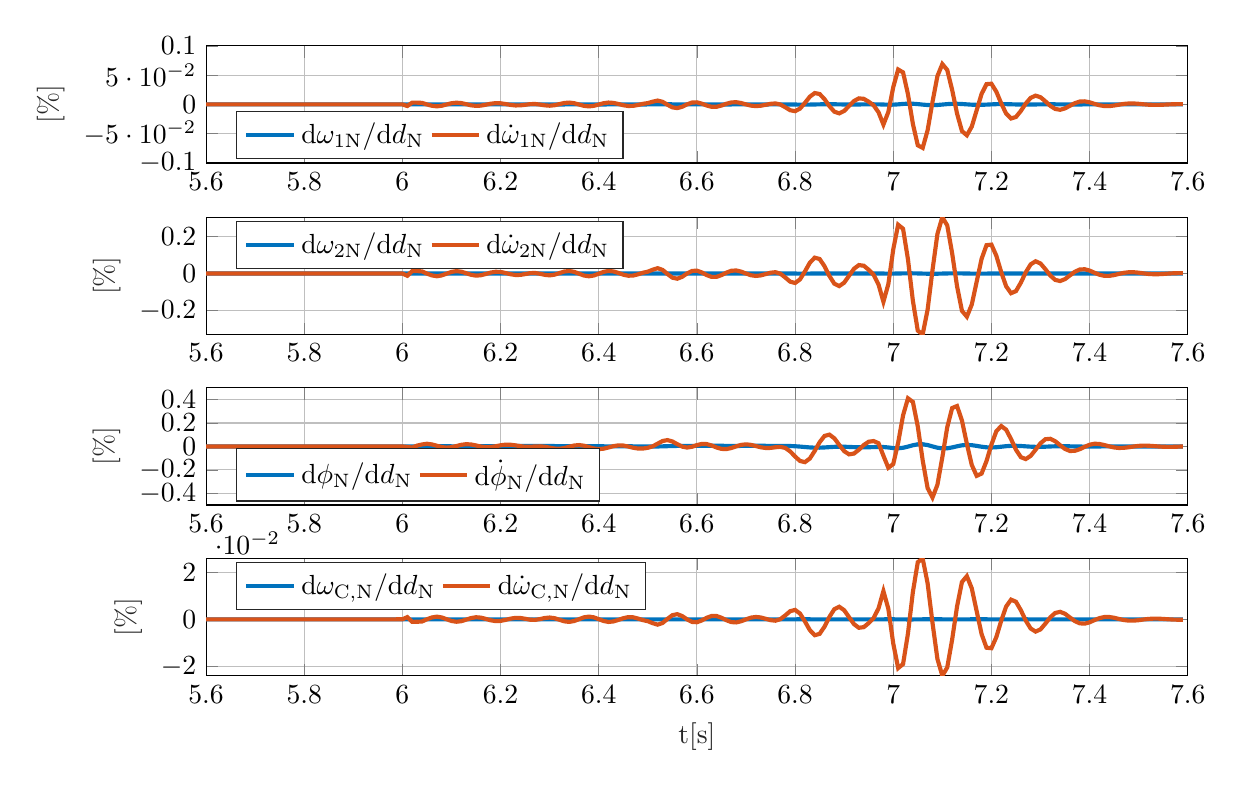
\begin{tikzpicture}

\begin{axis}[%
width=0.959\dwidth,
height=0.186\dheight,
at={(0\dwidth,0.814\dheight)},
scale only axis,
xmin=5.6,
xmax=7.6,
ymin=-0.1,
ymax=0.1,
ylabel style={font=\color{white!15!black}},
ylabel={[$\%$]},
axis background/.style={fill=white},
xmajorgrids,
ymajorgrids,
legend style={at={(0.03,0.03)}, anchor=south west, legend columns=2, legend cell align=left, align=left, draw=white!15!black}
]
\addplot [color=mycolor1, line width=1.5pt]
  table[row sep=crcr]{%
5.59	0\\
5.6	-4.30831767634006e-13\\
5.61	-9.82141155803885e-13\\
5.62	-1.45132344528616e-12\\
5.63	-2.01057116737164e-12\\
5.64	-2.45693386489609e-12\\
5.65	-2.97796650544282e-12\\
5.66	-3.39071158388908e-12\\
5.67	-3.89689463556598e-12\\
5.68	-4.3153423796627e-12\\
5.69	-4.83898141385465e-12\\
5.7	-5.27353213122402e-12\\
5.71	-4.58827469543543e-12\\
5.72	-1.83518348214983e-12\\
5.73	7.11539904284985e-13\\
5.74	-2.56802852090534e-13\\
5.75	-6.27338858011221e-12\\
5.76	-1.49069368140702e-11\\
5.77	-2.165603011614e-11\\
5.78	-2.22326704959997e-11\\
5.79	-1.59679600064292e-11\\
5.8	-5.81238545015398e-12\\
5.81	2.91326331542316e-12\\
5.82	5.90008818535518e-12\\
5.83	1.86040186864514e-12\\
5.84	-6.73042224831567e-12\\
5.85	-1.53016240452418e-11\\
5.86	-1.96501989842711e-11\\
5.87	-1.78065688709651e-11\\
5.88	-1.10524094100303e-11\\
5.89	-2.17846470106101e-12\\
5.9	5.22160685507638e-12\\
5.91	1.01408668320017e-11\\
5.92	7.2814729289131e-11\\
5.93	1.70499834569092e-09\\
5.94	2.44275902438312e-08\\
5.95	1.11205635648632e-07\\
5.96	2.57245268094344e-07\\
5.97	3.68497061346844e-07\\
5.98	3.17330271043247e-07\\
5.99	5.31802880659262e-08\\
6	-3.19585622998285e-07\\
6.01	-1.2959415665267e-05\\
6.02	-2.67691149595041e-05\\
6.03	2.17880803248147e-05\\
6.04	5.04164603662629e-05\\
6.05	6.80922126332615e-05\\
6.06	5.20418153974847e-05\\
6.07	1.89399958990366e-05\\
6.08	-1.55826620410975e-05\\
6.09	-3.04289153578281e-05\\
6.1	-1.95478134751785e-05\\
6.11	1.04615274404272e-05\\
6.12	4.17338630350636e-05\\
6.13	5.75921462770771e-05\\
6.14	5.01285468209688e-05\\
6.15	2.50491605811897e-05\\
6.16	-3.052808157494e-06\\
6.17	-1.88688717510645e-05\\
6.18	-1.48351905829751e-05\\
6.19	5.13813259497739e-06\\
6.2	2.96341626759476e-05\\
6.21	4.52358720322147e-05\\
6.22	4.41563808322684e-05\\
6.23	2.8466830571032e-05\\
6.24	7.51588737275339e-06\\
6.25	-7.02626024384875e-06\\
6.26	-7.67867568292319e-06\\
6.27	1.26765737493943e-07\\
6.28	3.4047038935846e-06\\
6.29	-7.56636213984137e-06\\
6.3	-3.07597257581592e-05\\
6.31	-5.30758248634155e-05\\
6.32	-5.86658803140156e-05\\
6.33	-4.08086358292052e-05\\
6.34	-7.20908784979998e-06\\
6.35	2.39903070259515e-05\\
6.36	3.5153712039654e-05\\
6.37	1.88993066948357e-05\\
6.38	-1.63103645169149e-05\\
6.39	-5.13642368758169e-05\\
6.4	-6.72457688288652e-05\\
6.41	-5.6398792398586e-05\\
6.42	-2.55419777170449e-05\\
6.43	8.27751098313268e-06\\
6.44	2.75918165747605e-05\\
6.45	2.34781048721751e-05\\
6.46	-1.35141185940008e-06\\
6.47	-3.26060904016496e-05\\
6.48	-5.34479052516628e-05\\
6.49	-5.34337496945309e-05\\
6.5	-3.39172239735319e-05\\
6.51	3.87956981737562e-06\\
6.52	7.12202681771509e-05\\
6.53	0.000137972632873364\\
6.54	0.000161613574276918\\
6.55	0.000126799853594793\\
6.56	5.7744432513692e-05\\
6.57	-4.78832003522571e-06\\
6.58	-2.7952714882798e-05\\
6.59	-7.55207541653974e-06\\
6.6	3.38368914021719e-05\\
6.61	6.37690573924369e-05\\
6.62	6.03098209633385e-05\\
6.63	2.38125105608474e-05\\
6.64	-2.5783207033256e-05\\
6.65	-6.19139958905386e-05\\
6.66	-6.68221069891359e-05\\
6.67	-4.00817382520885e-05\\
6.68	2.66640900720789e-06\\
6.69	3.94046617582281e-05\\
6.7	5.33244634444202e-05\\
6.71	4.04959162053505e-05\\
6.72	1.02239892806299e-05\\
6.73	-2.11766926736998e-05\\
6.74	-3.9072151754468e-05\\
6.75	-3.72374805127988e-05\\
6.76	-2.0090779300942e-05\\
6.77	-1.00142598343172e-05\\
6.78	-3.81877597053639e-05\\
6.79	-0.000125612740509086\\
6.8	-0.000255110632340129\\
6.81	-0.00036837939792308\\
6.82	-0.000398895297525212\\
6.83	-0.000307979944796254\\
6.84	-0.000114507201932795\\
6.85	0.000107424765535459\\
6.86	0.000266577314354131\\
6.87	0.000300745105658637\\
6.88	0.000206859341053337\\
6.89	3.96172438244971e-05\\
6.9	-0.000119164270300733\\
6.91	-0.000200886664279836\\
6.92	-0.000180649055044502\\
6.93	-8.3084081612616e-05\\
6.94	3.6017151293659e-05\\
6.95	0.000119911006960783\\
6.96	0.000136992458162182\\
6.97	8.25564503619923e-05\\
6.98	-0.000235867842339199\\
6.99	-0.000541900982840649\\
7	-0.000448218134451717\\
7.01	9.48953286433936e-05\\
7.02	0.000787725850237172\\
7.03	0.0012231625979619\\
7.04	0.0011309938552358\\
7.05	0.000508471212391878\\
7.06	-0.000354448284870544\\
7.07	-0.0010582889786163\\
7.08	-0.00129690976336356\\
7.09	-0.000975013560976583\\
7.1	-0.000274995167000601\\
7.11	0.000486747310051922\\
7.12	0.00097598239266593\\
7.13	0.00102719022437697\\
7.14	0.000657879438160034\\
7.15	6.59338384738917e-05\\
7.16	-0.000470774633826525\\
7.17	-0.000746249196295552\\
7.18	-0.000689508793064418\\
7.19	-0.000371212125992056\\
7.2	4.58263398431003e-05\\
7.21	0.000385574670531552\\
7.22	0.000518368219043633\\
7.23	0.000425980492310332\\
7.24	0.000187791939454705\\
7.25	-8.26381521762875e-05\\
7.26	-0.0002723732361666\\
7.27	-0.000320248083759635\\
7.28	-0.000239758377799904\\
7.29	-8.27066140114438e-05\\
7.3	7.98929492039389e-05\\
7.31	0.000184122513688753\\
7.32	0.000194459118269577\\
7.33	0.000132531824910331\\
7.34	3.1287410727672e-05\\
7.35	-6.38047870073148e-05\\
7.36	-0.000114865673980443\\
7.37	-0.000111714973952681\\
7.38	-6.91500764083011e-05\\
7.39	-9.15600581283641e-06\\
7.4	4.28752568580703e-05\\
7.41	6.94311147463029e-05\\
7.42	6.26772056643359e-05\\
7.43	3.6183059160036e-05\\
7.44	2.69154477283973e-06\\
7.45	-2.52018618994143e-05\\
7.46	-3.87512060652912e-05\\
7.47	-3.4517386049863e-05\\
7.48	-1.94829745099465e-05\\
7.49	-6.4472858473597e-07\\
7.5	1.47180428152034e-05\\
7.51	2.16138000257711e-05\\
7.52	1.85320021182538e-05\\
7.53	1.00427287157604e-05\\
7.54	1.11793719962074e-08\\
7.55	-7.78356324326664e-06\\
7.56	-1.09726232408441e-05\\
7.57	-9.55708890743882e-06\\
7.58	-5.26843792254145e-06\\
7.59	3.1916860888301e-08\\
};
\addlegendentry{d$\omega_{1\mathrm{N}}/$d$d_\mathrm{N}$}

\addplot [color=mycolor2, line width=1.5pt]
  table[row sep=crcr]{%
5.59	-4.98899172460086e-11\\
5.6	-3.25211340712767e-11\\
5.61	-5.42785142101515e-11\\
5.62	-3.51363707191503e-11\\
5.63	-5.39515631955255e-11\\
5.64	-3.24032393439167e-11\\
5.65	-5.04916387560489e-11\\
5.66	-2.98905317782809e-11\\
5.67	-4.98611666608069e-11\\
5.68	-3.09087507638327e-11\\
5.69	-5.15383302514616e-11\\
5.7	-3.20823309883498e-11\\
5.71	1.21949855075323e-10\\
5.72	2.97911110570443e-10\\
5.73	1.62883097257819e-10\\
5.74	-2.19984070496887e-10\\
5.75	-6.60125921308039e-10\\
5.76	-7.5989232469609e-10\\
5.77	-4.58302108284436e-10\\
5.78	1.74977700466346e-10\\
5.79	7.19689820490606e-10\\
5.8	9.35273571035191e-10\\
5.81	6.3935315266323e-10\\
5.82	6.62798139116329e-11\\
5.83	-5.34327807720652e-10\\
5.84	-7.93917604725937e-10\\
5.85	-6.60203016571779e-10\\
5.86	-1.71950634888627e-10\\
5.87	3.60894725122205e-10\\
5.88	7.47495509155084e-10\\
5.89	8.12793473475699e-10\\
5.9	6.52451280064071e-10\\
5.91	4.08360910682505e-10\\
5.92	2.30645109570623e-08\\
5.93	4.71587704325445e-07\\
5.94	4.19252372462251e-06\\
5.95	1.09697508773904e-05\\
5.96	1.30607544707775e-05\\
5.97	4.20791477213271e-06\\
5.98	-1.39752722483269e-05\\
5.99	-3.02861672169744e-05\\
6	-3.16074085469792e-05\\
6.01	-0.00272444404402052\\
6.02	0.00306660289606148\\
6.03	0.00297723383561637\\
6.04	0.00258891598577774\\
6.05	-9.64903967001968e-05\\
6.06	-0.00228381675086697\\
6.07	-0.00329760859237714\\
6.08	-0.00231586628536699\\
6.09	-0.000193116169226226\\
6.1	0.00199900894611586\\
6.11	0.00292426117668466\\
6.12	0.00224980616679111\\
6.13	0.000366967513705075\\
6.14	-0.00157327239561876\\
6.15	-0.00255427262400685\\
6.16	-0.00208376398605979\\
6.17	-0.000536244636968484\\
6.18	0.00118624110543633\\
6.19	0.002146718169662\\
6.2	0.00190964671664699\\
6.21	0.000671235564343844\\
6.22	-0.000828821250353229\\
6.23	-0.00176511348489549\\
6.24	-0.0016910513601129\\
6.25	-0.000720872133661512\\
6.26	0.000448766255104491\\
6.27	0.000712537837877697\\
6.28	-0.000269695315085232\\
6.29	-0.0016070292314795\\
6.3	-0.00222488237450772\\
6.31	-0.00139898085993134\\
6.32	0.00053699420556258\\
6.33	0.00244594257498005\\
6.34	0.00310250929379916\\
6.35	0.00203036038965083\\
6.36	-0.000241601553157289\\
6.37	-0.00246340823319312\\
6.38	-0.00335585757051968\\
6.39	-0.00242935462763715\\
6.4	-0.000200279960198517\\
6.41	0.00203467983304381\\
6.42	0.00316313747806166\\
6.43	0.00253199944439886\\
6.44	0.000726335546727614\\
6.45	-0.00140504277411816\\
6.46	-0.00268417700843464\\
6.47	-0.00248193002581887\\
6.48	-0.000970829815680307\\
6.49	0.000956185732577297\\
6.5	0.00225219259551452\\
6.51	0.00466707394169134\\
6.52	0.00650910021481602\\
6.53	0.00443002747734121\\
6.54	-0.000569050803672887\\
6.55	-0.00505173360522134\\
6.56	-0.0063300171990497\\
6.57	-0.00400291065871166\\
6.58	5.19457855735976e-05\\
6.59	0.00314206977372939\\
6.6	0.00354099565276627\\
6.61	0.00131594650448195\\
6.62	-0.00190645853347003\\
6.63	-0.00411392126371995\\
6.64	-0.00407459002697304\\
6.65	-0.0019223887778328\\
6.66	0.0010741640314381\\
6.67	0.00332029105531017\\
6.68	0.00375843175064164\\
6.69	0.0023582740533536\\
6.7	-1.87829208183695e-06\\
6.71	-0.00207872913511741\\
6.72	-0.00292280874489596\\
6.73	-0.0023010711700148\\
6.74	-0.00070546450501232\\
6.75	0.000973830531382013\\
6.76	0.00163414783924399\\
6.77	-0.000197332012594622\\
6.78	-0.00481318252723054\\
6.79	-0.0099388936850086\\
6.8	-0.0115620089857572\\
6.81	-0.00716302455518844\\
6.82	0.00244013003457478\\
6.83	0.0130948615212485\\
6.84	0.0193476314446542\\
6.85	0.0177576524550945\\
6.86	0.00889735968246694\\
6.87	-0.00301447589753206\\
6.88	-0.0124272585901705\\
6.89	-0.0153341407876014\\
6.9	-0.0111579285811837\\
6.91	-0.00264412044719487\\
6.92	0.00576964902160533\\
6.93	0.0103008165484387\\
6.94	0.00949909336310895\\
6.95	0.00458195102106744\\
6.96	-0.00155062345465285\\
6.97	-0.0133979389007247\\
6.98	-0.0344286849091058\\
6.99	-0.0129442203049414\\
7	0.0294080750200183\\
7.01	0.0595652226344242\\
7.02	0.0546553406988504\\
7.03	0.0173477552044194\\
7.04	-0.0332620246587181\\
7.05	-0.0697978337977169\\
7.06	-0.0742434269606503\\
7.07	-0.0442374571878472\\
7.08	0.00425439438677921\\
7.09	0.0482515351419329\\
7.1	0.068844138469317\\
7.11	0.0587875284833021\\
7.12	0.0247866017230693\\
7.13	-0.0155948028972907\\
7.14	-0.0455578823174211\\
7.15	-0.0527143262168949\\
7.16	-0.0378993314591196\\
7.17	-0.00995655140470502\\
7.18	0.0179059348922258\\
7.19	0.0345897367714203\\
7.2	0.035272480257382\\
7.21	0.0217671908270993\\
7.22	0.00172678198486632\\
7.23	-0.0155757095936112\\
7.24	-0.0240203644179055\\
7.25	-0.0214677247105953\\
7.26	-0.0111694673650278\\
7.27	0.00149771438286218\\
7.28	0.0111841535350316\\
7.29	0.0149596944482959\\
7.3	0.0122506197545902\\
7.31	0.00523937272104222\\
7.32	-0.00244468103537259\\
7.33	-0.00777587561185838\\
7.34	-0.00917288390788656\\
7.35	-0.0067903394218489\\
7.36	-0.00225403555859075\\
7.37	0.00213370274866475\\
7.38	0.00485962058494995\\
7.39	0.00525088810404354\\
7.4	0.00361846109969423\\
7.41	0.000944436328077961\\
7.42	-0.00145944279092249\\
7.43	-0.00279097917415653\\
7.44	-0.00287950549522102\\
7.45	-0.00191260698799216\\
7.46	-0.000446096563656461\\
7.47	0.000865920994425859\\
7.48	0.00158673653820018\\
7.49	0.00159121465351968\\
7.5	0.00101086651736129\\
7.51	0.000175377089979438\\
7.52	-0.000511584869468801\\
7.53	-0.000855771911937585\\
7.54	-0.000838596987113826\\
7.55	-0.00051482484109793\\
7.56	-8.75152070895476e-05\\
7.57	0.00026649597617993\\
7.58	0.000454162181832091\\
7.59	0.000442377709166627\\
};
\addlegendentry{d$\dot{\omega}_{1\mathrm{N}}/$d$d_\mathrm{N}$}

\end{axis}

\begin{axis}[%
width=0.959\dwidth,
height=0.186\dheight,
at={(0\dwidth,0.542\dheight)},
scale only axis,
xmin=5.6,
xmax=7.6,
ymin=-0.327126119151431,
ymax=0.303336157364176,
ylabel style={font=\color{white!15!black}},
ylabel={[$\%$]},
axis background/.style={fill=white},
xmajorgrids,
ymajorgrids,
legend style={at={(0.03,0.97)}, anchor=north west, legend columns=2, legend cell align=left, align=left, draw=white!15!black}
]
\addplot [color=mycolor1, line width=1.5pt]
  table[row sep=crcr]{%
5.59	0\\
5.6	-4.05003529267988e-13\\
5.61	-9.23231508307734e-13\\
5.62	-1.36429107796719e-12\\
5.63	-1.89000841233135e-12\\
5.64	-2.30958621113337e-12\\
5.65	-2.79935063210531e-12\\
5.66	-3.18731820747639e-12\\
5.67	-3.66311011591371e-12\\
5.68	-4.05645308687765e-12\\
5.69	-4.54867001668629e-12\\
5.7	-4.95712485710965e-12\\
5.71	-4.3130445805491e-12\\
5.72	-1.72524699265175e-12\\
5.73	6.68580910241625e-13\\
5.74	-2.41661627315677e-13\\
5.75	-5.8970621357139e-12\\
5.76	-1.40123206786574e-11\\
5.77	-2.03562663644601e-11\\
5.78	-2.08983060830011e-11\\
5.79	-1.50096762249082e-11\\
5.8	-5.46374978614659e-12\\
5.81	2.73805558915728e-12\\
5.82	5.54556279331524e-12\\
5.83	1.7483688237063e-12\\
5.84	-6.32675079702913e-12\\
5.85	-1.4383400440695e-11\\
5.86	-1.8470925798312e-11\\
5.87	-1.6737989674342e-11\\
5.88	-1.03893089948536e-11\\
5.89	-2.04807495262096e-12\\
5.9	4.90773625866457e-12\\
5.91	9.53166851841528e-12\\
5.92	6.8443067626691e-11\\
5.93	1.60264333553865e-09\\
5.94	2.29611513485726e-08\\
5.95	1.04529732370749e-07\\
5.96	2.41802305609447e-07\\
5.97	3.46375425132554e-07\\
5.98	2.98280282488919e-07\\
5.99	4.99877657542033e-08\\
6	-3.00400241788632e-07\\
6.01	-1.21814353143114e-05\\
6.02	-2.51621099419311e-05\\
6.03	2.04800970558283e-05\\
6.04	4.73898566212704e-05\\
6.05	6.40044971934259e-05\\
6.06	4.89176383295751e-05\\
6.07	1.78029890428787e-05\\
6.08	-1.46472026142815e-05\\
6.09	-2.86022049667065e-05\\
6.1	-1.83743178755681e-05\\
6.11	9.83350059081518e-06\\
6.12	3.92284936276739e-05\\
6.13	5.41347714720899e-05\\
6.14	4.71192272480317e-05\\
6.15	2.35454080783015e-05\\
6.16	-2.86954173594049e-06\\
6.17	-1.77361345340978e-05\\
6.18	-1.3944603536256e-05\\
6.19	4.82967989446194e-06\\
6.2	2.78551629244342e-05\\
6.21	4.25202696271506e-05\\
6.22	4.15055825049222e-05\\
6.23	2.67579082183092e-05\\
6.24	7.06469319163397e-06\\
6.25	-6.60445942516435e-06\\
6.26	-7.21770892894806e-06\\
6.27	1.19155796491361e-07\\
6.28	3.20031256567702e-06\\
6.29	-7.11213784093578e-06\\
6.3	-2.89131561595583e-05\\
6.31	-4.98895739447612e-05\\
6.32	-5.51440468802247e-05\\
6.33	-3.83588094824942e-05\\
6.34	-6.77631141548765e-06\\
6.35	2.25501196788869e-05\\
6.36	3.30433626520707e-05\\
6.37	1.77647428171867e-05\\
6.38	-1.53312194849436e-05\\
6.39	-4.82807358350454e-05\\
6.4	-6.32088668039681e-05\\
6.41	-5.3013056656396e-05\\
6.42	-2.40086401279074e-05\\
6.43	7.78059514215461e-06\\
6.44	2.59354232072587e-05\\
6.45	2.20686660935398e-05\\
6.46	-1.27028372998383e-06\\
6.47	-3.06486796615198e-05\\
6.48	-5.02393175441832e-05\\
6.49	-5.02260118049322e-05\\
6.5	-3.18811032230773e-05\\
6.51	3.64667136954438e-06\\
6.52	6.69447692409415e-05\\
6.53	0.000129689852329974\\
6.54	0.000151911579436969\\
6.55	0.000119187797966707\\
6.56	5.42779157857621e-05\\
6.57	-4.50086721129404e-06\\
6.58	-2.62746558771885e-05\\
6.59	-7.09870871664446e-06\\
6.6	3.1805593402078e-05\\
6.61	5.99408699709458e-05\\
6.62	5.668929861192e-05\\
6.63	2.23829967456338e-05\\
6.64	-2.4235388031729e-05\\
6.65	-5.81971713937226e-05\\
6.66	-6.28106384979545e-05\\
6.67	-3.7675549033168e-05\\
6.68	2.50633910931094e-06\\
6.69	3.70391190612668e-05\\
6.7	5.01232864523815e-05\\
6.71	3.80648632630836e-05\\
6.72	9.61022231286533e-06\\
6.73	-1.99054121832255e-05\\
6.74	-3.67265700898487e-05\\
6.75	-3.50020379328457e-05\\
6.76	-1.8884688579149e-05\\
6.77	-9.41308371606627e-06\\
6.78	-3.5895270886956e-05\\
6.79	-0.000118071950730522\\
6.8	-0.000239795818085508\\
6.81	-0.000346264826802921\\
6.82	-0.000374948794048706\\
6.83	-0.000289491277018449\\
6.84	-0.00010763310052762\\
6.85	0.000100975834912424\\
6.86	0.000250574129219983\\
6.87	0.000282690757813348\\
6.88	0.00019444114856228\\
6.89	3.72389380672504e-05\\
6.9	-0.000112010595509199\\
6.91	-0.000188827026267692\\
6.92	-0.000169804322297944\\
6.93	-7.80963746929659e-05\\
6.94	3.38549664789898e-05\\
6.95	0.000112712501608685\\
6.96	0.00012876851819619\\
6.97	7.76004158014616e-05\\
6.98	-0.000221708212248292\\
6.99	-0.000509369554493256\\
7	-0.000421310679999675\\
7.01	8.9198565974563e-05\\
7.02	0.000740437047748107\\
7.03	0.00114973363269022\\
7.04	0.00106309796895736\\
7.05	0.00047794663936344\\
7.06	-0.000333170027356589\\
7.07	-0.000994757718151963\\
7.08	-0.00121905360686635\\
7.09	-0.000916481494869271\\
7.1	-0.000258486643440558\\
7.11	0.000457526867510836\\
7.12	0.000917392162953098\\
7.13	0.000965525883277263\\
7.14	0.000618385582338199\\
7.15	6.1975693270581e-05\\
7.16	-0.00044251306678612\\
7.17	-0.000701450325330977\\
7.18	-0.000648116164891352\\
7.19	-0.000348927500630104\\
7.2	4.30752892917002e-05\\
7.21	0.000362427829504819\\
7.22	0.000487249508454281\\
7.23	0.000400408006780002\\
7.24	0.000176518402076788\\
7.25	-7.76772157032241e-05\\
7.26	-0.000256022112767669\\
7.27	-0.000301022934893343\\
7.28	-0.000225365191367538\\
7.29	-7.77415676682618e-05\\
7.3	7.50968096660132e-05\\
7.31	0.000173069258921623\\
7.32	0.000182785335941539\\
7.33	0.000124575665187456\\
7.34	2.94091611607556e-05\\
7.35	-5.99744565441658e-05\\
7.36	-0.00010797005356385\\
7.37	-0.000105008496534016\\
7.38	-6.49988572342287e-05\\
7.39	-8.60635394759002e-06\\
7.4	4.03013651147233e-05\\
7.41	6.52630202855956e-05\\
7.42	5.8914562243483e-05\\
7.43	3.40109137445898e-05\\
7.44	2.52996369291492e-06\\
7.45	-2.3688944464106e-05\\
7.46	-3.64248935283155e-05\\
7.47	-3.24452384347942e-05\\
7.48	-1.83133735076061e-05\\
7.49	-6.06026171705509e-07\\
7.5	1.38344864950135e-05\\
7.51	2.03162772308166e-05\\
7.52	1.74194859840656e-05\\
7.53	9.43984108284203e-06\\
7.54	1.05062389207755e-08\\
7.55	-7.31630197244438e-06\\
7.56	-1.03139161533206e-05\\
7.57	-8.98335925437063e-06\\
7.58	-4.95216480016493e-06\\
7.59	2.99988039650026e-08\\
};
\addlegendentry{d$\omega_{2\mathrm{N}}/$d$d_\mathrm{N}$}

\addplot [color=mycolor2, line width=1.5pt]
  table[row sep=crcr]{%
5.59	-2.19823363257795e-10\\
5.6	-1.43292024156739e-10\\
5.61	-2.39168058204528e-10\\
5.62	-1.54812445029881e-10\\
5.63	-2.37724499734465e-10\\
5.64	-1.42774811833676e-10\\
5.65	-2.22486200984853e-10\\
5.66	-1.31711647286073e-10\\
5.67	-2.19704187588456e-10\\
5.68	-1.36175838888446e-10\\
5.69	-2.27080333151836e-10\\
5.7	-1.41344857375996e-10\\
5.71	5.37320732384139e-10\\
5.72	1.31264205237236e-09\\
5.73	7.17691818643507e-10\\
5.74	-9.69278588343697e-10\\
5.75	-2.90860518627617e-09\\
5.76	-3.34819048030923e-09\\
5.77	-2.01932825543543e-09\\
5.78	7.70974998695937e-10\\
5.79	3.17104735409157e-09\\
5.8	4.1209287092497e-09\\
5.81	2.81708347476967e-09\\
5.82	2.92031962333878e-10\\
5.83	-2.35432428222806e-09\\
5.84	-3.49809579451684e-09\\
5.85	-2.90893453697864e-09\\
5.86	-7.57636981411544e-10\\
5.87	1.59013714730041e-09\\
5.88	3.29356544507792e-09\\
5.89	3.58126191761757e-09\\
5.9	2.87478106107014e-09\\
5.91	1.79928941917433e-09\\
5.92	1.01625202931355e-07\\
5.93	2.07787627808879e-06\\
5.94	1.84728005034876e-05\\
5.95	4.83341378474538e-05\\
5.96	5.75473694901049e-05\\
5.97	1.85406154469344e-05\\
5.98	-6.1576852819062e-05\\
5.99	-0.000133444760728205\\
6	-0.000139266320499388\\
6.01	-0.0120042520052118\\
6.02	0.0135118480575867\\
6.03	0.0131180764455706\\
6.04	0.0114070978927906\\
6.05	-0.000425149138449178\\
6.06	-0.0100627912954518\\
6.07	-0.0145296889632518\\
6.08	-0.0102040056799482\\
6.09	-0.000850894760256931\\
6.1	0.00880789135766455\\
6.11	0.012884672075035\\
6.12	0.0099129362734748\\
6.13	0.00161690621684761\\
6.14	-0.00693204118150148\\
6.15	-0.0112544547706529\\
6.16	-0.00918133300001954\\
6.17	-0.00236276306454215\\
6.18	0.00522673137655952\\
6.19	0.00945871725622453\\
6.2	0.00841414984382922\\
6.21	0.00295755050903856\\
6.22	-0.0036518933755888\\
6.23	-0.00777731777497329\\
6.24	-0.00745099049659928\\
6.25	-0.00317625563828463\\
6.26	0.00197732202631894\\
6.27	0.00313953365563837\\
6.28	-0.001188312358272\\
6.29	-0.00708077815609718\\
6.3	-0.00980311882864134\\
6.31	-0.00616409018564069\\
6.32	0.00236606576048301\\
6.33	0.0107771385963022\\
6.34	0.0136700562791832\\
6.35	0.00894602986333149\\
6.36	-0.00106452761814142\\
6.37	-0.0108540945400821\\
6.38	-0.0147863414770877\\
6.39	-0.010704049959904\\
6.4	-0.000882459347656749\\
6.41	0.00896506188826921\\
6.42	0.0139371918821679\\
6.43	0.0111563162672757\\
6.44	0.00320032814120808\\
6.45	-0.00619079976175083\\
6.46	-0.0118268302505892\\
6.47	-0.0109357039483433\\
6.48	-0.00427760143842111\\
6.49	0.00421307771866356\\
6.5	0.00992345118636321\\
6.51	0.0205637300006078\\
6.52	0.0286799354448959\\
6.53	0.019519272691509\\
6.54	-0.00250731126817115\\
6.55	-0.0222585901124827\\
6.56	-0.0278908725695515\\
6.57	-0.0176373408758298\\
6.58	0.000228879834043181\\
6.59	0.0138443648584205\\
6.6	0.0156020837566531\\
6.61	0.00579823010122658\\
6.62	-0.00840010229737922\\
6.63	-0.0181264679256902\\
6.64	-0.0179531694214912\\
6.65	-0.00847029300960673\\
6.66	0.00473290532672635\\
6.67	0.0146296308217702\\
6.68	0.0165601352606557\\
6.69	0.0103908597777616\\
6.7	-8.2759972673005e-06\\
6.71	-0.00915914879708469\\
6.72	-0.0128782724731368\\
6.73	-0.010138816492643\\
6.74	-0.00310836763834476\\
6.75	0.00429082297898705\\
6.76	0.00720026624113955\\
6.77	-0.00086947031012877\\
6.78	-0.0212075032815378\\
6.79	-0.0437920480362363\\
6.8	-0.0509437034891891\\
6.81	-0.0315612104673806\\
6.82	0.010751527793292\\
6.83	0.0576976495514165\\
6.84	0.0852481606569103\\
6.85	0.0782425080667899\\
6.86	0.0392029148272354\\
6.87	-0.0132821697759048\\
6.88	-0.0547561048932847\\
6.89	-0.0675642029432375\\
6.9	-0.0491632730863282\\
6.91	-0.0116503358730807\\
6.92	0.0254218180728924\\
6.93	0.0453867268730306\\
6.94	0.0418542310685185\\
6.95	0.0201886674285443\\
6.96	-0.00683224702509764\\
6.97	-0.0590330475928371\\
6.98	-0.151697228197366\\
6.99	-0.0570339049144644\\
7	0.129575773194193\\
7.01	0.262452056895471\\
7.02	0.240818483543204\\
7.03	0.0764364478894275\\
7.04	-0.146556772594738\\
7.05	-0.3075382620407\\
7.06	-0.327126119151431\\
7.07	-0.194915944527443\\
7.08	0.0187454106317653\\
7.09	0.21260248994764\\
7.1	0.303336157364176\\
7.11	0.259025436116251\\
7.12	0.109212965518383\\
7.13	-0.0687127138329183\\
7.14	-0.200733908028727\\
7.15	-0.232266123277892\\
7.16	-0.166989344729845\\
7.17	-0.0438698502276697\\
7.18	0.0788958596183297\\
7.19	0.152406843483951\\
7.2	0.15541509938057\\
7.21	0.0959090515025864\\
7.22	0.00760842423974823\\
7.23	-0.0686285862732163\\
7.24	-0.105836825080788\\
7.25	-0.0945895651518196\\
7.26	-0.049214114456861\\
7.27	0.0065991228277047\\
7.28	0.049278823616909\\
7.29	0.0659143440557459\\
7.3	0.0539778113912033\\
7.31	0.0230853522687082\\
7.32	-0.0107715800900199\\
7.33	-0.0342615113020105\\
7.34	-0.0404169101165413\\
7.35	-0.0299191116806509\\
7.36	-0.00993157151948145\\
7.37	0.00940136963187032\\
7.38	0.0214121153559561\\
7.39	0.0231360905320972\\
7.4	0.0159434065115447\\
7.41	0.00416130832636182\\
7.42	-0.00643049325526203\\
7.43	-0.0122974143739187\\
7.44	-0.0126874727674732\\
7.45	-0.00842719318137199\\
7.46	-0.00196555902132355\\
7.47	0.00381535963512165\\
7.48	0.00699136593106383\\
7.49	0.00701109708497969\\
7.5	0.00445400831214803\\
7.51	0.000772734088139325\\
7.52	-0.00225410894698848\\
7.53	-0.00377064146809142\\
7.54	-0.00369496653315354\\
7.55	-0.00226838468004014\\
7.56	-0.000385603294915023\\
7.57	0.00117421565822433\\
7.58	0.00200109717572607\\
7.59	0.00194917326857415\\
};
\addlegendentry{d$\dot{\omega}_{2\mathrm{N}}/$d$d_\mathrm{N}$}

\end{axis}

\begin{axis}[%
width=0.959\dwidth,
height=0.186\dheight,
at={(0\dwidth,0.271\dheight)},
scale only axis,
xmin=5.6,
xmax=7.6,
ymin=-0.5,
ymax=0.5,
ylabel style={font=\color{white!15!black}},
ylabel={[$\%$]},
axis background/.style={fill=white},
xmajorgrids,
ymajorgrids,
legend style={at={(0.03,0.03)}, anchor=south west, legend columns=2, legend cell align=left, align=left, draw=white!15!black}
]
\addplot [color=mycolor1, line width=1.5pt]
  table[row sep=crcr]{%
5.59	-1.7571785426454e-05\\
5.6	-1.75880567631243e-05\\
5.61	-1.76043326335801e-05\\
5.62	-1.76206133210849e-05\\
5.63	-1.76368987213157e-05\\
5.64	-1.76531888166438e-05\\
5.65	-1.76694833011856e-05\\
5.66	-1.76857821378237e-05\\
5.67	-1.77020851573085e-05\\
5.68	-1.77183925190561e-05\\
5.69	-1.77347041974616e-05\\
5.7	-1.77510203813149e-05\\
5.71	-1.77673346592354e-05\\
5.72	-1.77836293025331e-05\\
5.73	-1.77998969145635e-05\\
5.74	-1.78161609151703e-05\\
5.75	-1.78324655063774e-05\\
5.76	-1.78488455802864e-05\\
5.77	-1.78652980803258e-05\\
5.78	-1.78817775205067e-05\\
5.79	-1.78982187262815e-05\\
5.8	-1.79145740605262e-05\\
5.81	-1.79308388962907e-05\\
5.82	-1.79470555821492e-05\\
5.83	-1.79632878642895e-05\\
5.84	-1.79795891298205e-05\\
5.85	-1.79959739180517e-05\\
5.86	-1.80124155380852e-05\\
5.87	-1.80288595220202e-05\\
5.88	-1.8045254640643e-05\\
5.89	-1.80615702715322e-05\\
5.9	-1.80778105458207e-05\\
5.91	-1.80939954799202e-05\\
5.92	-1.81100498676361e-05\\
5.93	-1.81211561167621e-05\\
5.94	-1.80454627085444e-05\\
5.95	-1.74813969647824e-05\\
5.96	-1.57765618084109e-05\\
5.97	-1.27481980715381e-05\\
5.98	-9.35050118526162e-06\\
5.99	-7.4708067379704e-06\\
6	-8.90745923033753e-06\\
6.01	-4.59330691756846e-05\\
6.02	-0.000296287362250685\\
6.03	-0.000314020730011289\\
6.04	3.07453194493806e-05\\
6.05	0.000619922103738984\\
6.06	0.00120863693439304\\
6.07	0.0015547067360528\\
6.08	0.00156187245829533\\
6.09	0.00132432521428081\\
6.1	0.00106712515979891\\
6.11	0.00101530672649506\\
6.12	0.00126822459519299\\
6.13	0.00175573268225603\\
6.14	0.00228416159602165\\
6.15	0.00264956264113954\\
6.16	0.00274992017817524\\
6.17	0.00263227471462845\\
6.18	0.00245850590391019\\
6.19	0.00240632023506295\\
6.2	0.0025727267533162\\
6.21	0.00293818681721887\\
6.22	0.00337511956815477\\
6.23	0.00372659910374524\\
6.24	0.00389641840899261\\
6.25	0.00388973664542247\\
6.26	0.00380970056806261\\
6.27	0.00377179352027374\\
6.28	0.00379581752206061\\
6.29	0.0037845271449667\\
6.3	0.00360862506627468\\
6.31	0.00320543023783025\\
6.32	0.00265827995074199\\
6.33	0.00216907495563362\\
6.34	0.00193517421494992\\
6.35	0.00202306468865094\\
6.36	0.002321988455186\\
6.37	0.00259942446558048\\
6.38	0.00262016794332361\\
6.39	0.00229195955347078\\
6.4	0.00170924446911483\\
6.41	0.00111349840963506\\
6.42	0.000719783916724749\\
6.43	0.000663089588006176\\
6.44	0.000846385480604075\\
6.45	0.00110757930790725\\
6.46	0.00122448823154071\\
6.47	0.00106284562153678\\
6.48	0.00064116324473768\\
6.49	0.000116861952352376\\
6.5	-0.000308905639251122\\
6.51	-0.000472002610148109\\
6.52	-0.000131299871009687\\
6.53	0.000877061607290799\\
6.54	0.0023400129107988\\
6.55	0.00374128839318238\\
6.56	0.00462704816211299\\
6.57	0.00485819615376562\\
6.58	0.00466538650565402\\
6.59	0.00446807156019049\\
6.6	0.00458676413302569\\
6.61	0.00506971479912994\\
6.62	0.00568734406751065\\
6.63	0.00610622143083818\\
6.64	0.00609649303205964\\
6.65	0.00566085707108913\\
6.66	0.00502291194134529\\
6.67	0.00449496899353623\\
6.68	0.00431348627384486\\
6.69	0.00452548175002075\\
6.7	0.00498650389442822\\
6.71	0.00545013967103359\\
6.72	0.00569807884105298\\
6.73	0.00564042266929001\\
6.74	0.00534019221664141\\
6.75	0.00496545296609172\\
6.76	0.00470056528271591\\
6.77	0.00458013684306464\\
6.78	0.00438521030982424\\
6.79	0.00363469652250587\\
6.8	0.00180836352458573\\
6.81	-0.00119387117713212\\
6.82	-0.00491090562320171\\
6.83	-0.00835901445444882\\
6.84	-0.0104198424473884\\
6.85	-0.0104392322260772\\
6.86	-0.00858557895212908\\
6.87	-0.00578695928789343\\
6.88	-0.00329344672625304\\
6.89	-0.00209869241585206\\
6.9	-0.00251196292806306\\
6.91	-0.00410688759931998\\
6.92	-0.00599227090371682\\
6.93	-0.0072834862385868\\
6.94	-0.00749857822468321\\
6.95	-0.00671410162251095\\
6.96	-0.00544004260030165\\
6.97	-0.00432571816303428\\
6.98	-0.00487814823483425\\
6.99	-0.00877909241540059\\
7	-0.0138337537898627\\
7.01	-0.0157032705339313\\
7.02	-0.0112523154910139\\
7.03	-0.00135981319151633\\
7.04	0.0102620195895472\\
7.05	0.0182721606874711\\
7.06	0.0190454266507946\\
7.07	0.0119777659318817\\
7.08	0.000377159663326758\\
7.09	-0.0107226648672958\\
7.1	-0.0168082255703958\\
7.11	-0.0157223183088927\\
7.12	-0.0084084686058912\\
7.13	0.00136941475391727\\
7.14	0.00962584349138544\\
7.15	0.0129515003808737\\
7.16	0.0108214695269149\\
7.17	0.00476941252856272\\
7.18	-0.00225515339909659\\
7.19	-0.00737784322276277\\
7.2	-0.00892631628127126\\
7.21	-0.00676105859604274\\
7.22	-0.00229011954205376\\
7.23	0.00230848111750164\\
7.24	0.00526992769899013\\
7.25	0.00565872076919302\\
7.26	0.00384289485368346\\
7.27	0.000898452763397902\\
7.28	-0.00182188639199548\\
7.29	-0.00339296755628963\\
7.3	-0.00338961353669463\\
7.31	-0.00208442800754584\\
7.32	-0.000219174228860659\\
7.33	0.00137230481624511\\
7.34	0.00215980133498243\\
7.35	0.00198409715605352\\
7.36	0.00107935878076145\\
7.37	-3.14686713460342e-05\\
7.38	-0.000906994934249483\\
7.39	-0.00128054793015747\\
7.4	-0.00111220739167186\\
7.41	-0.000564621319643089\\
7.42	7.23910917262101e-05\\
7.43	0.000534419037409309\\
7.44	0.000717664900009621\\
7.45	0.000608077072200597\\
7.46	0.000302545912077645\\
7.47	-5.2011520371128e-05\\
7.48	-0.000309666536748744\\
7.49	-0.000404754373723377\\
7.5	-0.000333511244508927\\
7.51	-0.000154271752876454\\
7.52	3.79143462506807e-05\\
7.53	0.000169985207528824\\
7.54	0.000217106973652519\\
7.55	0.000173580613423922\\
7.56	7.92274042775023e-05\\
7.57	-2.02907088013351e-05\\
7.58	-9.16937374850691e-05\\
7.59	-0.000116437048036679\\
};
\addlegendentry{d$\phi_\mathrm{N}/$d$d_\mathrm{N}$}

\addplot [color=mycolor2, line width=1.5pt]
  table[row sep=crcr]{%
5.59	-5.76432268004859e-07\\
5.6	-5.76573241496256e-07\\
5.61	-5.76754667197868e-07\\
5.62	-5.7690851693505e-07\\
5.63	-5.77092612440046e-07\\
5.64	-5.77238780750554e-07\\
5.65	-5.7741002421832e-07\\
5.66	-5.77544892711724e-07\\
5.67	-5.77711138408851e-07\\
5.68	-5.77847921993487e-07\\
5.69	-5.78020031063407e-07\\
5.7	-5.78162208529048e-07\\
5.71	-5.77928315030431e-07\\
5.72	-5.76999946779381e-07\\
5.73	-5.76140913966483e-07\\
5.74	-5.76462441632477e-07\\
5.75	-5.78479389557194e-07\\
5.76	-5.81375177018543e-07\\
5.77	-5.83637995959356e-07\\
5.78	-5.83827749586058e-07\\
5.79	-5.81719845369803e-07\\
5.8	-5.78305267201196e-07\\
5.81	-5.7537104237531e-07\\
5.82	-5.74364268385862e-07\\
5.83	-5.75717360800425e-07\\
5.84	-5.78598900429234e-07\\
5.85	-5.81473756404381e-07\\
5.86	-5.82930374719923e-07\\
5.87	-5.82307322975127e-07\\
5.88	-5.80035103017288e-07\\
5.89	-5.77051021023628e-07\\
5.9	-5.74562033922336e-07\\
5.91	-5.72906293168893e-07\\
5.92	-5.51853604758115e-07\\
5.93	-3.68062642712023e-09\\
5.94	7.62769092078261e-06\\
5.95	3.67718094056963e-05\\
5.96	8.58179661689553e-05\\
5.97	0.000123179142174964\\
5.98	0.000105991086034042\\
5.99	1.72734414722352e-05\\
6	-0.000107919823615411\\
6.01	-0.00435301303450364\\
6.02	-0.00899079073218774\\
6.03	0.00731733223710111\\
6.04	0.0169319179585176\\
6.05	0.0228677726306885\\
6.06	0.0174765820354619\\
6.07	0.00635886252131942\\
6.08	-0.00523569959474132\\
6.09	-0.0102216186989489\\
6.1	-0.00656689467288171\\
6.11	0.00351190275068149\\
6.12	0.0140145654586557\\
6.13	0.0193401212261019\\
6.14	0.0168328984088633\\
6.15	0.00840952105794134\\
6.16	-0.00102872585724078\\
6.17	-0.00634048176774749\\
6.18	-0.00498557276615581\\
6.19	0.00172259457454209\\
6.2	0.00994950160087416\\
6.21	0.0151890126983559\\
6.22	0.0148260096620335\\
6.23	0.00955625608475787\\
6.24	0.00251963456970189\\
6.25	-0.00236438638137906\\
6.26	-0.00258341538955999\\
6.27	3.8112579721272e-05\\
6.28	0.00113899800598355\\
6.29	-0.00254565791489096\\
6.3	-0.010335043652048\\
6.31	-0.01782955975724\\
6.32	-0.0197064251025944\\
6.33	-0.0137084931039746\\
6.34	-0.00242372022079054\\
6.35	0.00805461618240812\\
6.36	0.0118035742325619\\
6.37	0.00634418685395043\\
6.38	-0.0054811245396586\\
6.39	-0.0172537449739333\\
6.4	-0.0225870010687985\\
6.41	-0.0189433802361569\\
6.42	-0.00857959697209096\\
6.43	0.00277885732561741\\
6.44	0.00926544312125801\\
6.45	0.00788356529845761\\
6.46	-0.000455637024948669\\
6.47	-0.0109524601147339\\
6.48	-0.0179518133960066\\
6.49	-0.0179465081164797\\
6.5	-0.011391366984636\\
6.51	0.0013029902402283\\
6.52	0.0239192421513281\\
6.53	0.0463371983394456\\
6.54	0.0542755537802934\\
6.55	0.0425817710325466\\
6.56	0.0193883360915568\\
6.57	-0.00161374806617524\\
6.58	-0.00939338415361796\\
6.59	-0.00254154548860111\\
6.6	0.011358963749039\\
6.61	0.0214112823322669\\
6.62	0.0202488392442457\\
6.63	0.00799065268416313\\
6.64	-0.00866622777752948\\
6.65	-0.0208004152940431\\
6.66	-0.0224481434602065\\
6.67	-0.0134667348086143\\
6.68	0.000890576547662198\\
6.69	0.0132290281676833\\
6.7	0.0179035598968409\\
6.71	0.0135945620673917\\
6.72	0.0034273719440401\\
6.73	-0.00711859150892594\\
6.74	-0.0131285220739204\\
6.75	-0.0125119404183316\\
6.76	-0.00675287606213829\\
6.77	-0.00336851015924597\\
6.78	-0.0128304692231835\\
6.79	-0.0421916594240343\\
6.8	-0.0856820477962898\\
6.81	-0.123720584726165\\
6.82	-0.133965526587699\\
6.83	-0.103427642584804\\
6.84	-0.0384469685667047\\
6.85	0.0360896743019511\\
6.86	0.0895396459336668\\
6.87	0.101012047842801\\
6.88	0.0694775374067306\\
6.89	0.0133074217413431\\
6.9	-0.0400194731127613\\
6.91	-0.067464539588094\\
6.92	-0.0606656734241631\\
6.93	-0.0278967709350538\\
6.94	0.0121040182942882\\
6.95	0.0402792258056443\\
6.96	0.0460147333389979\\
6.97	0.0277310208791068\\
6.98	-0.0792123166318625\\
6.99	-0.181990487766399\\
7	-0.150521414427029\\
7.01	0.0318871263472319\\
7.02	0.264571951237853\\
7.03	0.41080439006633\\
7.04	0.379836835438558\\
7.05	0.170751905352164\\
7.06	-0.119063450320839\\
7.07	-0.355443285778063\\
7.08	-0.435572556806876\\
7.09	-0.327450765540577\\
7.1	-0.0923406528665392\\
7.11	0.163492065990399\\
7.12	0.327795580971845\\
7.13	0.344983479819266\\
7.14	0.220940349370802\\
7.15	0.022129798056166\\
7.16	-0.158123346476053\\
7.17	-0.250635978426162\\
7.18	-0.231572010396935\\
7.19	-0.124665486091299\\
7.2	0.015399997375683\\
7.21	0.129503347692487\\
7.22	0.174097742943886\\
7.23	0.143064080748868\\
7.24	0.0630644517961338\\
7.25	-0.0277608573170979\\
7.26	-0.0914821045493008\\
7.27	-0.107557885264612\\
7.28	-0.0805222206717864\\
7.29	-0.0277741521457877\\
7.3	0.0268354764957024\\
7.31	0.0618399404595909\\
7.32	0.0653095237438645\\
7.33	0.0445093173702418\\
7.34	0.0105051810744138\\
7.35	-0.0214316777066541\\
7.36	-0.038579683458917\\
7.37	-0.0375203162630178\\
7.38	-0.0232238054867569\\
7.39	-0.00307418544097301\\
7.4	0.0144005150316119\\
7.41	0.0233188036047526\\
7.42	0.0210497939554089\\
7.43	0.0121511445255985\\
7.44	0.000902704882430644\\
7.45	-0.00846527539063476\\
7.46	-0.0130155407291645\\
7.47	-0.0115932154168339\\
7.48	-0.00654357800562998\\
7.49	-0.000216584777088219\\
7.5	0.00494297877750603\\
7.51	0.00725874945398466\\
7.52	0.00622350929722685\\
7.53	0.00337221436630361\\
7.54	3.03245066119838e-06\\
7.55	-0.00261481218870832\\
7.56	-0.00368576726171831\\
7.57	-0.00321024760917701\\
7.58	-0.00176981205924419\\
7.59	1.03572883532774e-05\\
};
\addlegendentry{d$\dot{\phi}_\mathrm{N}/$d$d_\mathrm{N}$}

\end{axis}

\begin{axis}[%
width=0.959\dwidth,
height=0.186\dheight,
at={(0\dwidth,0\dheight)},
scale only axis,
xmin=5.6,
xmax=7.6,
xlabel style={font=\color{white!15!black}},
xlabel={t[s]},
ymin=-0.0239121713006459,
ymax=0.0257692172916418,
ylabel style={font=\color{white!15!black}},
ylabel={[$\%$]},
axis background/.style={fill=white},
xmajorgrids,
ymajorgrids,
legend style={at={(0.03,0.97)}, anchor=north west, legend columns=2, legend cell align=left, align=left, draw=white!15!black}
]
\addplot [color=mycolor1, line width=1.5pt]
  table[row sep=crcr]{%
5.59	0\\
5.6	2.65224472006632e-15\\
5.61	9.05649238129227e-15\\
5.62	1.28871900836903e-14\\
5.63	1.95224053568151e-14\\
5.64	2.26223410908329e-14\\
5.65	2.80459805717028e-14\\
5.66	3.00802360660356e-14\\
5.67	3.50242362572319e-14\\
5.68	3.72210031101737e-14\\
5.69	4.26952124153148e-14\\
5.7	4.5377701642304e-14\\
5.71	1.31034959845666e-14\\
5.72	-8.36797133757089e-14\\
5.73	-1.7393395570579e-13\\
5.74	-1.54408657229899e-13\\
5.75	2.26388136440256e-14\\
5.76	2.81185840811048e-13\\
5.77	4.80678190687374e-13\\
5.78	4.87352721547641e-13\\
5.79	2.80514405868343e-13\\
5.8	-4.75621234862222e-14\\
5.81	-3.30712496165712e-13\\
5.82	-4.34513505526647e-13\\
5.83	-3.18943544310999e-13\\
5.84	-6.14583316453896e-14\\
5.85	1.95169604145075e-13\\
5.86	3.19776060932152e-13\\
5.87	2.51021138630773e-13\\
5.88	2.90785799295548e-14\\
5.89	-2.5881608000989e-13\\
5.9	-5.00457921591635e-13\\
5.91	-6.64463843888261e-13\\
5.92	-2.63153836837818e-12\\
5.93	-5.35938650005658e-11\\
5.94	-7.62873210016461e-10\\
5.95	-3.47091342960354e-09\\
5.96	-8.02607736403345e-09\\
5.97	-1.14910060725408e-08\\
5.98	-9.88310830930468e-09\\
5.99	-1.62906545482565e-09\\
6	1.0006756601562e-08\\
6.01	4.04591304305143e-07\\
6.02	8.35069756293666e-07\\
6.03	-6.81243531472704e-07\\
6.04	-1.57417079634655e-06\\
6.05	-2.1243580447213e-06\\
6.06	-1.62140490814615e-06\\
6.07	-5.86725771568519e-07\\
6.08	4.91306130802587e-07\\
6.09	9.5418421801748e-07\\
6.1	6.1363388078647e-07\\
6.11	-3.23604607377899e-07\\
6.12	-1.29936810964148e-06\\
6.13	-1.79310472793241e-06\\
6.14	-1.55846335915768e-06\\
6.15	-7.74236388370282e-07\\
6.16	1.03578235468917e-07\\
6.17	5.97094586749892e-07\\
6.18	4.70608545232315e-07\\
6.19	-1.53247602758902e-07\\
6.2	-9.17673600471556e-07\\
6.21	-1.40376429575284e-06\\
6.22	-1.36874838492567e-06\\
6.23	-8.77772489997214e-07\\
6.24	-2.23050533485401e-07\\
6.25	2.3101639662401e-07\\
6.26	2.51137387229461e-07\\
6.27	7.2780673928017e-09\\
6.28	-9.50172259018714e-08\\
6.29	2.47524441866326e-07\\
6.3	9.71226224344794e-07\\
6.31	1.66684821675312e-06\\
6.32	1.83974374736703e-06\\
6.33	1.28064308336926e-06\\
6.34	2.30741212068372e-07\\
6.35	-7.43239380333994e-07\\
6.36	-1.09093221113028e-06\\
6.37	-5.82534068334423e-07\\
6.38	5.16989418405002e-07\\
6.39	1.61059136804691e-06\\
6.4	2.1047420488927e-06\\
6.41	1.76422208665777e-06\\
6.42	7.99482489963408e-07\\
6.43	-2.56748173061862e-07\\
6.44	-8.59307966940293e-07\\
6.45	-7.30061768884128e-07\\
6.46	4.56239605009249e-08\\
6.47	1.02109803032601e-06\\
6.48	1.67062783771142e-06\\
6.49	1.66859218880063e-06\\
6.5	1.05787008817347e-06\\
6.51	-1.2287805108914e-07\\
6.52	-2.22464112398083e-06\\
6.53	-4.306003324009e-06\\
6.54	-5.03977492647602e-06\\
6.55	-3.94841456463017e-06\\
6.56	-1.78938425333014e-06\\
6.57	1.63973027187778e-07\\
6.58	8.86711208096599e-07\\
6.59	2.49061590667807e-07\\
6.6	-1.04301254243477e-06\\
6.61	-1.97622353716744e-06\\
6.62	-1.86633532281947e-06\\
6.63	-7.25397753130303e-07\\
6.64	8.2324666217201e-07\\
6.65	1.95013224913297e-06\\
6.66	2.10143311706972e-06\\
6.67	1.26480633965373e-06\\
6.68	-7.06254542146845e-08\\
6.69	-1.21718898420543e-06\\
6.7	-1.65045702636442e-06\\
6.71	-1.2484663451593e-06\\
6.72	-3.02443427933132e-07\\
6.73	6.77892234393757e-07\\
6.74	1.23576886966567e-06\\
6.75	1.17731970814434e-06\\
6.76	6.41069267714001e-07\\
6.77	3.26036612068927e-07\\
6.78	1.20518276278714e-06\\
6.79	3.93283471339079e-06\\
6.8	7.97097968416874e-06\\
6.81	1.1498757118077e-05\\
6.82	1.24402899195112e-05\\
6.83	9.59080646441665e-06\\
6.84	3.54308844800182e-06\\
6.85	-3.38705386733007e-06\\
6.86	-8.35109489335095e-06\\
6.87	-9.40943674664513e-06\\
6.88	-6.47008124518184e-06\\
6.89	-1.24406230625965e-06\\
6.9	3.71283592898992e-06\\
6.91	6.25984424937633e-06\\
6.92	5.62213304323357e-06\\
6.93	2.57160010768919e-06\\
6.94	-1.14812852387656e-06\\
6.95	-3.76539569348513e-06\\
6.96	-4.29485915113066e-06\\
6.97	-2.59159021780997e-06\\
6.98	7.34993644168039e-06\\
6.99	1.68942552416704e-05\\
7	1.39533906897029e-05\\
7.01	-3.0117322083612e-06\\
7.02	-2.46325399055794e-05\\
7.03	-3.8199177401754e-05\\
7.04	-3.52853535343476e-05\\
7.05	-1.58216739616765e-05\\
7.06	1.11264295802666e-05\\
7.07	3.30829630281817e-05\\
7.08	4.04984648798458e-05\\
7.09	3.04126640853119e-05\\
7.1	8.53497346745482e-06\\
7.11	-1.52480258440987e-05\\
7.12	-3.05024395919243e-05\\
7.13	-3.20713046514468e-05\\
7.14	-2.05136428440549e-05\\
7.15	-2.01914619659031e-06\\
7.16	1.47336608144394e-05\\
7.17	2.33170015047731e-05\\
7.18	2.15235101447944e-05\\
7.19	1.15684730917669e-05\\
7.2	-1.45885333538173e-06\\
7.21	-1.20612178157701e-05\\
7.22	-1.61940295859005e-05\\
7.23	-1.32948791991856e-05\\
7.24	-5.84798168601666e-06\\
7.25	2.59773518571847e-06\\
7.26	8.51682334297677e-06\\
7.27	1.00026527926384e-05\\
7.28	7.48083266645498e-06\\
7.29	2.57182801719596e-06\\
7.3	-2.50553301466465e-06\\
7.31	-5.75618139816463e-06\\
7.32	-6.07316664988675e-06\\
7.33	-4.13447107116158e-06\\
7.34	-9.70544644100712e-07\\
7.35	1.99828099918629e-06\\
7.36	3.58990983283006e-06\\
7.37	3.48807386918075e-06\\
7.38	2.15621145765394e-06\\
7.39	2.8166172161672e-07\\
7.4	-1.34255463442781e-06\\
7.41	-2.17009011770141e-06\\
7.42	-1.95720827308825e-06\\
7.43	-1.12845700168271e-06\\
7.44	-8.20726612032038e-08\\
7.45	7.88592184591962e-07\\
7.46	1.21073498707945e-06\\
7.47	1.07742396560956e-06\\
7.48	6.07152963682619e-07\\
7.49	1.86094054655078e-08\\
7.5	-4.60889445699078e-07\\
7.51	-6.75658368475672e-07\\
7.52	-5.78825268212403e-07\\
7.53	-3.13324475990329e-07\\
7.54	7.03629131500275e-11\\
7.55	2.43335038068535e-07\\
7.56	3.42622726861097e-07\\
7.57	2.98110082578466e-07\\
7.58	1.63968694957624e-07\\
7.59	-1.61845392386481e-09\\
};
\addlegendentry{d$\omega_{\mathrm{C,N}}/$d$d_\mathrm{N}$}

\addplot [color=mycolor2, line width=1.5pt]
  table[row sep=crcr]{%
5.59	6.90974614490037e-12\\
5.6	8.7237201716704e-13\\
5.61	8.41792207215707e-12\\
5.62	1.76256292843012e-12\\
5.63	8.28499680055005e-12\\
5.64	7.95953386229057e-13\\
5.65	7.06880778729951e-12\\
5.66	-9.13105631002499e-14\\
5.67	6.83392953562779e-12\\
5.68	2.45096496442047e-13\\
5.69	7.39988184487483e-12\\
5.7	6.37534753034844e-13\\
5.71	-5.28232347069743e-11\\
5.72	-1.138418924524e-10\\
5.73	-6.68832413670748e-11\\
5.74	6.60372505845657e-11\\
5.75	2.18709020104485e-10\\
5.76	2.53122265271759e-10\\
5.77	1.48223512834242e-10\\
5.78	-7.16776649799591e-11\\
5.79	-2.60641351486955e-10\\
5.8	-3.35217847459427e-10\\
5.81	-2.32225977216679e-10\\
5.82	-3.31531774601006e-11\\
5.83	1.7528779536645e-10\\
5.84	2.65195992458394e-10\\
5.85	2.18539379693573e-10\\
5.86	4.88932249235603e-11\\
5.87	-1.36068611134312e-10\\
5.88	-2.70119069653061e-10\\
5.89	-2.92545801176562e-10\\
5.9	-2.36666357782767e-10\\
5.91	-1.5177185458236e-10\\
5.92	-8.016867436456e-09\\
5.93	-1.63711366734824e-07\\
5.94	-1.45509874282079e-06\\
5.95	-3.80596651424337e-06\\
5.96	-4.52804271605836e-06\\
5.97	-1.45108053647156e-06\\
5.98	4.86119437211271e-06\\
5.99	1.05175551730089e-05\\
6	1.09661583258373e-05\\
6.01	0.00094564398240162\\
6.02	-0.00106553436211984\\
6.03	-0.00103317683598157\\
6.04	-0.000897561011156625\\
6.05	3.53641051114837e-05\\
6.06	0.000794420770894964\\
6.07	0.00114552943766395\\
6.08	0.000803698093599538\\
6.09	6.62179982431661e-05\\
6.1	-0.000694646237236128\\
6.11	-0.00101509527779501\\
6.12	-0.000780049939410489\\
6.13	-0.000125845244344535\\
6.14	0.000547650799654822\\
6.15	0.000887590508648596\\
6.16	0.000723445791206488\\
6.17	0.000185672581038985\\
6.18	-0.000412308011015158\\
6.19	-0.00074526128407826\\
6.2	-0.000662270359080052\\
6.21	-0.000231833118846822\\
6.22	0.000288995122584273\\
6.23	0.000613667452434704\\
6.24	0.000587373716091389\\
6.25	0.000250101569687927\\
6.26	-0.000156045065677816\\
6.27	-0.000247418063184934\\
6.28	9.37291647588242e-05\\
6.29	0.000557783421539369\\
6.3	0.00077167802206782\\
6.31	0.000484287954872113\\
6.32	-0.000188086303107488\\
6.33	-0.000850428335838972\\
6.34	-0.00107747604417775\\
6.35	-0.000704335478287678\\
6.36	8.4856936511476e-05\\
6.37	0.000855875556460177\\
6.38	0.00116478243225956\\
6.39	0.000842106524795845\\
6.4	6.76751301733826e-05\\
6.41	-0.000708059280597692\\
6.42	-0.00109903311983169\\
6.43	-0.000878947918285432\\
6.44	-0.000251439268999137\\
6.45	0.00048851597280339\\
6.46	0.000931975333782357\\
6.47	0.000860882662321957\\
6.48	0.000335611543821802\\
6.49	-0.000333496885310362\\
6.5	-0.000782961076012982\\
6.51	-0.00162041978655102\\
6.52	-0.00225814764753838\\
6.53	-0.00153438526367936\\
6.54	0.000202079272460843\\
6.55	0.0017576117297798\\
6.56	0.00219954131232844\\
6.57	0.00138976820773105\\
6.58	-1.88278206420126e-05\\
6.59	-0.00109123035837232\\
6.6	-0.0012285947838794\\
6.61	-0.000455166752742223\\
6.62	0.000663638194626766\\
6.63	0.00142910800074233\\
6.64	0.00141406798609352\\
6.65	0.000665760891399719\\
6.66	-0.000374855570332897\\
6.67	-0.00115402173227192\\
6.68	-0.00130496188244214\\
6.69	-0.000817765550111837\\
6.7	2.12827407128542e-06\\
6.71	0.000722905446785699\\
6.72	0.00101514560093355\\
6.73	0.000798385007900162\\
6.74	0.000243849604391242\\
6.75	-0.00033919304982928\\
6.76	-0.000567992437745593\\
6.77	6.82268670835842e-05\\
6.78	0.0016701826329184\\
6.79	0.00344751954649822\\
6.8	0.00400748985934026\\
6.81	0.00247688711409389\\
6.82	-0.000858422337710288\\
6.83	-0.00455546984752348\\
6.84	-0.00672117502449781\\
6.85	-0.00616288154220236\\
6.86	-0.00308190699523687\\
6.87	0.00105514177579368\\
6.88	0.00432086949508221\\
6.89	0.00532552749865258\\
6.9	0.00387099093227856\\
6.91	0.000912489360341201\\
6.92	-0.00200841849853342\\
6.93	-0.00357901966553545\\
6.94	-0.00329730057837613\\
6.95	-0.00158758989179111\\
6.96	0.000542275648162693\\
6.97	0.00465444113754442\\
6.98	0.0119479251029196\\
6.99	0.00447937692798976\\
7	-0.0102237981150206\\
7.01	-0.0206798806442428\\
7.02	-0.0189555804096523\\
7.03	-0.00598919682014866\\
7.04	0.0115812176219558\\
7.05	0.0242498725573035\\
7.06	0.0257692172916418\\
7.07	0.0153305713699907\\
7.08	-0.00151375248095773\\
7.09	-0.0167816151917344\\
7.1	-0.0239121713006459\\
7.11	-0.0203987939704762\\
7.12	-0.00857901487203884\\
7.13	0.00544388145089346\\
7.14	0.0158374085589433\\
7.15	0.018305606078433\\
7.16	0.013146314518986\\
7.17	0.00343609240535347\\
7.18	-0.00623686992325454\\
7.19	-0.0120209190354932\\
7.2	-0.0122462001622857\\
7.21	-0.00754721611141239\\
7.22	-0.000584921027855466\\
7.23	0.00542033155187718\\
7.24	0.00834579174465475\\
7.25	0.00745179681909897\\
7.26	0.00387060837546336\\
7.27	-0.00052911532552283\\
7.28	-0.00389021361077117\\
7.29	-0.00519672744681696\\
7.3	-0.00425145908007192\\
7.31	-0.00181402048329891\\
7.32	0.000854371740228955\\
7.33	0.00270374138218417\\
7.34	0.00318594513907633\\
7.35	0.00235596574381214\\
7.36	0.000779395741637609\\
7.37	-0.000744049182407725\\
7.38	-0.00168934789607721\\
7.39	-0.00182350089669113\\
7.4	-0.00125520151419671\\
7.41	-0.000325956885639933\\
7.42	0.000508539003888107\\
7.43	0.000970128463489332\\
7.44	0.00099991379769924\\
7.45	0.000663387872010952\\
7.46	0.000153792252517292\\
7.47	-0.000301653010254091\\
7.48	-0.000551510077245641\\
7.49	-0.000552528005362561\\
7.5	-0.000350578321031433\\
7.51	-6.02784593697495e-05\\
7.52	0.000178164281633396\\
7.53	0.000297432503604354\\
7.54	0.000291182554888718\\
7.55	0.0001785380474788\\
7.56	3.00741843900561e-05\\
7.57	-9.2807053340557e-05\\
7.58	-0.000157846954175034\\
7.59	-0.00015360354715461\\
};
\addlegendentry{d$\dot{\omega}_{\mathrm{C,N}}/$d$d_\mathrm{N}$}

\end{axis}
\end{tikzpicture}%
\caption{Normierte Sensitivitäten der Zustände und deren Ableitungen von $d_\mathrm{ss}$}
\label{fig:Sens_d}
\end{figure}

\subsection{Sensitivität des Zustandes $\pmb{x}$ von $m_\mathrm{veh}$}
Die Sensitivität von \eqref{eq:sys_nl23} vom Parameter $m_\mathrm{veh}$ ergibt sich mit \eqref{eq:Sens_eq} zu
\begin{align}
&\dot{\pmb{S}}_{m_\mathrm{veh}} = \frac{\partial\pmb{f}(t,\pmb{x}(t,\pmb{p}),\pmb{p})}{\partial \pmb{x}} \pmb{S}_{m_\mathrm{veh}} \\
&+ \begin{bmatrix} 0 \\ 0 \\ 0 \\ -\frac{5,72\cdot 10^{-6}\,\sin(\zeta) + 5,99\cdot 10^{-8}\,\phi\,k_\mathrm{ss} + 2,42\cdot 10^{-8}\,d_\mathrm{ss}\,\omega_2 - 5,99\cdot 10^{-8}\,\omega_\mathrm{C} - 4,18\cdot 10^{-10}\,\omega_\mathrm{C}^2 + 1,88\cdot 10^{-6}\,f_\mathrm{Roll}\,\omega_\mathrm{C}\,\cos(\zeta)}{(5.69\,m_\mathrm{veh} + 337)^2}\end{bmatrix}.
\end{align}

\begin{figure}
\centering
\newlength\mheight 
\setlength\mheight{8cm}
\newlength\mwidth 
\setlength\mwidth{13cm}
% This file was created by matlab2tikz.
%
%The latest updates can be retrieved from
%  http://www.mathworks.com/matlabcentral/fileexchange/22022-matlab2tikz-matlab2tikz
%where you can also make suggestions and rate matlab2tikz.
%
\definecolor{mycolor1}{rgb}{0.00000,0.44700,0.74100}%
\definecolor{mycolor2}{rgb}{0.85000,0.32500,0.09800}%
%
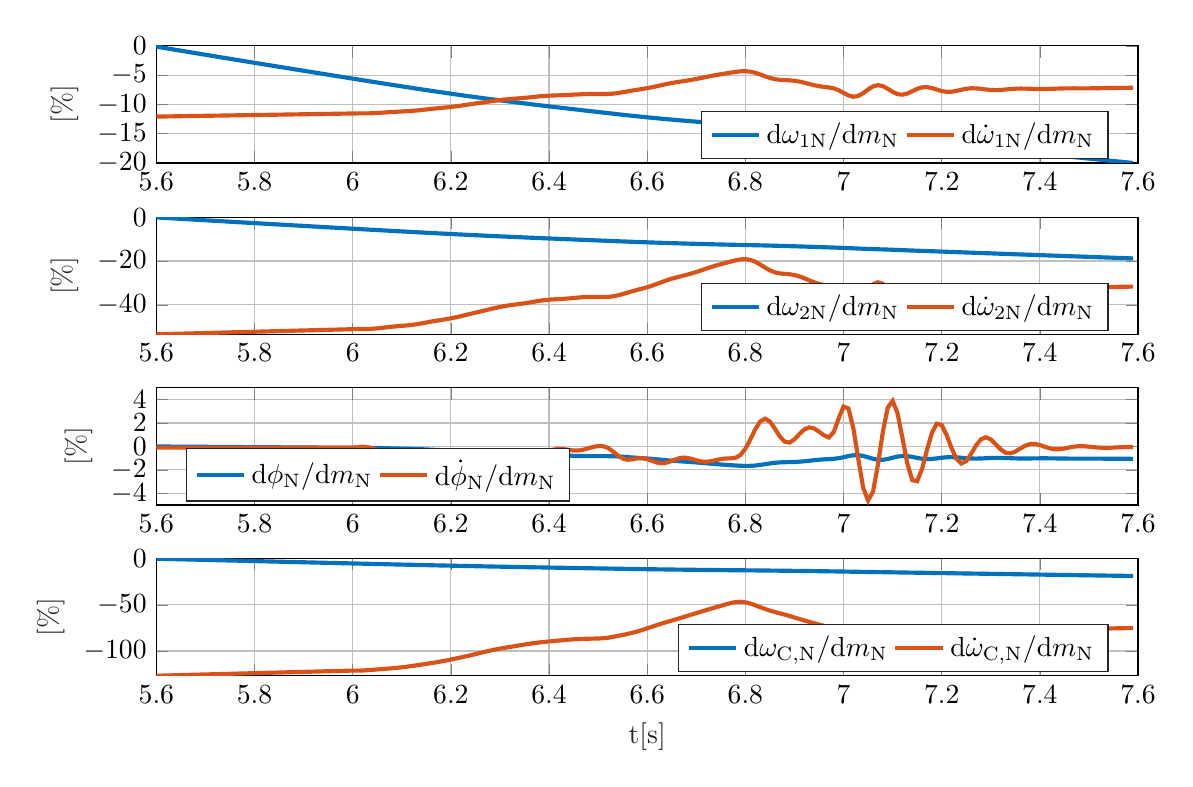
\begin{tikzpicture}

\begin{axis}[%
width=0.959\mwidth,
height=0.186\mheight,
at={(0\mwidth,0.814\mheight)},
scale only axis,
xmin=5.6,
xmax=7.6,
ymin=-20.0293942399798,
ymax=0,
ylabel style={font=\color{white!15!black}},
ylabel={[$\%$]},
axis background/.style={fill=white},
xmajorgrids,
ymajorgrids,
legend style={at={(0.97,0.03)}, anchor=south east, legend columns=2, legend cell align=left, align=left, draw=white!15!black}
]
\addplot [color=mycolor1, line width=1.5pt]
  table[row sep=crcr]{%
5.59	0\\
5.6	-0.139810221040241\\
5.61	-0.279466182537238\\
5.62	-0.4189676049814\\
5.63	-0.558314882035203\\
5.64	-0.697507734480997\\
5.65	-0.836546555773164\\
5.66	-0.975431066985564\\
5.67	-1.11416166136375\\
5.68	-1.25273806027271\\
5.69	-1.39116065674829\\
5.7	-1.52942917244599\\
5.71	-1.66754263141883\\
5.72	-1.80550346365206\\
5.73	-1.94331075321004\\
5.74	-2.08096419236808\\
5.75	-2.21846417251694\\
5.76	-2.35581041610398\\
5.77	-2.49300331541245\\
5.78	-2.63004259342155\\
5.79	-2.76692864225318\\
5.8	-2.90366118507353\\
5.81	-3.04024061361465\\
5.82	-3.1766666511766\\
5.83	-3.31293968920597\\
5.84	-3.44905945131389\\
5.85	-3.5850263288149\\
5.86	-3.72084004569546\\
5.87	-3.8565009931018\\
5.88	-3.99200889529764\\
5.89	-4.12736414315661\\
5.9	-4.262566461156\\
5.91	-4.39761623988926\\
5.92	-4.53252463452141\\
5.93	-4.66729196533479\\
5.94	-4.8019008520116\\
5.95	-4.93636320800014\\
5.96	-5.07067320832231\\
5.97	-5.20482910509364\\
5.98	-5.33882985015196\\
5.99	-5.47266730692488\\
6	-5.6063554322941\\
6.01	-5.73989630305788\\
6.02	-5.87336480887284\\
6.03	-6.00680643608757\\
6.04	-6.1400909308024\\
6.05	-6.2730208618018\\
6.06	-6.40539018884776\\
6.07	-6.53707431210649\\
6.08	-6.6680691657901\\
6.09	-6.79846240219479\\
6.1	-6.92835149710749\\
6.11	-7.05776482298917\\
6.12	-7.18662124607314\\
6.13	-7.31475414256393\\
6.14	-7.44197748128146\\
6.15	-7.56816911204738\\
6.16	-7.69329168176639\\
6.17	-7.8173848432785\\
6.18	-7.94051395246219\\
6.19	-8.06270345998733\\
6.2	-8.18390764043554\\
6.21	-8.30401531821018\\
6.22	-8.42287628265668\\
6.23	-8.54036276298309\\
6.24	-8.6564112400119\\
6.25	-8.7710246267601\\
6.26	-8.88421477035866\\
6.27	-8.99604930493717\\
6.28	-9.10650088322284\\
6.29	-9.21557199367012\\
6.3	-9.32331707979324\\
6.31	-9.42986642969375\\
6.32	-9.53540267184335\\
6.33	-9.64009772901266\\
6.34	-9.74404306529644\\
6.35	-9.84721643183919\\
6.36	-9.94951291486723\\
6.37	-10.0508268960878\\
6.38	-10.1511366542559\\
6.39	-10.2505453433746\\
6.4	-10.3492538716511\\
6.41	-10.4474801535906\\
6.42	-10.5453708970069\\
6.43	-10.6429528121929\\
6.44	-10.7401497513395\\
6.45	-10.83685435644\\
6.46	-10.9330129326722\\
6.47	-11.0286782904549\\
6.48	-11.1240030119179\\
6.49	-11.2191801314204\\
6.5	-11.3143666212183\\
6.51	-11.4096223906845\\
6.52	-11.5048369999983\\
6.53	-11.5996594132069\\
6.54	-11.6935871880734\\
6.55	-11.7861157803096\\
6.56	-11.8769653684323\\
6.57	-11.9660845758372\\
6.58	-12.0535830762377\\
6.59	-12.1395612200712\\
6.6	-12.2239812309499\\
6.61	-12.3066558340964\\
6.62	-12.3873360691942\\
6.63	-12.4658466544944\\
6.64	-12.5421898194048\\
6.65	-12.6165286550104\\
6.66	-12.6891128483074\\
6.67	-12.7601560941607\\
6.68	-12.8297459356005\\
6.69	-12.8978114471024\\
6.7	-12.9641755766412\\
6.71	-13.0286504223226\\
6.72	-13.0911307686945\\
6.73	-13.1516327170445\\
6.74	-13.2102727107401\\
6.75	-13.2672026278388\\
6.76	-13.3225243231426\\
6.77	-13.3763095879861\\
6.78	-13.4285717634385\\
6.79	-13.4794786913101\\
6.8	-13.5296358848656\\
6.81	-13.5800767905016\\
6.82	-13.6320644652319\\
6.83	-13.6868427541489\\
6.84	-13.7451611551319\\
6.85	-13.8070232273794\\
6.86	-13.8717401641417\\
6.87	-13.9382763475781\\
6.88	-14.0057122920578\\
6.89	-14.0736140081793\\
6.9	-14.1421465223472\\
6.91	-14.2119098641841\\
6.92	-14.2836047234782\\
6.93	-14.3577041404141\\
6.94	-14.4342768159538\\
6.95	-14.5130208108556\\
6.96	-14.593455376242\\
6.97	-14.6751658449661\\
6.98	-14.7582070896968\\
6.99	-14.8438847686532\\
7	-14.9340766416692\\
7.01	-15.029727132976\\
7.02	-15.1293505290626\\
7.03	-15.2294312090231\\
7.04	-15.3259093293885\\
7.05	-15.4156956428251\\
7.06	-15.4986654239158\\
7.07	-15.5771508815661\\
7.08	-15.6554056969672\\
7.09	-15.7374297330585\\
7.1	-15.8252784681969\\
7.11	-15.9186329271333\\
7.12	-16.0148804787954\\
7.13	-16.1104173263736\\
7.14	-16.2024697557177\\
7.15	-16.2895728199826\\
7.16	-16.3727903600612\\
7.17	-16.4543561571939\\
7.18	-16.5366992670832\\
7.19	-16.621583912553\\
7.2	-16.7095487067649\\
7.21	-16.7998164024244\\
7.22	-16.8907336630753\\
7.23	-16.9806474759949\\
7.24	-17.0685509681823\\
7.25	-17.1542460491764\\
7.26	-17.2384244898221\\
7.27	-17.3222882674622\\
7.28	-17.4067792872892\\
7.29	-17.492400784828\\
7.3	-17.5791552683964\\
7.31	-17.6665766443867\\
7.32	-17.753904779392\\
7.33	-17.8406047247093\\
7.34	-17.926399316022\\
7.35	-18.0113440970216\\
7.36	-18.0958156817628\\
7.37	-18.1802533141949\\
7.38	-18.2649151496489\\
7.39	-18.349924744811\\
7.4	-18.4352213720252\\
7.41	-18.5206017625856\\
7.42	-18.6058076544373\\
7.43	-18.6907060387476\\
7.44	-18.7752304550141\\
7.45	-18.8594298100492\\
7.46	-18.9434219331101\\
7.47	-19.0273582440928\\
7.48	-19.1113133998887\\
7.49	-19.1953068303513\\
7.5	-19.2792931368649\\
7.51	-19.3632172089515\\
7.52	-19.4469845859881\\
7.53	-19.530592586851\\
7.54	-19.6140231015892\\
7.55	-19.6973004822493\\
7.56	-19.7804562183098\\
7.57	-19.8635074475691\\
7.58	-19.9464861977915\\
7.59	-20.0293942399798\\
};
\addlegendentry{d$\omega_{1\mathrm{N}}/$d$m_\mathrm{N}$}

\addplot [color=mycolor2, line width=1.5pt]
  table[row sep=crcr]{%
5.59	-12.1124811943887\\
5.6	-12.0991087802569\\
5.61	-12.0857413130158\\
5.62	-12.0723787898078\\
5.63	-12.0590212170331\\
5.64	-12.0456685920522\\
5.65	-12.0323209209925\\
5.66	-12.0189782014375\\
5.67	-12.0056404392427\\
5.68	-11.9923076322089\\
5.69	-11.9789797859131\\
5.7	-11.9656568983693\\
5.71	-11.9523390918238\\
5.72	-11.9390261770626\\
5.73	-11.9257181989811\\
5.74	-11.9124151584764\\
5.75	-11.8991170729847\\
5.76	-11.8858239568845\\
5.77	-11.8725358261825\\
5.78	-11.8592526832005\\
5.79	-11.8459745279314\\
5.8	-11.8327013512959\\
5.81	-11.8194331495933\\
5.82	-11.8061699182498\\
5.83	-11.7929116616998\\
5.84	-11.7796583832767\\
5.85	-11.7664100908168\\
5.86	-11.75316678668\\
5.87	-11.7399284739728\\
5.88	-11.7266951502106\\
5.89	-11.7134668150018\\
5.9	-11.7002434654489\\
5.91	-11.6870251024983\\
5.92	-11.6738112732956\\
5.93	-11.6606012097689\\
5.94	-11.6473895780416\\
5.95	-11.6341542570397\\
5.96	-11.6208563314503\\
5.97	-11.6074677367063\\
5.98	-11.5939965670987\\
5.99	-11.58050964368\\
6	-11.5671038142836\\
6.01	-11.5558146619943\\
6.02	-11.5546346146457\\
6.03	-11.5478989501705\\
6.04	-11.5270234654163\\
6.05	-11.4864384215007\\
6.06	-11.4307968642885\\
6.07	-11.3695296773087\\
6.08	-11.3128863582261\\
6.09	-11.2655080999044\\
6.1	-11.2245760041724\\
6.11	-11.1814294747937\\
6.12	-11.1268241374327\\
6.13	-11.0558922997359\\
6.14	-10.9707267481257\\
6.15	-10.8782584343383\\
6.16	-10.7865309002363\\
6.17	-10.7003803240449\\
6.18	-10.6190509004936\\
6.19	-10.5369983363144\\
6.2	-10.4476646315601\\
6.21	-10.3461515269718\\
6.22	-10.2319761340168\\
6.23	-10.1091772470051\\
6.24	-9.9840434056902\\
6.25	-9.86119742517277\\
6.26	-9.7413756140338\\
6.27	-9.62205764397812\\
6.28	-9.50199297705124\\
6.29	-9.38366207639267\\
6.3	-9.2733437182988\\
6.31	-9.17743142249958\\
6.32	-9.09808313665155\\
6.33	-9.0308819171505\\
6.34	-8.96658462303823\\
6.35	-8.89579123170721\\
6.36	-8.81452488391471\\
6.37	-8.72676421946626\\
6.38	-8.64252377949367\\
6.39	-8.57238905686243\\
6.4	-8.52176977332806\\
6.41	-8.48800738635618\\
6.42	-8.46189203123727\\
6.43	-8.43284702652832\\
6.44	-8.39456381471141\\
6.45	-8.34822159195004\\
6.46	-8.30158286550662\\
6.47	-8.26443208629657\\
6.48	-8.24339166720902\\
6.49	-8.23849424838809\\
6.5	-8.24353433537714\\
6.51	-8.24804887881339\\
6.52	-8.23306581240375\\
6.53	-8.17855010885855\\
6.54	-8.07742768540619\\
6.55	-7.94034992417827\\
6.56	-7.78919205271163\\
6.57	-7.64306579068171\\
6.58	-7.50848843532574\\
6.59	-7.37771128870541\\
6.6	-7.23648889375236\\
6.61	-7.07435930628232\\
6.62	-6.89210210052622\\
6.63	-6.70155399015896\\
6.64	-6.51879302239248\\
6.65	-6.35568923770756\\
6.66	-6.21452056104809\\
6.67	-6.0873943536063\\
6.68	-5.96066521489115\\
6.69	-5.82188330062228\\
6.7	-5.66581832038014\\
6.71	-5.49604314222635\\
6.72	-5.32230303588875\\
6.73	-5.15502835928889\\
6.74	-5.00045315612166\\
6.75	-4.85841751496232\\
6.76	-4.72329447333795\\
6.77	-4.58941482959538\\
6.78	-4.46144563879301\\
6.79	-4.36361326409487\\
6.8	-4.33758411539042\\
6.81	-4.41370284568463\\
6.82	-4.60601053710227\\
6.83	-4.88978263763616\\
6.84	-5.20773869035621\\
6.85	-5.49283744206052\\
6.86	-5.69686137372217\\
6.87	-5.80963673433692\\
6.88	-5.86007024545239\\
6.89	-5.89937872798239\\
6.9	-5.97584811572054\\
6.91	-6.11391689423222\\
6.92	-6.30675570225711\\
6.93	-6.52414664188573\\
6.94	-6.72944265213422\\
6.95	-6.89732720099657\\
6.96	-7.02312578650035\\
6.97	-7.12222810437527\\
6.98	-7.27441908333333\\
6.99	-7.58710111884541\\
7	-8.04345147474997\\
7.01	-8.48643078060353\\
7.02	-8.70193071291363\\
7.03	-8.56583473941537\\
7.04	-8.09277085852708\\
7.05	-7.464132448144\\
7.06	-6.93510987157002\\
7.07	-6.72301334864204\\
7.08	-6.88495889465132\\
7.09	-7.3377396519963\\
7.1	-7.8673980432063\\
7.11	-8.25760047183762\\
7.12	-8.35303539535555\\
7.13	-8.15565449465661\\
7.14	-7.76388569585187\\
7.15	-7.35841421296713\\
7.16	-7.10085448694279\\
7.17	-7.05887765868716\\
7.18	-7.21962781687316\\
7.19	-7.48480646969814\\
7.2	-7.73537372128292\\
7.21	-7.87187631376626\\
7.22	-7.84968503937022\\
7.23	-7.70781780053048\\
7.24	-7.51018130203963\\
7.25	-7.33938955184085\\
7.26	-7.25753486390285\\
7.27	-7.27526378522519\\
7.28	-7.35948203499189\\
7.29	-7.46682759301753\\
7.3	-7.54983606096169\\
7.31	-7.57594099197697\\
7.32	-7.54008503348453\\
7.33	-7.46816281179191\\
7.34	-7.38774771069289\\
7.35	-7.32844184023317\\
7.36	-7.3065395931288\\
7.37	-7.31625065279818\\
7.38	-7.34391705950085\\
7.39	-7.37415889754\\
7.4	-7.39142183568378\\
7.41	-7.38815916578493\\
7.42	-7.36543390055424\\
7.43	-7.3336725985006\\
7.44	-7.30185909381554\\
7.45	-7.27836772046911\\
7.46	-7.26776131486108\\
7.47	-7.266620755261\\
7.48	-7.26986835820757\\
7.49	-7.27235990777038\\
7.5	-7.26942532677253\\
7.51	-7.26123193533613\\
7.52	-7.24748113772952\\
7.53	-7.23194760348149\\
7.54	-7.21696687331263\\
7.55	-7.20421004408459\\
7.56	-7.19417608746393\\
7.57	-7.18678095268055\\
7.58	-7.1805960661649\\
7.59	-7.1744100715263\\
};
\addlegendentry{d$\dot{\omega}_{1\mathrm{N}}/$d$m_\mathrm{N}$}

\end{axis}

\begin{axis}[%
width=0.959\mwidth,
height=0.186\mheight,
at={(0\mwidth,0.542\mheight)},
scale only axis,
xmin=5.6,
xmax=7.6,
ymin=-53.4362307924602,
ymax=0,
ylabel style={font=\color{white!15!black}},
ylabel={[$\%$]},
axis background/.style={fill=white},
xmajorgrids,
ymajorgrids,
legend style={at={(0.97,0.03)}, anchor=south east, legend columns=2, legend cell align=left, align=left, draw=white!15!black}
]
\addplot [color=mycolor1, line width=1.5pt]
  table[row sep=crcr]{%
5.59	0\\
5.6	-0.131411319107663\\
5.61	-0.262677645596664\\
5.62	-0.393798716748583\\
5.63	-0.524774902577159\\
5.64	-0.65560594063835\\
5.65	-0.786292200750328\\
5.66	-0.916833420743044\\
5.67	-1.04722997023838\\
5.68	-1.17748158733992\\
5.69	-1.30758864147245\\
5.7	-1.43755087101262\\
5.71	-1.56736735864209\\
5.72	-1.69704038836816\\
5.73	-1.82656909927873\\
5.74	-1.95595320213525\\
5.75	-2.08519306481624\\
5.76	-2.21428842644263\\
5.77	-2.34323965573181\\
5.78	-2.47204649230461\\
5.79	-2.60070930472675\\
5.8	-2.72922783279485\\
5.81	-2.85760244470818\\
5.82	-2.98583288038918\\
5.83	-3.11391950776882\\
5.84	-3.24186206706193\\
5.85	-3.36966092607535\\
5.86	-3.49731582537668\\
5.87	-3.62482713261459\\
5.88	-3.75219458861726\\
5.89	-3.87941856077715\\
5.9	-4.00649879012318\\
5.91	-4.13343564378445\\
5.92	-4.26023960679518\\
5.93	-4.38691098019719\\
5.94	-4.51343342777075\\
5.95	-4.63981814728058\\
5.96	-4.76605966367593\\
5.97	-4.892156334074\\
5.98	-5.0181071732795\\
5.99	-5.14390453351317\\
6	-5.26956153321668\\
6.01	-5.39508012442757\\
6.02	-5.52053069791191\\
6.03	-5.64595600749005\\
6.04	-5.77123362408172\\
6.05	-5.89617797687328\\
6.06	-6.02059540320363\\
6.07	-6.1443687883983\\
6.08	-6.2674943109159\\
6.09	-6.39005435746448\\
6.1	-6.51214054811049\\
6.11	-6.63377955087932\\
6.12	-6.7548951060009\\
6.13	-6.8753305993694\\
6.14	-6.99491117536564\\
6.15	-7.11352202181139\\
6.16	-7.23112802954575\\
6.17	-7.34776646931968\\
6.18	-7.4634987708495\\
6.19	-7.57834791596492\\
6.2	-7.69227092613828\\
6.21	-7.80516330449163\\
6.22	-7.91688386406288\\
6.23	-8.02731250970951\\
6.24	-8.1363895380793\\
6.25	-8.24411768719392\\
6.26	-8.35050809248479\\
6.27	-8.4556243250564\\
6.28	-8.55944068048482\\
6.29	-8.66195949773418\\
6.3	-8.7632319497016\\
6.31	-8.86338049761413\\
6.32	-8.96257679879555\\
6.33	-9.0609824479982\\
6.34	-9.15868341474041\\
6.35	-9.25565878673596\\
6.36	-9.35180995275782\\
6.37	-9.44703763938318\\
6.38	-9.54132143024034\\
6.39	-9.63475828250085\\
6.4	-9.7275370350948\\
6.41	-9.81986251162055\\
6.42	-9.9118726066268\\
6.43	-10.0035924258233\\
6.44	-10.0949503958734\\
6.45	-10.1858456081511\\
6.46	-10.276227593475\\
6.47	-10.3661459897524\\
6.48	-10.4557442129565\\
6.49	-10.5452037011801\\
6.5	-10.6346719967917\\
6.51	-10.7242054101934\\
6.52	-10.8137001360808\\
6.53	-10.9028262264916\\
6.54	-10.991111422697\\
6.55	-11.0780814901961\\
6.56	-11.1634734173868\\
6.57	-11.2472389140419\\
6.58	-11.3294810653809\\
6.59	-11.4102941934307\\
6.6	-11.4896427911663\\
6.61	-11.5673508340786\\
6.62	-11.6431843177921\\
6.63	-11.71697849036\\
6.64	-11.7887354472637\\
6.65	-11.8586084821196\\
6.66	-11.9268322823294\\
6.67	-11.9936077053405\\
6.68	-12.0590170351595\\
6.69	-12.1229936070128\\
6.7	-12.1853710050262\\
6.71	-12.2459726152463\\
6.72	-12.3046995428912\\
6.73	-12.3615669219862\\
6.74	-12.4166842007277\\
6.75	-12.4701941333131\\
6.76	-12.5221924557609\\
6.77	-12.5727466466422\\
6.78	-12.6218692455808\\
6.79	-12.6697180115266\\
6.8	-12.7168620823886\\
6.81	-12.7642728217277\\
6.82	-12.8131374101879\\
6.83	-12.8646249706215\\
6.84	-12.9194399758794\\
6.85	-12.9775857713464\\
6.86	-13.0384149293669\\
6.87	-13.1009540453823\\
6.88	-13.1643388705646\\
6.89	-13.2281614868141\\
6.9	-13.2925770068065\\
6.91	-13.3581494142308\\
6.92	-13.4255373059242\\
6.93	-13.4951853048491\\
6.94	-13.5671579848536\\
6.95	-13.6411715452704\\
6.96	-13.7167741175333\\
6.97	-13.7935759450394\\
6.98	-13.8716286040596\\
6.99	-13.9521593172359\\
7	-14.0369330406279\\
7.01	-14.1268374635122\\
7.02	-14.2204761245238\\
7.03	-14.3145445987239\\
7.04	-14.4052269320168\\
7.05	-14.4896194592493\\
7.06	-14.5676049477044\\
7.07	-14.6413755021287\\
7.08	-14.7149292698135\\
7.09	-14.7920258275688\\
7.1	-14.8745971737895\\
7.11	-14.9623434952111\\
7.12	-15.052809110893\\
7.13	-15.1426067170353\\
7.14	-15.2291292264566\\
7.15	-15.3109996969287\\
7.16	-15.3892180606023\\
7.17	-15.4658839074588\\
7.18	-15.5432803711032\\
7.19	-15.6230656911623\\
7.2	-15.7057461243696\\
7.21	-15.7905911154649\\
7.22	-15.8760466498535\\
7.23	-15.9605590172173\\
7.24	-16.0431818310317\\
7.25	-16.1237289008431\\
7.26	-16.2028504403364\\
7.27	-16.2816762197611\\
7.28	-16.3610915606826\\
7.29	-16.441569467461\\
7.3	-16.5231122977302\\
7.31	-16.6052819577995\\
7.32	-16.6873639782056\\
7.33	-16.7688555465325\\
7.34	-16.8494961487199\\
7.35	-16.9293379917513\\
7.36	-17.0087350651217\\
7.37	-17.0881002258195\\
7.38	-17.1676761208601\\
7.39	-17.2475788844344\\
7.4	-17.327751437015\\
7.41	-17.4080027209767\\
7.42	-17.4880899889946\\
7.43	-17.5678882225521\\
7.44	-17.6473349536691\\
7.45	-17.72647615115\\
7.46	-17.8054225658254\\
7.47	-17.8843165212544\\
7.48	-17.963228189421\\
7.49	-18.0421758329577\\
7.5	-18.1211167805077\\
7.51	-18.1999992322751\\
7.52	-18.2787344022266\\
7.53	-18.3573197703038\\
7.54	-18.4357383144847\\
7.55	-18.5140129239012\\
7.56	-18.5921731963459\\
7.57	-18.6702352400883\\
7.58	-18.7482291588698\\
7.59	-18.8261566173028\\
};
\addlegendentry{d$\omega_{2\mathrm{N}}/$d$m_\mathrm{N}$}

\addplot [color=mycolor2, line width=1.5pt]
  table[row sep=crcr]{%
5.59	-53.4952906307324\\
5.6	-53.4362307924602\\
5.61	-53.3771928023428\\
5.62	-53.3181766477581\\
5.63	-53.2591823569729\\
5.64	-53.2002099183316\\
5.65	-53.1412593588943\\
5.66	-53.0823306679888\\
5.67	-53.0234238714769\\
5.68	-52.9645389596448\\
5.69	-52.9056759571248\\
5.7	-52.8468348551433\\
5.71	-52.7880161936103\\
5.72	-52.7292191368498\\
5.73	-52.670443883145\\
5.74	-52.6116904364612\\
5.75	-52.5529588738034\\
5.76	-52.4942492586753\\
5.77	-52.4355616617712\\
5.78	-52.3768960933458\\
5.79	-52.3182525533676\\
5.8	-52.259631001737\\
5.81	-52.2010314221113\\
5.82	-52.1424537942865\\
5.83	-52.0838981378525\\
5.84	-52.0253644675259\\
5.85	-51.9668528179212\\
5.86	-51.9083631994562\\
5.87	-51.8498956258552\\
5.88	-51.7914500861421\\
5.89	-51.7330265785883\\
5.9	-51.6746250903965\\
5.91	-51.6162456257477\\
5.92	-51.5578861845897\\
5.93	-51.4995433747002\\
5.94	-51.4411936387861\\
5.95	-51.3827392781783\\
5.96	-51.3240084217354\\
5.97	-51.2648771210983\\
5.98	-51.2053811250486\\
5.99	-51.1458155516189\\
6	-51.0866081334037\\
6.01	-51.0367491100542\\
6.02	-51.0315373805289\\
6.03	-51.0017890306315\\
6.04	-50.9095915604298\\
6.05	-50.730345980216\\
6.06	-50.4846026658236\\
6.07	-50.2140135172409\\
6.08	-49.9638458787551\\
6.09	-49.7545977769149\\
6.1	-49.5738194275278\\
6.11	-49.3832609373402\\
6.12	-49.1420941321882\\
6.13	-48.8288206408474\\
6.14	-48.4526833439557\\
6.15	-48.0442930859398\\
6.16	-47.6391745130496\\
6.17	-47.258686813015\\
6.18	-46.8994919395723\\
6.19	-46.5371032846533\\
6.2	-46.1425571613397\\
6.21	-45.6942201983652\\
6.22	-45.1899596978955\\
6.23	-44.6476131675368\\
6.24	-44.0949542117492\\
6.25	-43.5523996909102\\
6.26	-43.0232015433208\\
6.27	-42.4962286314002\\
6.28	-41.965957900849\\
6.29	-41.4433444230869\\
6.3	-40.9561186818505\\
6.31	-40.532517930156\\
6.32	-40.1820728360109\\
6.33	-39.8852757793012\\
6.34	-39.601304033124\\
6.35	-39.2886419960727\\
6.36	-38.9297256994126\\
6.37	-38.5421269758088\\
6.38	-38.1700754739847\\
6.39	-37.8603224753824\\
6.4	-37.6367602472366\\
6.41	-37.4876472228734\\
6.42	-37.3723076413629\\
6.43	-37.2440291372857\\
6.44	-37.0749496968678\\
6.45	-36.870277290338\\
6.46	-36.6642953626309\\
6.47	-36.5002173591978\\
6.48	-36.4072914494679\\
6.49	-36.3856617900309\\
6.5	-36.4079215495266\\
6.51	-36.4278602234711\\
6.52	-36.3616868706081\\
6.53	-36.1209159370324\\
6.54	-35.6743044339835\\
6.55	-35.0688946456665\\
6.56	-34.4012994489881\\
6.57	-33.7559265703328\\
6.58	-33.1615599313641\\
6.59	-32.5839770766187\\
6.6	-31.9602623363978\\
6.61	-31.2442100872872\\
6.62	-30.4392633521806\\
6.63	-29.5976994826771\\
6.64	-28.7905278611315\\
6.65	-28.0701730284044\\
6.66	-27.4466955373224\\
6.67	-26.8852372114237\\
6.68	-26.3255325565184\\
6.69	-25.7125963034954\\
6.7	-25.0233286512818\\
6.71	-24.2735093243027\\
6.72	-23.5061787226215\\
6.73	-22.7674029675751\\
6.74	-22.0847149794554\\
6.75	-21.4574085026235\\
6.76	-20.860631816939\\
6.77	-20.2693466511168\\
6.78	-19.7041652531943\\
6.79	-19.2720843910175\\
6.8	-19.1571255438197\\
6.81	-19.4933071678966\\
6.82	-20.3426423022764\\
6.83	-21.5959339068062\\
6.84	-23.0002003964779\\
6.85	-24.2593512125757\\
6.86	-25.1604316225023\\
6.87	-25.6585088203322\\
6.88	-25.881250576654\\
6.89	-26.0548581689751\\
6.9	-26.3925884866341\\
6.91	-27.0023751451206\\
6.92	-27.8540559786847\\
6.93	-28.8141723503253\\
6.94	-29.7208709496728\\
6.95	-30.4623402316203\\
6.96	-31.0179350585145\\
6.97	-31.4556246789823\\
6.98	-32.1277826390309\\
6.99	-33.5087562064006\\
7	-35.5242470481833\\
7.01	-37.4806840762154\\
7.02	-38.4324487332513\\
7.03	-37.8313750523821\\
7.04	-35.7420682135205\\
7.05	-32.9656598191237\\
7.06	-30.6292090102537\\
7.07	-29.6924756561448\\
7.08	-30.4077150782815\\
7.09	-32.407440635535\\
7.1	-34.7466995469062\\
7.11	-36.4700452420991\\
7.12	-36.8915376587209\\
7.13	-36.0197964788271\\
7.14	-34.2895328428485\\
7.15	-32.4987507172641\\
7.16	-31.361227184528\\
7.17	-31.1758347293196\\
7.18	-31.8857946700688\\
7.19	-33.0569675184947\\
7.2	-34.163608489156\\
7.21	-34.7664780201423\\
7.22	-34.6684693087791\\
7.23	-34.0419065879846\\
7.24	-33.1690365495241\\
7.25	-32.4147274886804\\
7.26	-32.0532127626349\\
7.27	-32.1315133010203\\
7.28	-32.503466798854\\
7.29	-32.977563041592\\
7.3	-33.3441734863231\\
7.31	-33.4594670293347\\
7.32	-33.3011076569145\\
7.33	-32.9834600923481\\
7.34	-32.6283033630734\\
7.35	-32.3663764526886\\
7.36	-32.2696442427053\\
7.37	-32.3125335525838\\
7.38	-32.434723419673\\
7.39	-32.5682877892806\\
7.4	-32.6445302930528\\
7.41	-32.6301205720649\\
7.42	-32.5297534673688\\
7.43	-32.3894783200306\\
7.44	-32.2489726175418\\
7.45	-32.1452219636227\\
7.46	-32.0983783201575\\
7.47	-32.093340989961\\
7.48	-32.1076841671089\\
7.49	-32.1186882021906\\
7.5	-32.10572749985\\
7.51	-32.0695410365565\\
7.52	-32.0088100515041\\
7.53	-31.9402055339165\\
7.54	-31.8740424991612\\
7.55	-31.817701417914\\
7.56	-31.7733860198553\\
7.57	-31.7407250911698\\
7.58	-31.7134092756598\\
7.59	-31.6860885660772\\
};
\addlegendentry{d$\dot{\omega}_{2\mathrm{N}}/$d$m_\mathrm{N}$}

\end{axis}

\begin{axis}[%
width=0.959\mwidth,
height=0.186\mheight,
at={(0\mwidth,0.271\mheight)},
scale only axis,
xmin=5.6,
xmax=7.6,
ymin=-5,
ymax=5,
ylabel style={font=\color{white!15!black}},
ylabel={[$\%$]},
axis background/.style={fill=white},
xmajorgrids,
ymajorgrids,
legend style={at={(0.03,0.03)}, anchor=south west, legend columns=2, legend cell align=left, align=left, draw=white!15!black}
]
\addplot [color=mycolor1, line width=1.5pt]
  table[row sep=crcr]{%
5.59	0\\
5.6	-0.00286146793284332\\
5.61	-0.0057218785906564\\
5.62	-0.0085812308294148\\
5.63	-0.0114395250171215\\
5.64	-0.0142967599923561\\
5.65	-0.0171529361531348\\
5.66	-0.0200080523192472\\
5.67	-0.0228621089181435\\
5.68	-0.0257151047514039\\
5.69	-0.0285670402770578\\
5.7	-0.0314179142796295\\
5.71	-0.0342677080981643\\
5.72	-0.0371164478720934\\
5.73	-0.0399641306458333\\
5.74	-0.0428107563346126\\
5.75	-0.0456563240053936\\
5.76	-0.0485008294794828\\
5.77	-0.0513442705473622\\
5.78	-0.0541866444171547\\
5.79	-0.0570279518089542\\
5.8	-0.0598681927004518\\
5.81	-0.0627073693535062\\
5.82	-0.065545481611699\\
5.83	-0.0683825304407881\\
5.84	-0.0712185140242454\\
5.85	-0.0740534322083354\\
5.86	-0.0768872829267499\\
5.87	-0.079720066652441\\
5.88	-0.0825517822797516\\
5.89	-0.0853824311535057\\
5.9	-0.0882120125388774\\
5.91	-0.0910405276984191\\
5.92	-0.0938680608201499\\
5.93	-0.0966947003910457\\
5.94	-0.099520984955443\\
5.95	-0.102349911778202\\
5.96	-0.105188232740947\\
5.97	-0.108043076230577\\
5.98	-0.11091672512147\\
5.99	-0.113800985577384\\
6	-0.116677617518482\\
6.01	-0.119386756193221\\
6.02	-0.12059724714536\\
6.03	-0.121386308198269\\
6.04	-0.124397937010322\\
6.05	-0.131039232175855\\
6.06	-0.141389563372803\\
6.07	-0.153920829886177\\
6.08	-0.166509941023825\\
6.09	-0.177576591266087\\
6.1	-0.186959418866935\\
6.11	-0.195923218028608\\
6.12	-0.20639851464883\\
6.13	-0.21988043338065\\
6.14	-0.23662399082954\\
6.15	-0.255649125918033\\
6.16	-0.275343978005934\\
6.17	-0.294340323793514\\
6.18	-0.312219669600708\\
6.19	-0.329691014706889\\
6.2	-0.348014285314125\\
6.21	-0.368439790171046\\
6.22	-0.391548207218386\\
6.23	-0.416939198570604\\
6.24	-0.443461601737538\\
6.25	-0.469962070229096\\
6.26	-0.495880109199842\\
6.27	-0.521462884571269\\
6.28	-0.547088047575066\\
6.29	-0.572620974571811\\
6.3	-0.597094143694272\\
6.31	-0.619140868112106\\
6.32	-0.637845506651963\\
6.33	-0.65347433748101\\
6.34	-0.667508486234798\\
6.35	-0.681976774429149\\
6.36	-0.698303340696417\\
6.37	-0.71645359923184\\
6.38	-0.734890655552718\\
6.39	-0.751390590331763\\
6.4	-0.764248568472717\\
6.41	-0.773203516663425\\
6.42	-0.779565367768269\\
6.43	-0.785472029125549\\
6.44	-0.792726079645437\\
6.45	-0.801846742356471\\
6.46	-0.811838729843664\\
6.47	-0.820803470700482\\
6.48	-0.826986224006449\\
6.49	-0.829699054539344\\
6.5	-0.829633314104965\\
6.51	-0.828554930179113\\
6.52	-0.829626759429315\\
6.53	-0.837133036653277\\
6.54	-0.853909814385506\\
6.55	-0.879537497251952\\
6.56	-0.91039605608937\\
6.57	-0.942124939807763\\
6.58	-0.972018543631572\\
6.59	-1.00030750923339\\
6.6	-1.02939073406493\\
6.61	-1.0619128394598\\
6.62	-1.09884711033658\\
6.63	-1.13878915792536\\
6.64	-1.17871499973612\\
6.65	-1.2156646557946\\
6.66	-1.24813483792307\\
6.67	-1.27676434220466\\
6.68	-1.30389149034049\\
6.69	-1.33233291269491\\
6.7	-1.36394669513411\\
6.71	-1.39887766157\\
6.72	-1.43565438619283\\
6.73	-1.47211621351964\\
6.74	-1.50649670787156\\
6.75	-1.53816826568036\\
6.76	-1.56778299280047\\
6.77	-1.59660599782591\\
6.78	-1.62473507445227\\
6.79	-1.64900112488297\\
6.8	-1.66208496848649\\
6.81	-1.65685421828439\\
6.82	-1.62790034386317\\
6.83	-1.57664642747573\\
6.84	-1.51207985261778\\
6.85	-1.44762072682735\\
6.86	-1.39557103485267\\
6.87	-1.36204572904038\\
6.88	-1.34487178072804\\
6.89	-1.33535506584755\\
6.9	-1.32283760596369\\
6.91	-1.29962544566625\\
6.92	-1.26397259447824\\
6.93	-1.21994810130977\\
6.94	-1.17476883665345\\
6.95	-1.13500351311844\\
6.96	-1.10377613719473\\
6.97	-1.07992124776934\\
6.98	-1.05381410434275\\
6.99	-1.00340363283719\\
7	-0.919978071542453\\
7.01	-0.822898570601033\\
7.02	-0.753031320061849\\
7.03	-0.745131460633252\\
7.04	-0.811743560396915\\
7.05	-0.930790041754404\\
7.06	-1.05453176249474\\
7.07	-1.13236245251202\\
7.08	-1.13705378353496\\
7.09	-1.06962406296942\\
7.1	-0.964537238207107\\
7.11	-0.866171507312591\\
7.12	-0.815837797965909\\
7.13	-0.827205475522697\\
7.14	-0.891178213035544\\
7.15	-0.976718155690205\\
7.16	-1.04663826308602\\
7.17	-1.07825782712075\\
7.18	-1.06458193459154\\
7.19	-1.01888881208116\\
7.2	-0.963643258714691\\
7.21	-0.922551921434153\\
7.22	-0.911474326553596\\
7.23	-0.928919072805694\\
7.24	-0.965573746713511\\
7.25	-1.00496669813622\\
7.26	-1.03130963839825\\
7.27	-1.03754761151124\\
7.28	-1.02687655982645\\
7.29	-1.00638366681007\\
7.3	-0.98605355146172\\
7.31	-0.974633223820359\\
7.32	-0.976233060861402\\
7.33	-0.987573816989756\\
7.34	-1.0039096044867\\
7.35	-1.01872300656207\\
7.36	-1.02702675293717\\
7.37	-1.02831420726467\\
7.38	-1.02446934010551\\
7.39	-1.01824787875881\\
7.4	-1.01321156552561\\
7.41	-1.01179023611894\\
7.42	-1.01476856592994\\
7.43	-1.02050436693304\\
7.44	-1.02731504266591\\
7.45	-1.03320861442056\\
7.46	-1.03670005700194\\
7.47	-1.03795837298956\\
7.48	-1.03778928686617\\
7.49	-1.03717989176756\\
7.5	-1.03730908239439\\
7.51	-1.03844739596729\\
7.52	-1.04089830557542\\
7.53	-1.04397368597238\\
7.54	-1.0472058908743\\
7.55	-1.05015344224505\\
7.56	-1.05259710891306\\
7.57	-1.05443950702118\\
7.58	-1.05590682077998\\
7.59	-1.05723271786267\\
};
\addlegendentry{d$\phi_\mathrm{N}/$d$m_\mathrm{N}$}

\addplot [color=mycolor2, line width=1.5pt]
  table[row sep=crcr]{%
5.59	-0.101443326784142\\
5.6	-0.101405880970175\\
5.61	-0.101368358631607\\
5.62	-0.101330884199888\\
5.63	-0.101293334526713\\
5.64	-0.101255831967856\\
5.65	-0.10121825538639\\
5.66	-0.101180725088973\\
5.67	-0.101143121973816\\
5.68	-0.101105564344587\\
5.69	-0.101067935152807\\
5.7	-0.10103035068238\\
5.71	-0.100992279787047\\
5.72	-0.100954739100075\\
5.73	-0.100917257261622\\
5.74	-0.100879826672065\\
5.75	-0.100842249042278\\
5.76	-0.100804602529448\\
5.77	-0.100766801000767\\
5.78	-0.10072900715278\\
5.79	-0.100691170046897\\
5.8	-0.100653428957387\\
5.81	-0.100615679674204\\
5.82	-0.100578002652452\\
5.83	-0.100540262173763\\
5.84	-0.100502536465212\\
5.85	-0.100464717569354\\
5.86	-0.100426916181847\\
5.87	-0.100389051653297\\
5.88	-0.100351240045364\\
5.89	-0.100313391967059\\
5.9	-0.10027560345153\\
5.91	-0.100237770640965\\
5.92	-0.100200793596788\\
5.93	-0.100170048075772\\
5.94	-0.100188250099556\\
5.95	-0.10037841438572\\
5.96	-0.100852100480422\\
5.97	-0.101529621529495\\
5.98	-0.102126399776322\\
5.99	-0.10220988390872\\
6	-0.101604286025514\\
6.01	-0.0807710113182941\\
6.02	-0.0128604531182624\\
6.03	-0.0590772796329837\\
6.04	-0.162183749088303\\
6.05	-0.306904697277795\\
6.06	-0.417047942705917\\
6.07	-0.45790960141509\\
6.08	-0.424547399275582\\
6.09	-0.358596323463667\\
6.1	-0.314244771284313\\
6.11	-0.333179490470105\\
6.12	-0.418749617752895\\
6.13	-0.538793269472743\\
6.14	-0.643495132039095\\
6.15	-0.697215930667589\\
6.16	-0.692228969995163\\
6.17	-0.652178558251977\\
6.18	-0.618192158925556\\
6.19	-0.624094042573633\\
6.2	-0.680029000630994\\
6.21	-0.771652685667824\\
6.22	-0.865126544778546\\
6.23	-0.927578315407856\\
6.24	-0.945239914860986\\
6.25	-0.929759704922162\\
6.26	-0.909702289236876\\
6.27	-0.905769276510274\\
6.28	-0.91015565083478\\
6.29	-0.8947867303025\\
6.3	-0.833024987136905\\
6.31	-0.724787875797689\\
6.32	-0.602254895085217\\
6.33	-0.513536080415186\\
6.34	-0.493817962752119\\
6.35	-0.541842406465328\\
6.36	-0.616969455308915\\
6.37	-0.661312492401575\\
6.38	-0.631939498741612\\
6.39	-0.525959967218049\\
6.4	-0.382181101138325\\
6.41	-0.259427551016726\\
6.42	-0.204516332508652\\
6.43	-0.226301351690097\\
6.44	-0.292678094740875\\
6.45	-0.348957861680581\\
6.46	-0.347969712292177\\
6.47	-0.27590883184599\\
6.48	-0.156728910567462\\
6.49	-0.0386997843253404\\
6.5	0.033075841525183\\
6.51	0.0250992620930155\\
6.52	-0.126149696739947\\
6.53	-0.420821806074558\\
6.54	-0.765163554162212\\
6.55	-1.02738423214513\\
6.56	-1.13234267006497\\
6.57	-1.09930030603854\\
6.58	-1.02120771615422\\
6.59	-0.999228943156152\\
6.6	-1.0793563978662\\
6.61	-1.23278510361685\\
6.62	-1.37870030436244\\
6.63	-1.4371429589171\\
6.64	-1.37863807541181\\
6.65	-1.23299052714719\\
6.66	-1.07221612200297\\
6.67	-0.970729491422061\\
6.68	-0.969716819218728\\
6.69	-1.05832772781083\\
6.7	-1.18417053495426\\
6.71	-1.28279477320448\\
6.72	-1.31071127286922\\
6.73	-1.26289772502838\\
6.74	-1.17002664455673\\
6.75	-1.07901135987271\\
6.76	-1.02896280164524\\
6.77	-1.01617928864586\\
6.78	-0.962950180942568\\
6.79	-0.726513411849274\\
6.8	-0.193800980354092\\
6.81	0.589795466859987\\
6.82	1.45382862886252\\
6.83	2.12421341506566\\
6.84	2.36933812087562\\
6.85	2.12378041067775\\
6.86	1.52833119052998\\
6.87	0.862163250410252\\
6.88	0.409626026199164\\
6.89	0.33116077989287\\
6.9	0.603550862883502\\
6.91	1.05202712298896\\
6.92	1.44925260360601\\
6.93	1.62539407903456\\
6.94	1.53625239676061\\
6.95	1.2635169109959\\
6.96	0.957743942971941\\
6.97	0.769712038760238\\
6.98	1.22714602298062\\
6.99	2.39575413208685\\
7	3.4028700893264\\
7.01	3.23933622842062\\
7.02	1.55491489478125\\
7.03	-1.06904323723583\\
7.04	-3.52146473237528\\
7.05	-4.61640616067641\\
7.06	-3.86779289598544\\
7.07	-1.56726217535532\\
7.08	1.22127981482951\\
7.09	3.30813888479361\\
7.1	3.89153540561606\\
7.11	2.83643574849915\\
7.12	0.715813343869345\\
7.13	-1.47176953610082\\
7.14	-2.87839974461504\\
7.15	-2.96403000396846\\
7.16	-1.91372175895609\\
7.17	-0.30894520074833\\
7.18	1.15949266028134\\
7.19	1.94207893925872\\
7.2	1.82594354236397\\
7.21	0.98328788835546\\
7.22	-0.138499208817952\\
7.23	-1.05340899140323\\
7.24	-1.45237907559185\\
7.25	-1.25012879272186\\
7.26	-0.624159615623335\\
7.27	0.0868929625919987\\
7.28	0.607682927740573\\
7.29	0.782982111016209\\
7.3	0.600734572495915\\
7.31	0.187091088478689\\
7.32	-0.243278494394545\\
7.33	-0.530119897225139\\
7.34	-0.591683667802546\\
7.35	-0.44102986844043\\
7.36	-0.184571742937772\\
7.37	0.0539640501513128\\
7.38	0.200993813037347\\
7.39	0.21861461702554\\
7.4	0.123413447717768\\
7.41	-0.0268188128775158\\
7.42	-0.160338646446538\\
7.43	-0.235429381487578\\
7.44	-0.23511843829427\\
7.45	-0.173607452373278\\
7.46	-0.0869657072902995\\
7.47	-0.0150661795690906\\
7.48	0.0221996982630862\\
7.49	0.0167879550853782\\
7.5	-0.0185587972091163\\
7.51	-0.0621258085032327\\
7.52	-0.0969295131530281\\
7.53	-0.114503284655732\\
7.54	-0.112576847269863\\
7.55	-0.0971016243020796\\
7.56	-0.0760508141133183\\
7.57	-0.0576022258766949\\
7.58	-0.047387713274649\\
7.59	-0.0472144408017388\\
};
\addlegendentry{d$\dot{\phi}_\mathrm{N}/$d$m_\mathrm{N}$}

\end{axis}

\begin{axis}[%
width=0.959\mwidth,
height=0.186\mheight,
at={(0\mwidth,0\mheight)},
scale only axis,
xmin=5.6,
xmax=7.6,
xlabel style={font=\color{white!15!black}},
xlabel={t[s]},
ymin=-126.697507996823,
ymax=0,
ylabel style={font=\color{white!15!black}},
ylabel={[$\%$]},
axis background/.style={fill=white},
xmajorgrids,
ymajorgrids,
legend style={at={(0.97,0.03)}, anchor=south east, legend columns=2, legend cell align=left, align=left, draw=white!15!black}
]
\addplot [color=mycolor1, line width=1.5pt]
  table[row sep=crcr]{%
5.59	0\\
5.6	-0.131411962234403\\
5.61	-0.262678931481211\\
5.62	-0.393800644661217\\
5.63	-0.524777472145666\\
5.64	-0.655609151135747\\
5.65	-0.786296051801315\\
5.66	-0.916837911623472\\
5.67	-1.0472351005699\\
5.68	-1.17748735640114\\
5.69	-1.30759504888183\\
5.7	-1.4375579160514\\
5.71	-1.56737504212322\\
5.72	-1.69704870817501\\
5.73	-1.82657805465376\\
5.74	-1.95596279234172\\
5.75	-2.08520328969212\\
5.76	-2.21429928559889\\
5.77	-2.34325114902991\\
5.78	-2.47205861913463\\
5.79	-2.60072206462753\\
5.8	-2.72924122490155\\
5.81	-2.85761646845871\\
5.82	-2.98584753498782\\
5.83	-3.11393479281366\\
5.84	-3.24187798192389\\
5.85	-3.36967747043891\\
5.86	-3.49733299860528\\
5.87	-3.62484493430629\\
5.88	-3.75221301803358\\
5.89	-3.87943761743949\\
5.9	-4.0065184732743\\
5.91	-4.13345595296881\\
5.92	-4.26026053899802\\
5.93	-4.38693251686471\\
5.94	-4.51345542679887\\
5.95	-4.63984011099893\\
5.96	-4.7660807718947\\
5.97	-4.89217599695605\\
5.98	-5.01812562364313\\
5.99	-5.1439232545681\\
6	-5.26958251639496\\
6.01	-5.395161843483\\
6.02	-5.52080924392551\\
6.03	-5.64610146007466\\
6.04	-5.77108152563735\\
6.05	-5.89560802660184\\
6.06	-6.0197075564382\\
6.07	-6.14336332223866\\
6.08	-6.26658578960869\\
6.09	-6.38933698686413\\
6.1	-6.51155188622627\\
6.11	-6.63313664747166\\
6.12	-6.75400532881071\\
6.13	-6.8740942893103\\
6.14	-6.99337267911497\\
6.15	-7.11182871185726\\
6.16	-7.22944961462117\\
6.17	-7.34620430716902\\
6.18	-7.46203532789278\\
6.19	-7.57686787926525\\
6.2	-7.69062965594603\\
6.21	-7.80325762737706\\
6.22	-7.91470842675953\\
6.23	-8.02495698584084\\
6.24	-8.1339834019006\\
6.25	-8.2417567398016\\
6.26	-8.34820556025398\\
6.27	-8.45333359025804\\
6.28	-8.55713768808272\\
6.29	-8.65970135119889\\
6.3	-8.76115275667348\\
6.31	-8.8616146048552\\
6.32	-8.96116552903442\\
6.33	-9.05982804777645\\
6.34	-9.15758641346667\\
6.35	-9.25442335076151\\
6.36	-9.35035773031738\\
6.37	-9.44545761736585\\
6.38	-9.53982670364888\\
6.39	-9.63357030263189\\
6.4	-9.72676506986446\\
6.41	-9.81944577904564\\
6.42	-9.91161498631172\\
6.43	-10.0032722025378\\
6.44	-10.0944386620607\\
6.45	-10.1851715503407\\
6.46	-10.2755567600922\\
6.47	-10.3656838364847\\
6.48	-10.455626950571\\
6.49	-10.5454280023855\\
6.5	-10.6351041516641\\
6.51	-10.7246148707354\\
6.52	-10.8136727292852\\
6.53	-10.9019473421583\\
6.54	-10.9892374720457\\
6.55	-11.0754498640682\\
6.56	-11.1605387242008\\
6.57	-11.2444000809124\\
6.58	-11.3268683176324\\
6.59	-11.4077453110114\\
6.6	-11.48686259868\\
6.61	-11.5641274250516\\
6.62	-11.6395394046899\\
6.63	-11.713164931163\\
6.64	-11.7850913064843\\
6.65	-11.8553856647468\\
6.66	-11.9240745104797\\
6.67	-11.9911435835832\\
6.68	-12.0565561070754\\
6.69	-12.1202767822627\\
6.7	-12.1822906468545\\
6.71	-12.2426074000645\\
6.72	-12.3012538655204\\
6.73	-12.3582596958366\\
6.74	-12.4136456713232\\
6.75	-12.4674189293632\\
6.76	-12.5195621441984\\
6.77	-12.5701534955219\\
6.78	-12.6194301694987\\
6.79	-12.667962623355\\
6.8	-12.7166468551262\\
6.81	-12.7663230138204\\
6.82	-12.8176855546008\\
6.83	-12.8711112778798\\
6.84	-12.926635114554\\
6.85	-12.9840712866521\\
6.86	-13.0431793632718\\
6.87	-13.1037929706496\\
6.88	-13.1658698558837\\
6.89	-13.2294659039958\\
6.9	-13.2946691134343\\
6.91	-13.3615382462312\\
6.92	-13.4300747145558\\
6.93	-13.5002321880407\\
6.94	-13.5719474695609\\
6.95	-13.6451729054811\\
6.96	-13.7198918547179\\
6.97	-13.7961504308137\\
6.98	-13.8755257610592\\
6.99	-13.9594350229455\\
7	-14.0471204696155\\
7.01	-14.1365525135445\\
7.02	-14.2253222180919\\
7.03	-14.3118057176804\\
7.04	-14.3953989419527\\
7.05	-14.476626547939\\
7.06	-14.5567764505546\\
7.07	-14.6371976963958\\
7.08	-14.7188129011876\\
7.09	-14.8019424803159\\
7.1	-14.8862006495827\\
7.11	-14.9708972382945\\
7.12	-15.0552329113283\\
7.13	-15.1387070022682\\
7.14	-15.2211635668913\\
7.15	-15.302786830013\\
7.16	-15.3840417508663\\
7.17	-15.4653470096669\\
7.18	-15.5469887593193\\
7.19	-15.6290367103047\\
7.2	-15.711381754982\\
7.21	-15.7937911362474\\
7.22	-15.8760041480592\\
7.23	-15.957872031472\\
7.24	-16.0393418359247\\
7.25	-16.1204739001909\\
7.26	-16.201405318037\\
7.27	-16.2822869343333\\
7.28	-16.363208101963\\
7.29	-16.4441930924775\\
7.3	-16.5252094121205\\
7.31	-16.6061836430112\\
7.32	-16.6870218819524\\
7.33	-16.7676845787311\\
7.34	-16.8481475401452\\
7.35	-16.9284252192665\\
7.36	-17.0085639868416\\
7.37	-17.0886190316037\\
7.38	-17.1686202852604\\
7.39	-17.2485743124096\\
7.4	-17.3284719830718\\
7.41	-17.4082893011515\\
7.42	-17.487990915027\\
7.43	-17.5675724005341\\
7.44	-17.6470203538967\\
7.45	-17.726339689914\\
7.46	-17.8055368905166\\
7.47	-17.8846390147487\\
7.48	-17.9636587325803\\
7.49	-18.0425910531473\\
7.5	-18.1214301413557\\
7.51	-18.2001869703579\\
7.52	-18.2788218499762\\
7.53	-18.3573567355281\\
7.54	-18.4357811678521\\
7.55	-18.5141008317551\\
7.56	-18.5923222761695\\
7.57	-18.6704379689594\\
7.58	-18.7484617333846\\
7.59	-18.8263900098999\\
};
\addlegendentry{d$\omega_{\mathrm{C,N}}/$d$m_\mathrm{N}$}

\addplot [color=mycolor2, line width=1.5pt]
  table[row sep=crcr]{%
5.59	-126.837538836586\\
5.6	-126.697507996823\\
5.61	-126.557528756853\\
5.62	-126.417601489718\\
5.63	-126.277725860906\\
5.64	-126.137902243074\\
5.65	-125.99813030151\\
5.66	-125.85841040846\\
5.67	-125.718742228985\\
5.68	-125.579126134901\\
5.69	-125.439561791042\\
5.7	-125.300049568815\\
5.71	-125.160590491239\\
5.72	-125.021182182337\\
5.73	-124.881825659716\\
5.74	-124.742521347669\\
5.75	-124.60326892817\\
5.76	-124.464068769593\\
5.77	-124.324920517504\\
5.78	-124.185824516483\\
5.79	-124.046780411611\\
5.8	-123.907788566972\\
5.81	-123.768848656628\\
5.82	-123.629961064806\\
5.83	-123.491125470185\\
5.84	-123.352342243592\\
5.85	-123.213611043527\\
5.86	-123.07493222149\\
5.87	-122.936305428928\\
5.88	-122.797731018104\\
5.89	-122.659208650717\\
5.9	-122.520738682221\\
5.91	-122.382320776306\\
5.92	-122.243942111034\\
5.93	-122.105578027843\\
5.94	-121.96695910382\\
5.95	-121.827661141561\\
5.96	-121.687617723121\\
5.97	-121.547165425783\\
5.98	-121.406882123165\\
5.99	-121.267475212082\\
6	-121.129064023838\\
6.01	-121.17173852751\\
6.02	-121.045708169633\\
6.03	-120.704154743391\\
6.04	-120.335547675269\\
6.05	-119.898146153493\\
6.06	-119.478006008737\\
6.07	-119.057344938892\\
6.08	-118.627762897856\\
6.09	-118.147244568863\\
6.1	-117.586096810883\\
6.11	-116.934594581155\\
6.12	-116.207681725327\\
6.13	-115.436510840688\\
6.14	-114.647542990535\\
6.15	-113.850176888353\\
6.16	-113.034003600109\\
6.17	-112.175440800879\\
6.18	-111.251526696821\\
6.19	-110.252402329275\\
6.2	-109.184549058863\\
6.21	-108.065569111554\\
6.22	-106.916163000381\\
6.23	-105.747875847033\\
6.24	-104.556797428186\\
6.25	-103.327632832834\\
6.26	-102.045777061831\\
6.27	-100.74577745921\\
6.28	-99.4991953401714\\
6.29	-98.3611896683731\\
6.3	-97.3527168598665\\
6.31	-96.4466361173351\\
6.32	-95.5882636759817\\
6.33	-94.7272108774941\\
6.34	-93.8426238722266\\
6.35	-92.9551106044846\\
6.36	-92.1099366183043\\
6.37	-91.3522454969279\\
6.38	-90.7013770149831\\
6.39	-90.1414967679618\\
6.4	-89.6356987015766\\
6.41	-89.1437144604458\\
6.42	-88.6478473500908\\
6.43	-88.1591376203015\\
6.44	-87.7071381634134\\
6.45	-87.3283205085502\\
6.46	-87.0374969274629\\
6.47	-86.828491142005\\
6.48	-86.6772817681091\\
6.49	-86.549647060727\\
6.5	-86.4361820013616\\
6.51	-86.1757134697271\\
6.52	-85.5649341690762\\
6.53	-84.6883996973936\\
6.54	-83.6812110424159\\
6.55	-82.6218814240019\\
6.56	-81.4971896363309\\
6.57	-80.2427334099995\\
6.58	-78.8036805200859\\
6.59	-77.1779077468446\\
6.6	-75.4211096553139\\
6.61	-73.6206020398785\\
6.62	-71.8573733123104\\
6.63	-70.1766756225444\\
6.64	-68.5763384946154\\
6.65	-67.0232824005082\\
6.66	-65.4736757687479\\
6.67	-63.8951826607253\\
6.68	-62.2780469314055\\
6.69	-60.634950770742\\
6.7	-58.9898057723294\\
6.71	-57.3643523413635\\
6.72	-55.7683260534779\\
6.73	-54.198082129561\\
6.74	-52.6414122694271\\
6.75	-51.0852120274741\\
6.76	-49.5313496304424\\
6.77	-48.0909363323394\\
6.78	-47.0419798341379\\
6.79	-46.7163741805623\\
6.8	-47.2903754366679\\
6.81	-48.6323300802432\\
6.82	-50.5029502076248\\
6.83	-52.557556264432\\
6.84	-54.513612543671\\
6.85	-56.2384803765871\\
6.86	-57.7520937667243\\
6.87	-59.1639110153572\\
6.88	-60.5911927783411\\
6.89	-62.0993695478733\\
6.9	-63.6860572555986\\
6.91	-65.3029911186306\\
6.92	-66.8942252452115\\
6.93	-68.4269349454728\\
6.94	-69.9021662511893\\
6.95	-71.3454103222855\\
6.96	-72.7878353659231\\
6.97	-74.5698211027157\\
6.98	-78.6959325602792\\
6.99	-82.9929057713891\\
7	-85.8109699785231\\
7.01	-86.3066307473392\\
7.02	-84.7173175628716\\
7.03	-82.0160917088669\\
7.04	-79.3232268742935\\
7.05	-77.6018029103262\\
7.06	-77.2160361277498\\
7.07	-78.0316994769645\\
7.08	-79.4493179285985\\
7.09	-80.8132904571382\\
7.1	-81.6122041705847\\
7.11	-81.6364384738992\\
7.12	-80.9865212641577\\
7.13	-80.0149050854872\\
7.14	-79.0756500452263\\
7.15	-78.4841351136238\\
7.16	-78.3357299066378\\
7.17	-78.5448756443576\\
7.18	-78.9403126462503\\
7.19	-79.3093008172219\\
7.2	-79.4943384712485\\
7.21	-79.4299902004301\\
7.22	-79.1487305009084\\
7.23	-78.7674117824885\\
7.24	-78.3960775517686\\
7.25	-78.1310542888457\\
7.26	-78.0144523628136\\
7.27	-78.0183395836082\\
7.28	-78.079256875855\\
7.29	-78.1351389003527\\
7.3	-78.1337740173843\\
7.31	-78.0497879564233\\
7.32	-77.8927256247774\\
7.33	-77.7017724276947\\
7.34	-77.5124440330995\\
7.35	-77.3578182504343\\
7.36	-77.2523450134886\\
7.37	-77.1849491474555\\
7.38	-77.1374424105789\\
7.39	-77.0906687795054\\
7.4	-77.0261186601461\\
7.41	-76.9351235000619\\
7.42	-76.8191753867219\\
7.43	-76.6912758203393\\
7.44	-76.5627094409167\\
7.45	-76.4444558089171\\
7.46	-76.3429114683457\\
7.47	-76.2551584162744\\
7.48	-76.1744315453353\\
7.49	-76.0940844437064\\
7.5	-76.0071222646655\\
7.51	-75.9128817716492\\
7.52	-75.8101249803196\\
7.53	-75.7039234017563\\
7.54	-75.5976407462414\\
7.55	-75.4941268406264\\
7.56	-75.3946137928879\\
7.57	-75.2994989736523\\
7.58	-75.206878595441\\
7.59	-75.1149300406158\\
};
\addlegendentry{d$\dot{\omega}_{\mathrm{C,N}}/$d$m_\mathrm{N}$}

\end{axis}
\end{tikzpicture}%
\caption{Normierte Sensitivitäten der Zustände und deren Ableitungen von $m_\mathrm{veh}$}
\label{fig:Sens_m}
\end{figure}

\subsection{Sensitivität des Zustandes $\pmb{x}$ von $\zeta$}
Die Sensitivität von \eqref{eq:sys_nl23} vom Parameter $\zeta$ ergibt sich mit \eqref{eq:Sens_eq} zu
\begin{align}
\dot{\pmb{S}}_{\zeta} = \frac{\partial\pmb{f}(t,\pmb{x}(t,\pmb{p}),\pmb{p})}{\partial \pmb{x}} \pmb{S}_{\zeta}
+ \begin{bmatrix} 0 \\ 0 \\ 0 \\ \frac{-m_\mathrm{veh}\,(170\,\cos(\zeta) - 55,8\,f_\mathrm{Roll}\,\omega_\mathrm{C}\,\sin(\zeta))}{5,69\,m_\mathrm{veh} + 337}\end{bmatrix}.
\end{align}

\begin{figure}
\centering
\newlength\zheight 
\setlength\zheight{8cm}
\newlength\zwidth 
\setlength\zwidth{13cm}
% This file was created by matlab2tikz.
%
%The latest updates can be retrieved from
%  http://www.mathworks.com/matlabcentral/fileexchange/22022-matlab2tikz-matlab2tikz
%where you can also make suggestions and rate matlab2tikz.
%
\definecolor{mycolor1}{rgb}{0.00000,0.44700,0.74100}%
\definecolor{mycolor2}{rgb}{0.85000,0.32500,0.09800}%
%
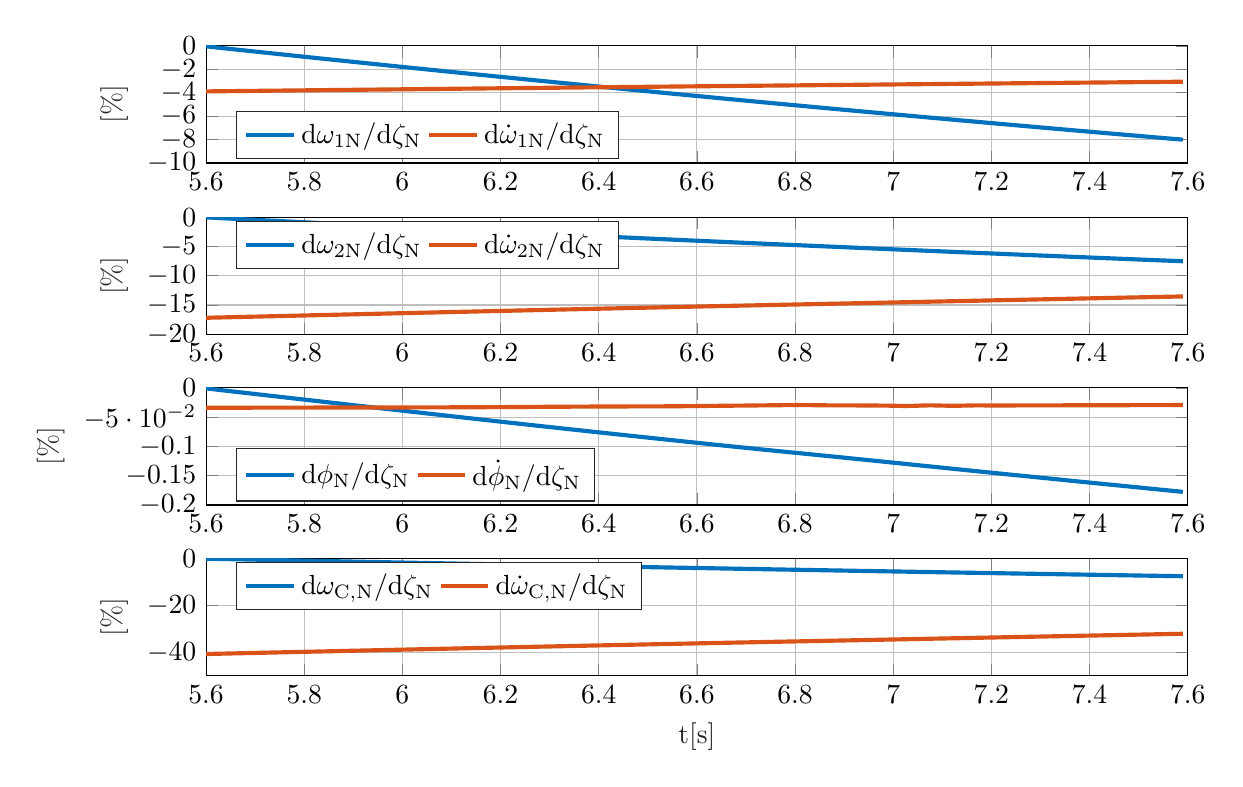
\begin{tikzpicture}

\begin{axis}[%
width=0.959\zwidth,
height=0.186\zheight,
at={(0\zwidth,0.814\zheight)},
scale only axis,
xmin=5.6,
xmax=7.6,
ymin=-10,
ymax=0,
ylabel style={font=\color{white!15!black}},
ylabel={[$\%$]},
axis background/.style={fill=white},
xmajorgrids,
ymajorgrids,
legend style={at={(0.03,0.03)}, anchor=south west, legend columns=2, legend cell align=left, align=left, draw=white!15!black}
]
\addplot [color=mycolor1, line width=1.5pt]
  table[row sep=crcr]{%
5.59	0\\
5.6	-0.044945703992688\\
5.61	-0.0898397666666252\\
5.62	-0.134682095466796\\
5.63	-0.179472823188029\\
5.64	-0.224211857376064\\
5.65	-0.268899330750271\\
5.66	-0.313535150956986\\
5.67	-0.358119450639846\\
5.68	-0.402652137545643\\
5.69	-0.447133344242007\\
5.7	-0.491562978576001\\
5.71	-0.535940714904561\\
5.72	-0.58026736756555\\
5.73	-0.624542631001466\\
5.74	-0.668766403245242\\
5.75	-0.712938816305\\
5.76	-0.757059778299043\\
5.77	-0.801129421506355\\
5.78	-0.845147654212304\\
5.79	-0.889114608639083\\
5.8	-0.933030193156346\\
5.81	-0.97689453987462\\
5.82	-1.0207075572291\\
5.83	-1.06446937723152\\
5.84	-1.10817990841199\\
5.85	-1.15183928271298\\
5.86	-1.19544740877786\\
5.87	-1.23900441848349\\
5.88	-1.28251022057883\\
5.89	-1.3259649468623\\
5.9	-1.36936850617716\\
5.91	-1.41272103023711\\
5.92	-1.45602625212659\\
5.93	-1.49928428028689\\
5.94	-1.542489310731\\
5.95	-1.5856453894372\\
5.96	-1.62875075529345\\
5.97	-1.67180513745478\\
5.98	-1.71480855750988\\
5.99	-1.7577585872647\\
6	-1.80065968057166\\
6.01	-1.84351031580852\\
6.02	-1.88631001395705\\
6.03	-1.92905886855802\\
6.04	-1.97175655586622\\
6.05	-2.01440342096949\\
6.06	-2.05699987805818\\
6.07	-2.09954559342704\\
6.08	-2.14204060636044\\
6.09	-2.18448496038071\\
6.1	-2.22687869460905\\
6.11	-2.26922184511327\\
6.12	-2.31151444922785\\
6.13	-2.35375655031956\\
6.14	-2.39594820167438\\
6.15	-2.43808946154562\\
6.16	-2.48018039390069\\
6.17	-2.52222106257538\\
6.18	-2.56421153074752\\
6.19	-2.60615185926518\\
6.2	-2.64804210702314\\
6.21	-2.68988233906092\\
6.22	-2.73167262885907\\
6.23	-2.77341305571564\\
6.24	-2.81510370449221\\
6.25	-2.85674466182303\\
6.26	-2.89833517837814\\
6.27	-2.93987701610534\\
6.28	-2.98136942001216\\
6.29	-3.02281247627788\\
6.3	-3.06420627250732\\
6.31	-3.10555089048557\\
6.32	-3.14684640503208\\
6.33	-3.18809288329303\\
6.34	-3.22929038617481\\
6.35	-3.27043897284302\\
6.36	-3.31153870607115\\
6.37	-3.35258965450892\\
6.38	-3.39359189059612\\
6.39	-3.4345454851866\\
6.4	-3.47545050177322\\
6.41	-3.51630699340667\\
6.42	-3.55711500394087\\
6.43	-3.59787457297755\\
6.44	-3.63858574158329\\
6.45	-3.67924855585184\\
6.46	-3.71986306633925\\
6.47	-3.76042932384144\\
6.48	-3.80094737395113\\
6.49	-3.8414172532763\\
6.5	-3.88183887078191\\
6.51	-3.92221221261783\\
6.52	-3.96253763198955\\
6.53	-4.00281508334993\\
6.54	-4.04304451056621\\
6.55	-4.08322583857767\\
6.56	-4.12335954119602\\
6.57	-4.16344554360341\\
6.58	-4.20348396004987\\
6.59	-4.24347490005832\\
6.6	-4.28341847221072\\
6.61	-4.32331479201733\\
6.62	-4.36316398822495\\
6.63	-4.40296620416692\\
6.64	-4.44272158519556\\
6.65	-4.48243027319373\\
6.66	-4.52209240127417\\
6.67	-4.56170808888968\\
6.68	-4.60127744911321\\
6.69	-4.6408005959343\\
6.7	-4.6802776503752\\
6.71	-4.71970874446486\\
6.72	-4.75909401944586\\
6.73	-4.79843361975218\\
6.74	-4.83772768680566\\
6.75	-4.87697635527695\\
6.76	-4.9161793219178\\
6.77	-4.9553375759735\\
6.78	-4.99445080687109\\
6.79	-5.03351835329343\\
6.8	-5.07254012659709\\
6.81	-5.11151874223388\\
6.82	-5.15045274720747\\
6.83	-5.18934189760276\\
6.84	-5.22818604439243\\
6.85	-5.26698501496273\\
6.86	-5.30573865575264\\
6.87	-5.34444686310295\\
6.88	-5.38310959053224\\
6.89	-5.42172683113298\\
6.9	-5.46029858529996\\
6.91	-5.4988248298501\\
6.92	-5.53730550185265\\
6.93	-5.57574050243072\\
6.94	-5.61412971523618\\
6.95	-5.65247303022761\\
6.96	-5.6907703598913\\
6.97	-5.72902155419135\\
6.98	-5.76722655061125\\
6.99	-5.80538534125524\\
7	-5.84349795996407\\
7.01	-5.8815633183078\\
7.02	-5.91958140352306\\
7.03	-5.95755338035772\\
7.04	-5.99547842319015\\
7.05	-6.03335632164029\\
7.06	-6.07118861981488\\
7.07	-6.10897425602658\\
7.08	-6.14671517992658\\
7.09	-6.18440986386628\\
7.1	-6.22205913310407\\
7.11	-6.25966210798164\\
7.12	-6.29721771549616\\
7.13	-6.3347275620655\\
7.14	-6.37219096750693\\
7.15	-6.40960666004679\\
7.16	-6.44697655911584\\
7.17	-6.4843020816546\\
7.18	-6.52158159972655\\
7.19	-6.55881608444028\\
7.2	-6.59600476941682\\
7.21	-6.63314747276347\\
7.22	-6.67024289527726\\
7.23	-6.70729352337727\\
7.24	-6.7442982478827\\
7.25	-6.78125699303573\\
7.26	-6.8181686811093\\
7.27	-6.85503393663357\\
7.28	-6.89185569454378\\
7.29	-6.92863251485293\\
7.3	-6.96536374826917\\
7.31	-7.0020493553266\\
7.32	-7.03868704194831\\
7.33	-7.07528138018902\\
7.34	-7.11183027938533\\
7.35	-7.14833234278885\\
7.36	-7.18478672838925\\
7.37	-7.22119676057664\\
7.38	-7.25756415078415\\
7.39	-7.29388633758086\\
7.4	-7.33016323542594\\
7.41	-7.36639484313196\\
7.42	-7.40257835146193\\
7.43	-7.43871936585839\\
7.44	-7.47481529399544\\
7.45	-7.51086608934067\\
7.46	-7.54686835396161\\
7.47	-7.5828263595473\\
7.48	-7.61874141854861\\
7.49	-7.65460911080445\\
7.5	-7.69042864006661\\
7.51	-7.72620916039267\\
7.52	-7.76193638208817\\
7.53	-7.79762242644786\\
7.54	-7.83326358826925\\
7.55	-7.86886151722416\\
7.56	-7.90441756584187\\
7.57	-7.93992662227347\\
7.58	-7.97539327384807\\
7.59	-8.01081523293402\\
};
\addlegendentry{d$\omega_{1\mathrm{N}}/$d$\zeta_\mathrm{N}$}

\addplot [color=mycolor2, line width=1.5pt]
  table[row sep=crcr]{%
5.59	-3.89399544161951\\
5.6	-3.88951871391663\\
5.61	-3.88504372964221\\
5.62	-3.88057048869124\\
5.63	-3.87609899223312\\
5.64	-3.87162924023712\\
5.65	-3.86716123378129\\
5.66	-3.86269497290835\\
5.67	-3.85823045860431\\
5.68	-3.85376769098497\\
5.69	-3.84930667094448\\
5.7	-3.84484739867144\\
5.71	-3.84038991421432\\
5.72	-3.83593415443879\\
5.73	-3.83148013499527\\
5.74	-3.82702785715959\\
5.75	-3.82257732508624\\
5.76	-3.81812854336069\\
5.77	-3.81368151558184\\
5.78	-3.8092362433754\\
5.79	-3.8047927265687\\
5.8	-3.80035096415407\\
5.81	-3.79591095484434\\
5.82	-3.79147269820764\\
5.83	-3.78703619423597\\
5.84	-3.78260144399872\\
5.85	-3.77816844833411\\
5.86	-3.77373720862933\\
5.87	-3.76930772530918\\
5.88	-3.76487999925072\\
5.89	-3.76045403024386\\
5.9	-3.75602981892802\\
5.91	-3.75160736497095\\
5.92	-3.74718651635695\\
5.93	-3.7427671269498\\
5.94	-3.7383493348955\\
5.95	-3.73393308420237\\
5.96	-3.72951850298115\\
5.97	-3.72510569538542\\
5.98	-3.72069473810614\\
5.99	-3.71628577602629\\
6	-3.71187864092863\\
6.01	-3.70747326589323\\
6.02	-3.70306929139734\\
6.03	-3.6986665016989\\
6.04	-3.6942654149309\\
6.05	-3.68986682976082\\
6.06	-3.68547158174196\\
6.07	-3.6810801984706\\
6.08	-3.67669272227378\\
6.09	-3.67230882690183\\
6.1	-3.66792813968142\\
6.11	-3.66355055635924\\
6.12	-3.65917640720749\\
6.13	-3.65480636904884\\
6.14	-3.65044120851056\\
6.15	-3.64608144860669\\
6.16	-3.64172728383532\\
6.17	-3.63737860400877\\
6.18	-3.63303519500655\\
6.19	-3.62869700065023\\
6.2	-3.62436424261205\\
6.21	-3.62003740905875\\
6.22	-3.61571715129238\\
6.23	-3.61140403669745\\
6.24	-3.60709838091456\\
6.25	-3.60280023530564\\
6.26	-3.59850966008729\\
6.27	-3.59422638456782\\
6.28	-3.58995059807891\\
6.29	-3.58568233801727\\
6.3	-3.58142142779831\\
6.31	-3.5771673706987\\
6.32	-3.57291944671346\\
6.33	-3.56867697357259\\
6.34	-3.56443959996456\\
6.35	-3.56020744910621\\
6.36	-3.55598099247911\\
6.37	-3.55176070694948\\
6.38	-3.54754671541499\\
6.39	-3.54333860822921\\
6.4	-3.53913555357969\\
6.41	-3.53493663873638\\
6.42	-3.53074124812871\\
6.43	-3.52654927663167\\
6.44	-3.5223610604668\\
6.45	-3.51817707157259\\
6.46	-3.51399755051498\\
6.47	-3.50982227450239\\
6.48	-3.5056505825738\\
6.49	-3.50148163200256\\
6.5	-3.49731473716363\\
6.51	-3.49314963559173\\
6.52	-3.48898680043683\\
6.53	-3.4848278088606\\
6.54	-3.48067494591362\\
6.55	-3.47653054521707\\
6.56	-3.47239592589058\\
6.57	-3.46827141295441\\
6.58	-3.46415659778379\\
6.59	-3.46005111219038\\
6.6	-3.45595521324574\\
6.61	-3.45186983758748\\
6.62	-3.44779620301549\\
6.63	-3.44373518961121\\
6.64	-3.43968685814627\\
6.65	-3.43565052635926\\
6.66	-3.43162511015514\\
6.67	-3.42760968800189\\
6.68	-3.4236039222113\\
6.69	-3.41960821149057\\
6.7	-3.41562344975532\\
6.71	-3.41165058406614\\
6.72	-3.4076901774599\\
6.73	-3.40374222548321\\
6.74	-3.39980625146493\\
6.75	-3.39588160924228\\
6.76	-3.39196792000385\\
6.77	-3.38806484312652\\
6.78	-3.38417239425555\\
6.79	-3.38028984930336\\
6.8	-3.37641428505386\\
6.81	-3.37254043605126\\
6.82	-3.36866213229465\\
6.83	-3.36477314998213\\
6.84	-3.36086964671643\\
6.85	-3.35695144576054\\
6.86	-3.35302181070907\\
6.87	-3.34908576620075\\
6.88	-3.34514781294463\\
6.89	-3.34121007990021\\
6.9	-3.33727172913527\\
6.91	-3.33332973980706\\
6.92	-3.32938055453741\\
6.93	-3.32542171742545\\
6.94	-3.32145277249434\\
6.95	-3.31747511918754\\
6.96	-3.31349107041627\\
6.97	-3.30950263591963\\
6.98	-3.30550944862576\\
6.99	-3.30150468054594\\
7	-3.29747849223202\\
7.01	-3.29342586859521\\
7.02	-3.2893543742003\\
7.03	-3.28528218466438\\
7.04	-3.28123052677097\\
7.05	-3.27721573115068\\
7.06	-3.27323865233668\\
7.07	-3.26928737389703\\
7.08	-3.26533959362946\\
7.09	-3.26137429367575\\
7.1	-3.25738039199565\\
7.11	-3.25335933032673\\
7.12	-3.24932472258048\\
7.13	-3.24529550471252\\
7.14	-3.2412864817229\\
7.15	-3.2373057224405\\
7.16	-3.23334777855357\\
7.17	-3.22940084062943\\
7.18	-3.2254520299094\\
7.19	-3.22149174855007\\
7.2	-3.21751694224798\\
7.21	-3.21353158997193\\
7.22	-3.20954452611413\\
7.23	-3.20556458117573\\
7.24	-3.20159732528572\\
7.25	-3.19764399313894\\
7.26	-3.19370105979065\\
7.27	-3.18976207678246\\
7.28	-3.18582175366972\\
7.29	-3.18187727464645\\
7.3	-3.1779284990403\\
7.31	-3.17397786457705\\
7.32	-3.17002963099509\\
7.33	-3.16608662060757\\
7.34	-3.16215051232041\\
7.35	-3.15822115198778\\
7.36	-3.15429661463531\\
7.37	-3.15037433660891\\
7.38	-3.14645272308415\\
7.39	-3.1425310815737\\
7.4	-3.13860966410256\\
7.41	-3.13468958204747\\
7.42	-3.13077246797895\\
7.43	-3.12685891065621\\
7.44	-3.12294942112966\\
7.45	-3.11904374443314\\
7.46	-3.11514138639393\\
7.47	-3.1112413429251\\
7.48	-3.10734306155713\\
7.49	-3.1034465611503\\
7.5	-3.09955217374046\\
7.51	-3.09565980106647\\
7.52	-3.09177063035473\\
7.53	-3.08788415879222\\
7.54	-3.08400064185992\\
7.55	-3.08011984644078\\
7.56	-3.07624147821042\\
7.57	-3.07236562897651\\
7.58	-3.06849195172669\\
7.59	-3.06462054890528\\
};
\addlegendentry{d$\dot{\omega}_{1\mathrm{N}}/$d$\zeta_\mathrm{N}$}

\end{axis}

\begin{axis}[%
width=0.959\zwidth,
height=0.186\zheight,
at={(0\zwidth,0.542\zheight)},
scale only axis,
xmin=5.6,
xmax=7.6,
ymin=-20,
ymax=0,
ylabel style={font=\color{white!15!black}},
ylabel={[$\%$]},
axis background/.style={fill=white},
xmajorgrids,
ymajorgrids,
legend style={at={(0.03,0.97)}, anchor=north west, legend columns=2, legend cell align=left, align=left, draw=white!15!black}
]
\addplot [color=mycolor1, line width=1.5pt]
  table[row sep=crcr]{%
5.59	0\\
5.6	-0.0422456541872118\\
5.61	-0.0844427693350979\\
5.62	-0.126591258448752\\
5.63	-0.168691246345544\\
5.64	-0.210742646125268\\
5.65	-0.252745582534368\\
5.66	-0.294699968767194\\
5.67	-0.336605929499008\\
5.68	-0.378463378018576\\
5.69	-0.420272438929723\\
5.7	-0.462033025615463\\
5.71	-0.503744831995268\\
5.72	-0.545408623486829\\
5.73	-0.587024112888574\\
5.74	-0.628591204358952\\
5.75	-0.670110021975891\\
5.76	-0.711580479377355\\
5.77	-0.753002700895856\\
5.78	-0.794376600326384\\
5.79	-0.835702301948078\\
5.8	-0.876979719635152\\
5.81	-0.918208977561775\\
5.82	-0.95938998966377\\
5.83	-1.00052288002247\\
5.84	-1.04160756266288\\
5.85	-1.08264416160124\\
5.86	-1.12363259096901\\
5.87	-1.16457297472076\\
5.88	-1.20546522708722\\
5.89	-1.2463094719492\\
5.9	-1.28710562362608\\
5.91	-1.32785380591904\\
5.92	-1.36855752765274\\
5.93	-1.40921689075399\\
5.94	-1.44982643990215\\
5.95	-1.49038997801904\\
5.96	-1.53090584978894\\
5.97	-1.57137380063753\\
5.98	-1.61179385085657\\
5.99	-1.65216371812235\\
6	-1.6924875887284\\
6.01	-1.73276403246178\\
6.02	-1.7729925990806\\
6.03	-1.8131733765063\\
6.04	-1.85330606044221\\
6.05	-1.89339097524551\\
6.06	-1.93342851022464\\
6.07	-1.97341835172121\\
6.08	-2.01336053665967\\
6.09	-2.05325510594778\\
6.1	-2.09310209635661\\
6.11	-2.13290154178723\\
6.12	-2.17265347733131\\
6.13	-2.21235794375043\\
6.14	-2.25201499112947\\
6.15	-2.29162467422228\\
6.16	-2.3311870531535\\
6.17	-2.37070218792409\\
6.18	-2.41017013791653\\
6.19	-2.44959096032356\\
6.2	-2.48896471050192\\
6.21	-2.52829144958399\\
6.22	-2.56757124663607\\
6.23	-2.60680417619248\\
6.24	-2.64599031801688\\
6.25	-2.68512975353909\\
6.26	-2.72422177844407\\
6.27	-2.76326804883311\\
6.28	-2.80226785506883\\
6.29	-2.84122127815343\\
6.3	-2.88012840042898\\
6.31	-2.91898929876746\\
6.32	-2.95780404349364\\
6.33	-2.99657269771999\\
6.34	-3.03529531869401\\
6.35	-3.07397196202705\\
6.36	-3.11260268672154\\
6.37	-3.15118755730319\\
6.38	-3.18972664186005\\
6.39	-3.22822000698953\\
6.4	-3.26666771237026\\
6.41	-3.30506980786596\\
6.42	-3.34342633469611\\
6.43	-3.38173733008341\\
6.44	-3.42000283262742\\
6.45	-3.45822288565289\\
6.46	-3.49639753667878\\
6.47	-3.53452683344951\\
6.48	-3.57261081881888\\
6.49	-3.6106495271957\\
6.5	-3.64864287301373\\
6.51	-3.68659084325488\\
6.52	-3.7244937699063\\
6.53	-3.76235161015705\\
6.54	-3.80016431124645\\
6.55	-3.83793180262295\\
6.56	-3.87565452963469\\
6.57	-3.9133324219584\\
6.58	-3.95096558698071\\
6.59	-3.98855412764507\\
6.6	-4.02609814601057\\
6.61	-4.06359775064834\\
6.62	-4.10105306257089\\
6.63	-4.13846421650103\\
6.64	-4.17583134905922\\
6.65	-4.21315459360493\\
6.66	-4.25043407525433\\
6.67	-4.28766990628426\\
6.68	-4.32486219297497\\
6.69	-4.36201104246824\\
6.7	-4.39911656851609\\
6.71	-4.436178895216\\
6.72	-4.47319815532561\\
6.73	-4.51017448460223\\
6.74	-4.547108015972\\
6.75	-4.58399887601539\\
6.76	-4.62084677970138\\
6.77	-4.65765265684774\\
6.78	-4.69441621553874\\
6.79	-4.73113683418496\\
6.8	-4.76781442946806\\
6.81	-4.80445145972028\\
6.82	-4.84104655923202\\
6.83	-4.87759949874099\\
6.84	-4.91411013817252\\
6.85	-4.95057831528236\\
6.86	-4.98700388573447\\
6.87	-5.02338675209682\\
6.88	-5.05972687068029\\
6.89	-5.09602423499231\\
6.9	-5.13227884540396\\
6.91	-5.16849068012483\\
6.92	-5.20465968000467\\
6.93	-5.24078575210648\\
6.94	-5.27686878707155\\
6.95	-5.31290868146908\\
6.96	-5.3489053530426\\
6.97	-5.38485866076941\\
6.98	-5.42076854588859\\
6.99	-5.45663500097872\\
7	-5.4924580578476\\
7.01	-5.52823669345118\\
7.02	-5.56397089579284\\
7.03	-5.59966175964987\\
7.04	-5.63530850899869\\
7.05	-5.67091094609753\\
7.06	-5.70647052229308\\
7.07	-5.74198623967739\\
7.08	-5.77745993077909\\
7.09	-5.81289015972091\\
7.1	-5.84827770218502\\
7.11	-5.88362173135733\\
7.12	-5.91892123869416\\
7.13	-5.95417773411007\\
7.14	-5.98939057828336\\
7.15	-6.02455857584039\\
7.16	-6.05968353090481\\
7.17	-6.09476677529643\\
7.18	-6.12980677887473\\
7.19	-6.16480445441033\\
7.2	-6.19975908156337\\
7.21	-6.23467048936812\\
7.22	-6.26953745666939\\
7.23	-6.30436232051814\\
7.24	-6.33914403836604\\
7.25	-6.37388253900632\\
7.26	-6.40857680945484\\
7.27	-6.44322743672402\\
7.28	-6.47783717943698\\
7.29	-6.5124046841119\\
7.3	-6.54692934046224\\
7.31	-6.58141111139296\\
7.32	-6.61584784064058\\
7.33	-6.65024382560009\\
7.34	-6.68459710120171\\
7.35	-6.71890635460478\\
7.36	-6.75317079438154\\
7.37	-6.78739354521404\\
7.38	-6.8215762157235\\
7.39	-6.85571639835333\\
7.4	-6.88981401270146\\
7.41	-6.92386905765178\\
7.42	-6.95787889272825\\
7.43	-6.99184878663438\\
7.44	-7.02577630277457\\
7.45	-7.05966139741178\\
7.46	-7.09350087673953\\
7.47	-7.1272987558312\\
7.48	-7.16105626829399\\
7.49	-7.19476925950177\\
7.5	-7.22843698103984\\
7.51	-7.26206803704863\\
7.52	-7.29564899626696\\
7.53	-7.32919125181989\\
7.54	-7.36269132108973\\
7.55	-7.3961507546466\\
7.56	-7.42957082376848\\
7.57	-7.46294672369358\\
7.58	-7.49628276617369\\
7.59	-7.5295768010034\\
};
\addlegendentry{d$\omega_{2\mathrm{N}}/$d$\zeta_\mathrm{N}$}

\addplot [color=mycolor2, line width=1.5pt]
  table[row sep=crcr]{%
5.59	-17.1979972163496\\
5.6	-17.1782255572076\\
5.61	-17.1584615979917\\
5.62	-17.1387053382383\\
5.63	-17.1189567831121\\
5.64	-17.0992159324778\\
5.65	-17.0794827910958\\
5.66	-17.0597573591553\\
5.67	-17.0400396410107\\
5.68	-17.0203296371742\\
5.69	-17.0006273515942\\
5.7	-16.9809327851034\\
5.71	-16.9612461145783\\
5.72	-16.9415670611832\\
5.73	-16.9218956940386\\
5.74	-16.9022320187797\\
5.75	-16.8825760537544\\
5.76	-16.8629278192151\\
5.77	-16.8432873310561\\
5.78	-16.8236545964579\\
5.79	-16.8040296146574\\
5.8	-16.7844123812047\\
5.81	-16.7648028904144\\
5.82	-16.7452011403797\\
5.83	-16.7256071310649\\
5.84	-16.7060208671931\\
5.85	-16.6864423524661\\
5.86	-16.6668715930108\\
5.87	-16.6473085907034\\
5.88	-16.6277533494171\\
5.89	-16.6082058682244\\
5.9	-16.5886661499493\\
5.91	-16.569134193124\\
5.92	-16.5496093263649\\
5.93	-16.5300909042557\\
5.94	-16.5105795369232\\
5.95	-16.4910749770781\\
5.96	-16.4715777905273\\
5.97	-16.4520884372688\\
5.98	-16.4326072560123\\
5.99	-16.4131348866392\\
6	-16.393670586211\\
6.01	-16.3742140591732\\
6.02	-16.3547637176777\\
6.03	-16.3353186088907\\
6.04	-16.3158810211689\\
6.05	-16.2964544818611\\
6.06	-16.2770426812242\\
6.07	-16.2576479494101\\
6.08	-16.2382704733572\\
6.09	-16.2189088121704\\
6.1	-16.199561319922\\
6.11	-16.1802275361723\\
6.12	-16.1609089195835\\
6.13	-16.1416084593713\\
6.14	-16.1223295413776\\
6.15	-16.1030744755167\\
6.16	-16.0838441207973\\
6.17	-16.0646379905714\\
6.18	-16.045455139166\\
6.19	-16.0262953184671\\
6.2	-16.0071595074992\\
6.21	-15.9880498622723\\
6.22	-15.968969259289\\
6.23	-15.9499202044277\\
6.24	-15.9309040917281\\
6.25	-15.9119211480332\\
6.26	-15.8929716392911\\
6.27	-15.8740543699815\\
6.28	-15.8551701762946\\
6.29	-15.8363192233959\\
6.3	-15.8175007313912\\
6.31	-15.7987125064809\\
6.32	-15.7799513687319\\
6.33	-15.7612143048703\\
6.34	-15.7424997633129\\
6.35	-15.7238082882527\\
6.36	-15.7051419620085\\
6.37	-15.6865028906794\\
6.38	-15.6678916170488\\
6.39	-15.6493063318958\\
6.4	-15.630743361485\\
6.41	-15.6121986747055\\
6.42	-15.5936695528625\\
6.43	-15.5751555316683\\
6.44	-15.5566580960588\\
6.45	-15.5381793303709\\
6.46	-15.519720297074\\
6.47	-15.5012800121999\\
6.48	-15.4828555565859\\
6.49	-15.4644432082935\\
6.5	-15.4460399392311\\
6.51	-15.4276445902087\\
6.52	-15.409259250914\\
6.53	-15.390890886949\\
6.54	-15.3725495903365\\
6.55	-15.3542456676149\\
6.56	-15.3359849447313\\
6.57	-15.3177688571528\\
6.58	-15.2995956001703\\
6.59	-15.2814635476636\\
6.6	-15.2633738350011\\
6.61	-15.2453305988827\\
6.62	-15.2273392177726\\
6.63	-15.2094035785894\\
6.64	-15.1915239497328\\
6.65	-15.1736973179667\\
6.66	-15.1559188953385\\
6.67	-15.138184611863\\
6.68	-15.1204929761257\\
6.69	-15.1028457490339\\
6.7	-15.0852468786045\\
6.71	-15.0677005475702\\
6.72	-15.0502092426083\\
6.73	-15.0327729440499\\
6.74	-15.0153895466564\\
6.75	-14.9980561966228\\
6.76	-14.9807712209112\\
6.77	-14.9635331151461\\
6.78	-14.9463419484251\\
6.79	-14.9291945227845\\
6.8	-14.9120779277154\\
6.81	-14.8949689081078\\
6.82	-14.8778402138883\\
6.83	-14.8606643573711\\
6.84	-14.8434243684431\\
6.85	-14.8261194665391\\
6.86	-14.8087640654637\\
6.87	-14.7913803567478\\
6.88	-14.7739882179658\\
6.89	-14.7565970517586\\
6.9	-14.7392031573619\\
6.91	-14.7217931930948\\
6.92	-14.7043514476457\\
6.93	-14.6868670744221\\
6.94	-14.6693380595834\\
6.95	-14.6517705838321\\
6.96	-14.6341748622382\\
6.97	-14.6165597709005\\
6.98	-14.5989236886316\\
6.99	-14.5812364593267\\
7	-14.5634546266428\\
7.01	-14.5455560412258\\
7.02	-14.5275741122995\\
7.03	-14.5095891132536\\
7.04	-14.4916947930834\\
7.05	-14.4739632767176\\
7.06	-14.456398338238\\
7.07	-14.4389473482137\\
7.08	-14.4215118080159\\
7.09	-14.4039988913759\\
7.1	-14.3863596539891\\
7.11	-14.3686004633519\\
7.12	-14.3507814458852\\
7.13	-14.3329862330462\\
7.14	-14.3152802117506\\
7.15	-14.2976990183244\\
7.16	-14.2802185900676\\
7.17	-14.2627867701157\\
7.18	-14.2453466788804\\
7.19	-14.2278559270771\\
7.2	-14.2103010252432\\
7.21	-14.1926995466646\\
7.22	-14.1750905088127\\
7.23	-14.157512911972\\
7.24	-14.1399913568558\\
7.25	-14.1225312965461\\
7.26	-14.1051171629747\\
7.27	-14.0877204762486\\
7.28	-14.0703178708937\\
7.29	-14.0528969107823\\
7.3	-14.035456974629\\
7.31	-14.0180088287541\\
7.32	-14.0005712864742\\
7.33	-13.9831568126551\\
7.34	-13.9657728222576\\
7.35	-13.9484186344894\\
7.36	-13.9310857476187\\
7.37	-13.9137628391587\\
7.38	-13.8964428654987\\
7.39	-13.8791227682382\\
7.4	-13.8618036604568\\
7.41	-13.8444904505975\\
7.42	-13.8271903489781\\
7.43	-13.8099059558782\\
7.44	-13.7926395283738\\
7.45	-13.7753899403961\\
7.46	-13.7581550094103\\
7.47	-13.7409303008235\\
7.48	-13.7237133746299\\
7.49	-13.7065043141282\\
7.5	-13.6893045857674\\
7.51	-13.6721137555734\\
7.52	-13.6549370669825\\
7.53	-13.6377722992996\\
7.54	-13.6206205808673\\
7.55	-13.6034808821142\\
7.56	-13.5863519031439\\
7.57	-13.5692340494294\\
7.58	-13.5521257883749\\
7.59	-13.5350275724307\\
};
\addlegendentry{d$\dot{\omega}_{2\mathrm{N}}/$d$\zeta_\mathrm{N}$}

\end{axis}

\begin{axis}[%
width=0.959\zwidth,
height=0.186\zheight,
at={(0\zwidth,0.271\zheight)},
scale only axis,
xmin=5.6,
xmax=7.6,
ymin=-0.2,
ymax=0,
ylabel style={font=\color{white!15!black}},
ylabel={[$\%$]},
axis background/.style={fill=white},
xmajorgrids,
ymajorgrids,
legend style={at={(0.03,0.03)}, anchor=south west, legend columns=2, legend cell align=left, align=left, draw=white!15!black}
]
\addplot [color=mycolor1, line width=1.5pt]
  table[row sep=crcr]{%
5.59	0\\
5.6	-0.000957952589146475\\
5.61	-0.00191553249632893\\
5.62	-0.00287273923978163\\
5.63	-0.00382957306774724\\
5.64	-0.00478603349225715\\
5.65	-0.00574212077146936\\
5.66	-0.0066978344113001\\
5.67	-0.00765317467992044\\
5.68	-0.00860814107722151\\
5.69	-0.00956273388143146\\
5.7	-0.010516952586464\\
5.71	-0.0114707909882442\\
5.72	-0.0124242580123189\\
5.73	-0.0133773524616121\\
5.74	-0.0143300741179179\\
5.75	-0.0152824228641323\\
5.76	-0.0162343973899681\\
5.77	-0.0171859972704531\\
5.78	-0.0181372215466382\\
5.79	-0.0190880704943656\\
5.8	-0.0200385437995752\\
5.81	-0.0209886421285054\\
5.82	-0.021938365213296\\
5.83	-0.0228877135361074\\
5.84	-0.0238366865376335\\
5.85	-0.0247852844675773\\
5.86	-0.0257335066405109\\
5.87	-0.0266813533248438\\
5.88	-0.027628823921749\\
5.89	-0.0285759188251575\\
5.9	-0.0295226375173297\\
5.91	-0.0304689804366609\\
5.92	-0.0314149767089712\\
5.93	-0.0323606456369449\\
5.94	-0.0333059692113346\\
5.95	-0.0342509684619925\\
5.96	-0.03519561865951\\
5.97	-0.0361398995591609\\
5.98	-0.0370837923961694\\
5.99	-0.0380272643708884\\
6	-0.0389703440552431\\
6.01	-0.039913033784988\\
6.02	-0.0408553821734453\\
6.03	-0.0417974635420599\\
6.04	-0.0427392311550553\\
6.05	-0.0436805487596198\\
6.06	-0.0446212401407108\\
6.07	-0.045561157381712\\
6.08	-0.046500242801751\\
6.09	-0.0474385295034186\\
6.1	-0.0483760927562017\\
6.11	-0.0493129832725475\\
6.12	-0.0502491746658525\\
6.13	-0.0511845571725568\\
6.14	-0.0521189738783986\\
6.15	-0.0530522915888308\\
6.16	-0.053984432505102\\
6.17	-0.0549153889790861\\
6.18	-0.0558451969317502\\
6.19	-0.0567738842541721\\
6.2	-0.0577014325376819\\
6.21	-0.0586277665840077\\
6.22	-0.0595527610842147\\
6.23	-0.0604762861168737\\
6.24	-0.0613982480610953\\
6.25	-0.0623186094665619\\
6.26	-0.0632373459921992\\
6.27	-0.0641545193760003\\
6.28	-0.0650700969811188\\
6.29	-0.0659840673724043\\
6.3	-0.0668964450865939\\
6.31	-0.0678073031796502\\
6.32	-0.068716773076104\\
6.33	-0.0696250064100352\\
6.34	-0.070532113551898\\
6.35	-0.0714381170759222\\
6.36	-0.0723429507663316\\
6.37	-0.0732465119806187\\
6.38	-0.0741487369331966\\
6.39	-0.0750496584508037\\
6.4	-0.0759494119370125\\
6.41	-0.0768481853686393\\
6.42	-0.0777461420542007\\
6.43	-0.078643357016993\\
6.44	-0.079539802992338\\
6.45	-0.0804353920355902\\
6.46	-0.0813300478590661\\
6.47	-0.082223770388665\\
6.48	-0.0831166564982123\\
6.49	-0.0840088686035655\\
6.5	-0.0849005702717969\\
6.51	-0.0857918625567704\\
6.52	-0.0866827248961835\\
6.53	-0.0875729316952796\\
6.54	-0.0884620704614095\\
6.55	-0.0893496347895143\\
6.56	-0.0902352504545\\
6.57	-0.0911187355579587\\
6.58	-0.0920001072218079\\
6.59	-0.0928794501254086\\
6.6	-0.0937567720274247\\
6.61	-0.0946319419721831\\
6.62	-0.0955047250209663\\
6.63	-0.0963748955395795\\
6.64	-0.0972423600851243\\
6.65	-0.0981071856256921\\
6.66	-0.0989695637047271\\
6.67	-0.0998297082501058\\
6.68	-0.100687753955073\\
6.69	-0.101543691085463\\
6.7	-0.102397378522261\\
6.71	-0.103248617802256\\
6.72	-0.104097248974709\\
6.73	-0.104943214608089\\
6.74	-0.105786568665588\\
6.75	-0.106627432051592\\
6.76	-0.107465903518945\\
6.77	-0.108302089522432\\
6.78	-0.109135987754482\\
6.79	-0.109967662390535\\
6.8	-0.110797530014753\\
6.81	-0.111626510363672\\
6.82	-0.112455763300691\\
6.83	-0.113286654910573\\
6.84	-0.114120258576935\\
6.85	-0.114956993098875\\
6.86	-0.115796513357445\\
6.87	-0.116637923763078\\
6.88	-0.117480204503624\\
6.89	-0.118322654723311\\
6.9	-0.119165148772568\\
6.91	-0.120008109928239\\
6.92	-0.120852245454105\\
6.93	-0.121698194530442\\
6.94	-0.122546260931373\\
6.95	-0.123396335161634\\
6.96	-0.124248014596811\\
6.97	-0.125100837989218\\
6.98	-0.12595460194702\\
6.99	-0.126810109325363\\
7	-0.127669200303799\\
7.01	-0.128533522346128\\
7.02	-0.129402683907461\\
7.03	-0.130273849454831\\
7.04	-0.131142869317114\\
7.05	-0.132005602684257\\
7.06	-0.132860433702798\\
7.07	-0.133708380064825\\
7.08	-0.134553371452053\\
7.09	-0.135399914850957\\
7.1	-0.136251411157125\\
7.11	-0.137108895020411\\
7.12	-0.137970720917572\\
7.13	-0.138833271826255\\
7.14	-0.139693120322709\\
7.15	-0.140547607043807\\
7.16	-0.141396759531877\\
7.17	-0.142242394472814\\
7.18	-0.14308703485633\\
7.19	-0.143933128708538\\
7.2	-0.144782014019789\\
7.21	-0.145633574441828\\
7.22	-0.14648642342097\\
7.23	-0.14733863796407\\
7.24	-0.148188746298259\\
7.25	-0.149035977147238\\
7.26	-0.149880591693587\\
7.27	-0.150723740589857\\
7.28	-0.151566642083113\\
7.29	-0.152410109356152\\
7.3	-0.153254484863414\\
7.31	-0.154099528322664\\
7.32	-0.154944471041022\\
7.33	-0.155788610909077\\
7.34	-0.156631440379755\\
7.35	-0.15747278688524\\
7.36	-0.158312904802624\\
7.37	-0.159152316880088\\
7.38	-0.159991413708874\\
7.39	-0.16083042743509\\
7.4	-0.161669422290811\\
7.41	-0.162508245579338\\
7.42	-0.163346583763122\\
7.43	-0.164184256889853\\
7.44	-0.16502109810661\\
7.45	-0.165857095450376\\
7.46	-0.166692306893388\\
7.47	-0.16752695317537\\
7.48	-0.168361169197346\\
7.49	-0.169194983289193\\
7.5	-0.17002837323676\\
7.51	-0.170861362643012\\
7.52	-0.171693714271144\\
7.53	-0.172525509141567\\
7.54	-0.173356676163694\\
7.55	-0.17418724890054\\
7.56	-0.175017279388062\\
7.57	-0.175846749124696\\
7.58	-0.176675743369826\\
7.59	-0.177504248519036\\
};
\addlegendentry{d$\phi_\mathrm{N}/$d$\zeta_\mathrm{N}$}

\addplot [color=mycolor2, line width=1.5pt]
  table[row sep=crcr]{%
5.59	-0.0339612950005583\\
5.6	-0.0339480913607774\\
5.61	-0.0339348655316347\\
5.62	-0.0339216532544169\\
5.63	-0.0339084191995244\\
5.64	-0.0338951984212106\\
5.65	-0.0338819562715799\\
5.66	-0.0338687271267344\\
5.67	-0.0338554770231475\\
5.68	-0.0338422396538845\\
5.69	-0.0338289817384556\\
5.7	-0.0338157362904423\\
5.71	-0.0338023357327321\\
5.72	-0.0337891048385492\\
5.73	-0.0337758911157631\\
5.74	-0.0337626906833229\\
5.75	-0.0337494488374615\\
5.76	-0.0337361889182218\\
5.77	-0.0337228864699641\\
5.78	-0.0337095848139932\\
5.79	-0.0336962670165095\\
5.8	-0.0336829706200978\\
5.81	-0.0336696679200314\\
5.82	-0.0336563844524625\\
5.83	-0.0336430861606021\\
5.84	-0.0336297964737589\\
5.85	-0.0336164849794858\\
5.86	-0.033603179227072\\
5.87	-0.0335898537474256\\
5.88	-0.033576537689509\\
5.89	-0.0335632063121217\\
5.9	-0.03354988662141\\
5.91	-0.0335365525793807\\
5.92	-0.0335234449799578\\
5.93	-0.0335114117730565\\
5.94	-0.0334996344987983\\
5.95	-0.0334874715846761\\
5.96	-0.0334747331229895\\
5.97	-0.0334612746332984\\
5.98	-0.0334472632090828\\
5.99	-0.0334328266514565\\
6	-0.0334184907222575\\
6.01	-0.0334051047277039\\
6.02	-0.0333946750339435\\
6.03	-0.0333852051522122\\
6.04	-0.0333721502127761\\
6.05	-0.0333530563761624\\
6.06	-0.0333277431617298\\
6.07	-0.0332986944696653\\
6.08	-0.0332693571431393\\
6.09	-0.0332423324336149\\
6.1	-0.0332179365985645\\
6.11	-0.0331941559054375\\
6.12	-0.0331678520277513\\
6.13	-0.033136541257617\\
6.14	-0.0330997202654851\\
6.15	-0.0330588988570325\\
6.16	-0.0330166421907029\\
6.17	-0.0329751634643739\\
6.18	-0.0329351636485307\\
6.19	-0.0328955176367416\\
6.2	-0.0328541685625642\\
6.21	-0.0328090435979068\\
6.22	-0.0327591480146043\\
6.23	-0.0327050866992614\\
6.24	-0.032648709181197\\
6.25	-0.0325918912231303\\
6.26	-0.0325354450461247\\
6.27	-0.0324790994886642\\
6.28	-0.0324222967230536\\
6.29	-0.0323652801949796\\
6.3	-0.0323096974605618\\
6.31	-0.0322579029712365\\
6.32	-0.0322114998644303\\
6.33	-0.0321700864355967\\
6.34	-0.0321311668194181\\
6.35	-0.0320912721716639\\
6.36	-0.0320479459731196\\
6.37	-0.03200123218416\\
6.38	-0.0319537884853713\\
6.39	-0.0319095004403438\\
6.4	-0.0318713847510866\\
6.41	-0.0318399585819705\\
6.42	-0.0318129811454151\\
6.43	-0.0317867286309232\\
6.44	-0.0317580347341597\\
6.45	-0.0317259762752609\\
6.46	-0.0316923126529197\\
6.47	-0.0316604278771605\\
6.48	-0.0316334788052746\\
6.49	-0.0316127328724354\\
6.5	-0.0315969933741697\\
6.51	-0.031583077458272\\
6.52	-0.0315652671192933\\
6.53	-0.0315356352996463\\
6.54	-0.0314887678247969\\
6.55	-0.0314251709767181\\
6.56	-0.0313513668294501\\
6.57	-0.0312753202847137\\
6.58	-0.0312020146617577\\
6.59	-0.0311310311747927\\
6.6	-0.0310579212129432\\
6.61	-0.0309777630501595\\
6.62	-0.0308887419027217\\
6.63	-0.0307935051119607\\
6.64	-0.0306977548176029\\
6.65	-0.0306070908033711\\
6.66	-0.0305243762541452\\
6.67	-0.0304484222595299\\
6.68	-0.0303748022088223\\
6.69	-0.0302981595028513\\
6.7	-0.0302149407536259\\
6.71	-0.0301248514915629\\
6.72	-0.0300306911886204\\
6.73	-0.0299365984645509\\
6.74	-0.0298459770752643\\
6.75	-0.029760056029132\\
6.76	-0.0296775800346425\\
6.77	-0.0295961686960729\\
6.78	-0.0295157483174204\\
6.79	-0.029442750958011\\
6.8	-0.0293919788922511\\
6.81	-0.0293780893891727\\
6.82	-0.0294124360511792\\
6.83	-0.0294925702392909\\
6.84	-0.0296006763589669\\
6.85	-0.0297097478118101\\
6.86	-0.0297947544274306\\
6.87	-0.0298429793841433\\
6.88	-0.029858457160387\\
6.89	-0.0298585816400245\\
6.9	-0.0298649672954988\\
6.91	-0.0298934225495928\\
6.92	-0.02994776203446\\
6.93	-0.0300199220301325\\
6.94	-0.0300952844013984\\
6.95	-0.0301603874783165\\
6.96	-0.0302086950487004\\
6.97	-0.0302424242270073\\
6.98	-0.030281559451358\\
6.99	-0.0303727398931871\\
7	-0.0305347435828486\\
7.01	-0.0307268453032442\\
7.02	-0.0308620792447624\\
7.03	-0.0308658012184329\\
7.04	-0.0307102481633164\\
7.05	-0.0304412817394103\\
7.06	-0.0301604835537589\\
7.07	-0.0299764329264812\\
7.08	-0.0299487963623133\\
7.09	-0.0300768398705268\\
7.1	-0.0302875534657505\\
7.11	-0.0304857304170493\\
7.12	-0.0305815525124053\\
7.13	-0.0305442411164577\\
7.14	-0.0303922259544392\\
7.15	-0.0301916498980782\\
7.16	-0.0300231872273249\\
7.17	-0.0299371572381942\\
7.18	-0.0299500292326393\\
7.19	-0.0300338294777982\\
7.2	-0.0301400336453216\\
7.21	-0.0302165459241742\\
7.22	-0.0302276748732785\\
7.23	-0.0301758140072778\\
7.24	-0.0300808170600517\\
7.25	-0.0299786317472831\\
7.26	-0.0299042016560773\\
7.27	-0.0298737562706107\\
7.28	-0.0298811716707542\\
7.29	-0.0299115079817666\\
7.3	-0.0299426234207659\\
7.31	-0.0299545811356957\\
7.32	-0.0299372692641833\\
7.33	-0.0298976554692479\\
7.34	-0.0298462560996946\\
7.35	-0.0297976414710705\\
7.36	-0.0297629731539151\\
7.37	-0.0297440749455439\\
7.38	-0.0297374458608148\\
7.39	-0.0297371319855323\\
7.4	-0.0297347580826538\\
7.41	-0.0297242935407058\\
7.42	-0.0297032048900553\\
7.43	-0.0296753193381895\\
7.44	-0.0296447140297945\\
7.45	-0.0296161036739976\\
7.46	-0.0295928732622999\\
7.47	-0.0295746030141124\\
7.48	-0.0295601088646911\\
7.49	-0.0295470965990519\\
7.5	-0.0295321053828777\\
7.51	-0.0295149522831685\\
7.52	-0.0294944490810037\\
7.53	-0.0294724780155146\\
7.54	-0.0294502038896365\\
7.55	-0.029428782911946\\
7.56	-0.0294089900615825\\
7.57	-0.0293907445217317\\
7.58	-0.0293732652485291\\
7.59	-0.0293559629768335\\
};
\addlegendentry{d$\dot{\phi}_\mathrm{N}/$d$\zeta_\mathrm{N}$}

\end{axis}

\begin{axis}[%
width=0.959\zwidth,
height=0.186\zheight,
at={(0\zwidth,0\zheight)},
scale only axis,
xmin=5.6,
xmax=7.6,
xlabel style={font=\color{white!15!black}},
xlabel={t[s]},
ymin=-50,
ymax=0,
ylabel style={font=\color{white!15!black}},
ylabel={[$\%$]},
axis background/.style={fill=white},
xmajorgrids,
ymajorgrids,
legend style={at={(0.03,0.97)}, anchor=north west, legend columns=2, legend cell align=left, align=left, draw=white!15!black}
]
\addplot [color=mycolor1, line width=1.5pt]
  table[row sep=crcr]{%
5.59	0\\
5.6	-0.0422458643071475\\
5.61	-0.0844431894415481\\
5.62	-0.126591888304617\\
5.63	-0.168692085816369\\
5.64	-0.210743694974907\\
5.65	-0.252746840627343\\
5.66	-0.294701435868298\\
5.67	-0.336607605471724\\
5.68	-0.378465262628635\\
5.69	-0.420274532039569\\
5.7	-0.462035326991753\\
5.71	-0.503747341887846\\
5.72	-0.545411341209797\\
5.73	-0.587027038195691\\
5.74	-0.628594337014806\\
5.75	-0.670113361903713\\
5.76	-0.711584026432554\\
5.77	-0.753006455005042\\
5.78	-0.794380561290581\\
5.79	-0.835706469617773\\
5.8	-0.876984093751951\\
5.81	-0.918213557947877\\
5.82	-0.959394776067205\\
5.83	-1.00052787229022\\
5.84	-1.04161276057386\\
5.85	-1.08264956502277\\
5.86	-1.12363819968844\\
5.87	-1.16457878859955\\
5.88	-1.20547124590222\\
5.89	-1.24631569554931\\
5.9	-1.28711205178175\\
5.91	-1.32786043847652\\
5.92	-1.36856436377645\\
5.93	-1.40922392715753\\
5.94	-1.4498336756429\\
5.95	-1.49039741402454\\
5.96	-1.53091348752897\\
5.97	-1.5713816419985\\
5.98	-1.61180189724195\\
5.99	-1.65217197055686\\
6	-1.69249604673391\\
6.01	-1.73277269309917\\
6.02	-1.77300145360892\\
6.03	-1.81318242195639\\
6.04	-1.85331530698204\\
6.05	-1.89340044013793\\
6.06	-1.93343821125583\\
6.07	-1.97342829949559\\
6.08	-2.01337073181764\\
6.09	-2.05326554161022\\
6.1	-2.09311276473028\\
6.11	-2.13291244090036\\
6.12	-2.17266461428455\\
6.13	-2.21236933282454\\
6.14	-2.25202664806043\\
6.15	-2.29163661038174\\
6.16	-2.33119927249797\\
6.17	-2.3707146880124\\
6.18	-2.41018291428138\\
6.19	-2.44960401175035\\
6.2	-2.48897804172229\\
6.21	-2.52830507132196\\
6.22	-2.5675851724915\\
6.23	-2.60681841801695\\
6.24	-2.64600488231564\\
6.25	-2.68514464139526\\
6.26	-2.72423698858994\\
6.27	-2.76328358079156\\
6.28	-2.80228370997245\\
6.29	-2.84123745643137\\
6.3	-2.88014489774797\\
6.31	-2.91900610398826\\
6.32	-2.95782114084295\\
6.33	-2.996590072586\\
6.34	-3.03531296368024\\
6.35	-3.07398987976498\\
6.36	-3.11262088694422\\
6.37	-3.15120604961685\\
6.38	-3.18974542818836\\
6.39	-3.22823907802402\\
6.4	-3.26668705008198\\
6.41	-3.30508939273116\\
6.42	-3.34344615366887\\
6.43	-3.38175738088282\\
6.44	-3.42002312212586\\
6.45	-3.45824342339168\\
6.46	-3.49641832711333\\
6.47	-3.53454787125292\\
6.48	-3.57263208953856\\
6.49	-3.61067101271527\\
6.5	-3.64866455867591\\
6.51	-3.68661272360337\\
6.52	-3.72451585601578\\
6.53	-3.76237393601762\\
6.54	-3.80018692649935\\
6.55	-3.83795475544556\\
6.56	-3.87567784935214\\
6.57	-3.91335611487055\\
6.58	-3.95098964498202\\
6.59	-3.98857854384107\\
6.6	-4.02612292636726\\
6.61	-4.06362291535994\\
6.62	-4.10107863707831\\
6.63	-4.13849021859275\\
6.64	-4.1758577800405\\
6.65	-4.21318143859368\\
6.66	-4.25046131109206\\
6.67	-4.28769751324983\\
6.68	-4.32489016414417\\
6.69	-4.36203938640219\\
6.7	-4.3991453040485\\
6.71	-4.43620804203239\\
6.72	-4.47322772501928\\
6.73	-4.51020447680308\\
6.74	-4.54713842047086\\
6.75	-4.5840296790508\\
6.76	-4.62087797113952\\
6.77	-4.65768423343983\\
6.78	-4.69444817424786\\
6.79	-4.73116915337782\\
6.8	-4.76784704472048\\
6.81	-4.80448426424679\\
6.82	-4.84107941342048\\
6.83	-4.87763227005688\\
6.84	-4.91414274558221\\
6.85	-4.95061075582242\\
6.86	-4.98703622879828\\
6.87	-5.02341910383926\\
6.88	-5.05975932559316\\
6.89	-5.09605683728501\\
6.9	-5.13231157680261\\
6.91	-5.16852347665637\\
6.92	-5.20469246666843\\
6.93	-5.24081847721205\\
6.94	-5.27690144118633\\
6.95	-5.31294129407511\\
6.96	-5.34893797251653\\
6.97	-5.38489132907806\\
6.98	-5.42080124722738\\
6.99	-5.45666758471817\\
7	-5.49249031907472\\
7.01	-5.52826854497755\\
7.02	-5.5640025018314\\
7.03	-5.59969350019998\\
7.04	-5.63534084431421\\
7.05	-5.67094420385432\\
7.06	-5.70650473652002\\
7.07	-5.7420211305174\\
7.08	-5.7774950458982\\
7.09	-5.81292504890111\\
7.1	-5.84831212626927\\
7.11	-5.88365572640955\\
7.12	-5.91895510042129\\
7.13	-5.95421184720034\\
7.14	-5.98942527414558\\
7.15	-6.02459399467221\\
7.16	-6.05971957969742\\
7.17	-6.09480321558306\\
7.18	-6.12984332457279\\
7.19	-6.16484090030763\\
7.2	-6.19979536271927\\
7.21	-6.23470669144023\\
7.22	-6.26957376848744\\
7.23	-6.30439892400219\\
7.24	-6.33918105803856\\
7.25	-6.37391999547159\\
7.26	-6.40861462229783\\
7.27	-6.44326547861578\\
7.28	-6.47787534076287\\
7.29	-6.51244289844006\\
7.3	-6.54696760536596\\
7.31	-6.58144948207897\\
7.32	-6.61588640153828\\
7.33	-6.6502826410142\\
7.34	-6.68463620502823\\
7.35	-6.71894573861438\\
7.36	-6.75321041807571\\
7.37	-6.78743336283476\\
7.38	-6.82161619163994\\
7.39	-6.85575651413651\\
7.4	-6.88985427413326\\
7.41	-6.92390948794741\\
7.42	-6.95791952241595\\
7.43	-6.9918896352001\\
7.44	-7.02581737790812\\
7.45	-7.05970269317347\\
7.46	-7.09354237739132\\
7.47	-7.12734044686487\\
7.48	-7.16109813862928\\
7.49	-7.19481130467362\\
7.5	-7.22847920658476\\
7.51	-7.26211044906697\\
7.52	-7.29569160423931\\
7.53	-7.32923405983202\\
7.54	-7.36273432984602\\
7.55	-7.39619396151537\\
7.56	-7.42961422388291\\
7.57	-7.46299031240091\\
7.58	-7.49632654109656\\
7.59	-7.52962076145915\\
};
\addlegendentry{d$\omega_{\mathrm{C,N}}/$d$\zeta_\mathrm{N}$}

\addplot [color=mycolor2, line width=1.5pt]
  table[row sep=crcr]{%
5.59	-40.7765204820655\\
5.6	-40.7296418854181\\
5.61	-40.6827814851935\\
5.62	-40.6359394000964\\
5.63	-40.5891155230354\\
5.64	-40.5423099725763\\
5.65	-40.4955226415695\\
5.66	-40.4487536484425\\
5.67	-40.402002885988\\
5.68	-40.355270472496\\
5.69	-40.3085563007015\\
5.7	-40.2618604887576\\
5.71	-40.2151833748368\\
5.72	-40.1685241909831\\
5.73	-40.1218832632255\\
5.74	-40.0752607190523\\
5.75	-40.0286564500887\\
5.76	-39.9820705726654\\
5.77	-39.935502978252\\
5.78	-39.8889537840682\\
5.79	-39.8424228827783\\
5.8	-39.7959103923845\\
5.81	-39.749416205843\\
5.82	-39.7029404408484\\
5.83	-39.6564829898367\\
5.84	-39.6100439698823\\
5.85	-39.5636232730502\\
5.86	-39.5172210161981\\
5.87	-39.4708370914486\\
5.88	-39.4244716157241\\
5.89	-39.3781244812801\\
5.9	-39.331795805011\\
5.91	-39.285485479131\\
5.92	-39.2391898115873\\
5.93	-39.1929087664139\\
5.94	-39.146648186038\\
5.95	-39.1004040468751\\
5.96	-39.0541781443398\\
5.97	-39.0079707701164\\
5.98	-38.9617819134612\\
5.99	-38.9156139928443\\
6	-38.8694625380636\\
6.01	-38.8233264943754\\
6.02	-38.7772000609432\\
6.03	-38.7311010066643\\
6.04	-38.6850279099491\\
6.05	-38.6389866037952\\
6.06	-38.5929757654319\\
6.07	-38.5469965972299\\
6.08	-38.5010488143109\\
6.09	-38.4551342249131\\
6.1	-38.4092558429685\\
6.11	-38.3634179862228\\
6.12	-38.3176246886858\\
6.13	-38.271879059559\\
6.14	-38.2261827998145\\
6.15	-38.1805367859129\\
6.16	-38.134941944819\\
6.17	-38.0894000310002\\
6.18	-38.0439140043173\\
6.19	-37.9984876471095\\
6.2	-37.9531246826653\\
6.21	-37.9078284624641\\
6.22	-37.8626014846537\\
6.23	-37.817445439549\\
6.24	-37.772361794928\\
6.25	-37.7273525380948\\
6.26	-37.682422290752\\
6.27	-37.6375699966242\\
6.28	-37.5927971639019\\
6.29	-37.5481004993577\\
6.3	-37.503474553597\\
6.31	-37.4589140475971\\
6.32	-37.4144157010266\\
6.33	-37.3699788420557\\
6.34	-37.3256046065733\\
6.35	-37.2812942162339\\
6.36	-37.2370471734953\\
6.37	-37.1928606019381\\
6.38	-37.1487298581067\\
6.39	-37.1046501476002\\
6.4	-37.0606179954446\\
6.41	-37.0166319167438\\
6.42	-36.9726919811823\\
6.43	-36.9287984094504\\
6.44	-36.884950356054\\
6.45	-36.8411451863585\\
6.46	-36.7973788033906\\
6.47	-36.753646868416\\
6.48	-36.7099457470183\\
6.49	-36.6662733693135\\
6.5	-36.6226289875495\\
6.51	-36.5790146778579\\
6.52	-36.5354447119725\\
6.53	-36.4919361064638\\
6.54	-36.4484995506957\\
6.55	-36.4051403909339\\
6.56	-36.3618611223622\\
6.57	-36.3186677576752\\
6.58	-36.2755693782966\\
6.59	-36.2325768524611\\
6.6	-36.1896996406361\\
6.61	-36.1469433767651\\
6.62	-36.1043089355955\\
6.63	-36.061793693621\\
6.64	-36.0193938816096\\
6.65	-35.9771067284278\\
6.66	-35.9349315583729\\
6.67	-35.8928698356684\\
6.68	-35.8509242299667\\
6.69	-35.8090973584122\\
6.7	-35.7673907765388\\
6.71	-35.725804726969\\
6.72	-35.684338520832\\
6.73	-35.6429912924136\\
6.74	-35.6017626293499\\
6.75	-35.5606528405032\\
6.76	-35.5196639611122\\
6.77	-35.4787916177551\\
6.78	-35.4380239063951\\
6.79	-35.3973308244418\\
6.8	-35.3566635570641\\
6.81	-35.315973237412\\
6.82	-35.2752223020851\\
6.83	-35.2343891666999\\
6.84	-35.1934708797261\\
6.85	-35.1524767791491\\
6.86	-35.1114193810428\\
6.87	-35.0703072026169\\
6.88	-35.0291418821495\\
6.89	-34.9879195381229\\
6.9	-34.9466344203565\\
6.91	-34.9052823652705\\
6.92	-34.8638624261923\\
6.93	-34.8223763821834\\
6.94	-34.7808270189904\\
6.95	-34.7392162848264\\
6.96	-34.6975443819914\\
6.97	-34.6558079812733\\
6.98	-34.6139151484946\\
6.99	-34.5717820992949\\
7	-34.5294503714674\\
7.01	-34.4870370179721\\
7.02	-34.444681663899\\
7.03	-34.4024786518374\\
7.04	-34.3604654476802\\
7.05	-34.3186130491\\
7.06	-34.2768454861713\\
7.07	-34.2350845478276\\
7.08	-34.1932735387139\\
7.09	-34.1513939366234\\
7.1	-34.1094669425461\\
7.11	-34.0675337962917\\
7.12	-34.0256430461257\\
7.13	-33.983823624989\\
7.14	-33.9420861437325\\
7.15	-33.9004213219929\\
7.16	-33.8587997848351\\
7.17	-33.8171949838095\\
7.18	-33.7755907876891\\
7.19	-33.7339817088915\\
7.2	-33.6923747365223\\
7.21	-33.6507840737619\\
7.22	-33.6092268823977\\
7.23	-33.5677103033261\\
7.24	-33.5262388584146\\
7.25	-33.4848091345735\\
7.26	-33.443413724783\\
7.27	-33.4020426790737\\
7.28	-33.360687721333\\
7.29	-33.3193485154458\\
7.3	-33.2780275893233\\
7.31	-33.2367295580551\\
7.32	-33.1954624081646\\
7.33	-33.1542246550594\\
7.34	-33.1130197946502\\
7.35	-33.0718482404771\\
7.36	-33.0307078183013\\
7.37	-32.9895920519057\\
7.38	-32.9484975101363\\
7.39	-32.907426051954\\
7.4	-32.8663783405919\\
7.41	-32.8253559293172\\
7.42	-32.7843636057393\\
7.43	-32.7433967032871\\
7.44	-32.7024584425573\\
7.45	-32.6615485907285\\
7.46	-32.6206697719405\\
7.47	-32.5798164244327\\
7.48	-32.5389865826951\\
7.49	-32.4981845228165\\
7.5	-32.4574113299028\\
7.51	-32.4166581802804\\
7.52	-32.3759403979803\\
7.53	-32.3352458030892\\
7.54	-32.2945784126989\\
7.55	-32.2539364203393\\
7.56	-32.2133182307897\\
7.57	-32.1727289141696\\
7.58	-32.1321634779077\\
7.59	-32.0916242021552\\
};
\addlegendentry{d$\dot{\omega}_{\mathrm{C,N}}/$d$\zeta_\mathrm{N}$}

\end{axis}
\end{tikzpicture}%
\caption{Normierte Sensitivitäten der Zustände und deren Ableitungen von $\zeta$}
\label{fig:Sens_m}
\end{figure}

\subsection{Sensitivität des Zustandes $\pmb{x}$ von $\mu_{38}$}
Wie in \ref{sec:mod_reib} beschrieben konvergiert \eqref{eq:T_Cl} im Gleitbereich gegen das statische Reibmoment \eqref{eq:T_ClSS}. Somit kann $T_{38}$ in \eqref{eq:u_exnl23} ersetzt werden durch
\begin{equation}
T_\mathrm{Cl,SS,38} = k_\mathrm{sign}(\Delta \omega_{38},z_{38})\,2\,N_{\mathrm{Disc,38}}\,r_{\mathrm{m},38}\,\mu(p_\mathrm{N,38},T_\mathrm{Oil},\Delta \omega_{38})F_\mathrm{N,38}.
\end{equation}
und dann wie oben die Sensitvitätsdifferentialgleichung (SDG) bezüglich des Parameters $\mu_{38}$ berechnet werden. Da die Richtung der Reibkraft bekannt ist wird dabei $k_\mathrm{sign}(\Delta \omega_{38},z_{38})$ vernachlässigt. Damit ergibt sich die SDG zu
\begin{align}
\dot{\pmb{S}}_{\mu_{38}} = \frac{\partial\pmb{f}(t,\pmb{x}(t,\pmb{p}),\pmb{p})}{\partial \pmb{x}} \pmb{S}_{\mu_{38}}
+ \begin{bmatrix} -5,58\,N_\mathrm{disc,38}\,r_{\mathrm{m},38} \\ 0,0270\,N_\mathrm{disc,38}\,r_{\mathrm{m},38} \\ 0 \\ 0 \end{bmatrix}\,F_\mathrm{N,38}.
\end{align}
wobei diese Gleichung wie oben beschrieben nur im Gleitbereich mit $\Delta \omega_{38}\neq 0$ gültig ist.

\begin{figure}
\centering
\newlength\muheight 
\setlength\muheight{8cm}
\newlength\muwidth 
\setlength\muwidth{13cm}
% This file was created by matlab2tikz.
%
%The latest updates can be retrieved from
%  http://www.mathworks.com/matlabcentral/fileexchange/22022-matlab2tikz-matlab2tikz
%where you can also make suggestions and rate matlab2tikz.
%
\definecolor{mycolor1}{rgb}{0.00000,0.44700,0.74100}%
\definecolor{mycolor2}{rgb}{0.85000,0.32500,0.09800}%
%
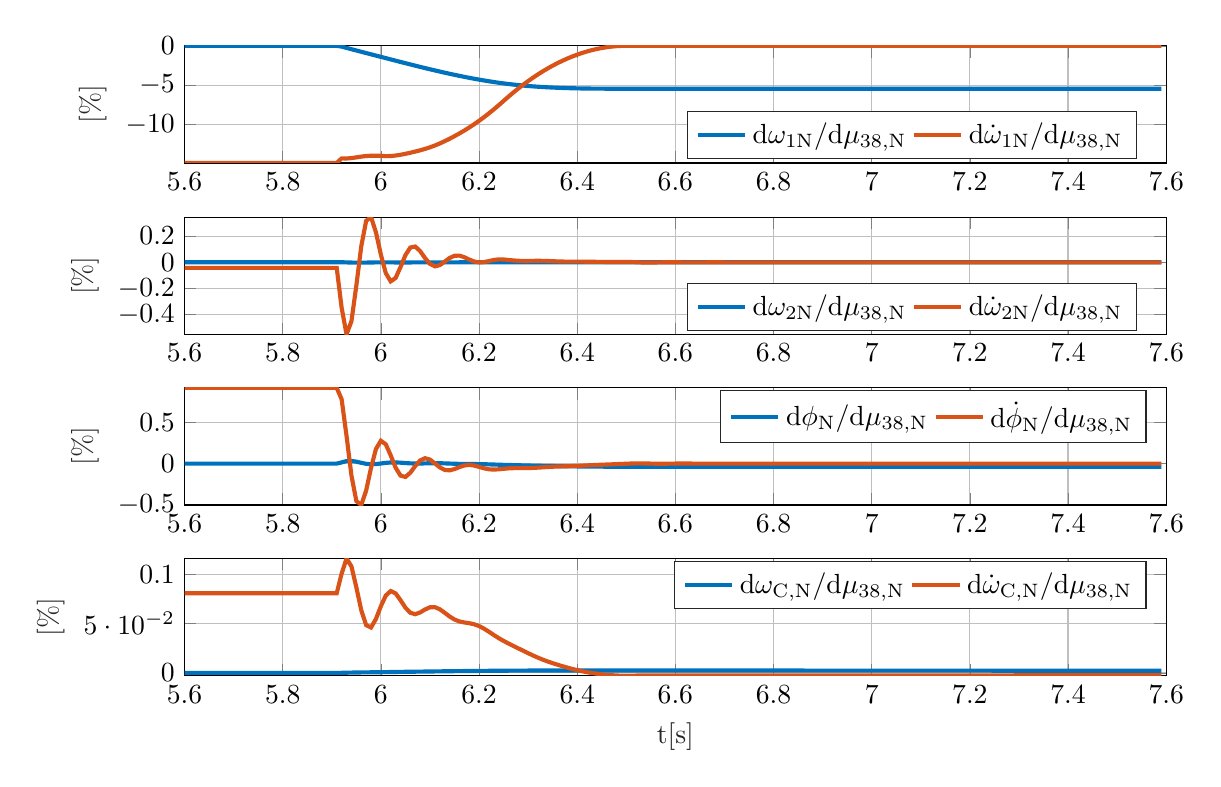
\begin{tikzpicture}

\begin{axis}[%
width=0.959\muwidth,
height=0.186\muheight,
at={(0\muwidth,0.814\muheight)},
scale only axis,
xmin=5.6,
xmax=7.6,
ymin=-14.8952327714782,
ymax=0.00043105236911729,
ylabel style={font=\color{white!15!black}},
ylabel={[$\%$]},
axis background/.style={fill=white},
xmajorgrids,
ymajorgrids,
legend style={at={(0.97,0.03)}, anchor=south east, legend columns=2, legend cell align=left, align=left, draw=white!15!black}
]
\addplot [color=mycolor1, line width=1.5pt]
  table[row sep=crcr]{%
5.59	0\\
5.6	0\\
5.61	0\\
5.62	0\\
5.63	0\\
5.64	0\\
5.65	0\\
5.66	0\\
5.67	0\\
5.68	0\\
5.69	0\\
5.7	0\\
5.71	0\\
5.72	0\\
5.73	0\\
5.74	0\\
5.75	0\\
5.76	0\\
5.77	0\\
5.78	0\\
5.79	0\\
5.8	0\\
5.81	0\\
5.82	0\\
5.83	0\\
5.84	0\\
5.85	0\\
5.86	0\\
5.87	0\\
5.88	0\\
5.89	0\\
5.9	0\\
5.91	0\\
5.92	-0.0998884187134601\\
5.93	-0.265336622808697\\
5.94	-0.430534967135716\\
5.95	-0.594891332713016\\
5.96	-0.758131145275483\\
5.97	-0.920357450527906\\
5.98	-1.08194046960611\\
5.99	-1.24331054487414\\
6	-1.40473387904871\\
6.01	-1.5663321056994\\
6.02	-1.72831971819269\\
6.03	-1.8898339140989\\
6.04	-2.05041016740977\\
6.05	-2.2097082136108\\
6.06	-2.36751880567463\\
6.07	-2.52368759410275\\
6.08	-2.67808265667713\\
6.09	-2.83052642115429\\
6.1	-2.98077119533476\\
6.11	-3.12850925718606\\
6.12	-3.27340767029095\\
6.13	-3.41514617172957\\
6.14	-3.55343546300558\\
6.15	-3.68803678890156\\
6.16	-3.81872693204366\\
6.17	-3.94528773407803\\
6.18	-4.06748085914056\\
6.19	-4.18504742962766\\
6.2	-4.2977242504695\\
6.21	-4.40523058872338\\
6.22	-4.50728168976378\\
6.23	-4.60360911644536\\
6.24	-4.693958146126\\
6.25	-4.77808231152816\\
6.26	-4.85571540620147\\
6.27	-4.92725165582361\\
6.28	-4.99283685046462\\
6.29	-5.05272150345875\\
6.3	-5.1071656284549\\
6.31	-5.15642449315845\\
6.32	-5.20075575359575\\
6.33	-5.24042133707204\\
6.34	-5.2756833151407\\
6.35	-5.30680260486082\\
6.36	-5.33403883150207\\
6.37	-5.35765052721081\\
6.38	-5.37789553228134\\
6.39	-5.39503167205322\\
6.4	-5.40931728090118\\
6.41	-5.42101139115916\\
6.42	-5.4303735764787\\
6.43	-5.43766359047922\\
6.44	-5.44314101197473\\
6.45	-5.4470650407414\\
6.46	-5.44969450519555\\
6.47	-5.45128803136421\\
6.48	-5.45210426004205\\
6.49	-5.45240201234393\\
6.5	-5.45244028738861\\
6.51	-5.45243585363191\\
6.52	-5.45243439024478\\
6.53	-5.45243708435664\\
6.54	-5.45244312530129\\
6.55	-5.4524504289252\\
6.56	-5.45245682733422\\
6.57	-5.45246102574698\\
6.58	-5.45246296280448\\
6.59	-5.45246357884296\\
6.6	-5.45246416448677\\
6.61	-5.45246574072393\\
6.62	-5.45246866157117\\
6.63	-5.45247262030438\\
6.64	-5.45247693075185\\
6.65	-5.45248092143005\\
6.66	-5.452484197369\\
6.67	-5.45248675487514\\
6.68	-5.45248889773135\\
6.69	-5.45249104640071\\
6.7	-5.4524935230667\\
6.71	-5.45249643638983\\
6.72	-5.45249967716771\\
6.73	-5.45250301922714\\
6.74	-5.45250624249174\\
6.75	-5.45250922565268\\
6.76	-5.45251197765917\\
6.77	-5.4525146080901\\
6.78	-5.45251724632836\\
6.79	-5.45251999269\\
6.8	-5.45252287608518\\
6.81	-5.45252585145331\\
6.82	-5.45252885364579\\
6.83	-5.45253181511517\\
6.84	-5.45253469974614\\
6.85	-5.45253751165447\\
6.86	-5.45254028431447\\
6.87	-5.45254305938912\\
6.88	-5.45254586694511\\
6.89	-5.45254871504186\\
6.9	-5.45255159123876\\
6.91	-5.45255447259646\\
6.92	-5.45255733799123\\
6.93	-5.45256017681365\\
6.94	-5.45256299124743\\
6.95	-5.45256579237491\\
6.96	-5.45256859345866\\
6.97	-5.45257140370718\\
6.98	-5.45257422512697\\
6.99	-5.45257705334672\\
7	-5.45257988104848\\
7.01	-5.45258270164196\\
7.02	-5.45258551218056\\
7.03	-5.45258831393585\\
7.04	-5.45259111021163\\
7.05	-5.45259390510381\\
7.06	-5.45259670123669\\
7.07	-5.452599499095\\
7.08	-5.45260229719272\\
7.09	-5.45260509325207\\
7.1	-5.45260788540684\\
7.11	-5.45261067279773\\
7.12	-5.45261345571798\\
7.13	-5.45261623547096\\
7.14	-5.45261901317411\\
7.15	-5.45262178961957\\
7.16	-5.45262456491068\\
7.17	-5.45262733860082\\
7.18	-5.45263010992945\\
7.19	-5.45263287838505\\
7.2	-5.45263564370082\\
7.21	-5.45263840600347\\
7.22	-5.45264116560118\\
7.23	-5.45264392300971\\
7.24	-5.45264667838716\\
7.25	-5.45264943175223\\
7.26	-5.45265218287761\\
7.27	-5.45265493154868\\
7.28	-5.45265767776028\\
7.29	-5.45266042137798\\
7.3	-5.45266316241159\\
7.31	-5.45266590097583\\
7.32	-5.45266863708483\\
7.33	-5.4526713710361\\
7.34	-5.45267410272383\\
7.35	-5.45267683202162\\
7.36	-5.45267955880421\\
7.37	-5.45268228319527\\
7.38	-5.45268500527389\\
7.39	-5.45268772491606\\
7.4	-5.45269044215313\\
7.41	-5.45269315702308\\
7.42	-5.45269586940362\\
7.43	-5.45269857958438\\
7.44	-5.45270128741621\\
7.45	-5.45270399287451\\
7.46	-5.45270669575971\\
7.47	-5.45270939629249\\
7.48	-5.45271209454765\\
7.49	-5.45271479030178\\
7.5	-5.45271748352572\\
7.51	-5.45272017470521\\
7.52	-5.45272286309103\\
7.53	-5.45272554931452\\
7.54	-5.45272823317574\\
7.55	-5.45273091475728\\
7.56	-5.45273359412853\\
7.57	-5.45273627101989\\
7.58	-5.4527389456755\\
7.59	-5.45274161797718\\
};
\addlegendentry{d$\omega_{1\mathrm{N}}/$d$\mu_\mathrm{38,N}$}

\addplot [color=mycolor2, line width=1.5pt]
  table[row sep=crcr]{%
5.59	-14.8952327714782\\
5.6	-14.8952327714782\\
5.61	-14.8952327714782\\
5.62	-14.8952327714782\\
5.63	-14.8952327714782\\
5.64	-14.8952327714782\\
5.65	-14.8952327714782\\
5.66	-14.8952327714782\\
5.67	-14.8952327714782\\
5.68	-14.8952327714782\\
5.69	-14.8952327714782\\
5.7	-14.8952327714782\\
5.71	-14.8952327714782\\
5.72	-14.8952327714782\\
5.73	-14.8952327714782\\
5.74	-14.8952327714782\\
5.75	-14.8952327714782\\
5.76	-14.8952327714782\\
5.77	-14.8952327714782\\
5.78	-14.8952327714782\\
5.79	-14.8952327714782\\
5.8	-14.8952327714782\\
5.81	-14.8952327714782\\
5.82	-14.8952327714782\\
5.83	-14.8952327714782\\
5.84	-14.8952327714782\\
5.85	-14.8952327714782\\
5.86	-14.8952327714782\\
5.87	-14.8952327714782\\
5.88	-14.8952327714782\\
5.89	-14.8952327714782\\
5.9	-14.8952327714782\\
5.91	-14.8952327714782\\
5.92	-14.309232443867\\
5.93	-14.3256418736507\\
5.94	-14.2732521430176\\
5.95	-14.1814992130989\\
5.96	-14.0838844449375\\
5.97	-14.0098687680649\\
5.98	-13.9737479591872\\
5.99	-13.9705028220729\\
6	-13.979312364013\\
6.01	-14.0297440486181\\
6.02	-14.0103520100497\\
6.03	-13.9483957804268\\
6.04	-13.8509755100101\\
6.05	-13.7293462230979\\
6.06	-13.5927366846033\\
6.07	-13.445200235602\\
6.08	-13.2849210212748\\
6.09	-13.106306761787\\
6.1	-12.9032577371184\\
6.11	-12.6718990965597\\
6.12	-12.411787896604\\
6.13	-12.1253215510072\\
6.14	-11.8161012963566\\
6.15	-11.4869055732983\\
6.16	-11.1389273488609\\
6.17	-10.7715489495381\\
6.18	-10.3829593290929\\
6.19	-9.97126121951027\\
6.2	-9.53532016429004\\
6.21	-9.07491468959758\\
6.22	-8.59078500409343\\
6.23	-8.08408490879371\\
6.24	-7.55579432961754\\
6.25	-7.0062943779019\\
6.26	-6.45748675476932\\
6.27	-5.93110173592127\\
6.28	-5.42690459600135\\
6.29	-4.94479803803532\\
6.3	-4.48484676190753\\
6.31	-4.04721731919213\\
6.32	-3.63208396594935\\
6.33	-3.23955314399768\\
6.34	-2.86963249937315\\
6.35	-2.52224580984919\\
6.36	-2.19728543901414\\
6.37	-1.89466693376357\\
6.38	-1.61436034973303\\
6.39	-1.35639126854202\\
6.4	-1.1208175513172\\
6.41	-0.907696766827801\\
6.42	-0.7170613608461\\
6.43	-0.548910008854944\\
6.44	-0.403215611085122\\
6.45	-0.279942925641865\\
6.46	-0.179065604720064\\
6.47	-0.10057578593353\\
6.48	-0.0444834381488791\\
6.49	-0.0108080248908367\\
6.5	0.00043105236911729\\
6.51	0.000290109063843299\\
6.52	-5.20535810922849e-05\\
6.53	-0.000403194565271111\\
6.54	-0.000612786970029975\\
6.55	-0.000620130694488269\\
6.56	-0.000468139304263234\\
6.57	-0.000257407408449133\\
6.58	-9.23243964588785e-05\\
6.59	-3.39420585395693e-05\\
6.6	-8.33300651547874e-05\\
6.61	-0.000195193810353125\\
6.62	-0.000307009230731904\\
6.63	-0.000369869837053347\\
6.64	-0.000368561836736334\\
6.65	-0.000317629296223657\\
6.66	-0.000249726814808404\\
6.67	-0.000197445634325016\\
6.68	-0.00017994116200028\\
6.69	-0.000197046506822042\\
6.7	-0.000233574427654432\\
6.71	-0.000269164640183645\\
6.72	-0.000288519003010278\\
6.73	-0.00028680338905336\\
6.74	-0.000269404132329282\\
6.75	-0.000247249097688012\\
6.76	-0.00023105861535451\\
6.77	-0.000226111613272577\\
6.78	-0.000231926258950046\\
6.79	-0.000243538384533659\\
6.8	-0.000254262866548018\\
6.81	-0.000259853005153089\\
6.82	-0.000258949599763991\\
6.83	-0.000253277959140218\\
6.84	-0.000246256575255175\\
6.85	-0.000241127150207235\\
6.86	-0.000239575486022866\\
6.87	-0.000241363339193761\\
6.88	-0.000244862669441243\\
6.89	-0.000248073455417504\\
6.9	-0.000249572802145731\\
6.91	-0.000248999673483501\\
6.92	-0.000246971085601362\\
6.93	-0.000244593103461845\\
6.94	-0.000242878313169892\\
6.95	-0.000242322124502779\\
6.96	-0.000242807998841115\\
6.97	-0.000243794869806225\\
6.98	-0.000244645084247157\\
6.99	-0.000244931986098331\\
7	-0.000244572861217444\\
7.01	-0.000243776062804243\\
7.02	-0.000242905046283331\\
7.03	-0.000242255349171547\\
7.04	-0.000241965673907478\\
7.05	-0.000241990205018306\\
7.06	-0.000242151048601469\\
7.07	-0.000242256188640093\\
7.08	-0.000242185373231313\\
7.09	-0.000241914809277053\\
7.1	-0.000241520294778146\\
7.11	-0.000241106356128541\\
7.12	-0.000240769377977271\\
7.13	-0.000240543266416697\\
7.14	-0.000240412311607005\\
7.15	-0.000240320469815337\\
7.16	-0.000240205557118105\\
7.17	-0.000240034850127773\\
7.18	-0.000239803581247105\\
7.19	-0.000239535919751112\\
7.2	-0.000239264551691957\\
7.21	-0.000239017531612912\\
7.22	-0.000238807433014154\\
7.23	-0.000238624693236054\\
7.24	-0.000238453649771756\\
7.25	-0.000238275433252443\\
7.26	-0.000238077881292242\\
7.27	-0.000237861388744779\\
7.28	-0.00023763477323862\\
7.29	-0.000237407600050745\\
7.3	-0.000237188283833724\\
7.31	-0.00023698060188089\\
7.32	-0.000236782186584626\\
7.33	-0.000236586705477512\\
7.34	-0.000236388945146688\\
7.35	-0.000236185248622479\\
7.36	-0.000235975609712092\\
7.37	-0.000235763096405897\\
7.38	-0.000235550670931257\\
7.39	-0.000235340675423718\\
7.4	-0.000235134207623694\\
7.41	-0.000234930618778465\\
7.42	-0.000234728168980333\\
7.43	-0.000234525113102693\\
7.44	-0.000234320480788933\\
7.45	-0.000234114142382395\\
7.46	-0.000233906792418186\\
7.47	-0.00023369958055444\\
7.48	-0.000233493187097009\\
7.49	-0.000233287963872428\\
7.5	-0.000233083682228151\\
7.51	-0.000232879758737928\\
7.52	-0.000232675800856054\\
7.53	-0.000232471546268633\\
7.54	-0.000232266964200653\\
7.55	-0.000232062216703801\\
7.56	-0.000231857503191161\\
7.57	-0.000231653034135445\\
7.58	-0.000231448895119255\\
7.59	-0.000231245092780559\\
};
\addlegendentry{d$\dot{\omega}_{1\mathrm{N}}/$d$\mu_\mathrm{38,N}$}

\end{axis}

\begin{axis}[%
width=0.959\muwidth,
height=0.186\muheight,
at={(0\muwidth,0.542\muheight)},
scale only axis,
xmin=5.6,
xmax=7.6,
ymin=-0.551982004409516,
ymax=0.34475292796271,
ylabel style={font=\color{white!15!black}},
ylabel={[$\%$]},
axis background/.style={fill=white},
xmajorgrids,
ymajorgrids,
legend style={at={(0.97,0.03)}, anchor=south east, legend columns=2, legend cell align=left, align=left, draw=white!15!black}
]
\addplot [color=mycolor1, line width=1.5pt]
  table[row sep=crcr]{%
5.59	0\\
5.6	0\\
5.61	0\\
5.62	0\\
5.63	0\\
5.64	0\\
5.65	0\\
5.66	0\\
5.67	0\\
5.68	0\\
5.69	0\\
5.7	0\\
5.71	0\\
5.72	0\\
5.73	0\\
5.74	0\\
5.75	0\\
5.76	0\\
5.77	0\\
5.78	0\\
5.79	0\\
5.8	0\\
5.81	0\\
5.82	0\\
5.83	0\\
5.84	0\\
5.85	0\\
5.86	0\\
5.87	0\\
5.88	0\\
5.89	0\\
5.9	0\\
5.91	0\\
5.92	-0.000339242484012616\\
5.93	-0.00151072160217907\\
5.94	-0.00278298101197889\\
5.95	-0.00357396057503692\\
5.96	-0.00363685280310564\\
5.97	-0.00307035136249888\\
5.98	-0.00222243368982364\\
5.99	-0.00151314332814877\\
6	-0.00116456640051768\\
6.01	-0.00121247024828596\\
6.02	-0.00151466385740764\\
6.03	-0.00185919938338354\\
6.04	-0.00205834547278001\\
6.05	-0.0020325757987805\\
6.06	-0.00181825858909758\\
6.07	-0.00152203456346705\\
6.08	-0.00126371947570767\\
6.09	-0.00111998990380292\\
6.1	-0.00110161613597874\\
6.11	-0.00116294487049464\\
6.12	-0.00123462313800076\\
6.13	-0.00125921012427926\\
6.14	-0.0012137292845424\\
6.15	-0.00111120442399594\\
6.16	-0.000986197050311071\\
6.17	-0.000875979959616679\\
6.18	-0.000804411357219596\\
6.19	-0.000773690734139497\\
6.2	-0.000770206559999477\\
6.21	-0.000772859373260719\\
6.22	-0.000762539077650412\\
6.23	-0.00073097458785576\\
6.24	-0.000682629763921056\\
6.25	-0.000629354030778545\\
6.26	-0.000582763673989806\\
6.27	-0.000545444176064616\\
6.28	-0.000516033097557186\\
6.29	-0.000491289352802265\\
6.3	-0.000467651789731487\\
6.31	-0.000442955031606843\\
6.32	-0.000416925259787925\\
6.33	-0.000390869449307579\\
6.34	-0.000366716546215787\\
6.35	-0.000346021540122742\\
6.36	-0.000329283034175645\\
6.37	-0.000315911430148452\\
6.38	-0.000304673664008918\\
6.39	-0.000294324560892823\\
6.4	-0.000284096556011066\\
6.41	-0.000273878198722299\\
6.42	-0.00026406686736462\\
6.43	-0.000255229085458123\\
6.44	-0.00024776707324281\\
6.45	-0.000241726783663656\\
6.46	-0.000236805118626235\\
6.47	-0.000232508748959767\\
6.48	-0.000228358226026294\\
6.49	-0.000224043588896622\\
6.5	-0.000219470123626315\\
6.51	-0.000215302718617577\\
6.52	-0.000213927242404314\\
6.53	-0.000216459509298669\\
6.54	-0.000222137552708516\\
6.55	-0.00022900242171223\\
6.56	-0.000235016455326482\\
6.57	-0.000238962654360345\\
6.58	-0.000240783345864366\\
6.59	-0.000241362376700464\\
6.6	-0.000241912838780006\\
6.61	-0.000243394385718869\\
6.62	-0.000246139767169964\\
6.63	-0.000249860685062335\\
6.64	-0.0002539121884795\\
6.65	-0.000257663132312601\\
6.66	-0.000260742273847902\\
6.67	-0.000263146141414704\\
6.68	-0.000265160268554372\\
6.69	-0.000267179859630148\\
6.7	-0.00026950774339787\\
6.71	-0.00027224605274837\\
6.72	-0.000275292145464099\\
6.73	-0.000278433435386985\\
6.74	-0.000281463066913518\\
6.75	-0.000284267018668053\\
6.76	-0.000286853702251994\\
6.77	-0.00028932611375293\\
6.78	-0.000291805863560125\\
6.79	-0.000294387241404856\\
6.8	-0.000297097420683032\\
6.81	-0.000299894047766633\\
6.82	-0.00030271588776114\\
6.83	-0.000305499451048725\\
6.84	-0.000308210791877857\\
6.85	-0.00031085377877931\\
6.86	-0.000313459875138571\\
6.87	-0.000316068241091219\\
6.88	-0.000318707137116322\\
6.89	-0.000321384138470681\\
6.9	-0.000324087551896622\\
6.91	-0.000326795816086067\\
6.92	-0.000329489076306077\\
6.93	-0.000332157360475597\\
6.94	-0.000334802721115603\\
6.95	-0.000337435574808565\\
6.96	-0.000340068387403695\\
6.97	-0.000342709814208356\\
6.98	-0.000345361741183979\\
6.99	-0.000348020059620438\\
7	-0.000350677891180393\\
7.01	-0.000353329041486382\\
7.02	-0.000355970740941686\\
7.03	-0.000358604184734158\\
7.04	-0.000361232478185581\\
7.05	-0.000363859471155914\\
7.06	-0.000366487630297793\\
7.07	-0.000369117411212661\\
7.08	-0.00037174741715602\\
7.09	-0.00037437550718155\\
7.1	-0.000376999927191775\\
7.11	-0.00037961986949939\\
7.12	-0.000382235609735315\\
7.13	-0.000384848372977962\\
7.14	-0.000387459209528759\\
7.15	-0.000390068863939518\\
7.16	-0.00039267743334435\\
7.17	-0.00039528449796175\\
7.18	-0.000397889342929716\\
7.19	-0.000400491487464811\\
7.2	-0.000403090680788077\\
7.21	-0.000405687042001781\\
7.22	-0.000408280860766287\\
7.23	-0.00041087262186455\\
7.24	-0.00041346247390773\\
7.25	-0.000416050434447795\\
7.26	-0.000418636289851264\\
7.27	-0.000421219838382791\\
7.28	-0.000423801075189406\\
7.29	-0.000426379873924921\\
7.3	-0.00042895624380951\\
7.31	-0.000431530292666882\\
7.32	-0.000434102033774911\\
7.33	-0.000436671746770433\\
7.34	-0.000439239332214248\\
7.35	-0.00044180467128708\\
7.36	-0.000444367646256507\\
7.37	-0.000446928373365836\\
7.38	-0.000449486926948396\\
7.39	-0.000452043190449048\\
7.4	-0.000454597193330108\\
7.41	-0.000457148971302084\\
7.42	-0.000459698409398335\\
7.43	-0.000462245779872134\\
7.44	-0.000464790942524007\\
7.45	-0.000467333874225713\\
7.46	-0.000469874387411427\\
7.47	-0.000472412689487351\\
7.48	-0.000474948850772114\\
7.49	-0.000477482661273001\\
7.5	-0.00048001409358112\\
7.51	-0.000482543604260904\\
7.52	-0.000485070489088701\\
7.53	-0.000487595341495776\\
7.54	-0.000490117973540732\\
7.55	-0.000492638462844629\\
7.56	-0.000495156874638698\\
7.57	-0.000497672955528885\\
7.58	-0.000500186934974629\\
7.59	-0.000502698701899973\\
};
\addlegendentry{d$\omega_{2\mathrm{N}}/$d$\mu_\mathrm{38,N}$}

\addplot [color=mycolor2, line width=1.5pt]
  table[row sep=crcr]{%
5.59	-0.0434744990959547\\
5.6	-0.0434744990959547\\
5.61	-0.0434744990959547\\
5.62	-0.0434744990959547\\
5.63	-0.0434744990959547\\
5.64	-0.0434744990959547\\
5.65	-0.0434744990959547\\
5.66	-0.0434744990959547\\
5.67	-0.0434744990959547\\
5.68	-0.0434744990959547\\
5.69	-0.0434744990959547\\
5.7	-0.0434744990959547\\
5.71	-0.0434744990959547\\
5.72	-0.0434744990959547\\
5.73	-0.0434744990959547\\
5.74	-0.0434744990959547\\
5.75	-0.0434744990959547\\
5.76	-0.0434744990959547\\
5.77	-0.0434744990959547\\
5.78	-0.0434744990959547\\
5.79	-0.0434744990959547\\
5.8	-0.0434744990959547\\
5.81	-0.0434744990959547\\
5.82	-0.0434744990959547\\
5.83	-0.0434744990959547\\
5.84	-0.0434744990959547\\
5.85	-0.0434744990959547\\
5.86	-0.0434744990959547\\
5.87	-0.0434744990959547\\
5.88	-0.0434744990959547\\
5.89	-0.0434744990959547\\
5.9	-0.0434744990959547\\
5.91	-0.0434744990959547\\
5.92	-0.348025142073928\\
5.93	-0.551982004409516\\
5.94	-0.452084435717824\\
5.95	-0.178337615816037\\
5.96	0.121298263097482\\
5.97	0.316707747199332\\
5.98	0.34475292796271\\
5.99	0.227601299960349\\
6	0.0572096669474608\\
6.01	-0.0835832468721097\\
6.02	-0.146566897295886\\
6.03	-0.12065025773415\\
6.04	-0.0371914451268456\\
6.05	0.0541012449067317\\
6.06	0.112468577882435\\
6.07	0.120008799783952\\
6.08	0.0847417109922569\\
6.09	0.0313658542947585\\
6.1	-0.0131790962637468\\
6.11	-0.0317796969950671\\
6.12	-0.022479668978946\\
6.13	0.00413270751635172\\
6.14	0.0321524172602511\\
6.15	0.0493083584475312\\
6.16	0.050331741233249\\
6.17	0.0379505470440404\\
6.18	0.0201633389528184\\
6.19	0.00534948219731071\\
6.2	-0.00148064762604831\\
6.21	0.000651098134382051\\
6.22	0.00847555630820838\\
6.23	0.0168969154180871\\
6.24	0.0215872907808943\\
6.25	0.0208634878959433\\
6.26	0.0170819862468373\\
6.27	0.0133563730149219\\
6.28	0.0107233227645228\\
6.29	0.00961255173862755\\
6.3	0.00973831013391813\\
6.31	0.0103650158079697\\
6.32	0.0107230594273329\\
6.33	0.0103423361532053\\
6.34	0.00918907694085952\\
6.35	0.00759992050990948\\
6.36	0.00605024767090469\\
6.37	0.00491304916713047\\
6.38	0.00432057556346345\\
6.39	0.00415984454440408\\
6.4	0.0041753099725355\\
6.41	0.00411271691906788\\
6.42	0.00382876724473718\\
6.43	0.00332931073611847\\
6.44	0.00273403468156263\\
6.45	0.002198586414934\\
6.46	0.0018393321429981\\
6.47	0.00169099643022925\\
6.48	0.00170955135133162\\
6.49	0.00180903541794249\\
6.5	0.00190376120242627\\
6.51	0.00128127907369604\\
6.52	-0.000229896864582298\\
6.53	-0.00178072602167605\\
6.54	-0.00270639983091708\\
6.55	-0.00273883370370528\\
6.56	-0.00206755723582325\\
6.57	-0.00113685081565861\\
6.58	-0.000407754640986586\\
6.59	-0.000149906551518183\\
6.6	-0.000368030792551303\\
6.61	-0.000862081801951371\\
6.62	-0.00135591938272151\\
6.63	-0.00163354593589606\\
6.64	-0.00162776909661921\\
6.65	-0.00140282335564668\\
6.66	-0.00110292914573537\\
6.67	-0.000872027078719405\\
6.68	-0.000794717828919833\\
6.69	-0.000870264315052119\\
6.7	-0.00103159143785251\\
6.71	-0.00118877713187374\\
6.72	-0.00127425650210085\\
6.73	-0.00126667941977046\\
6.74	-0.00118983485916592\\
6.75	-0.00109198620222699\\
6.76	-0.00102048024535636\\
6.77	-0.000998631599329504\\
6.78	-0.00102431223036111\\
6.79	-0.00107559767906204\\
6.8	-0.00112296281201995\\
6.81	-0.00114765189797561\\
6.82	-0.00114366196948186\\
6.83	-0.00111861292637893\\
6.84	-0.00108760268450265\\
6.85	-0.00106494835965335\\
6.86	-0.00105809536849724\\
6.87	-0.00106599149840215\\
6.88	-0.00108144643992882\\
6.89	-0.00109562701335528\\
6.9	-0.00110224894223136\\
6.91	-0.00109971769501107\\
6.92	-0.00109075834996992\\
6.93	-0.00108025589026515\\
6.94	-0.00107268244568629\\
6.95	-0.00107022601467801\\
6.96	-0.00107237189944944\\
6.97	-0.00107673045722521\\
6.98	-0.00108048546562408\\
6.99	-0.001081752579906\\
7	-0.001080166489528\\
7.01	-0.00107664739529754\\
7.02	-0.00107280051362377\\
7.03	-0.00106993109857501\\
7.04	-0.00106865173539657\\
7.05	-0.00106876007809547\\
7.06	-0.00106947045065163\\
7.07	-0.00106993480612372\\
7.08	-0.00106962204684567\\
7.09	-0.00106842708958338\\
7.1	-0.00106668469944565\\
7.11	-0.00106485652171649\\
7.12	-0.00106336824331601\\
7.13	-0.00106236961194939\\
7.14	-0.00106179124443811\\
7.15	-0.00106138562124179\\
7.16	-0.00106087810440549\\
7.17	-0.00106012416969023\\
7.18	-0.00105910276079913\\
7.19	-0.00105792062236776\\
7.2	-0.0010567221137419\\
7.21	-0.00105563113901025\\
7.22	-0.00105470322957361\\
7.23	-0.00105389615153718\\
7.24	-0.00105314073077022\\
7.25	-0.00105235362989941\\
7.26	-0.00105148113322796\\
7.27	-0.00105052498464366\\
7.28	-0.00104952412757991\\
7.29	-0.00104852080749099\\
7.3	-0.00104755218804947\\
7.31	-0.00104663495183278\\
7.32	-0.00104575864220069\\
7.33	-0.0010448952915403\\
7.34	-0.00104402187459106\\
7.35	-0.00104312224019016\\
7.36	-0.00104219636098678\\
7.37	-0.00104125778689155\\
7.38	-0.00104031960070818\\
7.39	-0.00103939214657828\\
7.4	-0.00103848027271934\\
7.41	-0.00103758111388719\\
7.42	-0.00103668698570531\\
7.43	-0.00103579018074733\\
7.44	-0.00103488641339185\\
7.45	-0.00103397511100473\\
7.46	-0.00103305934103001\\
7.47	-0.0010321441809818\\
7.48	-0.00103123263546012\\
7.49	-0.00103032625832181\\
7.5	-0.00102942403971306\\
7.51	-0.00102852340290707\\
7.52	-0.00102762261420884\\
7.53	-0.00102672051509791\\
7.54	-0.0010258169696551\\
7.55	-0.00102491269358858\\
7.56	-0.00102400856761483\\
7.57	-0.00102310552129548\\
7.58	-0.00102220393260982\\
7.59	-0.0010213038308747\\
};
\addlegendentry{d$\dot{\omega}_{2\mathrm{N}}/$d$\mu_\mathrm{38,N}$}

\end{axis}

\begin{axis}[%
width=0.959\muwidth,
height=0.186\muheight,
at={(0\muwidth,0.271\muheight)},
scale only axis,
xmin=5.6,
xmax=7.6,
ymin=-0.50223080392396,
ymax=0.918114322144536,
ylabel style={font=\color{white!15!black}},
ylabel={[$\%$]},
axis background/.style={fill=white},
xmajorgrids,
ymajorgrids,
legend style={legend columns=2, legend cell align=left, align=left, draw=white!15!black}
]
\addplot [color=mycolor1, line width=1.5pt]
  table[row sep=crcr]{%
5.59	0\\
5.6	0\\
5.61	0\\
5.62	0\\
5.63	0\\
5.64	0\\
5.65	0\\
5.66	0\\
5.67	0\\
5.68	0\\
5.69	0\\
5.7	0\\
5.71	0\\
5.72	0\\
5.73	0\\
5.74	0\\
5.75	0\\
5.76	0\\
5.77	0\\
5.78	0\\
5.79	0\\
5.8	0\\
5.81	0\\
5.82	0\\
5.83	0\\
5.84	0\\
5.85	0\\
5.86	0\\
5.87	0\\
5.88	0\\
5.89	0\\
5.9	0\\
5.91	0\\
5.92	0.0145330713029577\\
5.93	0.030590943426906\\
5.94	0.0324359376659837\\
5.95	0.0234334198199662\\
5.96	0.00950743249763991\\
5.97	-0.00254172148729018\\
5.98	-0.00790236064608305\\
5.99	-0.00553216838627695\\
6	0.00123325624488847\\
6.01	0.00872046633225194\\
6.02	0.0135475862708431\\
6.03	0.0142060717293497\\
6.04	0.0112685672761549\\
6.05	0.0067418137365591\\
6.06	0.00278294484915517\\
6.07	0.000795815485103172\\
6.08	0.000994982439859793\\
6.09	0.00256970953078451\\
6.1	0.00426865429853395\\
6.11	0.00503221250821767\\
6.12	0.00441562639672986\\
6.13	0.00264183966631995\\
6.14	0.000364972254122595\\
6.15	-0.00175548969800989\\
6.16	-0.00329077480529026\\
6.17	-0.00418582785322239\\
6.18	-0.00470850878479459\\
6.19	-0.00525423662641614\\
6.2	-0.00613485771400261\\
6.21	-0.00750463399105496\\
6.22	-0.0093020685998007\\
6.23	-0.0113225585688624\\
6.24	-0.0133345402116704\\
6.25	-0.0151973538928258\\
6.26	-0.016893402728026\\
6.27	-0.0184857240868786\\
6.28	-0.0200310526890784\\
6.29	-0.0215659393048472\\
6.3	-0.0230938660751977\\
6.31	-0.0245895074576233\\
6.32	-0.0260163594888708\\
6.33	-0.0273444573129076\\
6.34	-0.0285618414612572\\
6.35	-0.0296763822935873\\
6.36	-0.0307079943537501\\
6.37	-0.0316771151329223\\
6.38	-0.0325957626411258\\
6.39	-0.0334641369337772\\
6.4	-0.0342731263714152\\
6.41	-0.0350103769552001\\
6.42	-0.0356663468107813\\
6.43	-0.0362378676024161\\
6.44	-0.0367281139646886\\
6.45	-0.0371437980723363\\
6.46	-0.0374914884403322\\
6.47	-0.0377747577331596\\
6.48	-0.0379932943946058\\
6.49	-0.0381439022702317\\
6.5	-0.0382223147852798\\
6.51	-0.0382271003164417\\
6.52	-0.038174757695447\\
6.53	-0.0381007947383073\\
6.54	-0.0380412397016848\\
6.55	-0.038018979204222\\
6.56	-0.0380350826026961\\
6.57	-0.0380741592141127\\
6.58	-0.0381141657282815\\
6.59	-0.0381375873260393\\
6.6	-0.0381380834210828\\
6.61	-0.0381205097722579\\
6.62	-0.0380965667268329\\
6.63	-0.0380781700828421\\
6.64	-0.038071824034068\\
6.65	-0.0380775966122448\\
6.66	-0.0380903717421896\\
6.67	-0.0381031940431115\\
6.68	-0.0381105266586553\\
6.69	-0.0381104141511466\\
6.7	-0.0381045800404966\\
6.71	-0.0380968657277704\\
6.72	-0.0380910612583562\\
6.73	-0.0380892718395731\\
6.74	-0.0380913871700568\\
6.75	-0.0380956436474944\\
6.76	-0.0380997051142989\\
6.77	-0.0381019234482406\\
6.78	-0.0381017888669129\\
6.79	-0.0380998881268695\\
6.8	-0.0380975145308563\\
6.81	-0.0380957908480606\\
6.82	-0.0380953160264831\\
6.83	-0.0380960408691361\\
6.84	-0.038097405139875\\
6.85	-0.038098695910764\\
6.86	-0.0380993940974869\\
6.87	-0.038099353471517\\
6.88	-0.0380987800542573\\
6.89	-0.0380980636647239\\
6.9	-0.0380975677271095\\
6.91	-0.0380974782040008\\
6.92	-0.0380977632107581\\
6.93	-0.0380982364419616\\
6.94	-0.038098671008228\\
6.95	-0.038098908526662\\
6.96	-0.0380989112123288\\
6.97	-0.0380987512809286\\
6.98	-0.0380985557665273\\
6.99	-0.0380984368758559\\
7	-0.0380984472333771\\
7.01	-0.0380985734270334\\
7.02	-0.0380987517565915\\
7.03	-0.038098913220519\\
7.04	-0.0380990121577699\\
7.05	-0.038099038712106\\
7.06	-0.0380990187132526\\
7.07	-0.0380989905670886\\
7.08	-0.0380989875371322\\
7.09	-0.0380990252139877\\
7.1	-0.03809909657934\\
7.11	-0.0380991832568422\\
7.12	-0.0380992630554152\\
7.13	-0.0380993229343133\\
7.14	-0.0380993607259191\\
7.15	-0.0380993842393308\\
7.16	-0.0380994066676608\\
7.17	-0.0380994374363443\\
7.18	-0.0380994807654083\\
7.19	-0.0380995342031527\\
7.2	-0.0380995918987233\\
7.21	-0.0380996472663632\\
7.22	-0.0380996958660085\\
7.23	-0.038099737903724\\
7.24	-0.0380997756720309\\
7.25	-0.0380998130520799\\
7.26	-0.0380998534123933\\
7.27	-0.0380998978257399\\
7.28	-0.0380999451734424\\
7.29	-0.038099993708227\\
7.3	-0.0381000414493594\\
7.31	-0.0381000870583968\\
7.32	-0.0381001304127684\\
7.33	-0.038100172586067\\
7.34	-0.0381002146593342\\
7.35	-0.0381002576468199\\
7.36	-0.0381003019193134\\
7.37	-0.0381003470612596\\
7.38	-0.0381003924954711\\
7.39	-0.0381004376771506\\
7.4	-0.0381004822114815\\
7.41	-0.038100526063723\\
7.42	-0.0381005694874426\\
7.43	-0.0381006128759628\\
7.44	-0.0381006564916768\\
7.45	-0.0381007004608189\\
7.46	-0.0381007447278745\\
7.47	-0.0381007890665151\\
7.48	-0.0381008333053366\\
7.49	-0.0381008773275383\\
7.5	-0.0381009211251194\\
7.51	-0.0381009648049309\\
7.52	-0.0381010084371232\\
7.53	-0.0381010521074138\\
7.54	-0.0381010958434743\\
7.55	-0.0381011396289348\\
7.56	-0.0381011834283583\\
7.57	-0.0381012271979353\\
7.58	-0.0381012709076108\\
7.59	-0.0381013145453106\\
};
\addlegendentry{d$\phi_\mathrm{N}/$d$\mu_\mathrm{38,N}$}

\addplot [color=mycolor2, line width=1.5pt]
  table[row sep=crcr]{%
5.59	0.918114322144536\\
5.6	0.918114322144536\\
5.61	0.918114322144536\\
5.62	0.918114322144536\\
5.63	0.918114322144536\\
5.64	0.918114322144536\\
5.65	0.918114322144536\\
5.66	0.918114322144536\\
5.67	0.918114322144536\\
5.68	0.918114322144536\\
5.69	0.918114322144536\\
5.7	0.918114322144536\\
5.71	0.918114322144536\\
5.72	0.918114322144536\\
5.73	0.918114322144536\\
5.74	0.918114322144536\\
5.75	0.918114322144536\\
5.76	0.918114322144536\\
5.77	0.918114322144536\\
5.78	0.918114322144536\\
5.79	0.918114322144536\\
5.8	0.918114322144536\\
5.81	0.918114322144536\\
5.82	0.918114322144536\\
5.83	0.918114322144536\\
5.84	0.918114322144536\\
5.85	0.918114322144536\\
5.86	0.918114322144536\\
5.87	0.918114322144536\\
5.88	0.918114322144536\\
5.89	0.918114322144536\\
5.9	0.918114322144536\\
5.91	0.918114322144536\\
5.92	0.780873596157841\\
5.93	0.336000289599134\\
5.94	-0.144758817987026\\
5.95	-0.453547858622582\\
5.96	-0.50223080392396\\
5.97	-0.326061399638654\\
5.98	-0.0493162472527121\\
5.99	0.178000333552247\\
6	0.276573165857691\\
6.01	0.233620742921505\\
6.02	0.0998679118876485\\
6.03	-0.0488890150406191\\
6.04	-0.145564727485664\\
6.05	-0.161720033341336\\
6.06	-0.110305800424417\\
6.07	-0.0293642652230558\\
6.08	0.0383571048308141\\
6.09	0.0655179987531124\\
6.1	0.0483152265752814\\
6.11	0.00309544603575382\\
6.12	-0.0453318128130518\\
6.13	-0.0764119963153649\\
6.14	-0.0818981901451405\\
6.15	-0.0664020204104818\\
6.16	-0.0422252909256064\\
6.17	-0.0226379930751332\\
6.18	-0.0161181709484889\\
6.19	-0.0234093410511228\\
6.2	-0.0396106813866658\\
6.21	-0.0571459824367309\\
6.22	-0.0691488272461693\\
6.23	-0.072624635434947\\
6.24	-0.0691268700226305\\
6.25	-0.0628465395089092\\
6.26	-0.0578879257454122\\
6.27	-0.0552392473755258\\
6.28	-0.0544385572031732\\
6.29	-0.0543704865723846\\
6.3	-0.0538069918081341\\
6.31	-0.0520174481962269\\
6.32	-0.0489467796057098\\
6.33	-0.0451048202764742\\
6.34	-0.0412233704126205\\
6.35	-0.0379004851984037\\
6.36	-0.0353568715191035\\
6.37	-0.0334245791198914\\
6.38	-0.0317058244390706\\
6.39	-0.0297984670666015\\
6.4	-0.027470897107237\\
6.41	-0.0247257756779417\\
6.42	-0.0217474282474938\\
6.43	-0.0187805318741637\\
6.44	-0.0160110329268617\\
6.45	-0.0134975962050765\\
6.46	-0.0111741861874197\\
6.47	-0.00890678908624508\\
6.48	-0.00656630647268971\\
6.49	-0.00408412527489415\\
6.5	-0.00146845109758016\\
6.51	0.00100825782080895\\
6.52	0.00248699360482367\\
6.53	0.00256931591964301\\
6.54	0.00152629326213463\\
6.55	5.97116113255418e-05\\
6.56	-0.00110381900785955\\
6.57	-0.00152970700173964\\
6.58	-0.00119738767738407\\
6.59	-0.00042252912419957\\
6.6	0.000361633237955316\\
6.61	0.000812386185784149\\
6.62	0.000810906459734771\\
6.63	0.000460161198064959\\
6.64	-9.52011768221331e-06\\
6.65	-0.000372746241694093\\
6.66	-0.000496949332046935\\
6.67	-0.000380903055010867\\
6.68	-0.000126589647919634\\
6.69	0.000124847122829265\\
6.7	0.000265257493179419\\
6.71	0.000258167365129911\\
6.72	0.000140232431883955\\
6.73	-1.26301865578638e-05\\
6.74	-0.000126552575238902\\
6.75	-0.000160822025862181\\
6.76	-0.000118459247979759\\
6.77	-3.62348677686287e-05\\
6.78	4.24075242226217e-05\\
6.79	8.3776304286598e-05\\
6.8	7.81647059595136e-05\\
6.81	4.07575889977597e-05\\
6.82	-6.60115973760005e-06\\
6.83	-4.12336526451499e-05\\
6.84	-5.10093697730216e-05\\
6.85	-3.73025872241022e-05\\
6.86	-1.13428999705016e-05\\
6.87	1.28910714852699e-05\\
6.88	2.53131943549865e-05\\
6.89	2.32246801417746e-05\\
6.9	1.08081606511733e-05\\
6.91	-4.22956809741936e-06\\
6.92	-1.47912850726126e-05\\
6.93	-1.73093167390973e-05\\
6.94	-1.25104746825765e-05\\
6.95	-4.10869627376306e-06\\
6.96	3.45023077853767e-06\\
6.97	7.07980543574828e-06\\
6.98	6.11457914019348e-06\\
6.99	2.03794253183325e-06\\
7	-2.67418245703768e-06\\
7.01	-5.81272950717587e-06\\
7.02	-6.38113962111196e-06\\
7.03	-4.7886530444528e-06\\
7.04	-2.16849102621268e-06\\
7.05	8.5862226113264e-08\\
7.06	1.1075087649446e-06\\
7.07	7.0685175953783e-07\\
7.08	-5.81883728453488e-07\\
7.09	-2.01438060309455e-06\\
7.1	-2.93861941410506e-06\\
7.11	-3.07202208637794e-06\\
7.12	-2.52589493712493e-06\\
7.13	-1.71043717119054e-06\\
7.14	-1.01755046325872e-06\\
7.15	-7.43614611894996e-07\\
7.16	-8.9647861315542e-07\\
7.17	-1.30428107182131e-06\\
7.18	-1.74018520276406e-06\\
7.19	-2.01144140948363e-06\\
7.2	-2.03709024941008e-06\\
7.21	-1.85850583616783e-06\\
7.22	-1.59974161407499e-06\\
7.23	-1.39121350634147e-06\\
7.24	-1.30794484275669e-06\\
7.25	-1.36098147507067e-06\\
7.26	-1.49599225104898e-06\\
7.27	-1.63094492463236e-06\\
7.28	-1.71141365573783e-06\\
7.29	-1.71619266897191e-06\\
7.3	-1.65807507040538e-06\\
7.31	-1.5746527371061e-06\\
7.32	-1.51052025663401e-06\\
7.33	-1.48561049626484e-06\\
7.34	-1.50235722224122e-06\\
7.35	-1.54432446516784e-06\\
7.36	-1.58532245239261e-06\\
7.37	-1.60828038023299e-06\\
7.38	-1.60918882980486e-06\\
7.39	-1.59114642917136e-06\\
7.4	-1.56549223013733e-06\\
7.41	-1.5445275596995e-06\\
7.42	-1.53666472954023e-06\\
7.43	-1.54048856774066e-06\\
7.44	-1.55211510695247e-06\\
7.45	-1.56456244906037e-06\\
7.46	-1.57123278278209e-06\\
7.47	-1.57073438344761e-06\\
7.48	-1.56490016052406e-06\\
7.49	-1.55667397632938e-06\\
7.5	-1.5500906272108e-06\\
7.51	-1.54642386963362e-06\\
7.52	-1.54665420195465e-06\\
7.53	-1.54868361197093e-06\\
7.54	-1.5510172887655e-06\\
7.55	-1.55235803114024e-06\\
7.56	-1.55219360472558e-06\\
7.57	-1.55043754358077e-06\\
7.58	-1.54792242254224e-06\\
7.59	-1.54540345095262e-06\\
};
\addlegendentry{d$\dot{\phi}_\mathrm{N}/$d$\mu_\mathrm{38,N}$}

\end{axis}

\begin{axis}[%
width=0.959\muwidth,
height=0.186\muheight,
at={(0\muwidth,0\muheight)},
scale only axis,
xmin=5.6,
xmax=7.6,
xlabel style={font=\color{white!15!black}},
xlabel={t[s]},
ymin=-0.00290332720547747,
ymax=0.116142197671229,
ylabel style={font=\color{white!15!black}},
ylabel={[$\%$]},
axis background/.style={fill=white},
xmajorgrids,
ymajorgrids,
legend style={legend columns=2, legend cell align=left, align=left, draw=white!15!black}
]
\addplot [color=mycolor1, line width=1.5pt]
  table[row sep=crcr]{%
5.59	0\\
5.6	0\\
5.61	0\\
5.62	0\\
5.63	0\\
5.64	0\\
5.65	0\\
5.66	0\\
5.67	0\\
5.68	0\\
5.69	0\\
5.7	0\\
5.71	0\\
5.72	0\\
5.73	0\\
5.74	0\\
5.75	0\\
5.76	0\\
5.77	0\\
5.78	0\\
5.79	0\\
5.8	0\\
5.81	0\\
5.82	0\\
5.83	0\\
5.84	0\\
5.85	0\\
5.86	0\\
5.87	0\\
5.88	0\\
5.89	0\\
5.9	0\\
5.91	0\\
5.92	5.74926367020535e-05\\
5.93	0.000172051781595748\\
5.94	0.000289569162578756\\
5.95	0.000391236013062686\\
5.96	0.000469076545854414\\
5.97	0.000526308480797202\\
5.98	0.000574212679852364\\
5.99	0.000626377482447138\\
6	0.000690000759216633\\
6.01	0.000766263897054321\\
6.02	0.000850722727026314\\
6.03	0.000936213418724716\\
6.04	0.00101653738034651\\
6.05	0.00108900903639365\\
6.06	0.0011546984751989\\
6.07	0.00121693732040855\\
6.08	0.00127948402422843\\
6.09	0.0013446972689475\\
6.1	0.00141280101207518\\
6.11	0.00148219370258229\\
6.12	0.00155050901989483\\
6.13	0.00161576875692836\\
6.14	0.00167710931131532\\
6.15	0.00173483814755959\\
6.16	0.00178995576238994\\
6.17	0.0018435501968014\\
6.18	0.00189627154067623\\
6.19	0.00194806965703253\\
6.2	0.00199838879932588\\
6.21	0.00204642715269759\\
6.22	0.00209144540249542\\
6.23	0.00213305791267867\\
6.24	0.00217129156737285\\
6.25	0.00220641229165499\\
6.26	0.0022386684408887\\
6.27	0.00226833127177359\\
6.28	0.00229542782894407\\
6.29	0.00231997489533158\\
6.3	0.00234198359979849\\
6.31	0.00236150723259127\\
6.32	0.00237866039897984\\
6.33	0.00239360995118744\\
6.34	0.00240654242873283\\
6.35	0.00241763169800817\\
6.36	0.00242701717492639\\
6.37	0.00243480294827966\\
6.38	0.00244107217146913\\
6.39	0.00244590751396791\\
6.4	0.00244940700409821\\
6.41	0.00245168978573153\\
6.42	0.00245289132833512\\
6.43	0.00245315242032518\\
6.44	0.0024526083749574\\
6.45	0.00245138282773422\\
6.46	0.00244958798201213\\
6.47	0.00244732976092551\\
6.48	0.00244471441637475\\
6.49	0.00244185356337719\\
6.5	0.00243886563708534\\
6.51	0.00243587337067319\\
6.52	0.00243297411218904\\
6.53	0.00243020385703369\\
6.54	0.00242754096809337\\
6.55	0.00242491567618602\\
6.56	0.00242226516097694\\
6.57	0.00241955010603058\\
6.58	0.00241676873596536\\
6.59	0.00241394973595974\\
6.6	0.00241113240930746\\
6.61	0.00240834781639675\\
6.62	0.0024056067013742\\
6.63	0.00240289970532255\\
6.64	0.00240020594362169\\
6.65	0.00239750500127588\\
6.66	0.00239478489441608\\
6.67	0.00239204554963253\\
6.68	0.00238929624322449\\
6.69	0.00238654978865964\\
6.7	0.00238381599608403\\
6.71	0.00238109817178229\\
6.72	0.00237839299384185\\
6.73	0.00237569358751639\\
6.74	0.00237299327133876\\
6.75	0.00237028837455168\\
6.76	0.00236757921780895\\
6.77	0.00236486910140072\\
6.78	0.0023621620014943\\
6.79	0.00235946102396859\\
6.8	0.00235676705570905\\
6.81	0.00235407855401169\\
6.82	0.00235139360755122\\
6.83	0.0023487101487994\\
6.84	0.00234602705664948\\
6.85	0.00234334443532244\\
6.86	0.00234066328390057\\
6.87	0.00233798485158802\\
6.88	0.00233531003485764\\
6.89	0.00233263906009946\\
6.9	0.00232997152943593\\
6.91	0.00232730672540017\\
6.92	0.00232464398610712\\
6.93	0.00232198297022148\\
6.94	0.0023193237262862\\
6.95	0.00231666657395394\\
6.96	0.00231401189924058\\
6.97	0.00231135996928348\\
6.98	0.00230871082179711\\
6.99	0.00230606427731174\\
7	0.00230342005677935\\
7.01	0.00230077796861742\\
7.02	0.00229813790157386\\
7.03	0.00229549984349066\\
7.04	0.00229286396495774\\
7.05	0.00229023044439388\\
7.06	0.00228759932117137\\
7.07	0.00228497068777484\\
7.08	0.00228234439661272\\
7.09	0.00227972043696269\\
7.1	0.00227709867806676\\
7.11	0.00227447911073673\\
7.12	0.00227186178110568\\
7.13	0.00226924664989709\\
7.14	0.00226663379971752\\
7.15	0.00226402334278901\\
7.16	0.00226141520466701\\
7.17	0.00225880930831653\\
7.18	0.00225620571286104\\
7.19	0.00225360434188399\\
7.2	0.00225100521212719\\
7.21	0.00224840832409248\\
7.22	0.00224581374673294\\
7.23	0.00224322137227095\\
7.24	0.00224063126897274\\
7.25	0.00223804345121769\\
7.26	0.00223545797557926\\
7.27	0.00223287480665421\\
7.28	0.00223029379196089\\
7.29	0.0022277149965442\\
7.3	0.00222513844816634\\
7.31	0.00222256414767403\\
7.32	0.0022199922107037\\
7.33	0.00221742241523946\\
7.34	0.00221485486775647\\
7.35	0.00221228963956125\\
7.36	0.00220972677267714\\
7.37	0.00220716610151193\\
7.38	0.00220460754014155\\
7.39	0.00220205121407914\\
7.4	0.00219949712664128\\
7.41	0.00219694527767808\\
7.42	0.00219439580647503\\
7.43	0.00219184843668675\\
7.44	0.00218930329728549\\
7.45	0.00218676039121626\\
7.46	0.00218421988697265\\
7.47	0.00218168157312441\\
7.48	0.0021791453846512\\
7.49	0.00217661154005673\\
7.5	0.00217408007841383\\
7.51	0.00217155054683839\\
7.52	0.00216902365239137\\
7.53	0.00216649879557412\\
7.54	0.00216397616000761\\
7.55	0.0021614556643205\\
7.56	0.00215893724180051\\
7.57	0.00215642114559279\\
7.58	0.00215390714864377\\
7.59	0.00215139536421302\\
};
\addlegendentry{d$\omega_{\mathrm{C,N}}/$d$\mu_\mathrm{38,N}$}

\addplot [color=mycolor2, line width=1.5pt]
  table[row sep=crcr]{%
5.59	0.0808770036247887\\
5.6	0.0808770036247887\\
5.61	0.0808770036247887\\
5.62	0.0808770036247887\\
5.63	0.0808770036247887\\
5.64	0.0808770036247887\\
5.65	0.0808770036247887\\
5.66	0.0808770036247887\\
5.67	0.0808770036247887\\
5.68	0.0808770036247887\\
5.69	0.0808770036247887\\
5.7	0.0808770036247887\\
5.71	0.0808770036247887\\
5.72	0.0808770036247887\\
5.73	0.0808770036247887\\
5.74	0.0808770036247887\\
5.75	0.0808770036247887\\
5.76	0.0808770036247887\\
5.77	0.0808770036247887\\
5.78	0.0808770036247887\\
5.79	0.0808770036247887\\
5.8	0.0808770036247887\\
5.81	0.0808770036247887\\
5.82	0.0808770036247887\\
5.83	0.0808770036247887\\
5.84	0.0808770036247887\\
5.85	0.0808770036247887\\
5.86	0.0808770036247887\\
5.87	0.0808770036247887\\
5.88	0.0808770036247887\\
5.89	0.0808770036247887\\
5.9	0.0808770036247887\\
5.91	0.0808770036247887\\
5.92	0.100767985137808\\
5.93	0.116142197671229\\
5.94	0.108193886392993\\
5.95	0.0869205021548099\\
5.96	0.0636858237270734\\
5.97	0.0484721035975721\\
5.98	0.0461127280905432\\
5.99	0.054891832587846\\
6	0.0677444480309594\\
6.01	0.0785638454399064\\
6.02	0.0831306436431479\\
6.03	0.0807566316602012\\
6.04	0.0738550692167308\\
6.05	0.0662437161283762\\
6.06	0.0610494867088234\\
6.07	0.0596426578395013\\
6.08	0.0614036947770026\\
6.09	0.0644345628960825\\
6.1	0.0666675368923808\\
6.11	0.0667909780514665\\
6.12	0.0646573115449969\\
6.13	0.0610812760542767\\
6.14	0.057284438263958\\
6.15	0.0542082136861591\\
6.16	0.0522558753266862\\
6.17	0.051216889108196\\
6.18	0.050476704430496\\
6.19	0.0493923046393096\\
6.2	0.0475797741668624\\
6.21	0.0449649177604712\\
6.22	0.0417994325166186\\
6.23	0.0384748181706696\\
6.24	0.0353231924309382\\
6.25	0.0324734469915425\\
6.26	0.0298614646943405\\
6.27	0.0273649983971918\\
6.28	0.0249044621845842\\
6.29	0.0224468613361019\\
6.3	0.020014115059416\\
6.31	0.0176626188987427\\
6.32	0.0154513133083274\\
6.33	0.0134160967601581\\
6.34	0.0115593599102664\\
6.35	0.00985508013569975\\
6.36	0.00826662406265175\\
6.37	0.00676525406654293\\
6.38	0.00534073039036215\\
6.39	0.00400163398023281\\
6.4	0.00276747019251813\\
6.41	0.00165762252215398\\
6.42	0.000682941474677925\\
6.43	-0.000157174676745234\\
6.44	-0.000872058462644053\\
6.45	-0.00147378990037025\\
6.46	-0.00197142232801996\\
6.47	-0.00236773683812988\\
6.48	-0.00265947103160377\\
6.49	-0.00284015000197948\\
6.5	-0.00290332720547747\\
6.51	-0.00285295769452828\\
6.52	-0.00273448261562198\\
6.53	-0.00261309762956574\\
6.54	-0.0025397977012898\\
6.55	-0.00253507960243796\\
6.56	-0.00258432862982167\\
6.57	-0.00265340447450348\\
6.58	-0.00270692114240163\\
6.59	-0.00272421484829113\\
6.6	-0.0027049644706389\\
6.61	-0.00266455559799656\\
6.62	-0.00262419230819272\\
6.63	-0.00260044166710571\\
6.64	-0.00259843830767997\\
6.65	-0.00261323088126182\\
6.66	-0.00263373840296829\\
6.67	-0.00264891402630712\\
6.68	-0.00265227495098448\\
6.69	-0.00264389146802301\\
6.7	-0.00262892184401501\\
6.71	-0.00261427082837422\\
6.72	-0.00260512028200733\\
6.73	-0.00260310147807121\\
6.74	-0.00260638164951066\\
6.75	-0.00261125293003755\\
6.76	-0.00261408194067803\\
6.77	-0.00261308380089333\\
6.78	-0.00260842846609969\\
6.79	-0.00260180739631214\\
6.8	-0.00259549609806335\\
6.81	-0.00259094045280195\\
6.82	-0.0025886059518272\\
6.83	-0.00258790940690265\\
6.84	-0.00258769140913294\\
6.85	-0.00258685153548162\\
6.86	-0.00258481700991401\\
6.87	-0.00258166808229337\\
6.88	-0.00257795688151467\\
6.89	-0.00257436193897239\\
6.9	-0.00257136595375875\\
6.91	-0.00256909120840078\\
6.92	-0.00256732803099322\\
6.93	-0.00256570083115805\\
6.94	-0.00256386586153323\\
6.95	-0.00256165501011791\\
6.96	-0.00255910789563339\\
6.97	-0.00255640850283934\\
6.98	-0.00255378764519644\\
6.99	-0.00255140322694404\\
7	-0.00254927643921484\\
7.01	-0.00254731790058934\\
7.02	-0.00254538155343898\\
7.03	-0.00254335117326014\\
7.04	-0.00254117324518826\\
7.05	-0.00253886750941433\\
7.06	-0.00253650616287064\\
7.07	-0.00253416753339723\\
7.08	-0.00253190188027623\\
7.09	-0.00252972134894849\\
7.1	-0.00252759709030522\\
7.11	-0.00252548722555649\\
7.12	-0.00252335106736664\\
7.13	-0.0025211714393549\\
7.14	-0.00251895157559641\\
7.15	-0.00251671191875942\\
7.16	-0.00251447799959581\\
7.17	-0.0025122652629847\\
7.18	-0.00251007872131852\\
7.19	-0.00250791120185162\\
7.2	-0.00250575080431533\\
7.21	-0.0025035856742247\\
7.22	-0.00250140880992632\\
7.23	-0.00249922146805356\\
7.24	-0.00249702829915519\\
7.25	-0.00249483621849091\\
7.26	-0.00249265087954223\\
7.27	-0.00249047380563041\\
7.28	-0.00248830285279335\\
7.29	-0.00248613523849408\\
7.3	-0.00248396785803218\\
7.31	-0.00248179863635792\\
7.32	-0.00247962748971364\\
7.33	-0.00247745572127531\\
7.34	-0.00247528496634937\\
7.35	-0.00247311672151803\\
7.36	-0.00247095157858488\\
7.37	-0.0024687888677999\\
7.38	-0.00246662779704735\\
7.39	-0.0024644678571613\\
7.4	-0.00246230858257691\\
7.41	-0.00246014992144879\\
7.42	-0.00245799228701656\\
7.43	-0.0024558357757022\\
7.44	-0.00245368077530897\\
7.45	-0.00245152739353931\\
7.46	-0.00244937574319586\\
7.47	-0.00244722539896327\\
7.48	-0.00244507616656019\\
7.49	-0.00244292822042419\\
7.5	-0.00244078163392572\\
7.51	-0.00243863600072768\\
7.52	-0.00243649214905362\\
7.53	-0.0024343494536099\\
7.54	-0.00243220810683369\\
7.55	-0.00243006798883683\\
7.56	-0.00242792899885983\\
7.57	-0.00242579138899233\\
7.58	-0.00242365491825498\\
7.59	-0.00242151972643608\\
};
\addlegendentry{d$\dot{\omega}_{\mathrm{C,N}}/$d$\mu_\mathrm{38,N}$}

\end{axis}
\end{tikzpicture}%
\caption{Normierte Sensitivitäten der Zustände und deren Ableitungen von $\mu_{38}$}
\label{fig:Sens_mu}
\end{figure}

\section{Fisher-Informationsmatrix}
Im Abschnitt \ref{sec:para_sens} wurde gezeigt welche Auswirkung Ungenauigkeiten der Parameter auf die Systemzustände haben. Die Fisher-Informationsmatrix liefert mit Hilfe der Sensitivitäten und der Varianz der Messgrößen eine obere Schranke für die Genauigkeit eines Parameterschätzverfahrens. Außerdem können nicht-sensitive Parameter und linear abhängige Grandientenverläufe für bestimmte Parameterkombinationen bestimmt werden \cite{Majer.1998}. Aus diesem Grund wird im Folgenden die Fisher-Informationsmatrix für einen Gangwechsel berechnet um so die Schätzbarkeit der Parameter mit den vorhandenen Messgrößen zu überprüfen. Das Vorgehen orientiert sich an \cite{Majer.1998}. Dabei wird angenommen, dass die Messdaten der $N$ Zeitpunkte um den stochastischen Anteil $\epsilon_i(t_k)$ von den $n$ Systemausgängen abweichen, sodass diese angeben werden können als
\begin{equation}\label{eq:stoch_err}
z_{ik} = y_i(\pmb{x}_0,\pmb{u},\pmb{p}^*,t_k) + \epsilon_i(t_k).
\end{equation}
Dabei ist $z_{ik}$ der $i$-te gemessene Ausgang zum Zeitpunkt $t_k$ und $y_i$ die $i$-te Messgröße in Abhängigkeit des Anfangszustands $\pmb{x}_0$, des Eingangs $\pmb{u}$, dem exakten Parametervektor $\pmb{p}^*$ zum Zeitpunkt $t_k$. Stochastische Systemstörungen und Messfehler der Eingangsgrößen werden vernachlässigt, sodass $\epsilon_i(t_k)$ nur nicht-modellierte Effekte und Meßfehler berücksichtigt. Des Weiteren wird angenommen, dass die Fehler  $\epsilon_i(t_k) = \epsilon_{ik}$ statistisch unabhängig sind, eine Normalverteilung mit dem Mittelwert Null vorliegt und der Fehler einer Messgröße zum Zeitpunkt $t_k$ unabhängig vom Fehler am Zeitpunkt $t_{k+1}$ ist. Damit lässt sich die Wahrscheinlichkeitsdichtefunktion für die Fehler $\pmb{\epsilon} = [\pmb{\epsilon}_1^T,\dots,\pmb{\epsilon}_N^T]^T$ und $\pmb{\epsilon}_k = [\epsilon_{1k},\dots,\epsilon_{nk}]^T$ berechnen zu
\begin{equation}\label{eq:wdf_eps}
P(\pmb{\epsilon}) = (2\, \pi)^{-\frac{n\,N}{2}}\prod^N_{k=1}\left(\mathrm{det}\,\pmb{C}(t_k)\right)^{-1/2}\mathrm{exp}\left(-\frac{1}{2}\sum^N_{k=1}\sum^n_{i=1}\frac{\epsilon^2_{ik}}{\sigma^2_{ik}}\right).
\end{equation}
Die Matrix $\pmb{C}(t_k)$ ist die Kovarianzmatrix der Fehler $\epsilon_{ik}$. Aufgrund der Unabhängigkeit der Fehler ist diese eine Diagonalmatrix mit den Varianzen der Fehler $\sigma_{ik}$ auf der Hauptdiagonalen. Mit dem Zusammenhang \eqref{eq:stoch_err} lässt sich \eqref{eq:wdf_eps} in Abhängigkeit der geschätzten Paramter $\pmb{p}$ wie folgt angegeben
\begin{equation}\label{eq:wdf_p}
P(\pmb{p}) = (2\, \pi)^{-\frac{n\,N}{2}}\prod^N_{k=1}\left(\mathrm{det}\,\pmb{C}(t_k)\right)^{-1/2}\mathrm{exp}\left(-\frac{1}{2}\sum^N_{k=1}\sum^n_{i=1}\frac{\left(y_i(\pmb{x}_0,\pmb{u},\pmb{p},t_k)-z_{ik}\right)^2}{\sigma^2_{ik}}\right).
\end{equation}
Unter der Annahme, dass der Erwartungswert des Parameter $\pmb{p}$ gleich $\pmb{p}^*$ ist, d.h. 
\begin{equation}
E\lbrace\pmb{p}\rbrace = \pmb{p}^*
\end{equation}
ist die Fisher-Informationsmatrix definiert als
\begin{equation}\label{eq:FIM}
\pmb{F}(\pmb{p}^*)=E\left\lbrace\left. \frac{\partial\,\mathrm{ln}P(\pmb{p})}{\partial\, \pmb{p}}\right|_{\pmb{p}^*,t_k} \left.\frac{\partial\,\mathrm{ln}P(\pmb{p})}{\partial\, \pmb{p}}\right|_{\pmb{p}^*,t_k}^T\right\rbrace.
\end{equation}
Der Satz von Cramér-Rao zeigt \cite{Goodwin.1977}, dass die Inverse von \eqref{eq:FIM} eine obere Schranke für die Parameterschätzfehler-Kovarianzmatrix 
\begin{equation}
\pmb{C}_p = E\lbrace(\pmb{p}-\pmb{p}^*)(\pmb{p}-\pmb{p}^*)^T\rbrace
\end{equation}
ist. Damit gilt
\begin{equation}
\pmb{C}_p \geq \pmb{F}^{-1}(\pmb{p}^*)
\end{equation}
und für die Elemente der Matrizen, welche die Varianzen bzw. Korrelationen der einzelnen Parameterabweichungen sind
\begin{equation}
\sigma_{ijp} \geq s_{ij}.
\end{equation}
Das partielle Differential $\frac{\partial\,\mathrm{ln}P(\pmb{p})}{\partial\, \pmb{p}}$ lässt sich mit \eqref{eq:wdf_p} berechnen zu 
\begin{equation}
\frac{\partial\,\mathrm{ln}P(\pmb{p})}{\partial\, \pmb{p}} = -\sum^N_{k=1}\sum^n_{i=1}\frac{\left(y_i(\pmb{x}_0,\pmb{u},\pmb{p},t_k)-z_{ik}\right)^2}{\sigma^2_{ik}}\ \left. \frac{\partial y_i}{\partial \pmb{p}}\right|_{t_k}
\end{equation}
womit sich, eingesetzt in \eqref{eq:wdf_p} und mit den Annahmen der statistischen Unabhängigkeit von $\epsilon_{ik}$, der Normalverteilung von $\epsilon_{ik}$ mit dem Mittelwert Null und der Unabhängigkeit der Fehler in $t_k$ und $t_{k+1}$ die Fisher-Informationmatrix umschreiben lässt zu  
\begin{equation}
\pmb{F}(\pmb{p}^*) = \sum_{k=1}^N \left. \frac{\partial y_i}{\partial \pmb{p}}\right|_{\pmb{p}^*,t_k}^T \pmb{C}(t_k)^{-1} \left.\frac{\partial y_i}{\partial \pmb{p}}\right|_{\pmb{p}^*,t_k}.
\end{equation}
Dabei ist $\left.\frac{\partial y_i}{\partial \pmb{p}}\right|_{\pmb{p}^*,t_k}$ der Vektor der Sensitivitäten aus \eqref{eq:abs_psens} zu den exakten Parameterwerten $\pmb{p}^*$ zum Zeitpunkt $t_k$. Für die Diagonalelemente von $\pmb{C}(t_k)$, sprich die Varianzen von $\epsilon_{ik}$, liegen für diese Arbeit keine Messdaten vor. Daher werden diese über eine konservative Abschätzung, wie in \cite{Majer.1998} vorgeschlagen, mit
\begin{equation}
\sigma_{ii}(t_k)=r_i^2\cdot\left(\mathrm{max}\left(y_i(t_k),x_i^\mathrm{min}\right)\right)^2
\end{equation}
berechnet. Dabei ist $r_i$ der relative Fehler und $y_i^\mathrm{min}$ der kleinste absolute Fehler, welcher festgelegt wird auf $1\%$ des maximalen Messdatenwertes $z^\mathrm{max}_{ik}$.

Um bewerten zu können ob eine bestimmte Parameterkombination während eines Zeitbereichs genügend genau geschätzt werden kann, wird eine maximal zulässige normierte Streuung definiert. Diese berechnet sich aus der normierten Grenzvarianz des $j$-ten Parameters $\sigma_{jj,m}$ zu 
\begin{equation}
\gamma_{j,m} = \sqrt{\sigma_{jj,m}}/p_j.
\end{equation}

Liefert die Fisher-Informationsmatrix für eine bestimmte Parameterkombination   größere Varianzen oder ist sogar singulär muss ein Parameter aus dem Schätzverfahren eliminiert werden. Um zu analysieren, welcher Parameter die große Streuung verursacht, wird $\pmb{F}$ über die Hauptachsentransformation
\begin{equation}
\pmb{D} = \pmb{V}^T\ \pmb{F}\ \pmb{V}
\end{equation} 
in Diagonalform gebracht. Dabei besteht $\pmb{V}$ aus den Eigenvektoren zu den jeweiligen Eigenwerten $\lambda_j$ von $\pmb{F}$, welche sich auf der Diagonalen von $\pmb{D}$ befinden. Die Kehrwerte der Eigenwerte sind untere Schranken für die  Varianzen $\sigma_{j,t}$ der unkorrelierten transformierten Parameter und es gilt der Zusammenhang
\begin{equation}
\frac{1}{\lambda_j}\leq \sigma_{j,t}.
\end{equation}
Der Vektor der transformierten Varianz setzt sich im untransformierten Raum aus den Varianzen in Richtung der Parameter zusammen, was ausgedrückt werden kann durch
\begin{equation}\label{Pararaum}
\sigma_{j,t} \pmb{v}_j = \sum_{i=1}^m \sigma_{ij,t} \pmb{e}_i
\end{equation}
mit $\pmb{V} = [\pmb{v}_1\; \pmb{v}_2\; \dots \;\pmb{v}_m]$ und den Einheitsvektoren $\pmb{e}_i$. Mit \eqref{Pararaum} kann man die Beeinflussung der Varianzen der transformierten Parameter durch die der untransformierten Parameter gut erkennen und dementsprechend den Einflussreichsten Parameter streichen. Auf diese Weise wird im Folgenden für die einzelnen Schaltphasen die Parameterkombination soweit reduziert bis die Streuung von jedem Parameter kleiner ist als die Grenzstreuung.
 

\subsection{Berechnung der Fisher-Informationsmatrix im 2. Gang $(5,5\, s\leq\, t<6,0\, s )$}
Die Parameter $k_\mathrm{ss}$, $d_\mathrm{ss}$ und $\mu_{38}$ werden bei der Betrachtung im zweiten Gang von Anfang an vernachlässigt, da aus den Abbildungen \ref{fig:Sens_k}, \ref{fig:Sens_d} und \ref{fig:Sens_mu} ersichtlich ist, dass die Messgrößen in diesem Zustand nicht sensitiv sind für Änderungen dieser Parameter. Daraus folgt direkt, dass diese Parameter mit den gegebenen Messgrößen in diesem Zustand nicht identifizierbar sind.

\begin{figure}[ht]
  \centering
 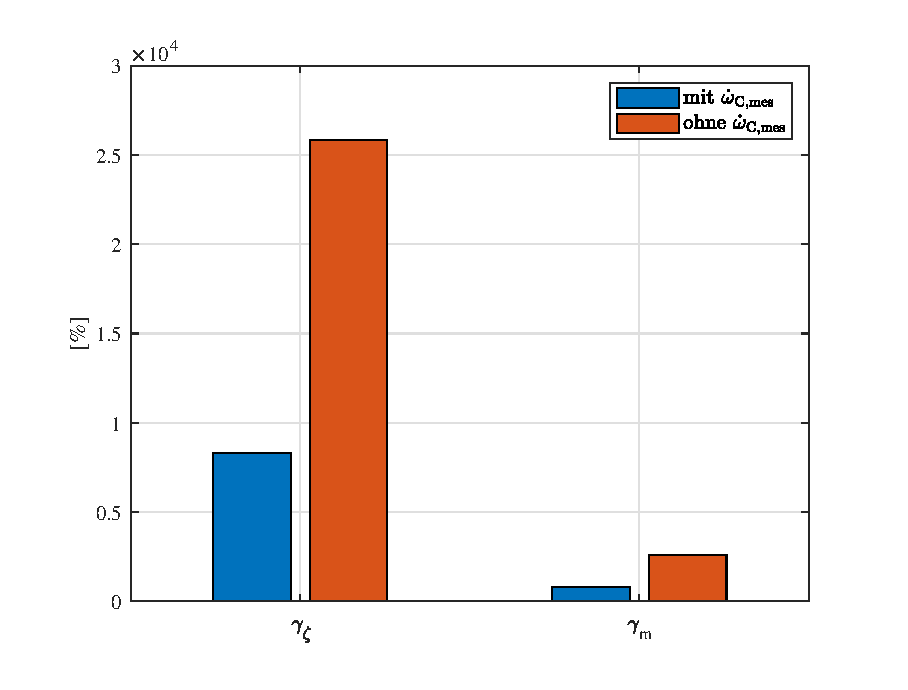
\includegraphics[scale=0.9]{figures/03_Sensitivitaetsanalyse/03_Fisher_Info/Gang2/m_vs_zeta.eps}
  \caption{Streuungen der Fisher-Informationsmatrix für die simultane Schätzung von $m$ und $\zeta$ im 2. Gang mit $\dot{\omega}_\mathrm{C,mes}$ als Messgröße und ohne.}
\end{figure} 

\begin{figure}[ht]
  \centering
 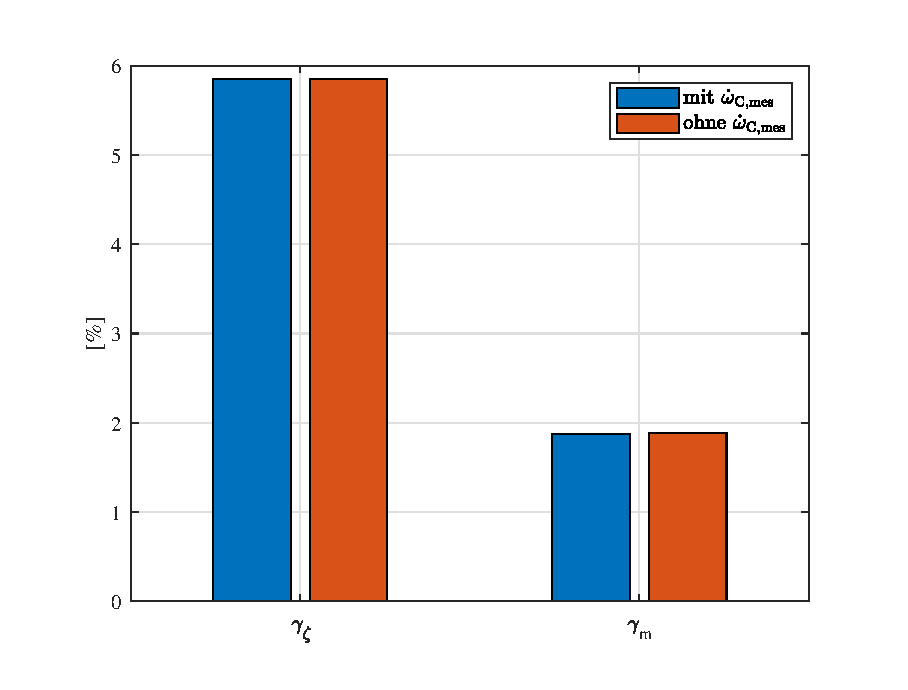
\includegraphics[scale=0.9]{figures/03_Sensitivitaetsanalyse/03_Fisher_Info/Gang2/m_vs_zeta_einzeln.eps}
  \caption{Streuungen der Fisher-Informationsmatrix für die einzelne Schätzung von $m$ und $\zeta$ im 2. Gang mit $\dot{\omega}_\mathrm{C,mes}$ als Messgröße und ohne.}
\end{figure} 

\subsection{Berechnung der Fisher-Informationsmatrix während der Momentenübergabe}

\begin{figure}[ht]
  \centering
 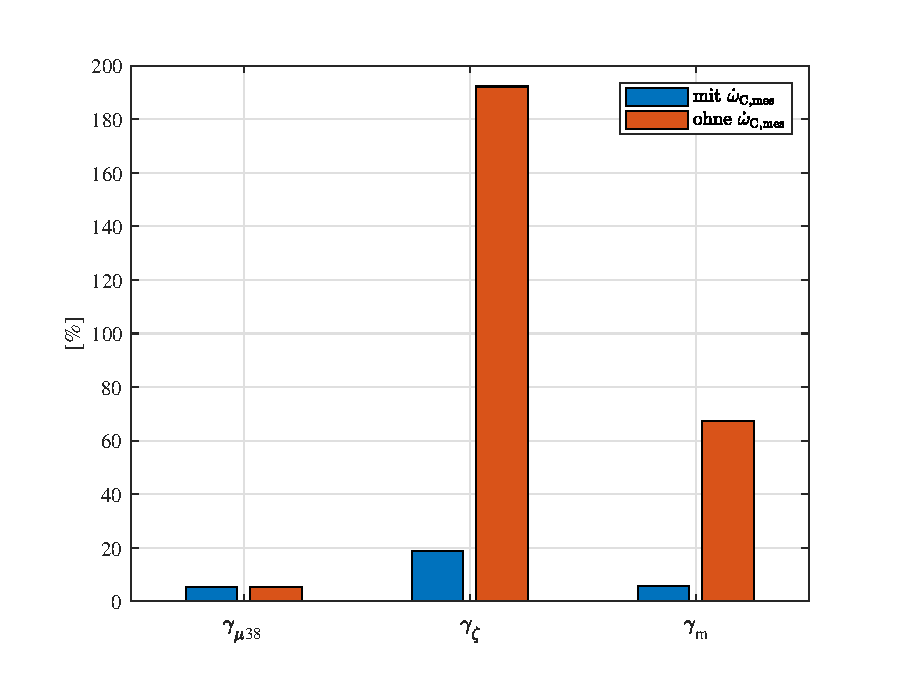
\includegraphics[scale=0.9]{figures/03_Sensitivitaetsanalyse/03_Fisher_Info/Muebergabe/m_mu38_zeta.eps}
  \caption{Streuungen der Fisher-Informationsmatrix für die simultane Schätzung von $m$, $\mu_{38}$ und $\zeta$ während der Momentenübergabe mit $\dot{\omega}_\mathrm{C,mes}$ als Messgröße und ohne.}
\end{figure} 

\begin{figure}[ht]
  \centering
 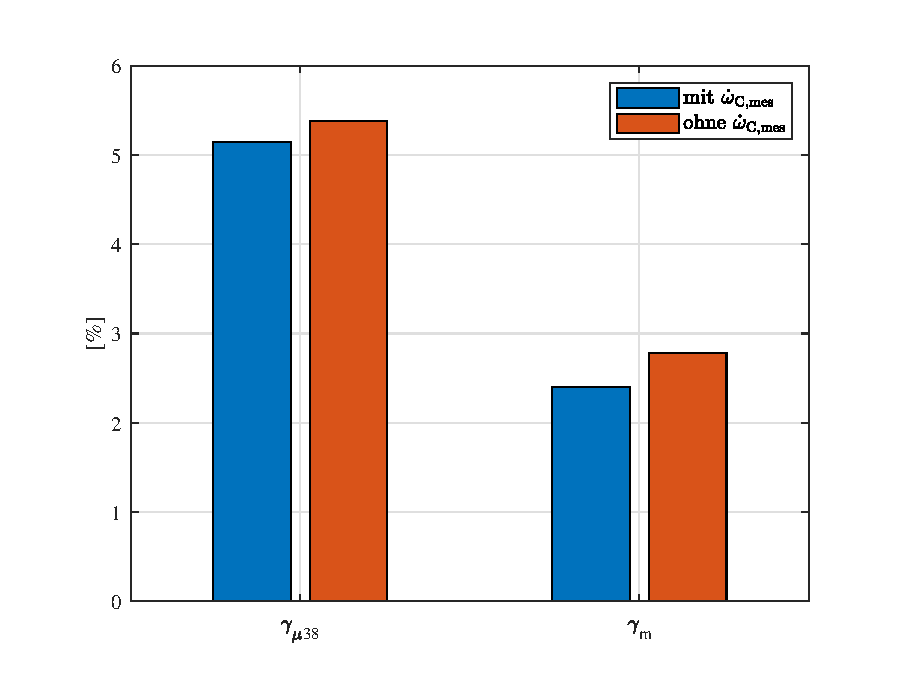
\includegraphics[scale=0.9]{figures/03_Sensitivitaetsanalyse/03_Fisher_Info/Muebergabe/m_mu38.eps}
  \caption{Streuungen der Fisher-Informationsmatrix für die simultane Schätzung von $m$, $\mu_{38}$ während der Momentenübergabe mit $\dot{\omega}_\mathrm{C,mes}$ als Messgröße und ohne.}
\end{figure} 

\begin{figure}[ht]
  \centering
 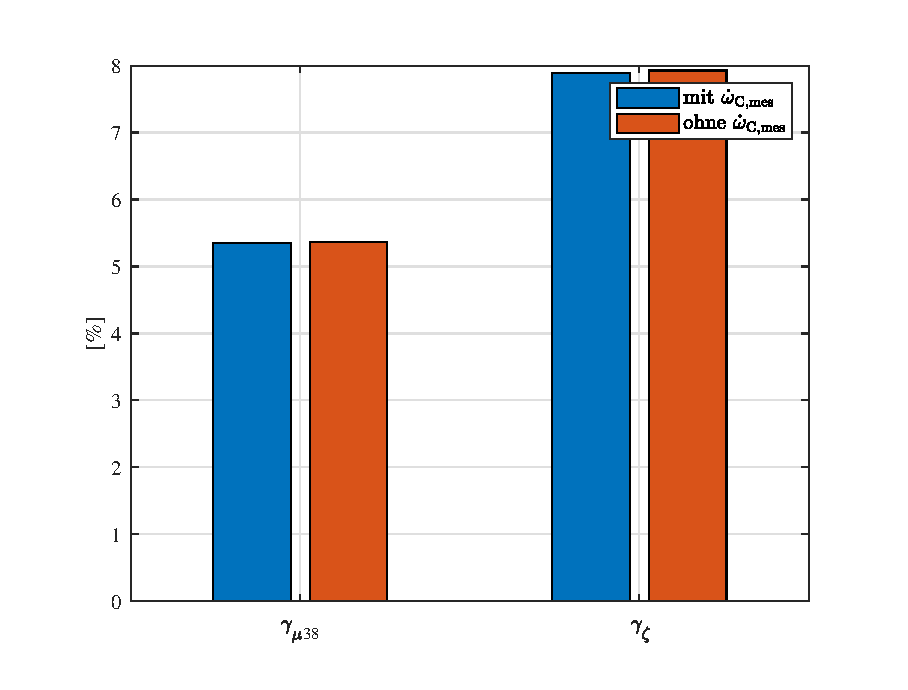
\includegraphics[scale=0.9]{figures/03_Sensitivitaetsanalyse/03_Fisher_Info/Muebergabe/mu38_zeta.eps}
  \caption{Streuungen der Fisher-Informationsmatrix für die simultane Schätzung von $\mu_{38}$ und $\zeta$ während der Momentenübergabe mit $\dot{\omega}_\mathrm{C,mes}$ als Messgröße und ohne.}
\end{figure} 

\subsection{Berechnung der Fisher-Informationsmatrix während der Synchronisation}

\begin{figure}[ht]
  \centering
 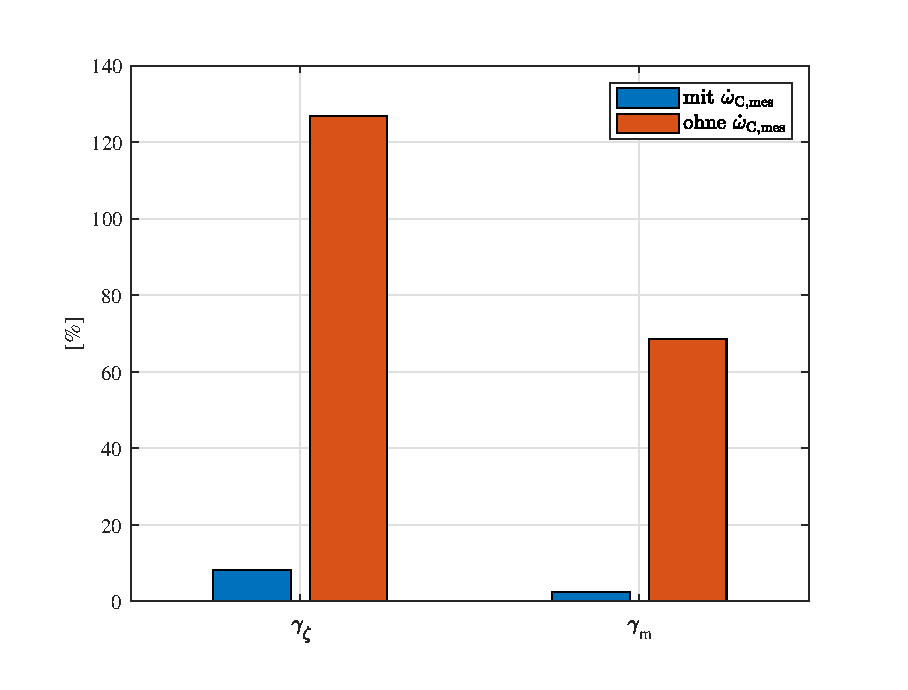
\includegraphics[scale=0.9]{figures/03_Sensitivitaetsanalyse/03_Fisher_Info/Sync/m_zeta_Sync.eps}
  \caption{Streuungen der Fisher-Informationsmatrix für die simultane Schätzung von $m$ und $\zeta$ während der Synchronisation mit $\dot{\omega}_\mathrm{C,mes}$ als Messgröße und ohne.}
\end{figure} 